\documentclass[twoside]{book}

% Packages required by doxygen
\usepackage{fixltx2e}
\usepackage{calc}
\usepackage{doxygen}
\usepackage[export]{adjustbox} % also loads graphicx
\usepackage{graphicx}
\usepackage[utf8]{inputenc}
\usepackage{makeidx}
\usepackage{multicol}
\usepackage{multirow}
\PassOptionsToPackage{warn}{textcomp}
\usepackage{textcomp}
\usepackage[nointegrals]{wasysym}
\usepackage[table]{xcolor}

% Font selection
\usepackage[T1]{fontenc}
\usepackage[scaled=.90]{helvet}
\usepackage{courier}
\usepackage{amssymb}
\usepackage{sectsty}
\renewcommand{\familydefault}{\sfdefault}
\allsectionsfont{%
  \fontseries{bc}\selectfont%
  \color{darkgray}%
}
\renewcommand{\DoxyLabelFont}{%
  \fontseries{bc}\selectfont%
  \color{darkgray}%
}
\newcommand{\+}{\discretionary{\mbox{\scriptsize$\hookleftarrow$}}{}{}}

% Page & text layout
\usepackage{geometry}
\geometry{%
  a4paper,%
  top=2.5cm,%
  bottom=2.5cm,%
  left=2.5cm,%
  right=2.5cm%
}
\tolerance=750
\hfuzz=15pt
\hbadness=750
\setlength{\emergencystretch}{15pt}
\setlength{\parindent}{0cm}
\setlength{\parskip}{3ex plus 2ex minus 2ex}
\makeatletter
\renewcommand{\paragraph}{%
  \@startsection{paragraph}{4}{0ex}{-1.0ex}{1.0ex}{%
    \normalfont\normalsize\bfseries\SS@parafont%
  }%
}
\renewcommand{\subparagraph}{%
  \@startsection{subparagraph}{5}{0ex}{-1.0ex}{1.0ex}{%
    \normalfont\normalsize\bfseries\SS@subparafont%
  }%
}
\makeatother

% Headers & footers
\usepackage{fancyhdr}
\pagestyle{fancyplain}
\fancyhead[LE]{\fancyplain{}{\bfseries\thepage}}
\fancyhead[CE]{\fancyplain{}{}}
\fancyhead[RE]{\fancyplain{}{\bfseries\leftmark}}
\fancyhead[LO]{\fancyplain{}{\bfseries\rightmark}}
\fancyhead[CO]{\fancyplain{}{}}
\fancyhead[RO]{\fancyplain{}{\bfseries\thepage}}
\fancyfoot[LE]{\fancyplain{}{}}
\fancyfoot[CE]{\fancyplain{}{}}
\fancyfoot[RE]{\fancyplain{}{\bfseries\scriptsize Generated by Doxygen }}
\fancyfoot[LO]{\fancyplain{}{\bfseries\scriptsize Generated by Doxygen }}
\fancyfoot[CO]{\fancyplain{}{}}
\fancyfoot[RO]{\fancyplain{}{}}
\renewcommand{\footrulewidth}{0.4pt}
\renewcommand{\chaptermark}[1]{%
  \markboth{#1}{}%
}
\renewcommand{\sectionmark}[1]{%
  \markright{\thesection\ #1}%
}

% Indices & bibliography
\usepackage{natbib}
\usepackage[titles]{tocloft}
\setcounter{tocdepth}{3}
\setcounter{secnumdepth}{5}
\makeindex

% Hyperlinks (required, but should be loaded last)
\usepackage{ifpdf}
\ifpdf
  \usepackage[pdftex,pagebackref=true]{hyperref}
\else
  \usepackage[ps2pdf,pagebackref=true]{hyperref}
\fi
\hypersetup{%
  colorlinks=true,%
  linkcolor=blue,%
  citecolor=blue,%
  unicode%
}

% Custom commands
\newcommand{\clearemptydoublepage}{%
  \newpage{\pagestyle{empty}\cleardoublepage}%
}

\usepackage{caption}
\captionsetup{labelsep=space,justification=centering,font={bf},singlelinecheck=off,skip=4pt,position=top}

%===== C O N T E N T S =====

\begin{document}

% Titlepage & ToC
\hypersetup{pageanchor=false,
             bookmarksnumbered=true,
             pdfencoding=unicode
            }
\pagenumbering{alph}
\begin{titlepage}
\vspace*{7cm}
\begin{center}%
{\Large C\+A\+D\+Tool }\\
\vspace*{1cm}
{\large Generated by Doxygen 1.8.14}\\
\end{center}
\end{titlepage}
\clearemptydoublepage
\pagenumbering{roman}
\tableofcontents
\clearemptydoublepage
\pagenumbering{arabic}
\hypersetup{pageanchor=true}

%--- Begin generated contents ---
\chapter{C\+AD Module}
\label{md__readme}
\Hypertarget{md__readme}
This application can be used to
\begin{DoxyEnumerate}
\item Generate Projections and Orthographic Views of 3D objects.
\end{DoxyEnumerate}


\begin{DoxyEnumerate}
\item Reconstruct 3D objects from orthographic projections.
\end{DoxyEnumerate}



\subsection*{Installing}

\begin{DoxyVerb}The app folder contains an AppImage which can run on Linux systems. 
Make the app executable by running 

chmod a+x CAD.AppImage 

in the app folder.
\end{DoxyVerb}


\#\#\# Build from sources \#\#\#\# 
\begin{DoxyCode}
qmake CAD.pro
make
\end{DoxyCode}


\subsection*{Format of Input}


\begin{DoxyEnumerate}
\item To Get 3D object provide a $\ast$.txt$\ast$ file containing the informaion about orthographic projections. \paragraph*{Format of $\ast$.txt$\ast$ file}
\end{DoxyEnumerate}

f 0 0 \# a vertex (0, 0) in front projection f 0 1 \# a vertex (0, 1) in front projection f ... ...

fe 1 2 \# an edge in front projection between vertices (0, 0) and (0, 1) fe ... ...

t 0 1 \# a vertex (0, 1) in top projection t 0 2 \# a vertex (0, 2) in top projection t 1 2 \# a vertex (1, 2) in top projection ...

te 1 3 \# an edge in side projection between vertices (0, 1) and (1, 2) te 2 3 \# an edge in side projection between vertices (0, 2) and (1, 2) ...

s 1 0 \# a vertex (1, 0) in side projection s 1 1 \# a vertex (1, 1) in side projection s ... ...

se 1 2 \# an edge in side projection between vertices (1, 0) and (1, 1) se ... ...

The application takes such a $\ast$.txt$\ast$ file and generates a $\ast$.obj$\ast$ file.


\begin{DoxyEnumerate}
\item To Generate Projections and Orthographic Views provide a $\ast$.obj$\ast$ file of the 3D object.
\end{DoxyEnumerate}

\paragraph*{Format of $\ast$.obj$\ast$ file}

v 1 2 3 \# a vertex \textquotesingle{}v\textquotesingle{} followed by (x, y, z) coordinates of the point v ... ...

f 1 3 4 \# a face \textquotesingle{}f\textquotesingle{} followed by indices of vertices lying on that plane f ... ...

The application takes such a $\ast$.obj$\ast$ file and generates a $\ast$.txt$\ast$ file.

\subsection*{Authors}


\begin{DoxyItemize}
\item {\bfseries \href{http://github.com/saranshiitd}{\tt Saransh Verma}}
\item {\bfseries \href{http://github.com/tarunyadav452}{\tt Tarun Kumar Yadav}} 
\end{DoxyItemize}
\chapter{Namespace Index}
\section{Namespace List}
Here is a list of all namespaces with brief descriptions\+:\begin{DoxyCompactList}
\item\contentsline{section}{\mbox{\hyperlink{namespacegeneral_methods}{general\+Methods}} }{\pageref{namespacegeneral_methods}}{}
\item\contentsline{section}{\mbox{\hyperlink{namespace_ui}{Ui}} }{\pageref{namespace_ui}}{}
\end{DoxyCompactList}

\chapter{Hierarchical Index}
\section{Class Hierarchy}
This inheritance list is sorted roughly, but not completely, alphabetically\+:\begin{DoxyCompactList}
\item \contentsline{section}{basic\+Loop\+Edge\+Set}{\pageref{classbasic_loop_edge_set}}{}
\item \contentsline{section}{body\+Loop}{\pageref{classbody_loop}}{}
\item \contentsline{section}{direction}{\pageref{structdirection}}{}
\item \contentsline{section}{edge2D}{\pageref{structedge2_d}}{}
\item \contentsline{section}{edge3D}{\pageref{structedge3_d}}{}
\item \contentsline{section}{Edge\+List2D}{\pageref{class_edge_list2_d}}{}
\item \contentsline{section}{edge\+Vertex\+Triplet}{\pageref{structedge_vertex_triplet}}{}
\item \contentsline{section}{face\+Loop}{\pageref{classface_loop}}{}
\item \contentsline{section}{plane}{\pageref{structplane}}{}
\item \contentsline{section}{Plane}{\pageref{class_plane}}{}
\item \contentsline{section}{plane\+V\+EL}{\pageref{structplane_v_e_l}}{}
\item Q\+Main\+Window\begin{DoxyCompactList}
\item \contentsline{section}{Main\+Window}{\pageref{class_main_window}}{}
\item \contentsline{section}{Selection}{\pageref{class_selection}}{}
\item \contentsline{section}{Show\+Projections}{\pageref{class_show_projections}}{}
\end{DoxyCompactList}
\item \contentsline{section}{qt\+\_\+meta\+\_\+stringdata\+\_\+\+Main\+Window\+\_\+t}{\pageref{structqt__meta__stringdata___main_window__t}}{}
\item \contentsline{section}{qt\+\_\+meta\+\_\+stringdata\+\_\+\+Options\+\_\+t}{\pageref{structqt__meta__stringdata___options__t}}{}
\item \contentsline{section}{qt\+\_\+meta\+\_\+stringdata\+\_\+\+Selection\+\_\+t}{\pageref{structqt__meta__stringdata___selection__t}}{}
\item \contentsline{section}{qt\+\_\+meta\+\_\+stringdata\+\_\+\+Show\+Projections\+\_\+t}{\pageref{structqt__meta__stringdata___show_projections__t}}{}
\item Q\+Widget\begin{DoxyCompactList}
\item \contentsline{section}{Options}{\pageref{class_options}}{}
\end{DoxyCompactList}
\item \contentsline{section}{Two\+D\+Obj}{\pageref{class_two_d_obj}}{}
\item \contentsline{section}{Ui\+\_\+\+Main\+Window}{\pageref{class_ui___main_window}}{}
\begin{DoxyCompactList}
\item \contentsline{section}{Ui\+:\+:Main\+Window}{\pageref{class_ui_1_1_main_window}}{}
\end{DoxyCompactList}
\item \contentsline{section}{Ui\+\_\+\+Selection}{\pageref{class_ui___selection}}{}
\begin{DoxyCompactList}
\item \contentsline{section}{Ui\+:\+:Selection}{\pageref{class_ui_1_1_selection}}{}
\end{DoxyCompactList}
\item \contentsline{section}{Ui\+\_\+\+Show\+Projections}{\pageref{class_ui___show_projections}}{}
\begin{DoxyCompactList}
\item \contentsline{section}{Ui\+:\+:Show\+Projections}{\pageref{class_ui_1_1_show_projections}}{}
\end{DoxyCompactList}
\item \contentsline{section}{vertex2D}{\pageref{structvertex2_d}}{}
\item \contentsline{section}{vertex3D}{\pageref{structvertex3_d}}{}
\item \contentsline{section}{vertex\+Edge\+List}{\pageref{structvertex_edge_list}}{}
\item \contentsline{section}{vertex\+Edge\+Pair}{\pageref{structvertex_edge_pair}}{}
\item \contentsline{section}{Vertex\+List2D}{\pageref{class_vertex_list2_d}}{}
\item \contentsline{section}{wire\+Frame}{\pageref{classwire_frame}}{}
\end{DoxyCompactList}

\chapter{Class Index}
\section{Class List}
Here are the classes, structs, unions and interfaces with brief descriptions\+:\begin{DoxyCompactList}
\item\contentsline{section}{\mbox{\hyperlink{structqt__meta__stringdata___main_window__t}{qt\+\_\+meta\+\_\+stringdata\+\_\+\+Main\+Window\+\_\+t}} }{\pageref{structqt__meta__stringdata___main_window__t}}{}
\item\contentsline{section}{\mbox{\hyperlink{structqt__meta__stringdata___options__t}{qt\+\_\+meta\+\_\+stringdata\+\_\+\+Options\+\_\+t}} }{\pageref{structqt__meta__stringdata___options__t}}{}
\item\contentsline{section}{\mbox{\hyperlink{structqt__meta__stringdata___selection__t}{qt\+\_\+meta\+\_\+stringdata\+\_\+\+Selection\+\_\+t}} }{\pageref{structqt__meta__stringdata___selection__t}}{}
\item\contentsline{section}{\mbox{\hyperlink{structqt__meta__stringdata___show_projections__t}{qt\+\_\+meta\+\_\+stringdata\+\_\+\+Show\+Projections\+\_\+t}} }{\pageref{structqt__meta__stringdata___show_projections__t}}{}
\end{DoxyCompactList}

\chapter{File Index}
\section{File List}
Here is a list of all files with brief descriptions\+:\begin{DoxyCompactList}
\item\contentsline{section}{build/\mbox{\hyperlink{build_2moc__mainwindow_8cpp}{moc\+\_\+mainwindow.\+cpp}} }{\pageref{build_2moc__mainwindow_8cpp}}{}
\item\contentsline{section}{build/\mbox{\hyperlink{build_2moc__options_8cpp}{moc\+\_\+options.\+cpp}} }{\pageref{build_2moc__options_8cpp}}{}
\item\contentsline{section}{build/\mbox{\hyperlink{build_2moc__selection_8cpp}{moc\+\_\+selection.\+cpp}} }{\pageref{build_2moc__selection_8cpp}}{}
\item\contentsline{section}{build/\mbox{\hyperlink{build_2moc__showprojections_8cpp}{moc\+\_\+showprojections.\+cpp}} }{\pageref{build_2moc__showprojections_8cpp}}{}
\item\contentsline{section}{include/\mbox{\hyperlink{basic_loop_edge_set_8h}{basic\+Loop\+Edge\+Set.\+h}} }{\pageref{basic_loop_edge_set_8h}}{}
\item\contentsline{section}{include/\mbox{\hyperlink{body_loop_8h}{body\+Loop.\+h}} }{\pageref{body_loop_8h}}{}
\item\contentsline{section}{include/\mbox{\hyperlink{_edge_list2_d_8h}{Edge\+List2\+D.\+h}} }{\pageref{_edge_list2_d_8h}}{}
\item\contentsline{section}{include/\mbox{\hyperlink{face_loop_8h}{face\+Loop.\+h}} }{\pageref{face_loop_8h}}{}
\item\contentsline{section}{include/\mbox{\hyperlink{general_methods_8h}{general\+Methods.\+h}} }{\pageref{general_methods_8h}}{}
\item\contentsline{section}{include/\mbox{\hyperlink{mainwindow_8h}{mainwindow.\+h}} }{\pageref{mainwindow_8h}}{}
\item\contentsline{section}{include/\mbox{\hyperlink{options_8h}{options.\+h}} }{\pageref{options_8h}}{}
\item\contentsline{section}{include/\mbox{\hyperlink{_plane_8h}{Plane.\+h}} }{\pageref{_plane_8h}}{}
\item\contentsline{section}{include/\mbox{\hyperlink{selection_8h}{selection.\+h}} }{\pageref{selection_8h}}{}
\item\contentsline{section}{include/\mbox{\hyperlink{showprojections_8h}{showprojections.\+h}} }{\pageref{showprojections_8h}}{}
\item\contentsline{section}{include/\mbox{\hyperlink{structs_8h}{structs.\+h}} }{\pageref{structs_8h}}{}
\item\contentsline{section}{include/\mbox{\hyperlink{_two_d_obj_8h}{Two\+D\+Obj.\+h}} }{\pageref{_two_d_obj_8h}}{}
\item\contentsline{section}{include/\mbox{\hyperlink{ui__mainwindow_8h}{ui\+\_\+mainwindow.\+h}} }{\pageref{ui__mainwindow_8h}}{}
\item\contentsline{section}{include/\mbox{\hyperlink{ui__selection_8h}{ui\+\_\+selection.\+h}} }{\pageref{ui__selection_8h}}{}
\item\contentsline{section}{include/\mbox{\hyperlink{ui__showprojections_8h}{ui\+\_\+showprojections.\+h}} }{\pageref{ui__showprojections_8h}}{}
\item\contentsline{section}{include/\mbox{\hyperlink{_vertex_list2_d_8h}{Vertex\+List2\+D.\+h}} }{\pageref{_vertex_list2_d_8h}}{}
\item\contentsline{section}{include/\mbox{\hyperlink{wireframe_8h}{wireframe.\+h}} }{\pageref{wireframe_8h}}{}
\item\contentsline{section}{src/\mbox{\hyperlink{basic_loop_edge_set_8cpp}{basic\+Loop\+Edge\+Set.\+cpp}} }{\pageref{basic_loop_edge_set_8cpp}}{}
\item\contentsline{section}{src/\mbox{\hyperlink{body_loop_8cpp}{body\+Loop.\+cpp}} }{\pageref{body_loop_8cpp}}{}
\item\contentsline{section}{src/\mbox{\hyperlink{_edge_list2_d_8cpp}{Edge\+List2\+D.\+cpp}} }{\pageref{_edge_list2_d_8cpp}}{}
\item\contentsline{section}{src/\mbox{\hyperlink{face_loop_8cpp}{face\+Loop.\+cpp}} }{\pageref{face_loop_8cpp}}{}
\item\contentsline{section}{src/\mbox{\hyperlink{general_methods_8cpp}{general\+Methods.\+cpp}} }{\pageref{general_methods_8cpp}}{}
\item\contentsline{section}{src/\mbox{\hyperlink{main_8cpp}{main.\+cpp}} }{\pageref{main_8cpp}}{}
\item\contentsline{section}{src/\mbox{\hyperlink{mainwindow_8cpp}{mainwindow.\+cpp}} }{\pageref{mainwindow_8cpp}}{}
\item\contentsline{section}{src/\mbox{\hyperlink{src_2moc__mainwindow_8cpp}{moc\+\_\+mainwindow.\+cpp}} }{\pageref{src_2moc__mainwindow_8cpp}}{}
\item\contentsline{section}{src/\mbox{\hyperlink{src_2moc__options_8cpp}{moc\+\_\+options.\+cpp}} }{\pageref{src_2moc__options_8cpp}}{}
\item\contentsline{section}{src/\mbox{\hyperlink{src_2moc__selection_8cpp}{moc\+\_\+selection.\+cpp}} }{\pageref{src_2moc__selection_8cpp}}{}
\item\contentsline{section}{src/\mbox{\hyperlink{src_2moc__showprojections_8cpp}{moc\+\_\+showprojections.\+cpp}} }{\pageref{src_2moc__showprojections_8cpp}}{}
\item\contentsline{section}{src/\mbox{\hyperlink{options_8cpp}{options.\+cpp}} }{\pageref{options_8cpp}}{}
\item\contentsline{section}{src/\mbox{\hyperlink{_plane_8cpp}{Plane.\+cpp}} }{\pageref{_plane_8cpp}}{}
\item\contentsline{section}{src/\mbox{\hyperlink{selection_8cpp}{selection.\+cpp}} }{\pageref{selection_8cpp}}{}
\item\contentsline{section}{src/\mbox{\hyperlink{showprojections_8cpp}{showprojections.\+cpp}} }{\pageref{showprojections_8cpp}}{}
\item\contentsline{section}{src/\mbox{\hyperlink{structs_8cpp}{structs.\+cpp}} }{\pageref{structs_8cpp}}{}
\item\contentsline{section}{src/\mbox{\hyperlink{_two_d_obj_8cpp}{Two\+D\+Obj.\+cpp}} }{\pageref{_two_d_obj_8cpp}}{}
\item\contentsline{section}{src/\mbox{\hyperlink{_vertex_list2_d_8cpp}{Vertex\+List2\+D.\+cpp}} }{\pageref{_vertex_list2_d_8cpp}}{}
\item\contentsline{section}{src/\mbox{\hyperlink{wireframe_8cpp}{wireframe.\+cpp}} }{\pageref{wireframe_8cpp}}{}
\end{DoxyCompactList}

\chapter{Namespace Documentation}
\hypertarget{namespacegeneral_methods}{}\section{general\+Methods Namespace Reference}
\label{namespacegeneral_methods}\index{general\+Methods@{general\+Methods}}
\subsection*{Functions}
\begin{DoxyCompactItemize}
\item 
void \mbox{\hyperlink{namespacegeneral_methods_a694306c7472ee1bbfb3c90c0f3d5453a}{print\+Vertex}} (\mbox{\hyperlink{structvertex3_d}{vertex3D}} i)
\begin{DoxyCompactList}\small\item\em print methods \end{DoxyCompactList}\item 
void \mbox{\hyperlink{namespacegeneral_methods_a9cbf7d7c2019f0e2b6f9773b687b50cd}{print\+Vertices\+List}} (vector$<$ \mbox{\hyperlink{structvertex3_d}{vertex3D}} $>$ v)
\item 
void \mbox{\hyperlink{namespacegeneral_methods_af9a1c28dacf89e746b51916fe178ce1a}{print\+Edge}} (\mbox{\hyperlink{structedge3_d}{edge3D}} i)
\item 
void \mbox{\hyperlink{namespacegeneral_methods_ab6b6f8a5d92b39ead6c97ec0917b75a4}{print\+Edge\+List}} (vector$<$ \mbox{\hyperlink{structedge3_d}{edge3D}} $>$ e)
\item 
void \mbox{\hyperlink{namespacegeneral_methods_a3474d24f9f545407bb5f73250a5e19d7}{print\+Plane}} (\mbox{\hyperlink{structplane}{plane}} p)
\item 
void \mbox{\hyperlink{namespacegeneral_methods_aa7c9b8abc94ae6b08d2cf083a08eaf21}{print\+Planes}} (vector$<$ \mbox{\hyperlink{structplane}{plane}} $>$ p)
\item 
void \mbox{\hyperlink{namespacegeneral_methods_a60a9e0ba058824389fc703dc2dbbb7e3}{print\+V\+E\+List}} (\mbox{\hyperlink{structvertex_edge_list}{vertex\+Edge\+List}} ve\+List)
\item 
void \mbox{\hyperlink{namespacegeneral_methods_adc8e104a2f2ed35a22be9a68051ec38d}{printplane\+V\+EL}} (\mbox{\hyperlink{structplane_v_e_l}{plane\+V\+EL}} p)
\item 
std\+::vector$<$ \mbox{\hyperlink{structvertex3_d}{vertex3D}} $>$ \mbox{\hyperlink{namespacegeneral_methods_ace3487740f3b46dce9e0357366abf9ed}{sort\+Vertices}} (std\+::vector$<$ \mbox{\hyperlink{structvertex3_d}{vertex3D}} $>$ V, \mbox{\hyperlink{structedge3_d}{edge3D}} e)
\item 
bool \mbox{\hyperlink{namespacegeneral_methods_aa7662b2bcff30f8983da23da5edfc766}{check\+Overlap\+Collinear}} (\mbox{\hyperlink{structedge3_d}{edge3D}} e1, \mbox{\hyperlink{structedge3_d}{edge3D}} e2)
\item 
bool \mbox{\hyperlink{namespacegeneral_methods_a508d15a0c76920dc4f98cf8da254f9c4}{check\+Coplanar}} (\mbox{\hyperlink{structedge3_d}{edge3D}} e1, \mbox{\hyperlink{structedge3_d}{edge3D}} e2, \mbox{\hyperlink{structedge3_d}{edge3D}} e3)
\item 
\mbox{\hyperlink{structplane}{plane}} \mbox{\hyperlink{namespacegeneral_methods_a06d99f1b292d29dbdbe4734847c8d2ee}{make\+Plane}} (\mbox{\hyperlink{structedge3_d}{edge3D}} e1, \mbox{\hyperlink{structedge3_d}{edge3D}} e2)
\item 
std\+::vector$<$ \mbox{\hyperlink{structplane}{plane}} $>$ \mbox{\hyperlink{namespacegeneral_methods_a13072e8b14fcea9ae253085569062158}{remove\+Duplicate}} (std\+::vector$<$ \mbox{\hyperlink{structplane}{plane}} $>$ v)
\item 
float \mbox{\hyperlink{namespacegeneral_methods_a3bc88a001e751ad419e87bf3795ca02b}{find\+Distance\+Between\+Planes}} (\mbox{\hyperlink{structplane}{plane}} p, \mbox{\hyperlink{structplane}{plane}} q)
\item 
bool \mbox{\hyperlink{namespacegeneral_methods_a21d2e8c181e8cac3762d9ca1871d2168}{if\+Edge\+On\+Plane}} (\mbox{\hyperlink{structplane}{plane}} p, \mbox{\hyperlink{structedge3_d}{edge3D}} e)
\item 
bool \mbox{\hyperlink{namespacegeneral_methods_a330682bb45234d8de5228a7607d493d2}{if\+Vertex\+On\+Plane}} (\mbox{\hyperlink{structplane}{plane}} p, \mbox{\hyperlink{structvertex3_d}{vertex3D}} v)
\item 
std\+::vector$<$ \mbox{\hyperlink{structedge3_d}{edge3D}} $>$ \mbox{\hyperlink{namespacegeneral_methods_a9bff72be73e4d6faec798a23b8f28cb9}{find\+Edges\+On\+Plane}} (\mbox{\hyperlink{structplane}{plane}} p, std\+::vector$<$ \mbox{\hyperlink{structedge3_d}{edge3D}} $>$ e\+List)
\item 
std\+::vector$<$ \mbox{\hyperlink{structvertex3_d}{vertex3D}} $>$ \mbox{\hyperlink{namespacegeneral_methods_aa0669678cf59876e3249ddce7a0d1ce3}{find\+Vertices\+On\+Plane}} (\mbox{\hyperlink{structplane}{plane}} p, std\+::vector$<$ \mbox{\hyperlink{structvertex3_d}{vertex3D}} $>$ eop)
\item 
bool \mbox{\hyperlink{namespacegeneral_methods_a44d97941601f5929b217570ba9027d27}{check\+Hidden}} (\mbox{\hyperlink{structplane}{plane}} p, \mbox{\hyperlink{structedge3_d}{edge3D}} e, float \mbox{\hyperlink{structdirection}{direction}})
\item 
int \mbox{\hyperlink{namespacegeneral_methods_a2bb810600ec90ec064ea8496ee0ab862}{check\+Confinement}} (\mbox{\hyperlink{classbasic_loop_edge_set}{basic\+Loop\+Edge\+Set}} fl1, \mbox{\hyperlink{classbasic_loop_edge_set}{basic\+Loop\+Edge\+Set}} fl2, \mbox{\hyperlink{structplane}{plane}} p)
\item 
float $\ast$ \mbox{\hyperlink{namespacegeneral_methods_a0bd9c59442b6f9c7fd3ae00832ee30df}{get\+Alpha\+And\+Direction}} (\mbox{\hyperlink{classface_loop}{face\+Loop}} flk, \mbox{\hyperlink{classface_loop}{face\+Loop}} fls, \mbox{\hyperlink{structedge3_d}{edge3D}} reference\+Edge)
\item 
bool \mbox{\hyperlink{namespacegeneral_methods_a4ebb8d563530558e025b62c647045efe}{get\+If\+Outer}} (\mbox{\hyperlink{classbody_loop}{body\+Loop}} b)
\item 
bool \mbox{\hyperlink{namespacegeneral_methods_a557bf2257d6658862b42124035aa9588}{on\+Segment}} (\mbox{\hyperlink{structvertex3_d}{vertex3D}} v, \mbox{\hyperlink{structedge3_d}{edge3D}} edge)
\item 
int \mbox{\hyperlink{namespacegeneral_methods_a7bfbfb2a02328d76e70f66fedd57c4ef}{orientation}} (\mbox{\hyperlink{structvertex3_d}{vertex3D}} p, \mbox{\hyperlink{structvertex3_d}{vertex3D}} q, \mbox{\hyperlink{structvertex3_d}{vertex3D}} r, \mbox{\hyperlink{structplane}{plane}} s)
\item 
bool \mbox{\hyperlink{namespacegeneral_methods_a56efd049c58aae30a7b0caf39beab615}{do\+Intersect}} (\mbox{\hyperlink{structvertex3_d}{vertex3D}} p1, \mbox{\hyperlink{structvertex3_d}{vertex3D}} q1, \mbox{\hyperlink{structvertex3_d}{vertex3D}} p2, \mbox{\hyperlink{structvertex3_d}{vertex3D}} q2, \mbox{\hyperlink{structplane}{plane}} p)
\item 
bool \mbox{\hyperlink{namespacegeneral_methods_a27b7ed292415027c495942147e8856b7}{is\+Inside}} (std\+::vector$<$ \mbox{\hyperlink{structvertex3_d}{vertex3D}} $>$ polygon, int n, \mbox{\hyperlink{structvertex3_d}{vertex3D}} p, \mbox{\hyperlink{structedge3_d}{edge3D}} ref\+Edge, \mbox{\hyperlink{structplane}{plane}} q)
\item 
\mbox{\hyperlink{classface_loop}{face\+Loop}} \mbox{\hyperlink{namespacegeneral_methods_afe4087e253b318326a0a1578d34b42ca}{get\+Reversed\+Face\+Loop}} (\mbox{\hyperlink{classface_loop}{face\+Loop}} faceloop)
\item 
bool \mbox{\hyperlink{namespacegeneral_methods_afc8f20af710f8dc24af591015acc1403}{compare\+Pairs}} (\mbox{\hyperlink{structvertex_edge_pair}{vertex\+Edge\+Pair}} pair1, \mbox{\hyperlink{structvertex_edge_pair}{vertex\+Edge\+Pair}} pair2)
\item 
bool \mbox{\hyperlink{namespacegeneral_methods_a3c49599a5ba8f2c41f2ef542bde19765}{plane\+Equal}} (\mbox{\hyperlink{structplane}{plane}} p1, \mbox{\hyperlink{structplane}{plane}} p2)
\item 
bool \mbox{\hyperlink{namespacegeneral_methods_ab4e1b4b0a8b5b7697adddbb27950e639}{check\+Hidden}} (\mbox{\hyperlink{structplane}{plane}} p, \mbox{\hyperlink{structedge3_d}{edge3D}} e, float \mbox{\hyperlink{structdirection}{direction}}\mbox{[}$\,$\mbox{]})
\end{DoxyCompactItemize}


\subsection{Function Documentation}
\mbox{\Hypertarget{namespacegeneral_methods_a2bb810600ec90ec064ea8496ee0ab862}\label{namespacegeneral_methods_a2bb810600ec90ec064ea8496ee0ab862}} 
\index{general\+Methods@{general\+Methods}!check\+Confinement@{check\+Confinement}}
\index{check\+Confinement@{check\+Confinement}!general\+Methods@{general\+Methods}}
\subsubsection{\texorpdfstring{check\+Confinement()}{checkConfinement()}}
{\footnotesize\ttfamily int general\+Methods\+::check\+Confinement (\begin{DoxyParamCaption}\item[{\mbox{\hyperlink{classbasic_loop_edge_set}{basic\+Loop\+Edge\+Set}}}]{fl1,  }\item[{\mbox{\hyperlink{classbasic_loop_edge_set}{basic\+Loop\+Edge\+Set}}}]{fl2,  }\item[{\mbox{\hyperlink{structplane}{plane}}}]{p }\end{DoxyParamCaption})}

H\+OW TO C\+H\+E\+CK H\+I\+D\+D\+EN \+: first check both end points of edge lie on same side of plane substitute the take product and multiply result should be greater than 0 take an obnoxiously large coordinate in the direction you want to see like if you are observing from +y direction put (0,I\+NF,0) where I\+NF is large number take a point and return if substitution product less than 0 

Definition at line 369 of file general\+Methods.\+cpp.

Here is the call graph for this function\+:
\nopagebreak
\begin{figure}[H]
\begin{center}
\leavevmode
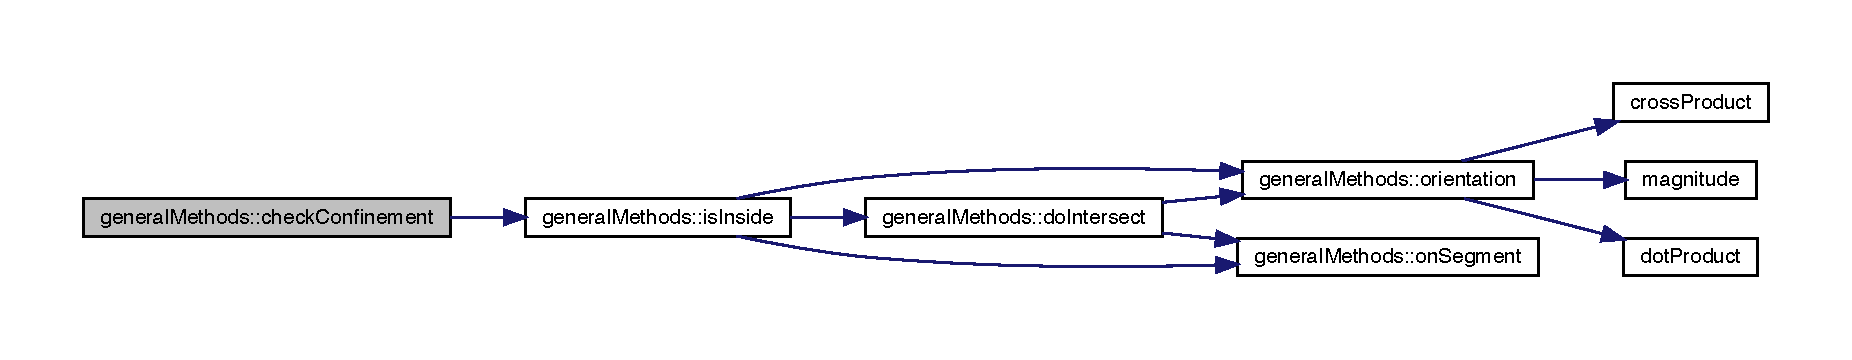
\includegraphics[width=350pt]{namespacegeneral_methods_a2bb810600ec90ec064ea8496ee0ab862_cgraph}
\end{center}
\end{figure}
Here is the caller graph for this function\+:
\nopagebreak
\begin{figure}[H]
\begin{center}
\leavevmode
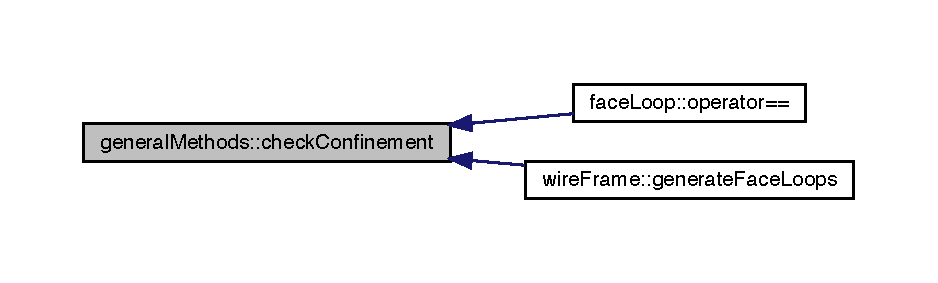
\includegraphics[width=350pt]{namespacegeneral_methods_a2bb810600ec90ec064ea8496ee0ab862_icgraph}
\end{center}
\end{figure}
\mbox{\Hypertarget{namespacegeneral_methods_a508d15a0c76920dc4f98cf8da254f9c4}\label{namespacegeneral_methods_a508d15a0c76920dc4f98cf8da254f9c4}} 
\index{general\+Methods@{general\+Methods}!check\+Coplanar@{check\+Coplanar}}
\index{check\+Coplanar@{check\+Coplanar}!general\+Methods@{general\+Methods}}
\subsubsection{\texorpdfstring{check\+Coplanar()}{checkCoplanar()}}
{\footnotesize\ttfamily bool general\+Methods\+::check\+Coplanar (\begin{DoxyParamCaption}\item[{\mbox{\hyperlink{structedge3_d}{edge3D}}}]{e1,  }\item[{\mbox{\hyperlink{structedge3_d}{edge3D}}}]{e2,  }\item[{\mbox{\hyperlink{structedge3_d}{edge3D}}}]{e3 }\end{DoxyParamCaption})}

check whether two edges coplanar 

Definition at line 163 of file general\+Methods.\+cpp.

Here is the call graph for this function\+:
\nopagebreak
\begin{figure}[H]
\begin{center}
\leavevmode
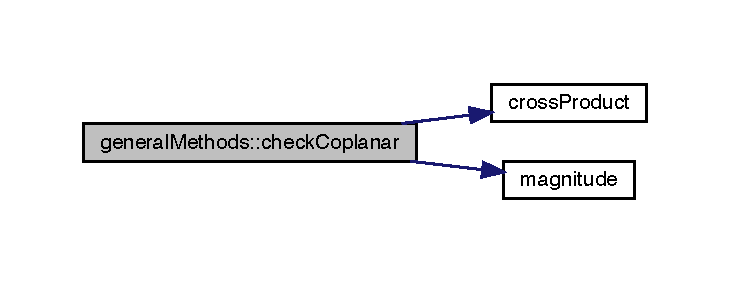
\includegraphics[width=350pt]{namespacegeneral_methods_a508d15a0c76920dc4f98cf8da254f9c4_cgraph}
\end{center}
\end{figure}
Here is the caller graph for this function\+:
\nopagebreak
\begin{figure}[H]
\begin{center}
\leavevmode
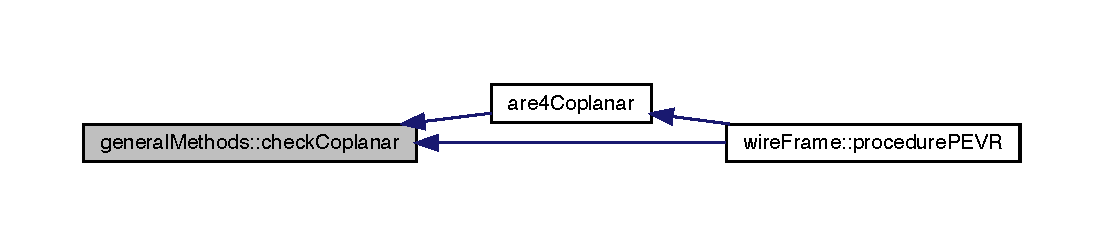
\includegraphics[width=350pt]{namespacegeneral_methods_a508d15a0c76920dc4f98cf8da254f9c4_icgraph}
\end{center}
\end{figure}
\mbox{\Hypertarget{namespacegeneral_methods_a44d97941601f5929b217570ba9027d27}\label{namespacegeneral_methods_a44d97941601f5929b217570ba9027d27}} 
\index{general\+Methods@{general\+Methods}!check\+Hidden@{check\+Hidden}}
\index{check\+Hidden@{check\+Hidden}!general\+Methods@{general\+Methods}}
\subsubsection{\texorpdfstring{check\+Hidden()}{checkHidden()}\hspace{0.1cm}{\footnotesize\ttfamily [1/2]}}
{\footnotesize\ttfamily bool general\+Methods\+::check\+Hidden (\begin{DoxyParamCaption}\item[{\mbox{\hyperlink{structplane}{plane}}}]{p,  }\item[{\mbox{\hyperlink{structedge3_d}{edge3D}}}]{e,  }\item[{float}]{direction }\end{DoxyParamCaption})}

check if plane hides an edge from direction \mbox{\Hypertarget{namespacegeneral_methods_ab4e1b4b0a8b5b7697adddbb27950e639}\label{namespacegeneral_methods_ab4e1b4b0a8b5b7697adddbb27950e639}} 
\index{general\+Methods@{general\+Methods}!check\+Hidden@{check\+Hidden}}
\index{check\+Hidden@{check\+Hidden}!general\+Methods@{general\+Methods}}
\subsubsection{\texorpdfstring{check\+Hidden()}{checkHidden()}\hspace{0.1cm}{\footnotesize\ttfamily [2/2]}}
{\footnotesize\ttfamily bool general\+Methods\+::check\+Hidden (\begin{DoxyParamCaption}\item[{\mbox{\hyperlink{structplane}{plane}}}]{p,  }\item[{\mbox{\hyperlink{structedge3_d}{edge3D}}}]{e,  }\item[{float}]{direction\mbox{[}$\,$\mbox{]} }\end{DoxyParamCaption})}



Definition at line 251 of file general\+Methods.\+cpp.

\mbox{\Hypertarget{namespacegeneral_methods_aa7662b2bcff30f8983da23da5edfc766}\label{namespacegeneral_methods_aa7662b2bcff30f8983da23da5edfc766}} 
\index{general\+Methods@{general\+Methods}!check\+Overlap\+Collinear@{check\+Overlap\+Collinear}}
\index{check\+Overlap\+Collinear@{check\+Overlap\+Collinear}!general\+Methods@{general\+Methods}}
\subsubsection{\texorpdfstring{check\+Overlap\+Collinear()}{checkOverlapCollinear()}}
{\footnotesize\ttfamily bool general\+Methods\+::check\+Overlap\+Collinear (\begin{DoxyParamCaption}\item[{\mbox{\hyperlink{structedge3_d}{edge3D}}}]{e1,  }\item[{\mbox{\hyperlink{structedge3_d}{edge3D}}}]{e2 }\end{DoxyParamCaption})}

-\/-\/-\/-\/-\/-\/-\/-\/-\/-\/-\/------methods of edges-\/-\/-\/-\/-\/-\/-\/-\/-\/-\/-\/-\/-\/-\/-\/-\/-\/-\/-\/-\/-\/-\/-\/------ ~\newline
check if edges overlap and collinear 

Definition at line 126 of file general\+Methods.\+cpp.

Here is the call graph for this function\+:
\nopagebreak
\begin{figure}[H]
\begin{center}
\leavevmode
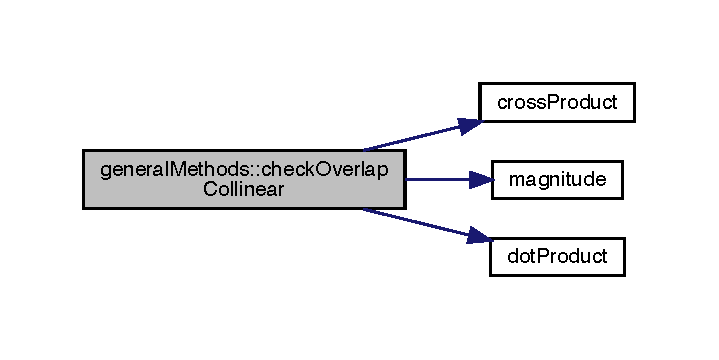
\includegraphics[width=345pt]{namespacegeneral_methods_aa7662b2bcff30f8983da23da5edfc766_cgraph}
\end{center}
\end{figure}
Here is the caller graph for this function\+:
\nopagebreak
\begin{figure}[H]
\begin{center}
\leavevmode
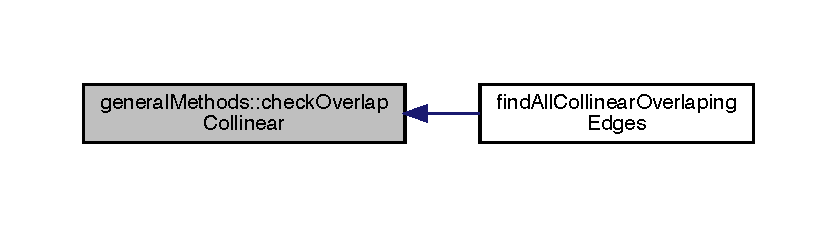
\includegraphics[width=350pt]{namespacegeneral_methods_aa7662b2bcff30f8983da23da5edfc766_icgraph}
\end{center}
\end{figure}
\mbox{\Hypertarget{namespacegeneral_methods_afc8f20af710f8dc24af591015acc1403}\label{namespacegeneral_methods_afc8f20af710f8dc24af591015acc1403}} 
\index{general\+Methods@{general\+Methods}!compare\+Pairs@{compare\+Pairs}}
\index{compare\+Pairs@{compare\+Pairs}!general\+Methods@{general\+Methods}}
\subsubsection{\texorpdfstring{compare\+Pairs()}{comparePairs()}}
{\footnotesize\ttfamily bool general\+Methods\+::compare\+Pairs (\begin{DoxyParamCaption}\item[{\mbox{\hyperlink{structvertex_edge_pair}{vertex\+Edge\+Pair}}}]{pair1,  }\item[{\mbox{\hyperlink{structvertex_edge_pair}{vertex\+Edge\+Pair}}}]{pair2 }\end{DoxyParamCaption})}



Definition at line 95 of file general\+Methods.\+cpp.

Here is the call graph for this function\+:
\nopagebreak
\begin{figure}[H]
\begin{center}
\leavevmode
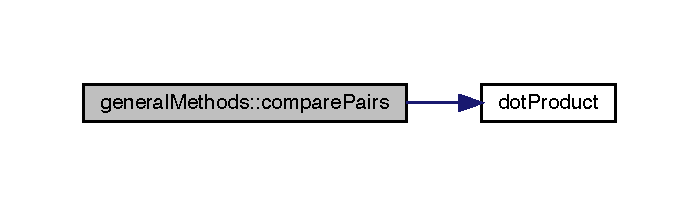
\includegraphics[width=335pt]{namespacegeneral_methods_afc8f20af710f8dc24af591015acc1403_cgraph}
\end{center}
\end{figure}
Here is the caller graph for this function\+:
\nopagebreak
\begin{figure}[H]
\begin{center}
\leavevmode
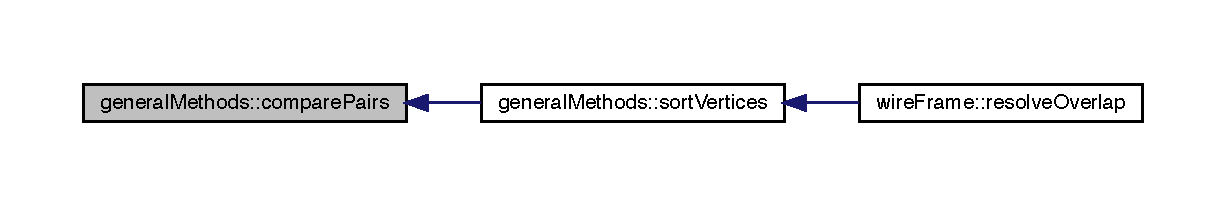
\includegraphics[width=350pt]{namespacegeneral_methods_afc8f20af710f8dc24af591015acc1403_icgraph}
\end{center}
\end{figure}
\mbox{\Hypertarget{namespacegeneral_methods_a56efd049c58aae30a7b0caf39beab615}\label{namespacegeneral_methods_a56efd049c58aae30a7b0caf39beab615}} 
\index{general\+Methods@{general\+Methods}!do\+Intersect@{do\+Intersect}}
\index{do\+Intersect@{do\+Intersect}!general\+Methods@{general\+Methods}}
\subsubsection{\texorpdfstring{do\+Intersect()}{doIntersect()}}
{\footnotesize\ttfamily bool general\+Methods\+::do\+Intersect (\begin{DoxyParamCaption}\item[{\mbox{\hyperlink{structvertex3_d}{vertex3D}}}]{p1,  }\item[{\mbox{\hyperlink{structvertex3_d}{vertex3D}}}]{q1,  }\item[{\mbox{\hyperlink{structvertex3_d}{vertex3D}}}]{p2,  }\item[{\mbox{\hyperlink{structvertex3_d}{vertex3D}}}]{q2,  }\item[{\mbox{\hyperlink{structplane}{plane}}}]{p }\end{DoxyParamCaption})}



Definition at line 295 of file general\+Methods.\+cpp.

Here is the call graph for this function\+:
\nopagebreak
\begin{figure}[H]
\begin{center}
\leavevmode
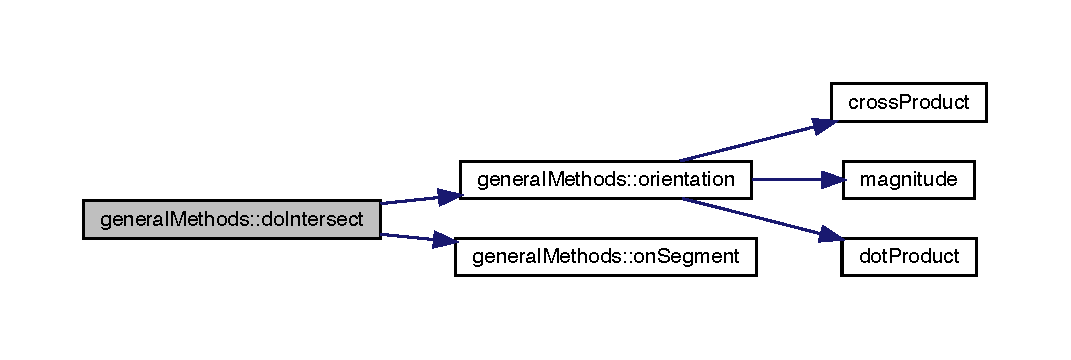
\includegraphics[width=350pt]{namespacegeneral_methods_a56efd049c58aae30a7b0caf39beab615_cgraph}
\end{center}
\end{figure}
Here is the caller graph for this function\+:
\nopagebreak
\begin{figure}[H]
\begin{center}
\leavevmode
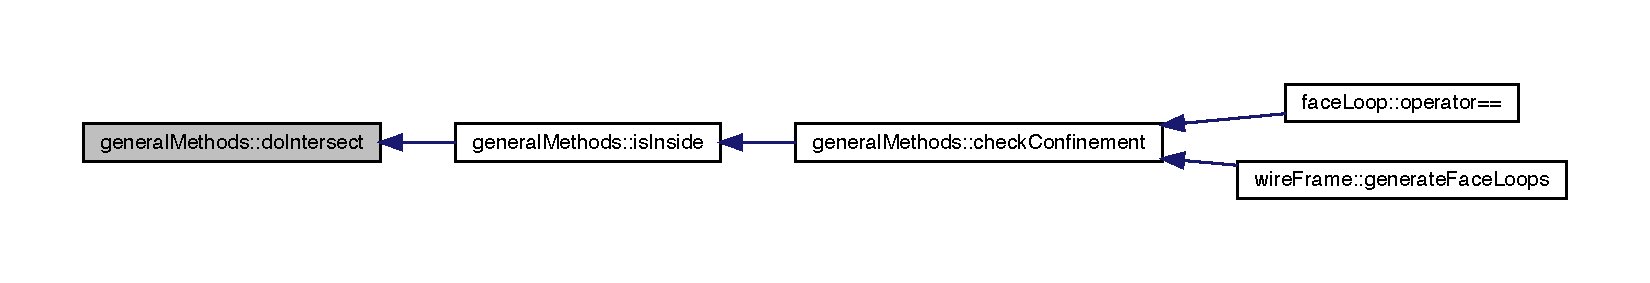
\includegraphics[width=350pt]{namespacegeneral_methods_a56efd049c58aae30a7b0caf39beab615_icgraph}
\end{center}
\end{figure}
\mbox{\Hypertarget{namespacegeneral_methods_a3bc88a001e751ad419e87bf3795ca02b}\label{namespacegeneral_methods_a3bc88a001e751ad419e87bf3795ca02b}} 
\index{general\+Methods@{general\+Methods}!find\+Distance\+Between\+Planes@{find\+Distance\+Between\+Planes}}
\index{find\+Distance\+Between\+Planes@{find\+Distance\+Between\+Planes}!general\+Methods@{general\+Methods}}
\subsubsection{\texorpdfstring{find\+Distance\+Between\+Planes()}{findDistanceBetweenPlanes()}}
{\footnotesize\ttfamily float general\+Methods\+::find\+Distance\+Between\+Planes (\begin{DoxyParamCaption}\item[{\mbox{\hyperlink{structplane}{plane}}}]{p,  }\item[{\mbox{\hyperlink{structplane}{plane}}}]{q }\end{DoxyParamCaption})}

returns distance between two planes 

Definition at line 206 of file general\+Methods.\+cpp.

\mbox{\Hypertarget{namespacegeneral_methods_a9bff72be73e4d6faec798a23b8f28cb9}\label{namespacegeneral_methods_a9bff72be73e4d6faec798a23b8f28cb9}} 
\index{general\+Methods@{general\+Methods}!find\+Edges\+On\+Plane@{find\+Edges\+On\+Plane}}
\index{find\+Edges\+On\+Plane@{find\+Edges\+On\+Plane}!general\+Methods@{general\+Methods}}
\subsubsection{\texorpdfstring{find\+Edges\+On\+Plane()}{findEdgesOnPlane()}}
{\footnotesize\ttfamily std\+::vector$<$ \mbox{\hyperlink{structedge3_d}{edge3D}} $>$ general\+Methods\+::find\+Edges\+On\+Plane (\begin{DoxyParamCaption}\item[{\mbox{\hyperlink{structplane}{plane}}}]{p,  }\item[{std\+::vector$<$ \mbox{\hyperlink{structedge3_d}{edge3D}} $>$}]{e\+List }\end{DoxyParamCaption})}

takes a plane and e\+\_\+list and returns the list of edges on that plane 

Definition at line 227 of file general\+Methods.\+cpp.

Here is the call graph for this function\+:
\nopagebreak
\begin{figure}[H]
\begin{center}
\leavevmode
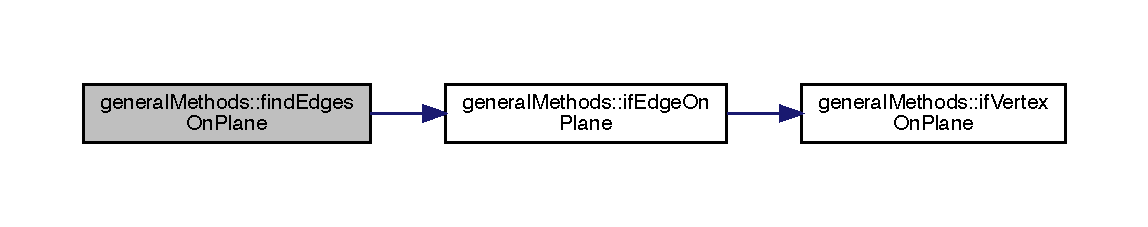
\includegraphics[width=350pt]{namespacegeneral_methods_a9bff72be73e4d6faec798a23b8f28cb9_cgraph}
\end{center}
\end{figure}
Here is the caller graph for this function\+:
\nopagebreak
\begin{figure}[H]
\begin{center}
\leavevmode
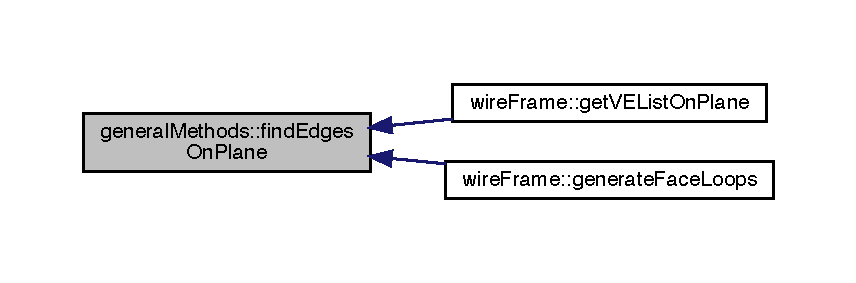
\includegraphics[width=350pt]{namespacegeneral_methods_a9bff72be73e4d6faec798a23b8f28cb9_icgraph}
\end{center}
\end{figure}
\mbox{\Hypertarget{namespacegeneral_methods_aa0669678cf59876e3249ddce7a0d1ce3}\label{namespacegeneral_methods_aa0669678cf59876e3249ddce7a0d1ce3}} 
\index{general\+Methods@{general\+Methods}!find\+Vertices\+On\+Plane@{find\+Vertices\+On\+Plane}}
\index{find\+Vertices\+On\+Plane@{find\+Vertices\+On\+Plane}!general\+Methods@{general\+Methods}}
\subsubsection{\texorpdfstring{find\+Vertices\+On\+Plane()}{findVerticesOnPlane()}}
{\footnotesize\ttfamily std\+::vector$<$ \mbox{\hyperlink{structvertex3_d}{vertex3D}} $>$ general\+Methods\+::find\+Vertices\+On\+Plane (\begin{DoxyParamCaption}\item[{\mbox{\hyperlink{structplane}{plane}}}]{p,  }\item[{std\+::vector$<$ \mbox{\hyperlink{structvertex3_d}{vertex3D}} $>$}]{eop }\end{DoxyParamCaption})}

takes a plane and all vertices and returns all the vertices on that plane 

Definition at line 239 of file general\+Methods.\+cpp.

Here is the call graph for this function\+:
\nopagebreak
\begin{figure}[H]
\begin{center}
\leavevmode
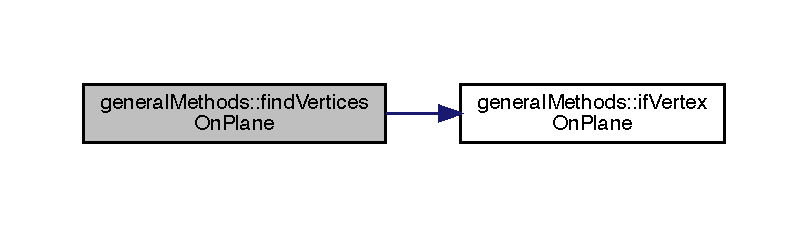
\includegraphics[width=350pt]{namespacegeneral_methods_aa0669678cf59876e3249ddce7a0d1ce3_cgraph}
\end{center}
\end{figure}
Here is the caller graph for this function\+:
\nopagebreak
\begin{figure}[H]
\begin{center}
\leavevmode
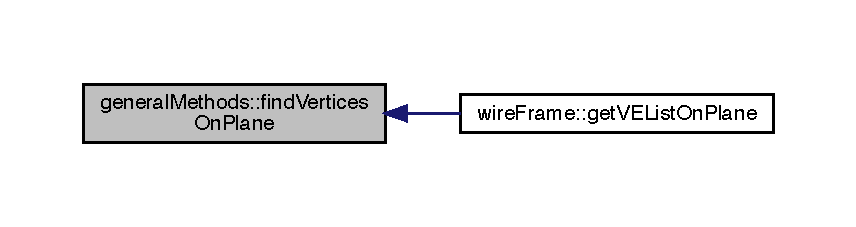
\includegraphics[width=350pt]{namespacegeneral_methods_aa0669678cf59876e3249ddce7a0d1ce3_icgraph}
\end{center}
\end{figure}
\mbox{\Hypertarget{namespacegeneral_methods_a0bd9c59442b6f9c7fd3ae00832ee30df}\label{namespacegeneral_methods_a0bd9c59442b6f9c7fd3ae00832ee30df}} 
\index{general\+Methods@{general\+Methods}!get\+Alpha\+And\+Direction@{get\+Alpha\+And\+Direction}}
\index{get\+Alpha\+And\+Direction@{get\+Alpha\+And\+Direction}!general\+Methods@{general\+Methods}}
\subsubsection{\texorpdfstring{get\+Alpha\+And\+Direction()}{getAlphaAndDirection()}}
{\footnotesize\ttfamily float $\ast$ general\+Methods\+::get\+Alpha\+And\+Direction (\begin{DoxyParamCaption}\item[{\mbox{\hyperlink{classface_loop}{face\+Loop}}}]{flk,  }\item[{\mbox{\hyperlink{classface_loop}{face\+Loop}}}]{fls,  }\item[{\mbox{\hyperlink{structedge3_d}{edge3D}}}]{reference\+Edge }\end{DoxyParamCaption})}

returns alpha as described in paper and whether to select +\+Fs or -\/\+Fs 

Definition at line 417 of file general\+Methods.\+cpp.

Here is the call graph for this function\+:
\nopagebreak
\begin{figure}[H]
\begin{center}
\leavevmode
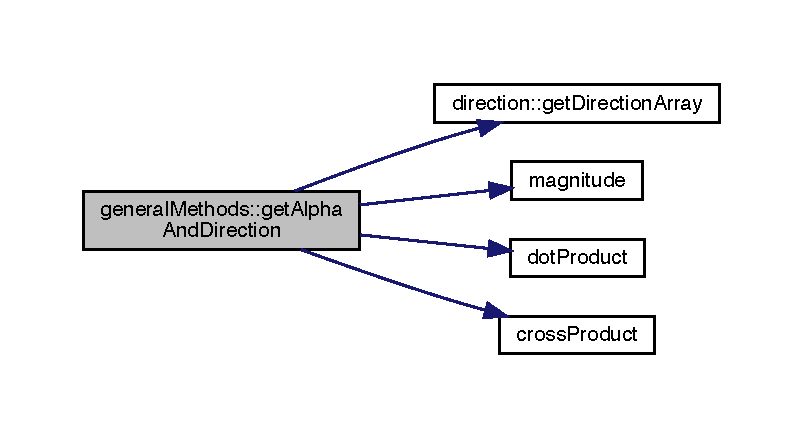
\includegraphics[width=350pt]{namespacegeneral_methods_a0bd9c59442b6f9c7fd3ae00832ee30df_cgraph}
\end{center}
\end{figure}
\mbox{\Hypertarget{namespacegeneral_methods_a4ebb8d563530558e025b62c647045efe}\label{namespacegeneral_methods_a4ebb8d563530558e025b62c647045efe}} 
\index{general\+Methods@{general\+Methods}!get\+If\+Outer@{get\+If\+Outer}}
\index{get\+If\+Outer@{get\+If\+Outer}!general\+Methods@{general\+Methods}}
\subsubsection{\texorpdfstring{get\+If\+Outer()}{getIfOuter()}}
{\footnotesize\ttfamily bool general\+Methods\+::get\+If\+Outer (\begin{DoxyParamCaption}\item[{\mbox{\hyperlink{classbody_loop}{body\+Loop}}}]{b }\end{DoxyParamCaption})}

to determine whether the bodyloop is outer or inner by the method described in paper \mbox{\Hypertarget{namespacegeneral_methods_afe4087e253b318326a0a1578d34b42ca}\label{namespacegeneral_methods_afe4087e253b318326a0a1578d34b42ca}} 
\index{general\+Methods@{general\+Methods}!get\+Reversed\+Face\+Loop@{get\+Reversed\+Face\+Loop}}
\index{get\+Reversed\+Face\+Loop@{get\+Reversed\+Face\+Loop}!general\+Methods@{general\+Methods}}
\subsubsection{\texorpdfstring{get\+Reversed\+Face\+Loop()}{getReversedFaceLoop()}}
{\footnotesize\ttfamily \mbox{\hyperlink{classface_loop}{face\+Loop}} general\+Methods\+::get\+Reversed\+Face\+Loop (\begin{DoxyParamCaption}\item[{\mbox{\hyperlink{classface_loop}{face\+Loop}}}]{faceloop }\end{DoxyParamCaption})}



Definition at line 474 of file general\+Methods.\+cpp.

Here is the call graph for this function\+:
\nopagebreak
\begin{figure}[H]
\begin{center}
\leavevmode
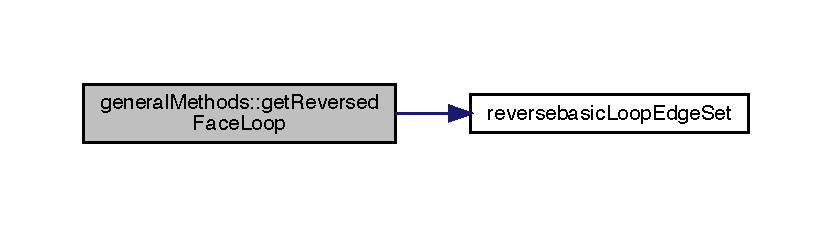
\includegraphics[width=350pt]{namespacegeneral_methods_afe4087e253b318326a0a1578d34b42ca_cgraph}
\end{center}
\end{figure}
Here is the caller graph for this function\+:
\nopagebreak
\begin{figure}[H]
\begin{center}
\leavevmode
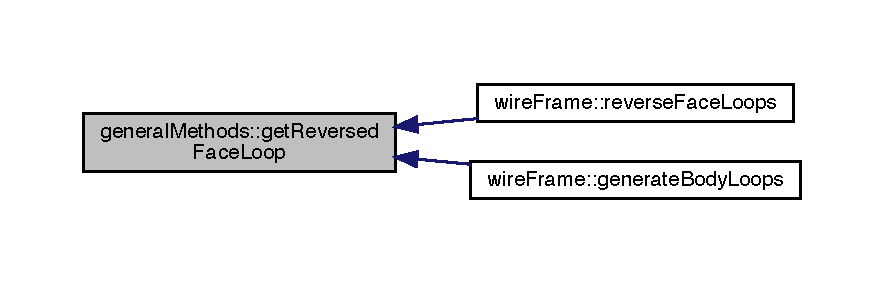
\includegraphics[width=350pt]{namespacegeneral_methods_afe4087e253b318326a0a1578d34b42ca_icgraph}
\end{center}
\end{figure}
\mbox{\Hypertarget{namespacegeneral_methods_a21d2e8c181e8cac3762d9ca1871d2168}\label{namespacegeneral_methods_a21d2e8c181e8cac3762d9ca1871d2168}} 
\index{general\+Methods@{general\+Methods}!if\+Edge\+On\+Plane@{if\+Edge\+On\+Plane}}
\index{if\+Edge\+On\+Plane@{if\+Edge\+On\+Plane}!general\+Methods@{general\+Methods}}
\subsubsection{\texorpdfstring{if\+Edge\+On\+Plane()}{ifEdgeOnPlane()}}
{\footnotesize\ttfamily bool general\+Methods\+::if\+Edge\+On\+Plane (\begin{DoxyParamCaption}\item[{\mbox{\hyperlink{structplane}{plane}}}]{p,  }\item[{\mbox{\hyperlink{structedge3_d}{edge3D}}}]{e }\end{DoxyParamCaption})}

returns distance between a edge and a plane 

Definition at line 221 of file general\+Methods.\+cpp.

Here is the call graph for this function\+:
\nopagebreak
\begin{figure}[H]
\begin{center}
\leavevmode
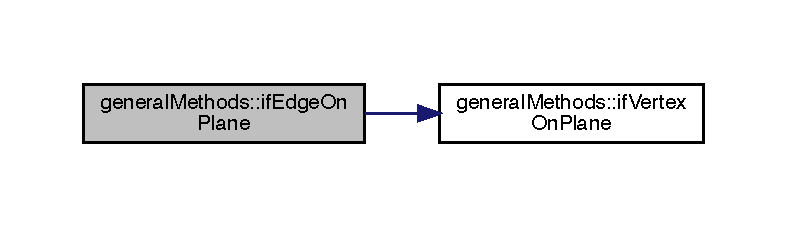
\includegraphics[width=350pt]{namespacegeneral_methods_a21d2e8c181e8cac3762d9ca1871d2168_cgraph}
\end{center}
\end{figure}
Here is the caller graph for this function\+:
\nopagebreak
\begin{figure}[H]
\begin{center}
\leavevmode
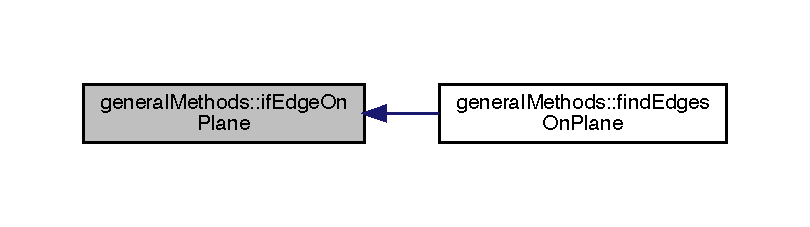
\includegraphics[width=350pt]{namespacegeneral_methods_a21d2e8c181e8cac3762d9ca1871d2168_icgraph}
\end{center}
\end{figure}
\mbox{\Hypertarget{namespacegeneral_methods_a330682bb45234d8de5228a7607d493d2}\label{namespacegeneral_methods_a330682bb45234d8de5228a7607d493d2}} 
\index{general\+Methods@{general\+Methods}!if\+Vertex\+On\+Plane@{if\+Vertex\+On\+Plane}}
\index{if\+Vertex\+On\+Plane@{if\+Vertex\+On\+Plane}!general\+Methods@{general\+Methods}}
\subsubsection{\texorpdfstring{if\+Vertex\+On\+Plane()}{ifVertexOnPlane()}}
{\footnotesize\ttfamily bool general\+Methods\+::if\+Vertex\+On\+Plane (\begin{DoxyParamCaption}\item[{\mbox{\hyperlink{structplane}{plane}}}]{p,  }\item[{\mbox{\hyperlink{structvertex3_d}{vertex3D}}}]{v }\end{DoxyParamCaption})}



Definition at line 215 of file general\+Methods.\+cpp.

Here is the caller graph for this function\+:
\nopagebreak
\begin{figure}[H]
\begin{center}
\leavevmode
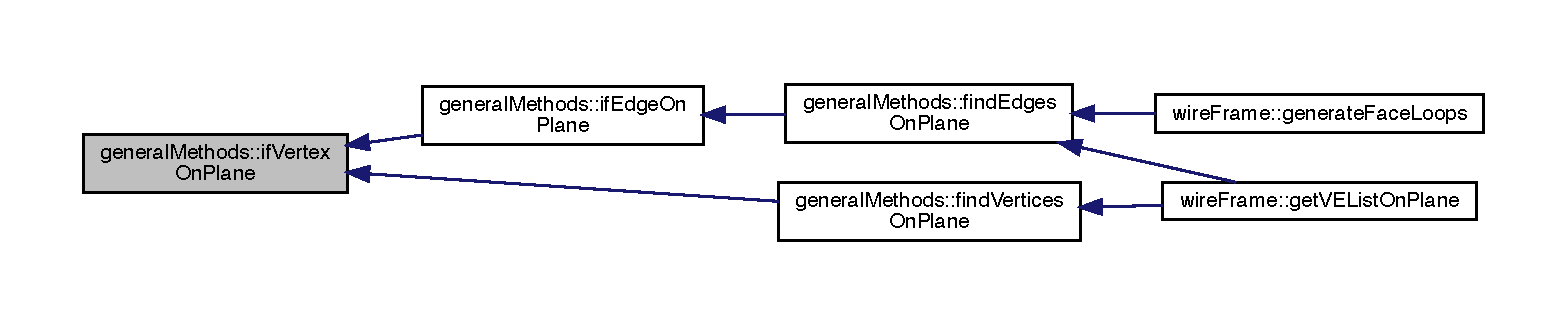
\includegraphics[width=350pt]{namespacegeneral_methods_a330682bb45234d8de5228a7607d493d2_icgraph}
\end{center}
\end{figure}
\mbox{\Hypertarget{namespacegeneral_methods_a27b7ed292415027c495942147e8856b7}\label{namespacegeneral_methods_a27b7ed292415027c495942147e8856b7}} 
\index{general\+Methods@{general\+Methods}!is\+Inside@{is\+Inside}}
\index{is\+Inside@{is\+Inside}!general\+Methods@{general\+Methods}}
\subsubsection{\texorpdfstring{is\+Inside()}{isInside()}}
{\footnotesize\ttfamily bool general\+Methods\+::is\+Inside (\begin{DoxyParamCaption}\item[{std\+::vector$<$ \mbox{\hyperlink{structvertex3_d}{vertex3D}} $>$}]{polygon,  }\item[{int}]{n,  }\item[{\mbox{\hyperlink{structvertex3_d}{vertex3D}}}]{p,  }\item[{\mbox{\hyperlink{structedge3_d}{edge3D}}}]{ref\+Edge,  }\item[{\mbox{\hyperlink{structplane}{plane}}}]{q }\end{DoxyParamCaption})}



Definition at line 323 of file general\+Methods.\+cpp.

Here is the call graph for this function\+:
\nopagebreak
\begin{figure}[H]
\begin{center}
\leavevmode
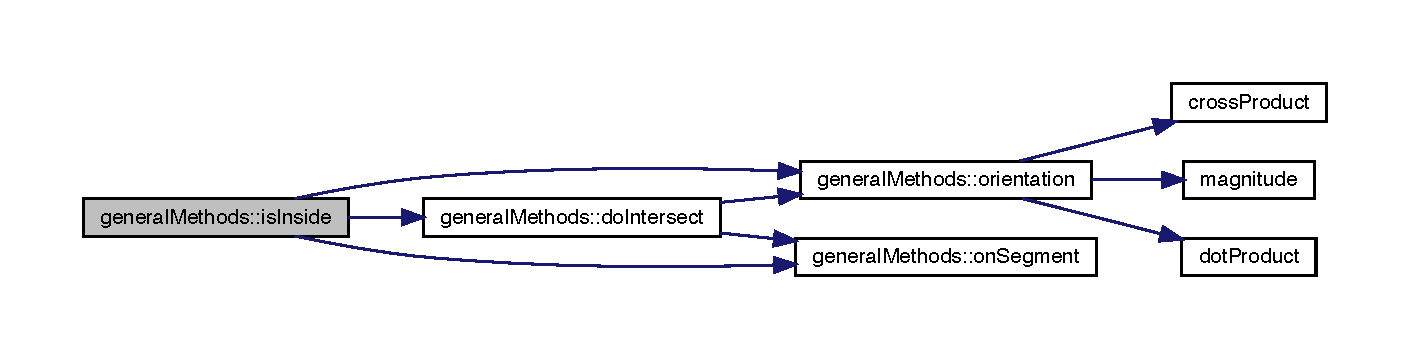
\includegraphics[width=350pt]{namespacegeneral_methods_a27b7ed292415027c495942147e8856b7_cgraph}
\end{center}
\end{figure}
Here is the caller graph for this function\+:
\nopagebreak
\begin{figure}[H]
\begin{center}
\leavevmode
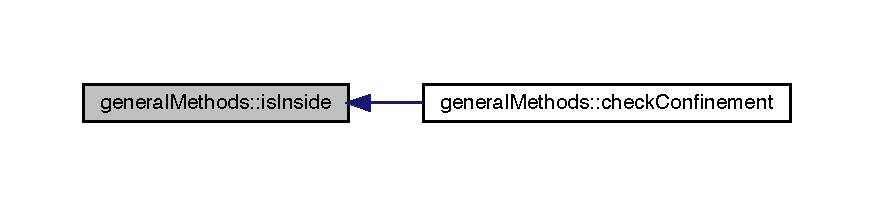
\includegraphics[width=350pt]{namespacegeneral_methods_a27b7ed292415027c495942147e8856b7_icgraph}
\end{center}
\end{figure}
\mbox{\Hypertarget{namespacegeneral_methods_a06d99f1b292d29dbdbe4734847c8d2ee}\label{namespacegeneral_methods_a06d99f1b292d29dbdbe4734847c8d2ee}} 
\index{general\+Methods@{general\+Methods}!make\+Plane@{make\+Plane}}
\index{make\+Plane@{make\+Plane}!general\+Methods@{general\+Methods}}
\subsubsection{\texorpdfstring{make\+Plane()}{makePlane()}}
{\footnotesize\ttfamily \mbox{\hyperlink{structplane}{plane}} general\+Methods\+::make\+Plane (\begin{DoxyParamCaption}\item[{\mbox{\hyperlink{structedge3_d}{edge3D}}}]{e1,  }\item[{\mbox{\hyperlink{structedge3_d}{edge3D}}}]{e2 }\end{DoxyParamCaption})}

take dot procuct ~\newline
~\newline
~\newline
take cross product ~\newline
~\newline
-\/-\/-\/-\/-\/-\/-\/-\/-\/-\/-\/------methods of planes-\/-\/-\/-\/-\/-\/-\/-\/-\/-\/-\/-\/-\/-\/-\/-\/-\/-\/-\/-\/-\/-\/------ ~\newline
make a plane using two adjacent edges 

Definition at line 175 of file general\+Methods.\+cpp.

Here is the call graph for this function\+:
\nopagebreak
\begin{figure}[H]
\begin{center}
\leavevmode
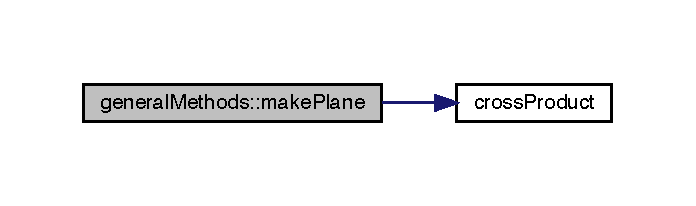
\includegraphics[width=334pt]{namespacegeneral_methods_a06d99f1b292d29dbdbe4734847c8d2ee_cgraph}
\end{center}
\end{figure}
\mbox{\Hypertarget{namespacegeneral_methods_a557bf2257d6658862b42124035aa9588}\label{namespacegeneral_methods_a557bf2257d6658862b42124035aa9588}} 
\index{general\+Methods@{general\+Methods}!on\+Segment@{on\+Segment}}
\index{on\+Segment@{on\+Segment}!general\+Methods@{general\+Methods}}
\subsubsection{\texorpdfstring{on\+Segment()}{onSegment()}}
{\footnotesize\ttfamily bool general\+Methods\+::on\+Segment (\begin{DoxyParamCaption}\item[{\mbox{\hyperlink{structvertex3_d}{vertex3D}}}]{v,  }\item[{\mbox{\hyperlink{structedge3_d}{edge3D}}}]{edge }\end{DoxyParamCaption})}



Definition at line 268 of file general\+Methods.\+cpp.

Here is the caller graph for this function\+:
\nopagebreak
\begin{figure}[H]
\begin{center}
\leavevmode
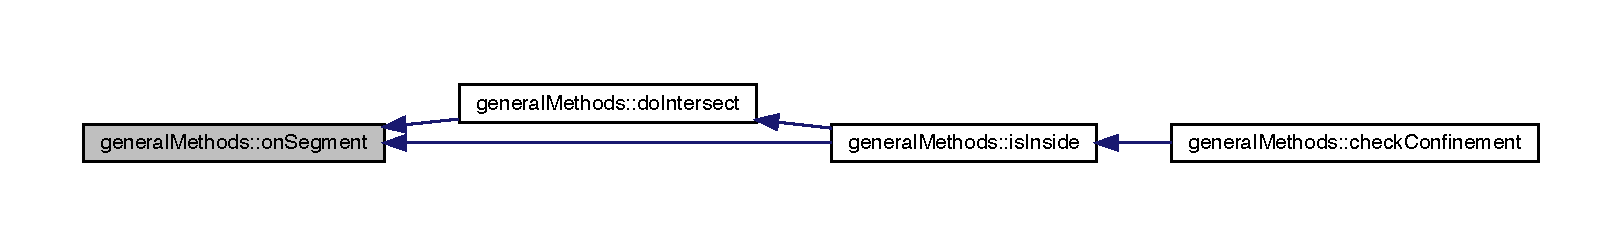
\includegraphics[width=350pt]{namespacegeneral_methods_a557bf2257d6658862b42124035aa9588_icgraph}
\end{center}
\end{figure}
\mbox{\Hypertarget{namespacegeneral_methods_a7bfbfb2a02328d76e70f66fedd57c4ef}\label{namespacegeneral_methods_a7bfbfb2a02328d76e70f66fedd57c4ef}} 
\index{general\+Methods@{general\+Methods}!orientation@{orientation}}
\index{orientation@{orientation}!general\+Methods@{general\+Methods}}
\subsubsection{\texorpdfstring{orientation()}{orientation()}}
{\footnotesize\ttfamily int general\+Methods\+::orientation (\begin{DoxyParamCaption}\item[{\mbox{\hyperlink{structvertex3_d}{vertex3D}}}]{p,  }\item[{\mbox{\hyperlink{structvertex3_d}{vertex3D}}}]{q,  }\item[{\mbox{\hyperlink{structvertex3_d}{vertex3D}}}]{r,  }\item[{\mbox{\hyperlink{structplane}{plane}}}]{s }\end{DoxyParamCaption})}



Definition at line 277 of file general\+Methods.\+cpp.

Here is the call graph for this function\+:
\nopagebreak
\begin{figure}[H]
\begin{center}
\leavevmode
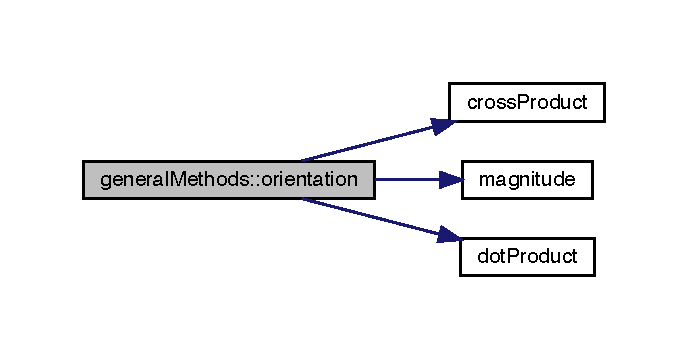
\includegraphics[width=330pt]{namespacegeneral_methods_a7bfbfb2a02328d76e70f66fedd57c4ef_cgraph}
\end{center}
\end{figure}
Here is the caller graph for this function\+:
\nopagebreak
\begin{figure}[H]
\begin{center}
\leavevmode
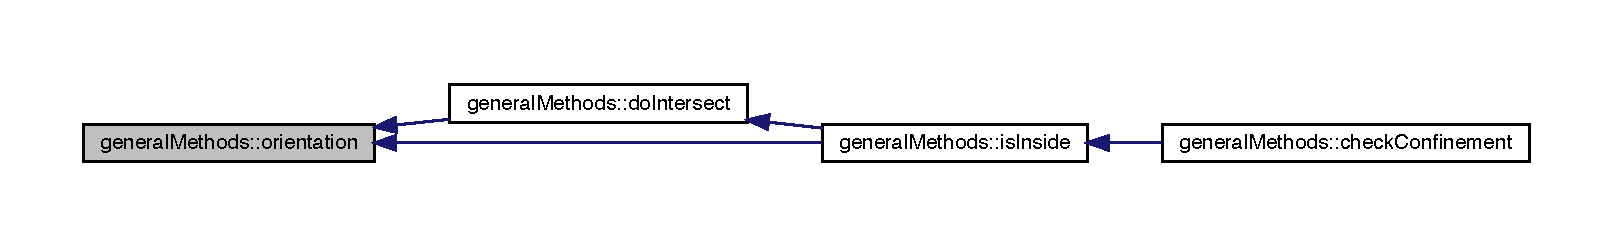
\includegraphics[width=350pt]{namespacegeneral_methods_a7bfbfb2a02328d76e70f66fedd57c4ef_icgraph}
\end{center}
\end{figure}
\mbox{\Hypertarget{namespacegeneral_methods_a3c49599a5ba8f2c41f2ef542bde19765}\label{namespacegeneral_methods_a3c49599a5ba8f2c41f2ef542bde19765}} 
\index{general\+Methods@{general\+Methods}!plane\+Equal@{plane\+Equal}}
\index{plane\+Equal@{plane\+Equal}!general\+Methods@{general\+Methods}}
\subsubsection{\texorpdfstring{plane\+Equal()}{planeEqual()}}
{\footnotesize\ttfamily bool general\+Methods\+::plane\+Equal (\begin{DoxyParamCaption}\item[{\mbox{\hyperlink{structplane}{plane}}}]{p1,  }\item[{\mbox{\hyperlink{structplane}{plane}}}]{p2 }\end{DoxyParamCaption})}



Definition at line 188 of file general\+Methods.\+cpp.

\mbox{\Hypertarget{namespacegeneral_methods_af9a1c28dacf89e746b51916fe178ce1a}\label{namespacegeneral_methods_af9a1c28dacf89e746b51916fe178ce1a}} 
\index{general\+Methods@{general\+Methods}!print\+Edge@{print\+Edge}}
\index{print\+Edge@{print\+Edge}!general\+Methods@{general\+Methods}}
\subsubsection{\texorpdfstring{print\+Edge()}{printEdge()}}
{\footnotesize\ttfamily void general\+Methods\+::print\+Edge (\begin{DoxyParamCaption}\item[{\mbox{\hyperlink{structedge3_d}{edge3D}}}]{i }\end{DoxyParamCaption})}

~\newline
print the edge\+List

~\newline
print the edge\+List

Definition at line 36 of file general\+Methods.\+cpp.

Here is the call graph for this function\+:
\nopagebreak
\begin{figure}[H]
\begin{center}
\leavevmode
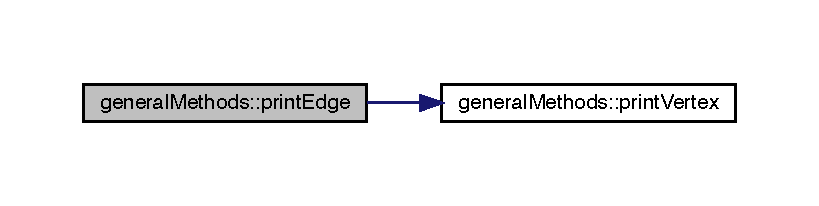
\includegraphics[width=350pt]{namespacegeneral_methods_af9a1c28dacf89e746b51916fe178ce1a_cgraph}
\end{center}
\end{figure}
\mbox{\Hypertarget{namespacegeneral_methods_ab6b6f8a5d92b39ead6c97ec0917b75a4}\label{namespacegeneral_methods_ab6b6f8a5d92b39ead6c97ec0917b75a4}} 
\index{general\+Methods@{general\+Methods}!print\+Edge\+List@{print\+Edge\+List}}
\index{print\+Edge\+List@{print\+Edge\+List}!general\+Methods@{general\+Methods}}
\subsubsection{\texorpdfstring{print\+Edge\+List()}{printEdgeList()}}
{\footnotesize\ttfamily void general\+Methods\+::print\+Edge\+List (\begin{DoxyParamCaption}\item[{vector$<$ \mbox{\hyperlink{structedge3_d}{edge3D}} $>$}]{e }\end{DoxyParamCaption})}

~\newline
print the edge\+List

~\newline
print the edge\+List

Definition at line 43 of file general\+Methods.\+cpp.

Here is the call graph for this function\+:
\nopagebreak
\begin{figure}[H]
\begin{center}
\leavevmode
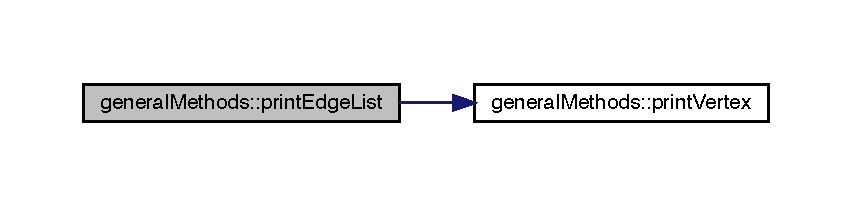
\includegraphics[width=350pt]{namespacegeneral_methods_ab6b6f8a5d92b39ead6c97ec0917b75a4_cgraph}
\end{center}
\end{figure}
Here is the caller graph for this function\+:
\nopagebreak
\begin{figure}[H]
\begin{center}
\leavevmode
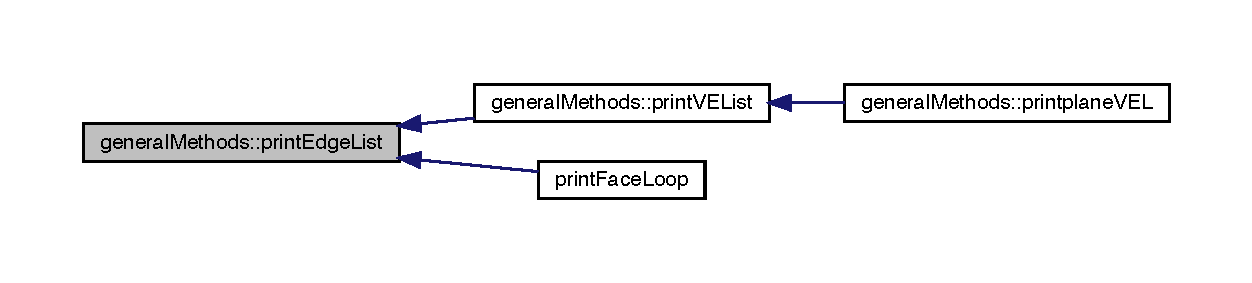
\includegraphics[width=350pt]{namespacegeneral_methods_ab6b6f8a5d92b39ead6c97ec0917b75a4_icgraph}
\end{center}
\end{figure}
\mbox{\Hypertarget{namespacegeneral_methods_a3474d24f9f545407bb5f73250a5e19d7}\label{namespacegeneral_methods_a3474d24f9f545407bb5f73250a5e19d7}} 
\index{general\+Methods@{general\+Methods}!print\+Plane@{print\+Plane}}
\index{print\+Plane@{print\+Plane}!general\+Methods@{general\+Methods}}
\subsubsection{\texorpdfstring{print\+Plane()}{printPlane()}}
{\footnotesize\ttfamily void general\+Methods\+::print\+Plane (\begin{DoxyParamCaption}\item[{\mbox{\hyperlink{structplane}{plane}}}]{p }\end{DoxyParamCaption})}



Definition at line 53 of file general\+Methods.\+cpp.

Here is the caller graph for this function\+:
\nopagebreak
\begin{figure}[H]
\begin{center}
\leavevmode
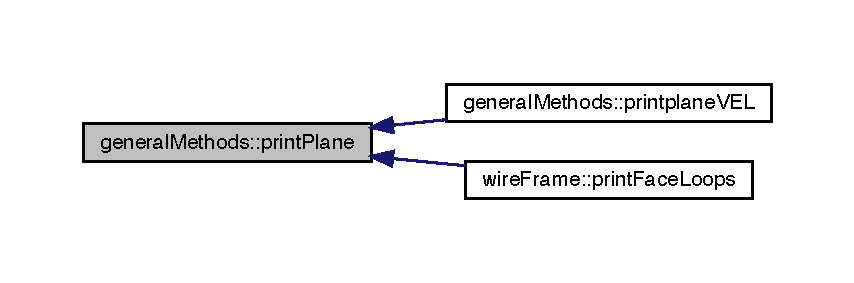
\includegraphics[width=350pt]{namespacegeneral_methods_a3474d24f9f545407bb5f73250a5e19d7_icgraph}
\end{center}
\end{figure}
\mbox{\Hypertarget{namespacegeneral_methods_aa7c9b8abc94ae6b08d2cf083a08eaf21}\label{namespacegeneral_methods_aa7c9b8abc94ae6b08d2cf083a08eaf21}} 
\index{general\+Methods@{general\+Methods}!print\+Planes@{print\+Planes}}
\index{print\+Planes@{print\+Planes}!general\+Methods@{general\+Methods}}
\subsubsection{\texorpdfstring{print\+Planes()}{printPlanes()}}
{\footnotesize\ttfamily void general\+Methods\+::print\+Planes (\begin{DoxyParamCaption}\item[{vector$<$ \mbox{\hyperlink{structplane}{plane}} $>$}]{p }\end{DoxyParamCaption})}



Definition at line 57 of file general\+Methods.\+cpp.

\mbox{\Hypertarget{namespacegeneral_methods_adc8e104a2f2ed35a22be9a68051ec38d}\label{namespacegeneral_methods_adc8e104a2f2ed35a22be9a68051ec38d}} 
\index{general\+Methods@{general\+Methods}!printplane\+V\+EL@{printplane\+V\+EL}}
\index{printplane\+V\+EL@{printplane\+V\+EL}!general\+Methods@{general\+Methods}}
\subsubsection{\texorpdfstring{printplane\+V\+E\+L()}{printplaneVEL()}}
{\footnotesize\ttfamily void general\+Methods\+::printplane\+V\+EL (\begin{DoxyParamCaption}\item[{\mbox{\hyperlink{structplane_v_e_l}{plane\+V\+EL}}}]{p }\end{DoxyParamCaption})}



Definition at line 71 of file general\+Methods.\+cpp.

Here is the call graph for this function\+:
\nopagebreak
\begin{figure}[H]
\begin{center}
\leavevmode
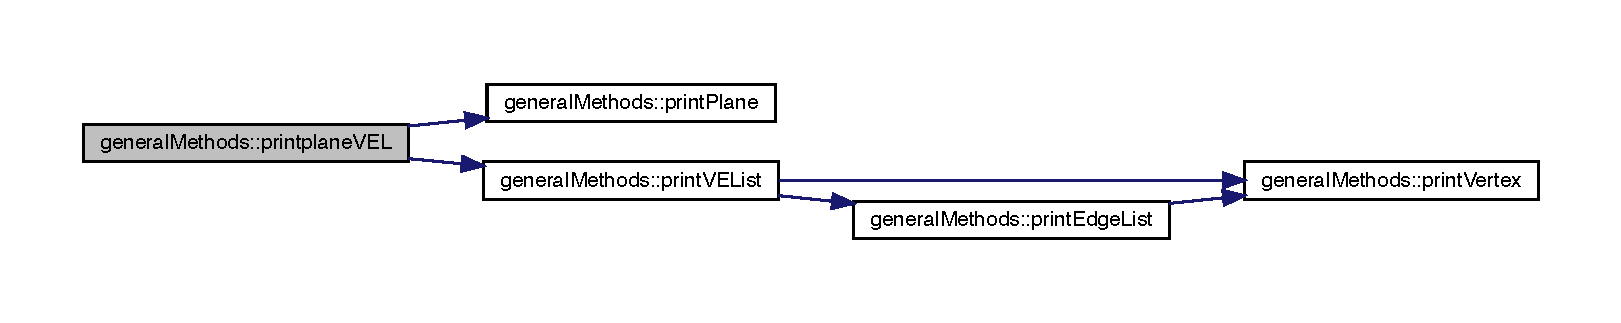
\includegraphics[width=350pt]{namespacegeneral_methods_adc8e104a2f2ed35a22be9a68051ec38d_cgraph}
\end{center}
\end{figure}
\mbox{\Hypertarget{namespacegeneral_methods_a60a9e0ba058824389fc703dc2dbbb7e3}\label{namespacegeneral_methods_a60a9e0ba058824389fc703dc2dbbb7e3}} 
\index{general\+Methods@{general\+Methods}!print\+V\+E\+List@{print\+V\+E\+List}}
\index{print\+V\+E\+List@{print\+V\+E\+List}!general\+Methods@{general\+Methods}}
\subsubsection{\texorpdfstring{print\+V\+E\+List()}{printVEList()}}
{\footnotesize\ttfamily void general\+Methods\+::print\+V\+E\+List (\begin{DoxyParamCaption}\item[{\mbox{\hyperlink{structvertex_edge_list}{vertex\+Edge\+List}}}]{ve\+List }\end{DoxyParamCaption})}



Definition at line 63 of file general\+Methods.\+cpp.

Here is the call graph for this function\+:
\nopagebreak
\begin{figure}[H]
\begin{center}
\leavevmode
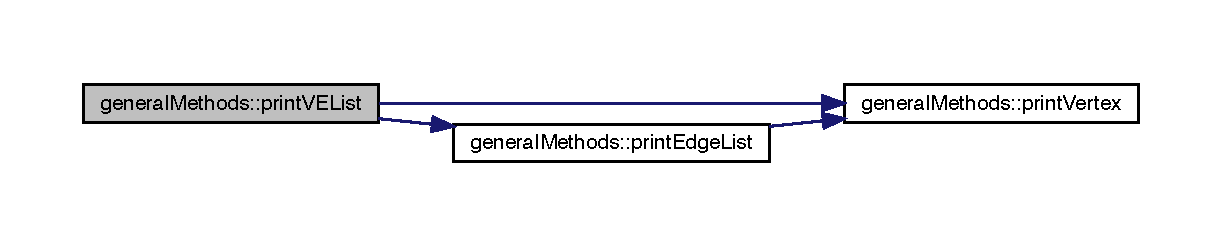
\includegraphics[width=350pt]{namespacegeneral_methods_a60a9e0ba058824389fc703dc2dbbb7e3_cgraph}
\end{center}
\end{figure}
Here is the caller graph for this function\+:
\nopagebreak
\begin{figure}[H]
\begin{center}
\leavevmode
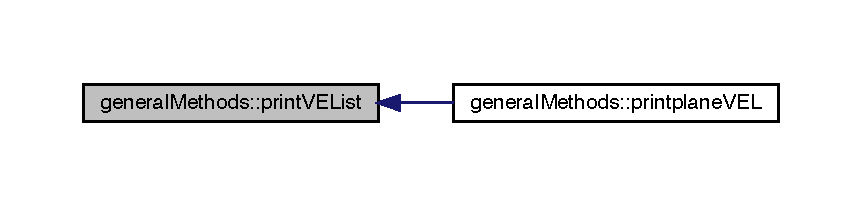
\includegraphics[width=350pt]{namespacegeneral_methods_a60a9e0ba058824389fc703dc2dbbb7e3_icgraph}
\end{center}
\end{figure}
\mbox{\Hypertarget{namespacegeneral_methods_a694306c7472ee1bbfb3c90c0f3d5453a}\label{namespacegeneral_methods_a694306c7472ee1bbfb3c90c0f3d5453a}} 
\index{general\+Methods@{general\+Methods}!print\+Vertex@{print\+Vertex}}
\index{print\+Vertex@{print\+Vertex}!general\+Methods@{general\+Methods}}
\subsubsection{\texorpdfstring{print\+Vertex()}{printVertex()}}
{\footnotesize\ttfamily void general\+Methods\+::print\+Vertex (\begin{DoxyParamCaption}\item[{\mbox{\hyperlink{structvertex3_d}{vertex3D}}}]{i }\end{DoxyParamCaption})}



print methods 

print methods 

Definition at line 20 of file general\+Methods.\+cpp.

Here is the caller graph for this function\+:
\nopagebreak
\begin{figure}[H]
\begin{center}
\leavevmode
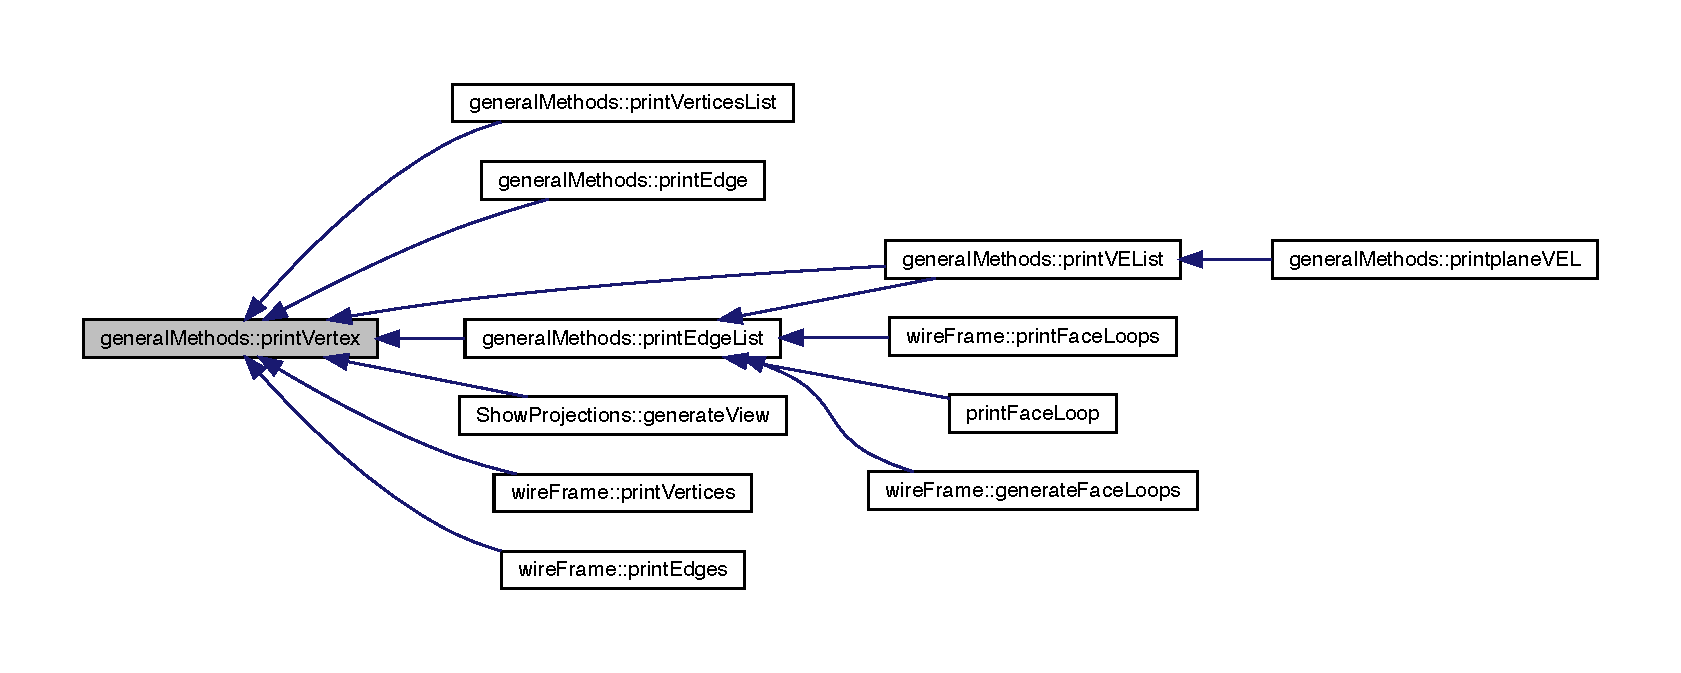
\includegraphics[width=350pt]{namespacegeneral_methods_a694306c7472ee1bbfb3c90c0f3d5453a_icgraph}
\end{center}
\end{figure}
\mbox{\Hypertarget{namespacegeneral_methods_a9cbf7d7c2019f0e2b6f9773b687b50cd}\label{namespacegeneral_methods_a9cbf7d7c2019f0e2b6f9773b687b50cd}} 
\index{general\+Methods@{general\+Methods}!print\+Vertices\+List@{print\+Vertices\+List}}
\index{print\+Vertices\+List@{print\+Vertices\+List}!general\+Methods@{general\+Methods}}
\subsubsection{\texorpdfstring{print\+Vertices\+List()}{printVerticesList()}}
{\footnotesize\ttfamily void general\+Methods\+::print\+Vertices\+List (\begin{DoxyParamCaption}\item[{vector$<$ \mbox{\hyperlink{structvertex3_d}{vertex3D}} $>$}]{v }\end{DoxyParamCaption})}

print the vertex\+List

print the vertex\+List

Definition at line 24 of file general\+Methods.\+cpp.

Here is the call graph for this function\+:
\nopagebreak
\begin{figure}[H]
\begin{center}
\leavevmode
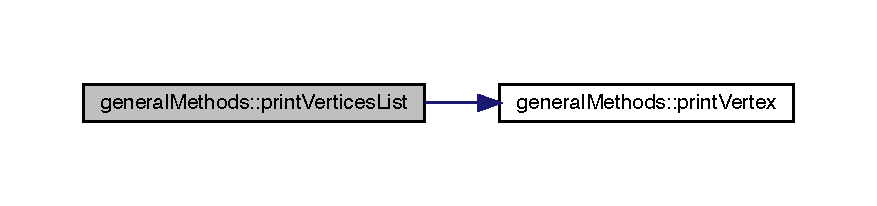
\includegraphics[width=350pt]{namespacegeneral_methods_a9cbf7d7c2019f0e2b6f9773b687b50cd_cgraph}
\end{center}
\end{figure}
\mbox{\Hypertarget{namespacegeneral_methods_a13072e8b14fcea9ae253085569062158}\label{namespacegeneral_methods_a13072e8b14fcea9ae253085569062158}} 
\index{general\+Methods@{general\+Methods}!remove\+Duplicate@{remove\+Duplicate}}
\index{remove\+Duplicate@{remove\+Duplicate}!general\+Methods@{general\+Methods}}
\subsubsection{\texorpdfstring{remove\+Duplicate()}{removeDuplicate()}}
{\footnotesize\ttfamily std\+::vector$<$ \mbox{\hyperlink{structplane}{plane}} $>$ general\+Methods\+::remove\+Duplicate (\begin{DoxyParamCaption}\item[{std\+::vector$<$ \mbox{\hyperlink{structplane}{plane}} $>$}]{v }\end{DoxyParamCaption})}

use this to make all possible planes and then remove the duplicate ones 

Definition at line 195 of file general\+Methods.\+cpp.

\mbox{\Hypertarget{namespacegeneral_methods_ace3487740f3b46dce9e0357366abf9ed}\label{namespacegeneral_methods_ace3487740f3b46dce9e0357366abf9ed}} 
\index{general\+Methods@{general\+Methods}!sort\+Vertices@{sort\+Vertices}}
\index{sort\+Vertices@{sort\+Vertices}!general\+Methods@{general\+Methods}}
\subsubsection{\texorpdfstring{sort\+Vertices()}{sortVertices()}}
{\footnotesize\ttfamily std\+::vector$<$ \mbox{\hyperlink{structvertex3_d}{vertex3D}} $>$ general\+Methods\+::sort\+Vertices (\begin{DoxyParamCaption}\item[{std\+::vector$<$ \mbox{\hyperlink{structvertex3_d}{vertex3D}} $>$}]{V,  }\item[{\mbox{\hyperlink{structedge3_d}{edge3D}}}]{e }\end{DoxyParamCaption})}

-\/-\/-\/-\/-\/-\/-\/-\/-\/-\/-\/------methods of vertices-\/-\/-\/-\/-\/-\/-\/-\/-\/-\/-\/-\/-\/-\/-\/-\/-\/-\/-\/-\/------ ~\newline
sort the vertices along a given edge 

Definition at line 105 of file general\+Methods.\+cpp.

Here is the call graph for this function\+:
\nopagebreak
\begin{figure}[H]
\begin{center}
\leavevmode
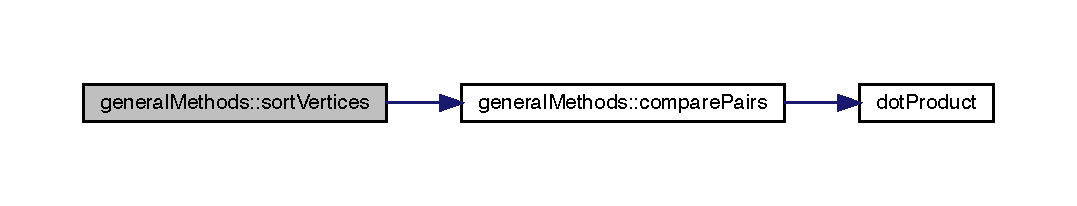
\includegraphics[width=350pt]{namespacegeneral_methods_ace3487740f3b46dce9e0357366abf9ed_cgraph}
\end{center}
\end{figure}
Here is the caller graph for this function\+:
\nopagebreak
\begin{figure}[H]
\begin{center}
\leavevmode
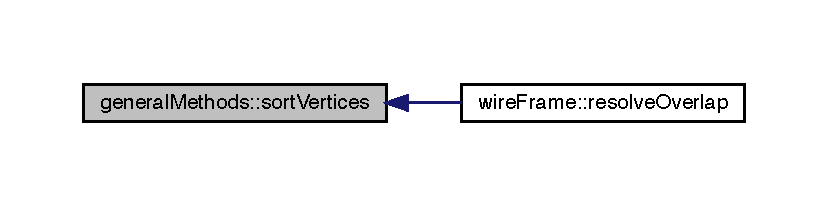
\includegraphics[width=350pt]{namespacegeneral_methods_ace3487740f3b46dce9e0357366abf9ed_icgraph}
\end{center}
\end{figure}

\hypertarget{namespace_ui}{}\section{Ui Namespace Reference}
\label{namespace_ui}\index{Ui@{Ui}}
\subsection*{Classes}
\begin{DoxyCompactItemize}
\item 
class \mbox{\hyperlink{class_ui_1_1_main_window}{Main\+Window}}
\item 
class \mbox{\hyperlink{class_ui_1_1_selection}{Selection}}
\item 
class \mbox{\hyperlink{class_ui_1_1_show_projections}{Show\+Projections}}
\end{DoxyCompactItemize}

\chapter{Class Documentation}
\hypertarget{classbasic_loop_edge_set}{}\section{basic\+Loop\+Edge\+Set Class Reference}
\label{classbasic_loop_edge_set}\index{basic\+Loop\+Edge\+Set@{basic\+Loop\+Edge\+Set}}


{\ttfamily \#include $<$basic\+Loop\+Edge\+Set.\+h$>$}

\subsection*{Public Member Functions}
\begin{DoxyCompactItemize}
\item 
void \mbox{\hyperlink{classbasic_loop_edge_set_a796243033ab3276548e7ff644705dddc}{add\+Edge}} (\mbox{\hyperlink{structedge3_d}{edge3D}} e)
\item 
void \mbox{\hyperlink{classbasic_loop_edge_set_aa58522d2678542f6c50888944f7fea4b}{remove\+Edge}} (\mbox{\hyperlink{structedge3_d}{edge3D}} e)
\item 
void \mbox{\hyperlink{classbasic_loop_edge_set_addb31fe543f58c29b77205f724afb1af}{sort}} ()
\end{DoxyCompactItemize}
\subsection*{Public Attributes}
\begin{DoxyCompactItemize}
\item 
std\+::vector$<$ \mbox{\hyperlink{structedge3_d}{edge3D}} $>$ \mbox{\hyperlink{classbasic_loop_edge_set_a30772bbabe3b0b80f3c3dfe7b7ac8c48}{e\+List}}
\end{DoxyCompactItemize}


\subsection{Detailed Description}
this class contains all the edges in a basic loop 

Definition at line 10 of file basic\+Loop\+Edge\+Set.\+h.



\subsection{Member Function Documentation}
\mbox{\Hypertarget{classbasic_loop_edge_set_a796243033ab3276548e7ff644705dddc}\label{classbasic_loop_edge_set_a796243033ab3276548e7ff644705dddc}} 
\index{basic\+Loop\+Edge\+Set@{basic\+Loop\+Edge\+Set}!add\+Edge@{add\+Edge}}
\index{add\+Edge@{add\+Edge}!basic\+Loop\+Edge\+Set@{basic\+Loop\+Edge\+Set}}
\subsubsection{\texorpdfstring{add\+Edge()}{addEdge()}}
{\footnotesize\ttfamily void basic\+Loop\+Edge\+Set\+::add\+Edge (\begin{DoxyParamCaption}\item[{\mbox{\hyperlink{structedge3_d}{edge3D}}}]{e }\end{DoxyParamCaption})}

methods to add and remove edge from basic loop 

Definition at line 7 of file basic\+Loop\+Edge\+Set.\+cpp.

Here is the caller graph for this function\+:
\nopagebreak
\begin{figure}[H]
\begin{center}
\leavevmode
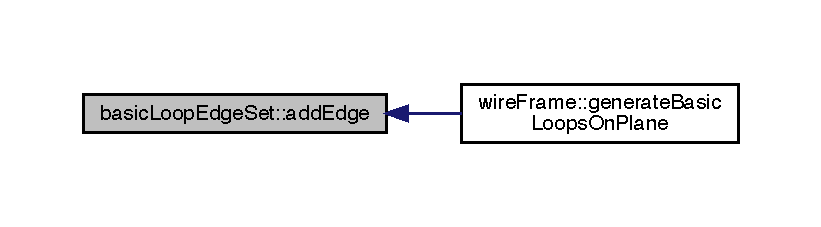
\includegraphics[width=350pt]{classbasic_loop_edge_set_a796243033ab3276548e7ff644705dddc_icgraph}
\end{center}
\end{figure}
\mbox{\Hypertarget{classbasic_loop_edge_set_aa58522d2678542f6c50888944f7fea4b}\label{classbasic_loop_edge_set_aa58522d2678542f6c50888944f7fea4b}} 
\index{basic\+Loop\+Edge\+Set@{basic\+Loop\+Edge\+Set}!remove\+Edge@{remove\+Edge}}
\index{remove\+Edge@{remove\+Edge}!basic\+Loop\+Edge\+Set@{basic\+Loop\+Edge\+Set}}
\subsubsection{\texorpdfstring{remove\+Edge()}{removeEdge()}}
{\footnotesize\ttfamily void basic\+Loop\+Edge\+Set\+::remove\+Edge (\begin{DoxyParamCaption}\item[{\mbox{\hyperlink{structedge3_d}{edge3D}}}]{e }\end{DoxyParamCaption})}



Definition at line 13 of file basic\+Loop\+Edge\+Set.\+cpp.

\mbox{\Hypertarget{classbasic_loop_edge_set_addb31fe543f58c29b77205f724afb1af}\label{classbasic_loop_edge_set_addb31fe543f58c29b77205f724afb1af}} 
\index{basic\+Loop\+Edge\+Set@{basic\+Loop\+Edge\+Set}!sort@{sort}}
\index{sort@{sort}!basic\+Loop\+Edge\+Set@{basic\+Loop\+Edge\+Set}}
\subsubsection{\texorpdfstring{sort()}{sort()}}
{\footnotesize\ttfamily void basic\+Loop\+Edge\+Set\+::sort (\begin{DoxyParamCaption}{ }\end{DoxyParamCaption})}



Definition at line 20 of file basic\+Loop\+Edge\+Set.\+cpp.



\subsection{Member Data Documentation}
\mbox{\Hypertarget{classbasic_loop_edge_set_a30772bbabe3b0b80f3c3dfe7b7ac8c48}\label{classbasic_loop_edge_set_a30772bbabe3b0b80f3c3dfe7b7ac8c48}} 
\index{basic\+Loop\+Edge\+Set@{basic\+Loop\+Edge\+Set}!e\+List@{e\+List}}
\index{e\+List@{e\+List}!basic\+Loop\+Edge\+Set@{basic\+Loop\+Edge\+Set}}
\subsubsection{\texorpdfstring{e\+List}{eList}}
{\footnotesize\ttfamily std\+::vector$<$\mbox{\hyperlink{structedge3_d}{edge3D}}$>$ basic\+Loop\+Edge\+Set\+::e\+List}

all the edges in a basic loop 

Definition at line 16 of file basic\+Loop\+Edge\+Set.\+h.



The documentation for this class was generated from the following files\+:\begin{DoxyCompactItemize}
\item 
include/\mbox{\hyperlink{basic_loop_edge_set_8h}{basic\+Loop\+Edge\+Set.\+h}}\item 
src/\mbox{\hyperlink{basic_loop_edge_set_8cpp}{basic\+Loop\+Edge\+Set.\+cpp}}\end{DoxyCompactItemize}

\hypertarget{classbody_loop}{}\section{body\+Loop Class Reference}
\label{classbody_loop}\index{body\+Loop@{body\+Loop}}


{\ttfamily \#include $<$body\+Loop.\+h$>$}

\subsection*{Public Member Functions}
\begin{DoxyCompactItemize}
\item 
bool \mbox{\hyperlink{classbody_loop_a246832022a7b7008903118462f24e263}{add\+Loop}} (\mbox{\hyperlink{classface_loop}{face\+Loop}} loop)
\item 
void \mbox{\hyperlink{classbody_loop_a963bee3f5118c89183c4eedaa39c3641}{remove\+Loop}} (\mbox{\hyperlink{classface_loop}{face\+Loop}} loop)
\item 
bool \mbox{\hyperlink{classbody_loop_afcbfd878ef953951d47c2564091b9442}{contains\+Loop}} (\mbox{\hyperlink{classface_loop}{face\+Loop}} loop)
\item 
bool \mbox{\hyperlink{classbody_loop_a328d9291b9baae26a01b39d9ff7fbd7d}{legal}} ()
\end{DoxyCompactItemize}
\subsection*{Public Attributes}
\begin{DoxyCompactItemize}
\item 
std\+::vector$<$ \mbox{\hyperlink{classface_loop}{face\+Loop}} $>$ \mbox{\hyperlink{classbody_loop_a44aae842c31a2872e898ee26eaa7cb52}{bodyloop}}
\end{DoxyCompactItemize}


\subsection{Detailed Description}


Definition at line 8 of file body\+Loop.\+h.



\subsection{Member Function Documentation}
\mbox{\Hypertarget{classbody_loop_a246832022a7b7008903118462f24e263}\label{classbody_loop_a246832022a7b7008903118462f24e263}} 
\index{body\+Loop@{body\+Loop}!add\+Loop@{add\+Loop}}
\index{add\+Loop@{add\+Loop}!body\+Loop@{body\+Loop}}
\subsubsection{\texorpdfstring{add\+Loop()}{addLoop()}}
{\footnotesize\ttfamily bool body\+Loop\+::add\+Loop (\begin{DoxyParamCaption}\item[{\mbox{\hyperlink{classface_loop}{face\+Loop}}}]{loop }\end{DoxyParamCaption})}

add loop/remove to face loop 

Definition at line 7 of file body\+Loop.\+cpp.

\mbox{\Hypertarget{classbody_loop_afcbfd878ef953951d47c2564091b9442}\label{classbody_loop_afcbfd878ef953951d47c2564091b9442}} 
\index{body\+Loop@{body\+Loop}!contains\+Loop@{contains\+Loop}}
\index{contains\+Loop@{contains\+Loop}!body\+Loop@{body\+Loop}}
\subsubsection{\texorpdfstring{contains\+Loop()}{containsLoop()}}
{\footnotesize\ttfamily bool body\+Loop\+::contains\+Loop (\begin{DoxyParamCaption}\item[{\mbox{\hyperlink{classface_loop}{face\+Loop}}}]{loop }\end{DoxyParamCaption})}

sets a loop in \mbox{\hyperlink{classbody_loop}{body\+Loop}} as \textquotesingle{}expanded\textquotesingle{} or \textquotesingle{}unexpanded\textquotesingle{} ~\newline
does \mbox{\hyperlink{classbody_loop}{body\+Loop}} contain a \mbox{\hyperlink{classface_loop}{face\+Loop}} 

Definition at line 21 of file body\+Loop.\+cpp.

\mbox{\Hypertarget{classbody_loop_a328d9291b9baae26a01b39d9ff7fbd7d}\label{classbody_loop_a328d9291b9baae26a01b39d9ff7fbd7d}} 
\index{body\+Loop@{body\+Loop}!legal@{legal}}
\index{legal@{legal}!body\+Loop@{body\+Loop}}
\subsubsection{\texorpdfstring{legal()}{legal()}}
{\footnotesize\ttfamily bool body\+Loop\+::legal (\begin{DoxyParamCaption}{ }\end{DoxyParamCaption})}

returns whether bodyloop is legal 

Definition at line 25 of file body\+Loop.\+cpp.

\mbox{\Hypertarget{classbody_loop_a963bee3f5118c89183c4eedaa39c3641}\label{classbody_loop_a963bee3f5118c89183c4eedaa39c3641}} 
\index{body\+Loop@{body\+Loop}!remove\+Loop@{remove\+Loop}}
\index{remove\+Loop@{remove\+Loop}!body\+Loop@{body\+Loop}}
\subsubsection{\texorpdfstring{remove\+Loop()}{removeLoop()}}
{\footnotesize\ttfamily void body\+Loop\+::remove\+Loop (\begin{DoxyParamCaption}\item[{\mbox{\hyperlink{classface_loop}{face\+Loop}}}]{loop }\end{DoxyParamCaption})}



Definition at line 15 of file body\+Loop.\+cpp.



\subsection{Member Data Documentation}
\mbox{\Hypertarget{classbody_loop_a44aae842c31a2872e898ee26eaa7cb52}\label{classbody_loop_a44aae842c31a2872e898ee26eaa7cb52}} 
\index{body\+Loop@{body\+Loop}!bodyloop@{bodyloop}}
\index{bodyloop@{bodyloop}!body\+Loop@{body\+Loop}}
\subsubsection{\texorpdfstring{bodyloop}{bodyloop}}
{\footnotesize\ttfamily std\+::vector$<$\mbox{\hyperlink{classface_loop}{face\+Loop}} $>$ body\+Loop\+::bodyloop}



Definition at line 10 of file body\+Loop.\+h.



The documentation for this class was generated from the following files\+:\begin{DoxyCompactItemize}
\item 
include/\mbox{\hyperlink{body_loop_8h}{body\+Loop.\+h}}\item 
src/\mbox{\hyperlink{body_loop_8cpp}{body\+Loop.\+cpp}}\end{DoxyCompactItemize}

\hypertarget{structdirection}{}\section{direction Struct Reference}
\label{structdirection}\index{direction@{direction}}


{\ttfamily \#include $<$structs.\+h$>$}

\subsection*{Public Member Functions}
\begin{DoxyCompactItemize}
\item 
\mbox{\hyperlink{structdirection_aec63de1bc5de2b04a10ba05ccf5d1e5c}{direction}} ()
\item 
\mbox{\hyperlink{structdirection_aa110e167446e56347dae0ec110acd666}{direction}} (float X, float Y, float Z)
\item 
bool \mbox{\hyperlink{structdirection_a07af488d6fa8d5b140fedf087f6d62d9}{operator==}} (const \mbox{\hyperlink{structdirection}{direction}} \&rhs)
\item 
float $\ast$ \mbox{\hyperlink{structdirection_af1cd0f36bb6f2ed44c2adc4599288b28}{get\+Direction\+Array}} ()
\end{DoxyCompactItemize}
\subsection*{Public Attributes}
\begin{DoxyCompactItemize}
\item 
float \mbox{\hyperlink{structdirection_a19fc7fb15e44643c1816108b180c875c}{x}}
\item 
float \mbox{\hyperlink{structdirection_a8b42de830050ebb6df61e00178677d4a}{y}}
\item 
float \mbox{\hyperlink{structdirection_a417fbafba9a383aaf1bb843e540c5f95}{z}}
\item 
float \mbox{\hyperlink{structdirection_a63c93cc6656f46d483d80a6fbbd2f5b0}{array}} \mbox{[}3\mbox{]}
\end{DoxyCompactItemize}


\subsection{Detailed Description}


Definition at line 206 of file structs.\+h.



\subsection{Constructor \& Destructor Documentation}
\mbox{\Hypertarget{structdirection_aec63de1bc5de2b04a10ba05ccf5d1e5c}\label{structdirection_aec63de1bc5de2b04a10ba05ccf5d1e5c}} 
\index{direction@{direction}!direction@{direction}}
\index{direction@{direction}!direction@{direction}}
\subsubsection{\texorpdfstring{direction()}{direction()}\hspace{0.1cm}{\footnotesize\ttfamily [1/2]}}
{\footnotesize\ttfamily direction\+::direction (\begin{DoxyParamCaption}{ }\end{DoxyParamCaption})\hspace{0.3cm}{\ttfamily [inline]}}



Definition at line 212 of file structs.\+h.

\mbox{\Hypertarget{structdirection_aa110e167446e56347dae0ec110acd666}\label{structdirection_aa110e167446e56347dae0ec110acd666}} 
\index{direction@{direction}!direction@{direction}}
\index{direction@{direction}!direction@{direction}}
\subsubsection{\texorpdfstring{direction()}{direction()}\hspace{0.1cm}{\footnotesize\ttfamily [2/2]}}
{\footnotesize\ttfamily direction\+::direction (\begin{DoxyParamCaption}\item[{float}]{X,  }\item[{float}]{Y,  }\item[{float}]{Z }\end{DoxyParamCaption})\hspace{0.3cm}{\ttfamily [inline]}}



Definition at line 213 of file structs.\+h.



\subsection{Member Function Documentation}
\mbox{\Hypertarget{structdirection_af1cd0f36bb6f2ed44c2adc4599288b28}\label{structdirection_af1cd0f36bb6f2ed44c2adc4599288b28}} 
\index{direction@{direction}!get\+Direction\+Array@{get\+Direction\+Array}}
\index{get\+Direction\+Array@{get\+Direction\+Array}!direction@{direction}}
\subsubsection{\texorpdfstring{get\+Direction\+Array()}{getDirectionArray()}}
{\footnotesize\ttfamily float$\ast$ direction\+::get\+Direction\+Array (\begin{DoxyParamCaption}{ }\end{DoxyParamCaption})\hspace{0.3cm}{\ttfamily [inline]}}



Definition at line 228 of file structs.\+h.

Here is the caller graph for this function\+:
\nopagebreak
\begin{figure}[H]
\begin{center}
\leavevmode
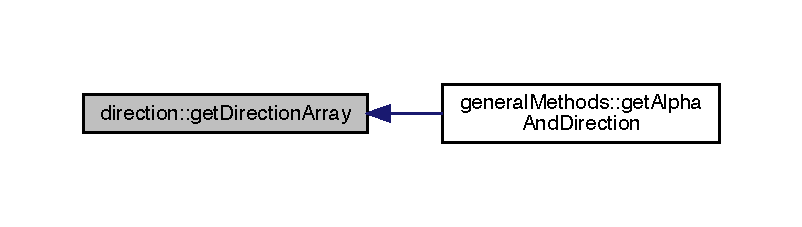
\includegraphics[width=350pt]{structdirection_af1cd0f36bb6f2ed44c2adc4599288b28_icgraph}
\end{center}
\end{figure}
\mbox{\Hypertarget{structdirection_a07af488d6fa8d5b140fedf087f6d62d9}\label{structdirection_a07af488d6fa8d5b140fedf087f6d62d9}} 
\index{direction@{direction}!operator==@{operator==}}
\index{operator==@{operator==}!direction@{direction}}
\subsubsection{\texorpdfstring{operator==()}{operator==()}}
{\footnotesize\ttfamily bool direction\+::operator== (\begin{DoxyParamCaption}\item[{const \mbox{\hyperlink{structdirection}{direction}} \&}]{rhs }\end{DoxyParamCaption})\hspace{0.3cm}{\ttfamily [inline]}}



Definition at line 219 of file structs.\+h.

Here is the call graph for this function\+:
\nopagebreak
\begin{figure}[H]
\begin{center}
\leavevmode
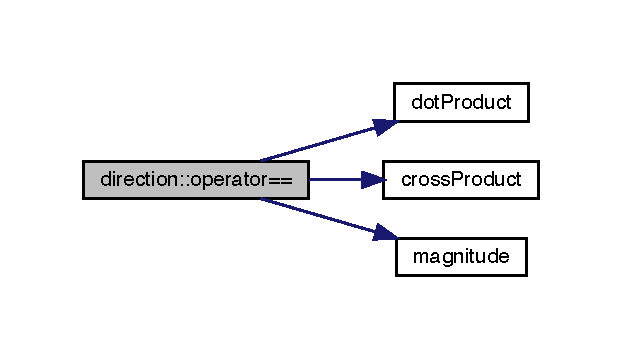
\includegraphics[width=299pt]{structdirection_a07af488d6fa8d5b140fedf087f6d62d9_cgraph}
\end{center}
\end{figure}


\subsection{Member Data Documentation}
\mbox{\Hypertarget{structdirection_a63c93cc6656f46d483d80a6fbbd2f5b0}\label{structdirection_a63c93cc6656f46d483d80a6fbbd2f5b0}} 
\index{direction@{direction}!array@{array}}
\index{array@{array}!direction@{direction}}
\subsubsection{\texorpdfstring{array}{array}}
{\footnotesize\ttfamily float direction\+::array\mbox{[}3\mbox{]}}



Definition at line 211 of file structs.\+h.

\mbox{\Hypertarget{structdirection_a19fc7fb15e44643c1816108b180c875c}\label{structdirection_a19fc7fb15e44643c1816108b180c875c}} 
\index{direction@{direction}!x@{x}}
\index{x@{x}!direction@{direction}}
\subsubsection{\texorpdfstring{x}{x}}
{\footnotesize\ttfamily float direction\+::x}



Definition at line 208 of file structs.\+h.

\mbox{\Hypertarget{structdirection_a8b42de830050ebb6df61e00178677d4a}\label{structdirection_a8b42de830050ebb6df61e00178677d4a}} 
\index{direction@{direction}!y@{y}}
\index{y@{y}!direction@{direction}}
\subsubsection{\texorpdfstring{y}{y}}
{\footnotesize\ttfamily float direction\+::y}



Definition at line 209 of file structs.\+h.

\mbox{\Hypertarget{structdirection_a417fbafba9a383aaf1bb843e540c5f95}\label{structdirection_a417fbafba9a383aaf1bb843e540c5f95}} 
\index{direction@{direction}!z@{z}}
\index{z@{z}!direction@{direction}}
\subsubsection{\texorpdfstring{z}{z}}
{\footnotesize\ttfamily float direction\+::z}



Definition at line 210 of file structs.\+h.



The documentation for this struct was generated from the following file\+:\begin{DoxyCompactItemize}
\item 
include/\mbox{\hyperlink{structs_8h}{structs.\+h}}\end{DoxyCompactItemize}

\hypertarget{structedge2_d}{}\section{edge2D Struct Reference}
\label{structedge2_d}\index{edge2D@{edge2D}}


{\ttfamily \#include $<$structs.\+h$>$}



Collaboration diagram for edge2D\+:
\nopagebreak
\begin{figure}[H]
\begin{center}
\leavevmode
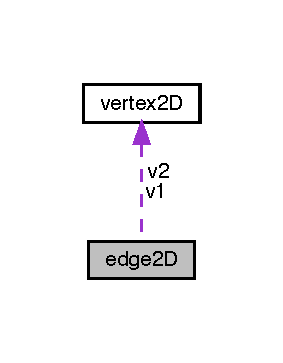
\includegraphics[width=136pt]{structedge2_d__coll__graph}
\end{center}
\end{figure}
\subsection*{Public Member Functions}
\begin{DoxyCompactItemize}
\item 
\mbox{\hyperlink{structedge2_d_abac488760a745ba14a5a0c17693ed3e6}{edge2D}} ()
\item 
\mbox{\hyperlink{structedge2_d_a95676d1bf3e35fbae3ce28a9497c643c}{edge2D}} (\mbox{\hyperlink{structvertex2_d}{vertex2D}} m, \mbox{\hyperlink{structvertex2_d}{vertex2D}} n)
\item 
bool \mbox{\hyperlink{structedge2_d_a305a36218549a8085aca0230ff0cffbc}{operator==}} (const \mbox{\hyperlink{structedge2_d}{edge2D}} \&n)
\item 
void \mbox{\hyperlink{structedge2_d_a5515c7774d5897b9663f2989506023a1}{multiply}} (float scale)
\item 
void \mbox{\hyperlink{structedge2_d_ac22d99c7d0e394a4575b098e79c60ade}{shift}} (float shiftx, float shifty)
\end{DoxyCompactItemize}
\subsection*{Public Attributes}
\begin{DoxyCompactItemize}
\item 
\mbox{\hyperlink{structvertex2_d}{vertex2D}} \mbox{\hyperlink{structedge2_d_ad1d0c2a78bb1b917fc205d94b532111a}{v1}}
\item 
\mbox{\hyperlink{structvertex2_d}{vertex2D}} \mbox{\hyperlink{structedge2_d_ade974e5430928f0a5946820852220717}{v2}}
\item 
bool \mbox{\hyperlink{structedge2_d_a4c16cb9e65f46f54984e53d55ee789b2}{hidden}} = false
\end{DoxyCompactItemize}


\subsection{Detailed Description}
definition of a 2D edge 

Definition at line 52 of file structs.\+h.



\subsection{Constructor \& Destructor Documentation}
\mbox{\Hypertarget{structedge2_d_abac488760a745ba14a5a0c17693ed3e6}\label{structedge2_d_abac488760a745ba14a5a0c17693ed3e6}} 
\index{edge2D@{edge2D}!edge2D@{edge2D}}
\index{edge2D@{edge2D}!edge2D@{edge2D}}
\subsubsection{\texorpdfstring{edge2\+D()}{edge2D()}\hspace{0.1cm}{\footnotesize\ttfamily [1/2]}}
{\footnotesize\ttfamily edge2\+D\+::edge2D (\begin{DoxyParamCaption}{ }\end{DoxyParamCaption})\hspace{0.3cm}{\ttfamily [inline]}}



Definition at line 62 of file structs.\+h.

\mbox{\Hypertarget{structedge2_d_a95676d1bf3e35fbae3ce28a9497c643c}\label{structedge2_d_a95676d1bf3e35fbae3ce28a9497c643c}} 
\index{edge2D@{edge2D}!edge2D@{edge2D}}
\index{edge2D@{edge2D}!edge2D@{edge2D}}
\subsubsection{\texorpdfstring{edge2\+D()}{edge2D()}\hspace{0.1cm}{\footnotesize\ttfamily [2/2]}}
{\footnotesize\ttfamily edge2\+D\+::edge2D (\begin{DoxyParamCaption}\item[{\mbox{\hyperlink{structvertex2_d}{vertex2D}}}]{m,  }\item[{\mbox{\hyperlink{structvertex2_d}{vertex2D}}}]{n }\end{DoxyParamCaption})\hspace{0.3cm}{\ttfamily [inline]}}



Definition at line 65 of file structs.\+h.



\subsection{Member Function Documentation}
\mbox{\Hypertarget{structedge2_d_a5515c7774d5897b9663f2989506023a1}\label{structedge2_d_a5515c7774d5897b9663f2989506023a1}} 
\index{edge2D@{edge2D}!multiply@{multiply}}
\index{multiply@{multiply}!edge2D@{edge2D}}
\subsubsection{\texorpdfstring{multiply()}{multiply()}}
{\footnotesize\ttfamily void edge2\+D\+::multiply (\begin{DoxyParamCaption}\item[{float}]{scale }\end{DoxyParamCaption})\hspace{0.3cm}{\ttfamily [inline]}}



Definition at line 81 of file structs.\+h.

\mbox{\Hypertarget{structedge2_d_a305a36218549a8085aca0230ff0cffbc}\label{structedge2_d_a305a36218549a8085aca0230ff0cffbc}} 
\index{edge2D@{edge2D}!operator==@{operator==}}
\index{operator==@{operator==}!edge2D@{edge2D}}
\subsubsection{\texorpdfstring{operator==()}{operator==()}}
{\footnotesize\ttfamily bool edge2\+D\+::operator== (\begin{DoxyParamCaption}\item[{const \mbox{\hyperlink{structedge2_d}{edge2D}} \&}]{n }\end{DoxyParamCaption})\hspace{0.3cm}{\ttfamily [inline]}}



Definition at line 76 of file structs.\+h.

\mbox{\Hypertarget{structedge2_d_ac22d99c7d0e394a4575b098e79c60ade}\label{structedge2_d_ac22d99c7d0e394a4575b098e79c60ade}} 
\index{edge2D@{edge2D}!shift@{shift}}
\index{shift@{shift}!edge2D@{edge2D}}
\subsubsection{\texorpdfstring{shift()}{shift()}}
{\footnotesize\ttfamily void edge2\+D\+::shift (\begin{DoxyParamCaption}\item[{float}]{shiftx,  }\item[{float}]{shifty }\end{DoxyParamCaption})\hspace{0.3cm}{\ttfamily [inline]}}



Definition at line 87 of file structs.\+h.



\subsection{Member Data Documentation}
\mbox{\Hypertarget{structedge2_d_a4c16cb9e65f46f54984e53d55ee789b2}\label{structedge2_d_a4c16cb9e65f46f54984e53d55ee789b2}} 
\index{edge2D@{edge2D}!hidden@{hidden}}
\index{hidden@{hidden}!edge2D@{edge2D}}
\subsubsection{\texorpdfstring{hidden}{hidden}}
{\footnotesize\ttfamily bool edge2\+D\+::hidden = false}



Definition at line 72 of file structs.\+h.

\mbox{\Hypertarget{structedge2_d_ad1d0c2a78bb1b917fc205d94b532111a}\label{structedge2_d_ad1d0c2a78bb1b917fc205d94b532111a}} 
\index{edge2D@{edge2D}!v1@{v1}}
\index{v1@{v1}!edge2D@{edge2D}}
\subsubsection{\texorpdfstring{v1}{v1}}
{\footnotesize\ttfamily \mbox{\hyperlink{structvertex2_d}{vertex2D}} edge2\+D\+::v1}

end point 1 

Definition at line 56 of file structs.\+h.

\mbox{\Hypertarget{structedge2_d_ade974e5430928f0a5946820852220717}\label{structedge2_d_ade974e5430928f0a5946820852220717}} 
\index{edge2D@{edge2D}!v2@{v2}}
\index{v2@{v2}!edge2D@{edge2D}}
\subsubsection{\texorpdfstring{v2}{v2}}
{\footnotesize\ttfamily \mbox{\hyperlink{structvertex2_d}{vertex2D}} edge2\+D\+::v2}

end point 2 

Definition at line 60 of file structs.\+h.



The documentation for this struct was generated from the following file\+:\begin{DoxyCompactItemize}
\item 
include/\mbox{\hyperlink{structs_8h}{structs.\+h}}\end{DoxyCompactItemize}

\hypertarget{structedge3_d}{}\section{edge3D Struct Reference}
\label{structedge3_d}\index{edge3D@{edge3D}}


{\ttfamily \#include $<$structs.\+h$>$}



Collaboration diagram for edge3D\+:
\nopagebreak
\begin{figure}[H]
\begin{center}
\leavevmode
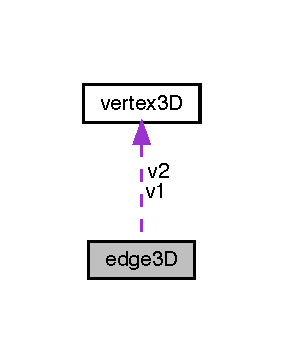
\includegraphics[width=136pt]{structedge3_d__coll__graph}
\end{center}
\end{figure}
\subsection*{Public Member Functions}
\begin{DoxyCompactItemize}
\item 
\mbox{\hyperlink{structedge3_d_a91d257e72d692950510c549e26274cd4}{edge3D}} ()
\item 
\mbox{\hyperlink{structedge3_d_a56bba51f4351182ea95d186db5469671}{edge3D}} (\mbox{\hyperlink{structvertex3_d}{vertex3D}} m, \mbox{\hyperlink{structvertex3_d}{vertex3D}} n)
\item 
bool \mbox{\hyperlink{structedge3_d_a8ef491b6ec193b7fe2c9d4b5e394e964}{operator==}} (const \mbox{\hyperlink{structedge3_d}{edge3D}} \&n)
\end{DoxyCompactItemize}
\subsection*{Public Attributes}
\begin{DoxyCompactItemize}
\item 
\mbox{\hyperlink{structvertex3_d}{vertex3D}} \mbox{\hyperlink{structedge3_d_a3eff6ba2ccba4bfe780a2a7e117f7d1b}{v1}}
\item 
\mbox{\hyperlink{structvertex3_d}{vertex3D}} \mbox{\hyperlink{structedge3_d_a8ed96fe4b567f5bcb861216c96a4081b}{v2}}
\end{DoxyCompactItemize}


\subsection{Detailed Description}
definition of a 3D edge 

Definition at line 137 of file structs.\+h.



\subsection{Constructor \& Destructor Documentation}
\mbox{\Hypertarget{structedge3_d_a91d257e72d692950510c549e26274cd4}\label{structedge3_d_a91d257e72d692950510c549e26274cd4}} 
\index{edge3D@{edge3D}!edge3D@{edge3D}}
\index{edge3D@{edge3D}!edge3D@{edge3D}}
\subsubsection{\texorpdfstring{edge3\+D()}{edge3D()}\hspace{0.1cm}{\footnotesize\ttfamily [1/2]}}
{\footnotesize\ttfamily edge3\+D\+::edge3D (\begin{DoxyParamCaption}{ }\end{DoxyParamCaption})\hspace{0.3cm}{\ttfamily [inline]}}



Definition at line 147 of file structs.\+h.

\mbox{\Hypertarget{structedge3_d_a56bba51f4351182ea95d186db5469671}\label{structedge3_d_a56bba51f4351182ea95d186db5469671}} 
\index{edge3D@{edge3D}!edge3D@{edge3D}}
\index{edge3D@{edge3D}!edge3D@{edge3D}}
\subsubsection{\texorpdfstring{edge3\+D()}{edge3D()}\hspace{0.1cm}{\footnotesize\ttfamily [2/2]}}
{\footnotesize\ttfamily edge3\+D\+::edge3D (\begin{DoxyParamCaption}\item[{\mbox{\hyperlink{structvertex3_d}{vertex3D}}}]{m,  }\item[{\mbox{\hyperlink{structvertex3_d}{vertex3D}}}]{n }\end{DoxyParamCaption})\hspace{0.3cm}{\ttfamily [inline]}}



Definition at line 151 of file structs.\+h.



\subsection{Member Function Documentation}
\mbox{\Hypertarget{structedge3_d_a8ef491b6ec193b7fe2c9d4b5e394e964}\label{structedge3_d_a8ef491b6ec193b7fe2c9d4b5e394e964}} 
\index{edge3D@{edge3D}!operator==@{operator==}}
\index{operator==@{operator==}!edge3D@{edge3D}}
\subsubsection{\texorpdfstring{operator==()}{operator==()}}
{\footnotesize\ttfamily bool edge3\+D\+::operator== (\begin{DoxyParamCaption}\item[{const \mbox{\hyperlink{structedge3_d}{edge3D}} \&}]{n }\end{DoxyParamCaption})\hspace{0.3cm}{\ttfamily [inline]}}



Definition at line 157 of file structs.\+h.



\subsection{Member Data Documentation}
\mbox{\Hypertarget{structedge3_d_a3eff6ba2ccba4bfe780a2a7e117f7d1b}\label{structedge3_d_a3eff6ba2ccba4bfe780a2a7e117f7d1b}} 
\index{edge3D@{edge3D}!v1@{v1}}
\index{v1@{v1}!edge3D@{edge3D}}
\subsubsection{\texorpdfstring{v1}{v1}}
{\footnotesize\ttfamily \mbox{\hyperlink{structvertex3_d}{vertex3D}} edge3\+D\+::v1}

end point 1 

Definition at line 141 of file structs.\+h.

\mbox{\Hypertarget{structedge3_d_a8ed96fe4b567f5bcb861216c96a4081b}\label{structedge3_d_a8ed96fe4b567f5bcb861216c96a4081b}} 
\index{edge3D@{edge3D}!v2@{v2}}
\index{v2@{v2}!edge3D@{edge3D}}
\subsubsection{\texorpdfstring{v2}{v2}}
{\footnotesize\ttfamily \mbox{\hyperlink{structvertex3_d}{vertex3D}} edge3\+D\+::v2}

end point 2 

Definition at line 145 of file structs.\+h.



The documentation for this struct was generated from the following file\+:\begin{DoxyCompactItemize}
\item 
include/\mbox{\hyperlink{structs_8h}{structs.\+h}}\end{DoxyCompactItemize}

\hypertarget{class_edge_list2_d}{}\section{Edge\+List2D Class Reference}
\label{class_edge_list2_d}\index{Edge\+List2D@{Edge\+List2D}}


{\ttfamily \#include $<$Edge\+List2\+D.\+h$>$}

\subsection*{Public Member Functions}
\begin{DoxyCompactItemize}
\item 
void \mbox{\hyperlink{class_edge_list2_d_a0887cfff4dfd1f5c0165750f69f0822a}{add\+Edge}} (\mbox{\hyperlink{structedge2_d}{edge2D}} e)
\begin{DoxyCompactList}\small\item\em add a edge to edge\+List \end{DoxyCompactList}\item 
void \mbox{\hyperlink{class_edge_list2_d_ad0085ac0f30c9135a8193bfef627e57f}{add\+Edge}} (\mbox{\hyperlink{structvertex2_d}{vertex2D}} v1, \mbox{\hyperlink{structvertex2_d}{vertex2D}} v2)
\item 
void \mbox{\hyperlink{class_edge_list2_d_a33ad68f25aa0a9b35af5d983e4effd0b}{remove\+Edge}} (\mbox{\hyperlink{structedge2_d}{edge2D}} e)
\begin{DoxyCompactList}\small\item\em remove a edge from a edge\+List \end{DoxyCompactList}\item 
bool \mbox{\hyperlink{class_edge_list2_d_a9d5ecf2dd50e5f75e189b9588ae784cc}{contains\+Edge}} (\mbox{\hyperlink{structedge2_d}{edge2D}} e)
\end{DoxyCompactItemize}
\subsection*{Public Attributes}
\begin{DoxyCompactItemize}
\item 
vector$<$ \mbox{\hyperlink{structedge2_d}{edge2D}} $>$ \mbox{\hyperlink{class_edge_list2_d_a2e1dfffec9f77e762ecf1aef5b1f428b}{edge\+List}}
\begin{DoxyCompactList}\small\item\em a edge list containing all the edges \end{DoxyCompactList}\end{DoxyCompactItemize}


\subsection{Detailed Description}


Definition at line 6 of file Edge\+List2\+D.\+h.



\subsection{Member Function Documentation}
\mbox{\Hypertarget{class_edge_list2_d_a0887cfff4dfd1f5c0165750f69f0822a}\label{class_edge_list2_d_a0887cfff4dfd1f5c0165750f69f0822a}} 
\index{Edge\+List2D@{Edge\+List2D}!add\+Edge@{add\+Edge}}
\index{add\+Edge@{add\+Edge}!Edge\+List2D@{Edge\+List2D}}
\subsubsection{\texorpdfstring{add\+Edge()}{addEdge()}\hspace{0.1cm}{\footnotesize\ttfamily [1/2]}}
{\footnotesize\ttfamily void Edge\+List2\+D\+::add\+Edge (\begin{DoxyParamCaption}\item[{\mbox{\hyperlink{structedge2_d}{edge2D}}}]{e }\end{DoxyParamCaption})}



add a edge to edge\+List 



Definition at line 7 of file Edge\+List2\+D.\+cpp.

Here is the caller graph for this function\+:
\nopagebreak
\begin{figure}[H]
\begin{center}
\leavevmode
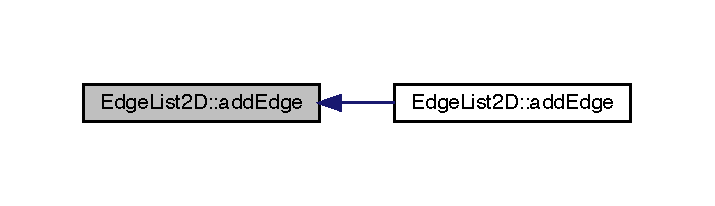
\includegraphics[width=343pt]{class_edge_list2_d_a0887cfff4dfd1f5c0165750f69f0822a_icgraph}
\end{center}
\end{figure}
\mbox{\Hypertarget{class_edge_list2_d_ad0085ac0f30c9135a8193bfef627e57f}\label{class_edge_list2_d_ad0085ac0f30c9135a8193bfef627e57f}} 
\index{Edge\+List2D@{Edge\+List2D}!add\+Edge@{add\+Edge}}
\index{add\+Edge@{add\+Edge}!Edge\+List2D@{Edge\+List2D}}
\subsubsection{\texorpdfstring{add\+Edge()}{addEdge()}\hspace{0.1cm}{\footnotesize\ttfamily [2/2]}}
{\footnotesize\ttfamily void Edge\+List2\+D\+::add\+Edge (\begin{DoxyParamCaption}\item[{\mbox{\hyperlink{structvertex2_d}{vertex2D}}}]{v1,  }\item[{\mbox{\hyperlink{structvertex2_d}{vertex2D}}}]{v2 }\end{DoxyParamCaption})}



Definition at line 14 of file Edge\+List2\+D.\+cpp.

Here is the call graph for this function\+:
\nopagebreak
\begin{figure}[H]
\begin{center}
\leavevmode
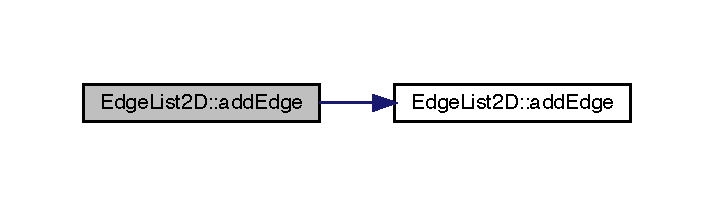
\includegraphics[width=343pt]{class_edge_list2_d_ad0085ac0f30c9135a8193bfef627e57f_cgraph}
\end{center}
\end{figure}
\mbox{\Hypertarget{class_edge_list2_d_a9d5ecf2dd50e5f75e189b9588ae784cc}\label{class_edge_list2_d_a9d5ecf2dd50e5f75e189b9588ae784cc}} 
\index{Edge\+List2D@{Edge\+List2D}!contains\+Edge@{contains\+Edge}}
\index{contains\+Edge@{contains\+Edge}!Edge\+List2D@{Edge\+List2D}}
\subsubsection{\texorpdfstring{contains\+Edge()}{containsEdge()}}
{\footnotesize\ttfamily bool Edge\+List2\+D\+::contains\+Edge (\begin{DoxyParamCaption}\item[{\mbox{\hyperlink{structedge2_d}{edge2D}}}]{e }\end{DoxyParamCaption})}



Definition at line 28 of file Edge\+List2\+D.\+cpp.

Here is the caller graph for this function\+:
\nopagebreak
\begin{figure}[H]
\begin{center}
\leavevmode
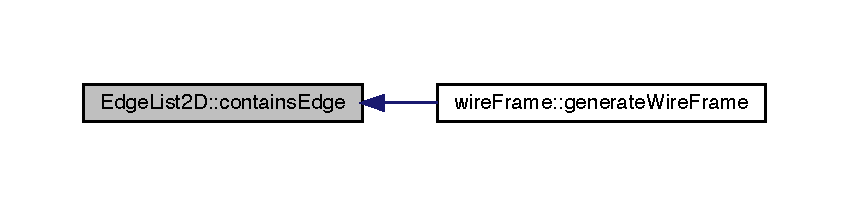
\includegraphics[width=350pt]{class_edge_list2_d_a9d5ecf2dd50e5f75e189b9588ae784cc_icgraph}
\end{center}
\end{figure}
\mbox{\Hypertarget{class_edge_list2_d_a33ad68f25aa0a9b35af5d983e4effd0b}\label{class_edge_list2_d_a33ad68f25aa0a9b35af5d983e4effd0b}} 
\index{Edge\+List2D@{Edge\+List2D}!remove\+Edge@{remove\+Edge}}
\index{remove\+Edge@{remove\+Edge}!Edge\+List2D@{Edge\+List2D}}
\subsubsection{\texorpdfstring{remove\+Edge()}{removeEdge()}}
{\footnotesize\ttfamily void Edge\+List2\+D\+::remove\+Edge (\begin{DoxyParamCaption}\item[{\mbox{\hyperlink{structedge2_d}{edge2D}}}]{e }\end{DoxyParamCaption})}



remove a edge from a edge\+List 



Definition at line 19 of file Edge\+List2\+D.\+cpp.



\subsection{Member Data Documentation}
\mbox{\Hypertarget{class_edge_list2_d_a2e1dfffec9f77e762ecf1aef5b1f428b}\label{class_edge_list2_d_a2e1dfffec9f77e762ecf1aef5b1f428b}} 
\index{Edge\+List2D@{Edge\+List2D}!edge\+List@{edge\+List}}
\index{edge\+List@{edge\+List}!Edge\+List2D@{Edge\+List2D}}
\subsubsection{\texorpdfstring{edge\+List}{edgeList}}
{\footnotesize\ttfamily vector$<$\mbox{\hyperlink{structedge2_d}{edge2D}}$>$ Edge\+List2\+D\+::edge\+List}



a edge list containing all the edges 



Definition at line 10 of file Edge\+List2\+D.\+h.



The documentation for this class was generated from the following files\+:\begin{DoxyCompactItemize}
\item 
include/\mbox{\hyperlink{_edge_list2_d_8h}{Edge\+List2\+D.\+h}}\item 
src/\mbox{\hyperlink{_edge_list2_d_8cpp}{Edge\+List2\+D.\+cpp}}\end{DoxyCompactItemize}

\hypertarget{structedge_vertex_triplet}{}\section{edge\+Vertex\+Triplet Struct Reference}
\label{structedge_vertex_triplet}\index{edge\+Vertex\+Triplet@{edge\+Vertex\+Triplet}}


{\ttfamily \#include $<$structs.\+h$>$}



Collaboration diagram for edge\+Vertex\+Triplet\+:
\nopagebreak
\begin{figure}[H]
\begin{center}
\leavevmode
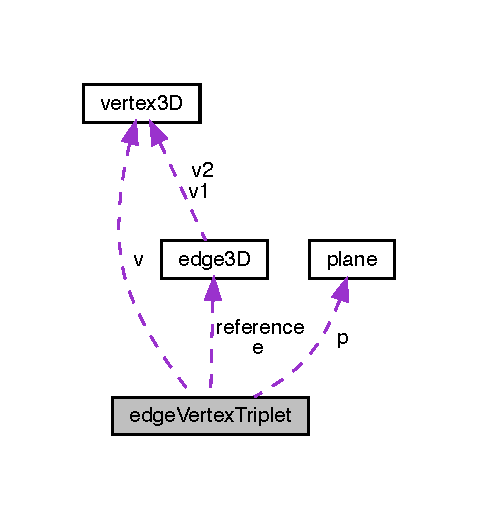
\includegraphics[width=229pt]{structedge_vertex_triplet__coll__graph}
\end{center}
\end{figure}
\subsection*{Public Member Functions}
\begin{DoxyCompactItemize}
\item 
\mbox{\hyperlink{structedge_vertex_triplet_a794c00faebfea5c0bc0b44d7f1e7650c}{edge\+Vertex\+Triplet}} ()
\item 
\mbox{\hyperlink{structedge_vertex_triplet_a50dd657c672509d29a3dff67559c8f6b}{edge\+Vertex\+Triplet}} (\mbox{\hyperlink{structvertex3_d}{vertex3D}} vertex, \mbox{\hyperlink{structedge3_d}{edge3D}} edge, \mbox{\hyperlink{structedge3_d}{edge3D}} r, \mbox{\hyperlink{structplane}{plane}} pln)
\end{DoxyCompactItemize}
\subsection*{Public Attributes}
\begin{DoxyCompactItemize}
\item 
\mbox{\hyperlink{structvertex3_d}{vertex3D}} \mbox{\hyperlink{structedge_vertex_triplet_aae5ca347902fd66a83bf45def3566692}{v}}
\item 
\mbox{\hyperlink{structedge3_d}{edge3D}} \mbox{\hyperlink{structedge_vertex_triplet_a9ccfd63a20315a1aebb2c4d873e3c045}{e}}
\item 
\mbox{\hyperlink{structedge3_d}{edge3D}} \mbox{\hyperlink{structedge_vertex_triplet_afe218b97c39b18b49d4c4e06e937a98f}{reference}}
\item 
\mbox{\hyperlink{structplane}{plane}} \mbox{\hyperlink{structedge_vertex_triplet_a6d523c5de722cb420c3515594be8fc0e}{p}}
\end{DoxyCompactItemize}


\subsection{Detailed Description}


Definition at line 247 of file structs.\+h.



\subsection{Constructor \& Destructor Documentation}
\mbox{\Hypertarget{structedge_vertex_triplet_a794c00faebfea5c0bc0b44d7f1e7650c}\label{structedge_vertex_triplet_a794c00faebfea5c0bc0b44d7f1e7650c}} 
\index{edge\+Vertex\+Triplet@{edge\+Vertex\+Triplet}!edge\+Vertex\+Triplet@{edge\+Vertex\+Triplet}}
\index{edge\+Vertex\+Triplet@{edge\+Vertex\+Triplet}!edge\+Vertex\+Triplet@{edge\+Vertex\+Triplet}}
\subsubsection{\texorpdfstring{edge\+Vertex\+Triplet()}{edgeVertexTriplet()}\hspace{0.1cm}{\footnotesize\ttfamily [1/2]}}
{\footnotesize\ttfamily edge\+Vertex\+Triplet\+::edge\+Vertex\+Triplet (\begin{DoxyParamCaption}{ }\end{DoxyParamCaption})\hspace{0.3cm}{\ttfamily [inline]}}



Definition at line 253 of file structs.\+h.

\mbox{\Hypertarget{structedge_vertex_triplet_a50dd657c672509d29a3dff67559c8f6b}\label{structedge_vertex_triplet_a50dd657c672509d29a3dff67559c8f6b}} 
\index{edge\+Vertex\+Triplet@{edge\+Vertex\+Triplet}!edge\+Vertex\+Triplet@{edge\+Vertex\+Triplet}}
\index{edge\+Vertex\+Triplet@{edge\+Vertex\+Triplet}!edge\+Vertex\+Triplet@{edge\+Vertex\+Triplet}}
\subsubsection{\texorpdfstring{edge\+Vertex\+Triplet()}{edgeVertexTriplet()}\hspace{0.1cm}{\footnotesize\ttfamily [2/2]}}
{\footnotesize\ttfamily edge\+Vertex\+Triplet\+::edge\+Vertex\+Triplet (\begin{DoxyParamCaption}\item[{\mbox{\hyperlink{structvertex3_d}{vertex3D}}}]{vertex,  }\item[{\mbox{\hyperlink{structedge3_d}{edge3D}}}]{edge,  }\item[{\mbox{\hyperlink{structedge3_d}{edge3D}}}]{r,  }\item[{\mbox{\hyperlink{structplane}{plane}}}]{pln }\end{DoxyParamCaption})\hspace{0.3cm}{\ttfamily [inline]}}



Definition at line 254 of file structs.\+h.



\subsection{Member Data Documentation}
\mbox{\Hypertarget{structedge_vertex_triplet_a9ccfd63a20315a1aebb2c4d873e3c045}\label{structedge_vertex_triplet_a9ccfd63a20315a1aebb2c4d873e3c045}} 
\index{edge\+Vertex\+Triplet@{edge\+Vertex\+Triplet}!e@{e}}
\index{e@{e}!edge\+Vertex\+Triplet@{edge\+Vertex\+Triplet}}
\subsubsection{\texorpdfstring{e}{e}}
{\footnotesize\ttfamily \mbox{\hyperlink{structedge3_d}{edge3D}} edge\+Vertex\+Triplet\+::e}



Definition at line 250 of file structs.\+h.

\mbox{\Hypertarget{structedge_vertex_triplet_a6d523c5de722cb420c3515594be8fc0e}\label{structedge_vertex_triplet_a6d523c5de722cb420c3515594be8fc0e}} 
\index{edge\+Vertex\+Triplet@{edge\+Vertex\+Triplet}!p@{p}}
\index{p@{p}!edge\+Vertex\+Triplet@{edge\+Vertex\+Triplet}}
\subsubsection{\texorpdfstring{p}{p}}
{\footnotesize\ttfamily \mbox{\hyperlink{structplane}{plane}} edge\+Vertex\+Triplet\+::p}



Definition at line 252 of file structs.\+h.

\mbox{\Hypertarget{structedge_vertex_triplet_afe218b97c39b18b49d4c4e06e937a98f}\label{structedge_vertex_triplet_afe218b97c39b18b49d4c4e06e937a98f}} 
\index{edge\+Vertex\+Triplet@{edge\+Vertex\+Triplet}!reference@{reference}}
\index{reference@{reference}!edge\+Vertex\+Triplet@{edge\+Vertex\+Triplet}}
\subsubsection{\texorpdfstring{reference}{reference}}
{\footnotesize\ttfamily \mbox{\hyperlink{structedge3_d}{edge3D}} edge\+Vertex\+Triplet\+::reference}



Definition at line 251 of file structs.\+h.

\mbox{\Hypertarget{structedge_vertex_triplet_aae5ca347902fd66a83bf45def3566692}\label{structedge_vertex_triplet_aae5ca347902fd66a83bf45def3566692}} 
\index{edge\+Vertex\+Triplet@{edge\+Vertex\+Triplet}!v@{v}}
\index{v@{v}!edge\+Vertex\+Triplet@{edge\+Vertex\+Triplet}}
\subsubsection{\texorpdfstring{v}{v}}
{\footnotesize\ttfamily \mbox{\hyperlink{structvertex3_d}{vertex3D}} edge\+Vertex\+Triplet\+::v}



Definition at line 249 of file structs.\+h.



The documentation for this struct was generated from the following file\+:\begin{DoxyCompactItemize}
\item 
include/\mbox{\hyperlink{structs_8h}{structs.\+h}}\end{DoxyCompactItemize}

\hypertarget{classface_loop}{}\section{face\+Loop Class Reference}
\label{classface_loop}\index{face\+Loop@{face\+Loop}}


{\ttfamily \#include $<$face\+Loop.\+h$>$}



Collaboration diagram for face\+Loop\+:
\nopagebreak
\begin{figure}[H]
\begin{center}
\leavevmode
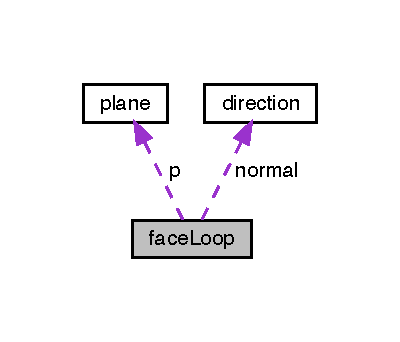
\includegraphics[width=192pt]{classface_loop__coll__graph}
\end{center}
\end{figure}
\subsection*{Public Member Functions}
\begin{DoxyCompactItemize}
\item 
void \mbox{\hyperlink{classface_loop_ae948abd198e6e1496bd320d18b5d638b}{add\+Loop}} (\mbox{\hyperlink{classbasic_loop_edge_set}{basic\+Loop\+Edge\+Set}} loop)
\item 
void \mbox{\hyperlink{classface_loop_ac1c63792b00865fc45ad8934b5580e62}{remove\+Loop}} (\mbox{\hyperlink{classbasic_loop_edge_set}{basic\+Loop\+Edge\+Set}} loop)
\item 
void \mbox{\hyperlink{classface_loop_aa57ee2f9fd011ac4a8aa9b922998c34a}{arrange}} ()
\item 
bool \mbox{\hyperlink{classface_loop_a603c5cfde9765657af9cf088df8fc474}{operator==}} (\mbox{\hyperlink{classface_loop}{face\+Loop}} other) const
\item 
std\+::vector$<$ \mbox{\hyperlink{structedge3_d}{edge3D}} $>$ \mbox{\hyperlink{classface_loop_ad8ba004157748e073c1bc7527fda627c}{get\+All\+Edges}} ()
\item 
bool \mbox{\hyperlink{classface_loop_a3ed69fdb3554a255f484fa78fd1f3361}{if\+Face\+Loop\+Contains}} (\mbox{\hyperlink{structedge3_d}{edge3D}} edge)
\end{DoxyCompactItemize}
\subsection*{Public Attributes}
\begin{DoxyCompactItemize}
\item 
vector$<$ \mbox{\hyperlink{classbasic_loop_edge_set}{basic\+Loop\+Edge\+Set}} $>$ \mbox{\hyperlink{classface_loop_a3f032bc5496c429abc4723632d29ceaf}{faceloop}}
\item 
\mbox{\hyperlink{structdirection}{direction}} \mbox{\hyperlink{classface_loop_a2ac7efac9235e5d6c6c4694f2ea8a6c2}{normal}}
\item 
\mbox{\hyperlink{structplane}{plane}} \mbox{\hyperlink{classface_loop_ace3e113db57081ef98d333a5bfd32daa}{p}}
\end{DoxyCompactItemize}


\subsection{Detailed Description}


Definition at line 17 of file face\+Loop.\+h.



\subsection{Member Function Documentation}
\mbox{\Hypertarget{classface_loop_ae948abd198e6e1496bd320d18b5d638b}\label{classface_loop_ae948abd198e6e1496bd320d18b5d638b}} 
\index{face\+Loop@{face\+Loop}!add\+Loop@{add\+Loop}}
\index{add\+Loop@{add\+Loop}!face\+Loop@{face\+Loop}}
\subsubsection{\texorpdfstring{add\+Loop()}{addLoop()}}
{\footnotesize\ttfamily void face\+Loop\+::add\+Loop (\begin{DoxyParamCaption}\item[{\mbox{\hyperlink{classbasic_loop_edge_set}{basic\+Loop\+Edge\+Set}}}]{loop }\end{DoxyParamCaption})}

add loop to face loop 

Definition at line 8 of file face\+Loop.\+cpp.

\mbox{\Hypertarget{classface_loop_aa57ee2f9fd011ac4a8aa9b922998c34a}\label{classface_loop_aa57ee2f9fd011ac4a8aa9b922998c34a}} 
\index{face\+Loop@{face\+Loop}!arrange@{arrange}}
\index{arrange@{arrange}!face\+Loop@{face\+Loop}}
\subsubsection{\texorpdfstring{arrange()}{arrange()}}
{\footnotesize\ttfamily void face\+Loop\+::arrange (\begin{DoxyParamCaption}{ }\end{DoxyParamCaption})}



Definition at line 48 of file face\+Loop.\+cpp.

Here is the call graph for this function\+:
\nopagebreak
\begin{figure}[H]
\begin{center}
\leavevmode
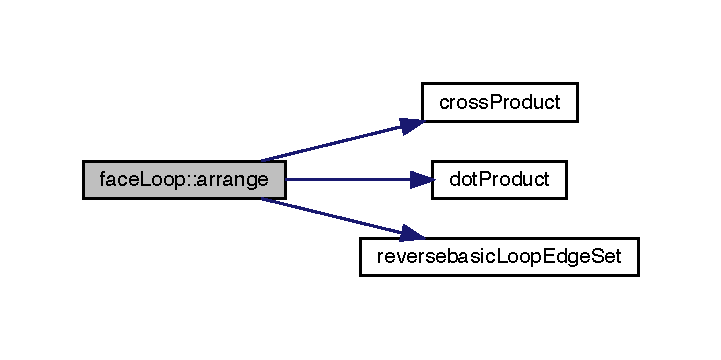
\includegraphics[width=346pt]{classface_loop_aa57ee2f9fd011ac4a8aa9b922998c34a_cgraph}
\end{center}
\end{figure}
Here is the caller graph for this function\+:
\nopagebreak
\begin{figure}[H]
\begin{center}
\leavevmode
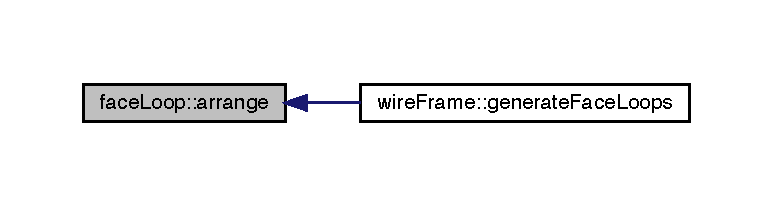
\includegraphics[width=350pt]{classface_loop_aa57ee2f9fd011ac4a8aa9b922998c34a_icgraph}
\end{center}
\end{figure}
\mbox{\Hypertarget{classface_loop_ad8ba004157748e073c1bc7527fda627c}\label{classface_loop_ad8ba004157748e073c1bc7527fda627c}} 
\index{face\+Loop@{face\+Loop}!get\+All\+Edges@{get\+All\+Edges}}
\index{get\+All\+Edges@{get\+All\+Edges}!face\+Loop@{face\+Loop}}
\subsubsection{\texorpdfstring{get\+All\+Edges()}{getAllEdges()}}
{\footnotesize\ttfamily std\+::vector$<$ \mbox{\hyperlink{structedge3_d}{edge3D}} $>$ face\+Loop\+::get\+All\+Edges (\begin{DoxyParamCaption}{ }\end{DoxyParamCaption})}



Definition at line 124 of file face\+Loop.\+cpp.

\mbox{\Hypertarget{classface_loop_a3ed69fdb3554a255f484fa78fd1f3361}\label{classface_loop_a3ed69fdb3554a255f484fa78fd1f3361}} 
\index{face\+Loop@{face\+Loop}!if\+Face\+Loop\+Contains@{if\+Face\+Loop\+Contains}}
\index{if\+Face\+Loop\+Contains@{if\+Face\+Loop\+Contains}!face\+Loop@{face\+Loop}}
\subsubsection{\texorpdfstring{if\+Face\+Loop\+Contains()}{ifFaceLoopContains()}}
{\footnotesize\ttfamily bool face\+Loop\+::if\+Face\+Loop\+Contains (\begin{DoxyParamCaption}\item[{\mbox{\hyperlink{structedge3_d}{edge3D}}}]{edge }\end{DoxyParamCaption})}



Definition at line 135 of file face\+Loop.\+cpp.

Here is the caller graph for this function\+:
\nopagebreak
\begin{figure}[H]
\begin{center}
\leavevmode
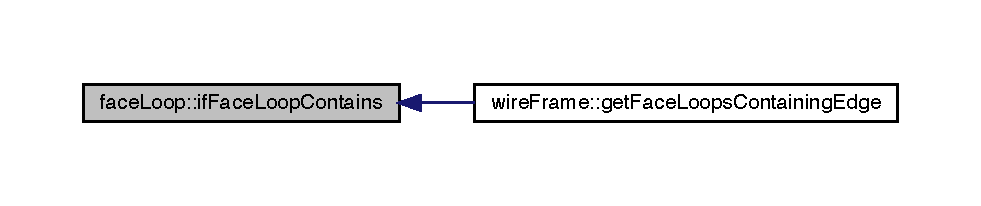
\includegraphics[width=350pt]{classface_loop_a3ed69fdb3554a255f484fa78fd1f3361_icgraph}
\end{center}
\end{figure}
\mbox{\Hypertarget{classface_loop_a603c5cfde9765657af9cf088df8fc474}\label{classface_loop_a603c5cfde9765657af9cf088df8fc474}} 
\index{face\+Loop@{face\+Loop}!operator==@{operator==}}
\index{operator==@{operator==}!face\+Loop@{face\+Loop}}
\subsubsection{\texorpdfstring{operator==()}{operator==()}}
{\footnotesize\ttfamily bool face\+Loop\+::operator== (\begin{DoxyParamCaption}\item[{\mbox{\hyperlink{classface_loop}{face\+Loop}}}]{other }\end{DoxyParamCaption}) const}

will arrange all the \mbox{\hyperlink{classbasic_loop_edge_set}{basic\+Loop\+Edge\+Set}} such that their direction is same as that of normal 

Definition at line 69 of file face\+Loop.\+cpp.

Here is the call graph for this function\+:
\nopagebreak
\begin{figure}[H]
\begin{center}
\leavevmode
\includegraphics[width=350pt]{classface_loop_a603c5cfde9765657af9cf088df8fc474_cgraph}
\end{center}
\end{figure}
\mbox{\Hypertarget{classface_loop_ac1c63792b00865fc45ad8934b5580e62}\label{classface_loop_ac1c63792b00865fc45ad8934b5580e62}} 
\index{face\+Loop@{face\+Loop}!remove\+Loop@{remove\+Loop}}
\index{remove\+Loop@{remove\+Loop}!face\+Loop@{face\+Loop}}
\subsubsection{\texorpdfstring{remove\+Loop()}{removeLoop()}}
{\footnotesize\ttfamily void face\+Loop\+::remove\+Loop (\begin{DoxyParamCaption}\item[{\mbox{\hyperlink{classbasic_loop_edge_set}{basic\+Loop\+Edge\+Set}}}]{loop }\end{DoxyParamCaption})}



Definition at line 16 of file face\+Loop.\+cpp.



\subsection{Member Data Documentation}
\mbox{\Hypertarget{classface_loop_a3f032bc5496c429abc4723632d29ceaf}\label{classface_loop_a3f032bc5496c429abc4723632d29ceaf}} 
\index{face\+Loop@{face\+Loop}!faceloop@{faceloop}}
\index{faceloop@{faceloop}!face\+Loop@{face\+Loop}}
\subsubsection{\texorpdfstring{faceloop}{faceloop}}
{\footnotesize\ttfamily vector$<$\mbox{\hyperlink{classbasic_loop_edge_set}{basic\+Loop\+Edge\+Set}}$>$ face\+Loop\+::faceloop}



Definition at line 20 of file face\+Loop.\+h.

\mbox{\Hypertarget{classface_loop_a2ac7efac9235e5d6c6c4694f2ea8a6c2}\label{classface_loop_a2ac7efac9235e5d6c6c4694f2ea8a6c2}} 
\index{face\+Loop@{face\+Loop}!normal@{normal}}
\index{normal@{normal}!face\+Loop@{face\+Loop}}
\subsubsection{\texorpdfstring{normal}{normal}}
{\footnotesize\ttfamily \mbox{\hyperlink{structdirection}{direction}} face\+Loop\+::normal}



Definition at line 21 of file face\+Loop.\+h.

\mbox{\Hypertarget{classface_loop_ace3e113db57081ef98d333a5bfd32daa}\label{classface_loop_ace3e113db57081ef98d333a5bfd32daa}} 
\index{face\+Loop@{face\+Loop}!p@{p}}
\index{p@{p}!face\+Loop@{face\+Loop}}
\subsubsection{\texorpdfstring{p}{p}}
{\footnotesize\ttfamily \mbox{\hyperlink{structplane}{plane}} face\+Loop\+::p}



Definition at line 22 of file face\+Loop.\+h.



The documentation for this class was generated from the following files\+:\begin{DoxyCompactItemize}
\item 
include/\mbox{\hyperlink{face_loop_8h}{face\+Loop.\+h}}\item 
src/\mbox{\hyperlink{face_loop_8cpp}{face\+Loop.\+cpp}}\end{DoxyCompactItemize}

\hypertarget{class_main_window}{}\section{Main\+Window Class Reference}
\label{class_main_window}\index{Main\+Window@{Main\+Window}}


{\ttfamily \#include $<$mainwindow.\+h$>$}



Inheritance diagram for Main\+Window\+:
\nopagebreak
\begin{figure}[H]
\begin{center}
\leavevmode
\includegraphics[width=161pt]{class_main_window__inherit__graph}
\end{center}
\end{figure}


Collaboration diagram for Main\+Window\+:
\nopagebreak
\begin{figure}[H]
\begin{center}
\leavevmode
\includegraphics[width=161pt]{class_main_window__coll__graph}
\end{center}
\end{figure}
\subsection*{Public Member Functions}
\begin{DoxyCompactItemize}
\item 
\mbox{\hyperlink{class_main_window_a8b244be8b7b7db1b08de2a2acb9409db}{Main\+Window}} (Q\+Widget $\ast$parent=0)
\item 
\mbox{\hyperlink{class_main_window_ae98d00a93bc118200eeef9f9bba1dba7}{$\sim$\+Main\+Window}} ()
\end{DoxyCompactItemize}


\subsection{Detailed Description}


Definition at line 10 of file mainwindow.\+h.



\subsection{Constructor \& Destructor Documentation}
\mbox{\Hypertarget{class_main_window_a8b244be8b7b7db1b08de2a2acb9409db}\label{class_main_window_a8b244be8b7b7db1b08de2a2acb9409db}} 
\index{Main\+Window@{Main\+Window}!Main\+Window@{Main\+Window}}
\index{Main\+Window@{Main\+Window}!Main\+Window@{Main\+Window}}
\subsubsection{\texorpdfstring{Main\+Window()}{MainWindow()}}
{\footnotesize\ttfamily Main\+Window\+::\+Main\+Window (\begin{DoxyParamCaption}\item[{Q\+Widget $\ast$}]{parent = {\ttfamily 0} }\end{DoxyParamCaption})\hspace{0.3cm}{\ttfamily [explicit]}}



Definition at line 5 of file mainwindow.\+cpp.

Here is the call graph for this function\+:
\nopagebreak
\begin{figure}[H]
\begin{center}
\leavevmode
\includegraphics[width=350pt]{class_main_window_a8b244be8b7b7db1b08de2a2acb9409db_cgraph}
\end{center}
\end{figure}
\mbox{\Hypertarget{class_main_window_ae98d00a93bc118200eeef9f9bba1dba7}\label{class_main_window_ae98d00a93bc118200eeef9f9bba1dba7}} 
\index{Main\+Window@{Main\+Window}!````~Main\+Window@{$\sim$\+Main\+Window}}
\index{````~Main\+Window@{$\sim$\+Main\+Window}!Main\+Window@{Main\+Window}}
\subsubsection{\texorpdfstring{$\sim$\+Main\+Window()}{~MainWindow()}}
{\footnotesize\ttfamily Main\+Window\+::$\sim$\+Main\+Window (\begin{DoxyParamCaption}{ }\end{DoxyParamCaption})}



Definition at line 12 of file mainwindow.\+cpp.



The documentation for this class was generated from the following files\+:\begin{DoxyCompactItemize}
\item 
include/\mbox{\hyperlink{mainwindow_8h}{mainwindow.\+h}}\item 
src/\mbox{\hyperlink{mainwindow_8cpp}{mainwindow.\+cpp}}\end{DoxyCompactItemize}

\hypertarget{class_ui_1_1_main_window}{}\section{Ui\+:\+:Main\+Window Class Reference}
\label{class_ui_1_1_main_window}\index{Ui\+::\+Main\+Window@{Ui\+::\+Main\+Window}}


{\ttfamily \#include $<$ui\+\_\+mainwindow.\+h$>$}



Inheritance diagram for Ui\+:\+:Main\+Window\+:
\nopagebreak
\begin{figure}[H]
\begin{center}
\leavevmode
\includegraphics[width=168pt]{class_ui_1_1_main_window__inherit__graph}
\end{center}
\end{figure}


Collaboration diagram for Ui\+:\+:Main\+Window\+:
\nopagebreak
\begin{figure}[H]
\begin{center}
\leavevmode
\includegraphics[width=168pt]{class_ui_1_1_main_window__coll__graph}
\end{center}
\end{figure}
\subsection*{Additional Inherited Members}


\subsection{Detailed Description}


Definition at line 137 of file ui\+\_\+mainwindow.\+h.



The documentation for this class was generated from the following file\+:\begin{DoxyCompactItemize}
\item 
include/\mbox{\hyperlink{ui__mainwindow_8h}{ui\+\_\+mainwindow.\+h}}\end{DoxyCompactItemize}

\hypertarget{class_options}{}\section{Options Class Reference}
\label{class_options}\index{Options@{Options}}


{\ttfamily \#include $<$options.\+h$>$}



Inheritance diagram for Options\+:
\nopagebreak
\begin{figure}[H]
\begin{center}
\leavevmode
\includegraphics[width=135pt]{class_options__inherit__graph}
\end{center}
\end{figure}


Collaboration diagram for Options\+:
\nopagebreak
\begin{figure}[H]
\begin{center}
\leavevmode
\includegraphics[width=135pt]{class_options__coll__graph}
\end{center}
\end{figure}
\subsection*{Public Member Functions}
\begin{DoxyCompactItemize}
\item 
\mbox{\hyperlink{class_options_a87403ad1d6bd9ae2b54af860bb0f0952}{Options}} (Q\+Widget $\ast$parent=0)
\end{DoxyCompactItemize}


\subsection{Detailed Description}


Definition at line 6 of file options.\+h.



\subsection{Constructor \& Destructor Documentation}
\mbox{\Hypertarget{class_options_a87403ad1d6bd9ae2b54af860bb0f0952}\label{class_options_a87403ad1d6bd9ae2b54af860bb0f0952}} 
\index{Options@{Options}!Options@{Options}}
\index{Options@{Options}!Options@{Options}}
\subsubsection{\texorpdfstring{Options()}{Options()}}
{\footnotesize\ttfamily Options\+::\+Options (\begin{DoxyParamCaption}\item[{Q\+Widget $\ast$}]{parent = {\ttfamily 0} }\end{DoxyParamCaption})\hspace{0.3cm}{\ttfamily [explicit]}}



Definition at line 3 of file options.\+cpp.



The documentation for this class was generated from the following files\+:\begin{DoxyCompactItemize}
\item 
include/\mbox{\hyperlink{options_8h}{options.\+h}}\item 
src/\mbox{\hyperlink{options_8cpp}{options.\+cpp}}\end{DoxyCompactItemize}

\hypertarget{structplane}{}\section{plane Struct Reference}
\label{structplane}\index{plane@{plane}}


{\ttfamily \#include $<$structs.\+h$>$}

\subsection*{Public Member Functions}
\begin{DoxyCompactItemize}
\item 
bool \mbox{\hyperlink{structplane_a7362172307c64ca0ba40633337f318ca}{operator==}} (const \mbox{\hyperlink{structplane}{plane}} \&rhs)
\end{DoxyCompactItemize}
\subsection*{Public Attributes}
\begin{DoxyCompactItemize}
\item 
float \mbox{\hyperlink{structplane_a93c319b577955eca012b2866db926c1f}{a}}
\item 
float \mbox{\hyperlink{structplane_af4a97d4328067448317dd787e048bc70}{b}}
\item 
float \mbox{\hyperlink{structplane_a3024e149a5b2cb4697fa71ae7d539bd1}{c}}
\item 
float \mbox{\hyperlink{structplane_a9a3cb65698785bad8199e7afbd083e27}{d}}
\end{DoxyCompactItemize}


\subsection{Detailed Description}


Definition at line 186 of file structs.\+h.



\subsection{Member Function Documentation}
\mbox{\Hypertarget{structplane_a7362172307c64ca0ba40633337f318ca}\label{structplane_a7362172307c64ca0ba40633337f318ca}} 
\index{plane@{plane}!operator==@{operator==}}
\index{operator==@{operator==}!plane@{plane}}
\subsubsection{\texorpdfstring{operator==()}{operator==()}}
{\footnotesize\ttfamily bool plane\+::operator== (\begin{DoxyParamCaption}\item[{const \mbox{\hyperlink{structplane}{plane}} \&}]{rhs }\end{DoxyParamCaption})\hspace{0.3cm}{\ttfamily [inline]}}



Definition at line 194 of file structs.\+h.

Here is the call graph for this function\+:
\nopagebreak
\begin{figure}[H]
\begin{center}
\leavevmode
\includegraphics[width=285pt]{structplane_a7362172307c64ca0ba40633337f318ca_cgraph}
\end{center}
\end{figure}


\subsection{Member Data Documentation}
\mbox{\Hypertarget{structplane_a93c319b577955eca012b2866db926c1f}\label{structplane_a93c319b577955eca012b2866db926c1f}} 
\index{plane@{plane}!a@{a}}
\index{a@{a}!plane@{plane}}
\subsubsection{\texorpdfstring{a}{a}}
{\footnotesize\ttfamily float plane\+::a}



Definition at line 188 of file structs.\+h.

\mbox{\Hypertarget{structplane_af4a97d4328067448317dd787e048bc70}\label{structplane_af4a97d4328067448317dd787e048bc70}} 
\index{plane@{plane}!b@{b}}
\index{b@{b}!plane@{plane}}
\subsubsection{\texorpdfstring{b}{b}}
{\footnotesize\ttfamily float plane\+::b}



Definition at line 189 of file structs.\+h.

\mbox{\Hypertarget{structplane_a3024e149a5b2cb4697fa71ae7d539bd1}\label{structplane_a3024e149a5b2cb4697fa71ae7d539bd1}} 
\index{plane@{plane}!c@{c}}
\index{c@{c}!plane@{plane}}
\subsubsection{\texorpdfstring{c}{c}}
{\footnotesize\ttfamily float plane\+::c}



Definition at line 190 of file structs.\+h.

\mbox{\Hypertarget{structplane_a9a3cb65698785bad8199e7afbd083e27}\label{structplane_a9a3cb65698785bad8199e7afbd083e27}} 
\index{plane@{plane}!d@{d}}
\index{d@{d}!plane@{plane}}
\subsubsection{\texorpdfstring{d}{d}}
{\footnotesize\ttfamily float plane\+::d}



Definition at line 191 of file structs.\+h.



The documentation for this struct was generated from the following file\+:\begin{DoxyCompactItemize}
\item 
include/\mbox{\hyperlink{structs_8h}{structs.\+h}}\end{DoxyCompactItemize}

\hypertarget{class_plane}{}\section{Plane Class Reference}
\label{class_plane}\index{Plane@{Plane}}


{\ttfamily \#include $<$Plane.\+h$>$}



Collaboration diagram for Plane\+:
\nopagebreak
\begin{figure}[H]
\begin{center}
\leavevmode
\includegraphics[width=122pt]{class_plane__coll__graph}
\end{center}
\end{figure}
\subsection*{Public Member Functions}
\begin{DoxyCompactItemize}
\item 
void \mbox{\hyperlink{class_plane_ad2708bd985955c7f978a191f4e9249ac}{sort\+Edges\+On\+Vertices}} ()
\end{DoxyCompactItemize}
\subsection*{Public Attributes}
\begin{DoxyCompactItemize}
\item 
\mbox{\hyperlink{structplane}{plane}} \mbox{\hyperlink{class_plane_a65c157cab5de9f5c3c1ecd5b7770badc}{p}}
\begin{DoxyCompactList}\small\item\em struct plane that defines a plane \end{DoxyCompactList}\item 
std\+::vector$<$ \mbox{\hyperlink{structvertex3_d}{vertex3D}} $>$ \mbox{\hyperlink{class_plane_a9badd6fb24525ce9605a3f6a5bb0d770}{v\+List}}
\begin{DoxyCompactList}\small\item\em list of all vertices on the plane \end{DoxyCompactList}\item 
std\+::vector$<$ \mbox{\hyperlink{structedge3_d}{edge3D}} $>$ \mbox{\hyperlink{class_plane_a71c027d1ed3593af105dcbdee9e1b11f}{e\+List}}
\begin{DoxyCompactList}\small\item\em list of all edges on the plane \end{DoxyCompactList}\item 
std\+::vector$<$ \mbox{\hyperlink{structvertex_edge_list}{vertex\+Edge\+List}} $>$ \mbox{\hyperlink{class_plane_a83494ec7ac0ca05a7fb8e8340c3a99fc}{ve\+List\+List}}
\begin{DoxyCompactList}\small\item\em list of vetex-\/edges\+On\+Vertex for all vertices on the plane \end{DoxyCompactList}\end{DoxyCompactItemize}


\subsection{Detailed Description}


Definition at line 11 of file Plane.\+h.



\subsection{Member Function Documentation}
\mbox{\Hypertarget{class_plane_ad2708bd985955c7f978a191f4e9249ac}\label{class_plane_ad2708bd985955c7f978a191f4e9249ac}} 
\index{Plane@{Plane}!sort\+Edges\+On\+Vertices@{sort\+Edges\+On\+Vertices}}
\index{sort\+Edges\+On\+Vertices@{sort\+Edges\+On\+Vertices}!Plane@{Plane}}
\subsubsection{\texorpdfstring{sort\+Edges\+On\+Vertices()}{sortEdgesOnVertices()}}
{\footnotesize\ttfamily void Plane\+::sort\+Edges\+On\+Vertices (\begin{DoxyParamCaption}{ }\end{DoxyParamCaption})}

applies the method sort\+Edges\+On\+Vertex on each vertex of a plane just modifies the \char`\"{}std\+::vector$<$vertex\+Edge\+List$>$ ve\+List\char`\"{} with edges sorted on each vertex 

Definition at line 68 of file Plane.\+cpp.



\subsection{Member Data Documentation}
\mbox{\Hypertarget{class_plane_a71c027d1ed3593af105dcbdee9e1b11f}\label{class_plane_a71c027d1ed3593af105dcbdee9e1b11f}} 
\index{Plane@{Plane}!e\+List@{e\+List}}
\index{e\+List@{e\+List}!Plane@{Plane}}
\subsubsection{\texorpdfstring{e\+List}{eList}}
{\footnotesize\ttfamily std\+::vector$<$\mbox{\hyperlink{structedge3_d}{edge3D}}$>$ Plane\+::e\+List}



list of all edges on the plane 



Definition at line 21 of file Plane.\+h.

\mbox{\Hypertarget{class_plane_a65c157cab5de9f5c3c1ecd5b7770badc}\label{class_plane_a65c157cab5de9f5c3c1ecd5b7770badc}} 
\index{Plane@{Plane}!p@{p}}
\index{p@{p}!Plane@{Plane}}
\subsubsection{\texorpdfstring{p}{p}}
{\footnotesize\ttfamily \mbox{\hyperlink{structplane}{plane}} Plane\+::p}



struct plane that defines a plane 



Definition at line 15 of file Plane.\+h.

\mbox{\Hypertarget{class_plane_a83494ec7ac0ca05a7fb8e8340c3a99fc}\label{class_plane_a83494ec7ac0ca05a7fb8e8340c3a99fc}} 
\index{Plane@{Plane}!ve\+List\+List@{ve\+List\+List}}
\index{ve\+List\+List@{ve\+List\+List}!Plane@{Plane}}
\subsubsection{\texorpdfstring{ve\+List\+List}{veListList}}
{\footnotesize\ttfamily std\+::vector$<$\mbox{\hyperlink{structvertex_edge_list}{vertex\+Edge\+List}}$>$ Plane\+::ve\+List\+List}



list of vetex-\/edges\+On\+Vertex for all vertices on the plane 



Definition at line 24 of file Plane.\+h.

\mbox{\Hypertarget{class_plane_a9badd6fb24525ce9605a3f6a5bb0d770}\label{class_plane_a9badd6fb24525ce9605a3f6a5bb0d770}} 
\index{Plane@{Plane}!v\+List@{v\+List}}
\index{v\+List@{v\+List}!Plane@{Plane}}
\subsubsection{\texorpdfstring{v\+List}{vList}}
{\footnotesize\ttfamily std\+::vector$<$\mbox{\hyperlink{structvertex3_d}{vertex3D}}$>$ Plane\+::v\+List}



list of all vertices on the plane 



Definition at line 18 of file Plane.\+h.



The documentation for this class was generated from the following files\+:\begin{DoxyCompactItemize}
\item 
include/\mbox{\hyperlink{_plane_8h}{Plane.\+h}}\item 
src/\mbox{\hyperlink{_plane_8cpp}{Plane.\+cpp}}\end{DoxyCompactItemize}

\hypertarget{structplane_v_e_l}{}\section{plane\+V\+EL Struct Reference}
\label{structplane_v_e_l}\index{plane\+V\+EL@{plane\+V\+EL}}


{\ttfamily \#include $<$structs.\+h$>$}



Collaboration diagram for plane\+V\+EL\+:
\nopagebreak
\begin{figure}[H]
\begin{center}
\leavevmode
\includegraphics[width=139pt]{structplane_v_e_l__coll__graph}
\end{center}
\end{figure}
\subsection*{Public Member Functions}
\begin{DoxyCompactItemize}
\item 
\mbox{\hyperlink{structplane_v_e_l_a23bf21cc557fa38db7a07cf77a22973d}{plane\+V\+EL}} ()
\item 
\mbox{\hyperlink{structplane_v_e_l_a6213d9d6eb1591469b48157ee1c0110b}{plane\+V\+EL}} (\mbox{\hyperlink{structplane}{plane}} pl, std\+::vector$<$ \mbox{\hyperlink{structvertex_edge_list}{vertex\+Edge\+List}} $>$ v)
\end{DoxyCompactItemize}
\subsection*{Public Attributes}
\begin{DoxyCompactItemize}
\item 
\mbox{\hyperlink{structplane}{plane}} \mbox{\hyperlink{structplane_v_e_l_a8ea259111525aaae0eb47c16ee2b1294}{p}}
\item 
std\+::vector$<$ \mbox{\hyperlink{structvertex_edge_list}{vertex\+Edge\+List}} $>$ \mbox{\hyperlink{structplane_v_e_l_af46afbe3061e68d08132aec85b94deb8}{vel\+List}}
\end{DoxyCompactItemize}


\subsection{Detailed Description}


Definition at line 262 of file structs.\+h.



\subsection{Constructor \& Destructor Documentation}
\mbox{\Hypertarget{structplane_v_e_l_a23bf21cc557fa38db7a07cf77a22973d}\label{structplane_v_e_l_a23bf21cc557fa38db7a07cf77a22973d}} 
\index{plane\+V\+EL@{plane\+V\+EL}!plane\+V\+EL@{plane\+V\+EL}}
\index{plane\+V\+EL@{plane\+V\+EL}!plane\+V\+EL@{plane\+V\+EL}}
\subsubsection{\texorpdfstring{plane\+V\+E\+L()}{planeVEL()}\hspace{0.1cm}{\footnotesize\ttfamily [1/2]}}
{\footnotesize\ttfamily plane\+V\+E\+L\+::plane\+V\+EL (\begin{DoxyParamCaption}{ }\end{DoxyParamCaption})\hspace{0.3cm}{\ttfamily [inline]}}



Definition at line 267 of file structs.\+h.

\mbox{\Hypertarget{structplane_v_e_l_a6213d9d6eb1591469b48157ee1c0110b}\label{structplane_v_e_l_a6213d9d6eb1591469b48157ee1c0110b}} 
\index{plane\+V\+EL@{plane\+V\+EL}!plane\+V\+EL@{plane\+V\+EL}}
\index{plane\+V\+EL@{plane\+V\+EL}!plane\+V\+EL@{plane\+V\+EL}}
\subsubsection{\texorpdfstring{plane\+V\+E\+L()}{planeVEL()}\hspace{0.1cm}{\footnotesize\ttfamily [2/2]}}
{\footnotesize\ttfamily plane\+V\+E\+L\+::plane\+V\+EL (\begin{DoxyParamCaption}\item[{\mbox{\hyperlink{structplane}{plane}}}]{pl,  }\item[{std\+::vector$<$ \mbox{\hyperlink{structvertex_edge_list}{vertex\+Edge\+List}} $>$}]{v }\end{DoxyParamCaption})\hspace{0.3cm}{\ttfamily [inline]}}



Definition at line 268 of file structs.\+h.



\subsection{Member Data Documentation}
\mbox{\Hypertarget{structplane_v_e_l_a8ea259111525aaae0eb47c16ee2b1294}\label{structplane_v_e_l_a8ea259111525aaae0eb47c16ee2b1294}} 
\index{plane\+V\+EL@{plane\+V\+EL}!p@{p}}
\index{p@{p}!plane\+V\+EL@{plane\+V\+EL}}
\subsubsection{\texorpdfstring{p}{p}}
{\footnotesize\ttfamily \mbox{\hyperlink{structplane}{plane}} plane\+V\+E\+L\+::p}



Definition at line 263 of file structs.\+h.

\mbox{\Hypertarget{structplane_v_e_l_af46afbe3061e68d08132aec85b94deb8}\label{structplane_v_e_l_af46afbe3061e68d08132aec85b94deb8}} 
\index{plane\+V\+EL@{plane\+V\+EL}!vel\+List@{vel\+List}}
\index{vel\+List@{vel\+List}!plane\+V\+EL@{plane\+V\+EL}}
\subsubsection{\texorpdfstring{vel\+List}{velList}}
{\footnotesize\ttfamily std\+::vector$<$\mbox{\hyperlink{structvertex_edge_list}{vertex\+Edge\+List}}$>$ plane\+V\+E\+L\+::vel\+List}



Definition at line 264 of file structs.\+h.



The documentation for this struct was generated from the following file\+:\begin{DoxyCompactItemize}
\item 
include/\mbox{\hyperlink{structs_8h}{structs.\+h}}\end{DoxyCompactItemize}

\hypertarget{structqt__meta__stringdata___main_window__t}{}\section{qt\+\_\+meta\+\_\+stringdata\+\_\+\+Main\+Window\+\_\+t Struct Reference}
\label{structqt__meta__stringdata___main_window__t}\index{qt\+\_\+meta\+\_\+stringdata\+\_\+\+Main\+Window\+\_\+t@{qt\+\_\+meta\+\_\+stringdata\+\_\+\+Main\+Window\+\_\+t}}
\subsection*{Public Attributes}
\begin{DoxyCompactItemize}
\item 
Q\+Byte\+Array\+Data \mbox{\hyperlink{structqt__meta__stringdata___main_window__t_a092956d0ba2e51cd73092e8a5ebb6ce6}{data}} \mbox{[}8\mbox{]}
\item 
char \mbox{\hyperlink{structqt__meta__stringdata___main_window__t_a17b51b6af12b7f5ebb4f7b55545039db}{stringdata0}} \mbox{[}145\mbox{]}
\end{DoxyCompactItemize}


\subsection{Detailed Description}


Definition at line 21 of file moc\+\_\+mainwindow.\+cpp.



\subsection{Member Data Documentation}
\mbox{\Hypertarget{structqt__meta__stringdata___main_window__t_a092956d0ba2e51cd73092e8a5ebb6ce6}\label{structqt__meta__stringdata___main_window__t_a092956d0ba2e51cd73092e8a5ebb6ce6}} 
\index{qt\+\_\+meta\+\_\+stringdata\+\_\+\+Main\+Window\+\_\+t@{qt\+\_\+meta\+\_\+stringdata\+\_\+\+Main\+Window\+\_\+t}!data@{data}}
\index{data@{data}!qt\+\_\+meta\+\_\+stringdata\+\_\+\+Main\+Window\+\_\+t@{qt\+\_\+meta\+\_\+stringdata\+\_\+\+Main\+Window\+\_\+t}}
\subsubsection{\texorpdfstring{data}{data}}
{\footnotesize\ttfamily Q\+Byte\+Array\+Data qt\+\_\+meta\+\_\+stringdata\+\_\+\+Main\+Window\+\_\+t\+::data}



Definition at line 22 of file moc\+\_\+mainwindow.\+cpp.

\mbox{\Hypertarget{structqt__meta__stringdata___main_window__t_a17b51b6af12b7f5ebb4f7b55545039db}\label{structqt__meta__stringdata___main_window__t_a17b51b6af12b7f5ebb4f7b55545039db}} 
\index{qt\+\_\+meta\+\_\+stringdata\+\_\+\+Main\+Window\+\_\+t@{qt\+\_\+meta\+\_\+stringdata\+\_\+\+Main\+Window\+\_\+t}!stringdata0@{stringdata0}}
\index{stringdata0@{stringdata0}!qt\+\_\+meta\+\_\+stringdata\+\_\+\+Main\+Window\+\_\+t@{qt\+\_\+meta\+\_\+stringdata\+\_\+\+Main\+Window\+\_\+t}}
\subsubsection{\texorpdfstring{stringdata0}{stringdata0}}
{\footnotesize\ttfamily char qt\+\_\+meta\+\_\+stringdata\+\_\+\+Main\+Window\+\_\+t\+::stringdata0}



Definition at line 23 of file moc\+\_\+mainwindow.\+cpp.



The documentation for this struct was generated from the following file\+:\begin{DoxyCompactItemize}
\item 
build/\mbox{\hyperlink{build_2moc__mainwindow_8cpp}{moc\+\_\+mainwindow.\+cpp}}\end{DoxyCompactItemize}

\hypertarget{structqt__meta__stringdata___options__t}{}\section{qt\+\_\+meta\+\_\+stringdata\+\_\+\+Options\+\_\+t Struct Reference}
\label{structqt__meta__stringdata___options__t}\index{qt\+\_\+meta\+\_\+stringdata\+\_\+\+Options\+\_\+t@{qt\+\_\+meta\+\_\+stringdata\+\_\+\+Options\+\_\+t}}
\subsection*{Public Attributes}
\begin{DoxyCompactItemize}
\item 
Q\+Byte\+Array\+Data \mbox{\hyperlink{structqt__meta__stringdata___options__t_ad630fb0469c0871580fa3053b9b09bb8}{data}} \mbox{[}1\mbox{]}
\item 
char \mbox{\hyperlink{structqt__meta__stringdata___options__t_a1c10b521fc0bfc89e2ad3c4ae2bc0b34}{stringdata0}} \mbox{[}8\mbox{]}
\end{DoxyCompactItemize}


\subsection{Detailed Description}


Definition at line 21 of file moc\+\_\+options.\+cpp.



\subsection{Member Data Documentation}
\mbox{\Hypertarget{structqt__meta__stringdata___options__t_ad630fb0469c0871580fa3053b9b09bb8}\label{structqt__meta__stringdata___options__t_ad630fb0469c0871580fa3053b9b09bb8}} 
\index{qt\+\_\+meta\+\_\+stringdata\+\_\+\+Options\+\_\+t@{qt\+\_\+meta\+\_\+stringdata\+\_\+\+Options\+\_\+t}!data@{data}}
\index{data@{data}!qt\+\_\+meta\+\_\+stringdata\+\_\+\+Options\+\_\+t@{qt\+\_\+meta\+\_\+stringdata\+\_\+\+Options\+\_\+t}}
\subsubsection{\texorpdfstring{data}{data}}
{\footnotesize\ttfamily Q\+Byte\+Array\+Data qt\+\_\+meta\+\_\+stringdata\+\_\+\+Options\+\_\+t\+::data}



Definition at line 22 of file moc\+\_\+options.\+cpp.

\mbox{\Hypertarget{structqt__meta__stringdata___options__t_a1c10b521fc0bfc89e2ad3c4ae2bc0b34}\label{structqt__meta__stringdata___options__t_a1c10b521fc0bfc89e2ad3c4ae2bc0b34}} 
\index{qt\+\_\+meta\+\_\+stringdata\+\_\+\+Options\+\_\+t@{qt\+\_\+meta\+\_\+stringdata\+\_\+\+Options\+\_\+t}!stringdata0@{stringdata0}}
\index{stringdata0@{stringdata0}!qt\+\_\+meta\+\_\+stringdata\+\_\+\+Options\+\_\+t@{qt\+\_\+meta\+\_\+stringdata\+\_\+\+Options\+\_\+t}}
\subsubsection{\texorpdfstring{stringdata0}{stringdata0}}
{\footnotesize\ttfamily char qt\+\_\+meta\+\_\+stringdata\+\_\+\+Options\+\_\+t\+::stringdata0}



Definition at line 23 of file moc\+\_\+options.\+cpp.



The documentation for this struct was generated from the following file\+:\begin{DoxyCompactItemize}
\item 
build/\mbox{\hyperlink{build_2moc__options_8cpp}{moc\+\_\+options.\+cpp}}\end{DoxyCompactItemize}

\hypertarget{structqt__meta__stringdata___selection__t}{}\section{qt\+\_\+meta\+\_\+stringdata\+\_\+\+Selection\+\_\+t Struct Reference}
\label{structqt__meta__stringdata___selection__t}\index{qt\+\_\+meta\+\_\+stringdata\+\_\+\+Selection\+\_\+t@{qt\+\_\+meta\+\_\+stringdata\+\_\+\+Selection\+\_\+t}}
\subsection*{Public Attributes}
\begin{DoxyCompactItemize}
\item 
Q\+Byte\+Array\+Data \mbox{\hyperlink{structqt__meta__stringdata___selection__t_ac153f153e95caf143389140d4e56cd5b}{data}} \mbox{[}4\mbox{]}
\item 
char \mbox{\hyperlink{structqt__meta__stringdata___selection__t_aebaf48c958bfda11e969b41fc7e0a2eb}{stringdata0}} \mbox{[}52\mbox{]}
\end{DoxyCompactItemize}


\subsection{Detailed Description}


Definition at line 21 of file moc\+\_\+selection.\+cpp.



\subsection{Member Data Documentation}
\mbox{\Hypertarget{structqt__meta__stringdata___selection__t_ac153f153e95caf143389140d4e56cd5b}\label{structqt__meta__stringdata___selection__t_ac153f153e95caf143389140d4e56cd5b}} 
\index{qt\+\_\+meta\+\_\+stringdata\+\_\+\+Selection\+\_\+t@{qt\+\_\+meta\+\_\+stringdata\+\_\+\+Selection\+\_\+t}!data@{data}}
\index{data@{data}!qt\+\_\+meta\+\_\+stringdata\+\_\+\+Selection\+\_\+t@{qt\+\_\+meta\+\_\+stringdata\+\_\+\+Selection\+\_\+t}}
\subsubsection{\texorpdfstring{data}{data}}
{\footnotesize\ttfamily Q\+Byte\+Array\+Data qt\+\_\+meta\+\_\+stringdata\+\_\+\+Selection\+\_\+t\+::data}



Definition at line 22 of file moc\+\_\+selection.\+cpp.

\mbox{\Hypertarget{structqt__meta__stringdata___selection__t_aebaf48c958bfda11e969b41fc7e0a2eb}\label{structqt__meta__stringdata___selection__t_aebaf48c958bfda11e969b41fc7e0a2eb}} 
\index{qt\+\_\+meta\+\_\+stringdata\+\_\+\+Selection\+\_\+t@{qt\+\_\+meta\+\_\+stringdata\+\_\+\+Selection\+\_\+t}!stringdata0@{stringdata0}}
\index{stringdata0@{stringdata0}!qt\+\_\+meta\+\_\+stringdata\+\_\+\+Selection\+\_\+t@{qt\+\_\+meta\+\_\+stringdata\+\_\+\+Selection\+\_\+t}}
\subsubsection{\texorpdfstring{stringdata0}{stringdata0}}
{\footnotesize\ttfamily char qt\+\_\+meta\+\_\+stringdata\+\_\+\+Selection\+\_\+t\+::stringdata0}



Definition at line 23 of file moc\+\_\+selection.\+cpp.



The documentation for this struct was generated from the following file\+:\begin{DoxyCompactItemize}
\item 
build/\mbox{\hyperlink{build_2moc__selection_8cpp}{moc\+\_\+selection.\+cpp}}\end{DoxyCompactItemize}

\hypertarget{structqt__meta__stringdata___show_projections__t}{}\section{qt\+\_\+meta\+\_\+stringdata\+\_\+\+Show\+Projections\+\_\+t Struct Reference}
\label{structqt__meta__stringdata___show_projections__t}\index{qt\+\_\+meta\+\_\+stringdata\+\_\+\+Show\+Projections\+\_\+t@{qt\+\_\+meta\+\_\+stringdata\+\_\+\+Show\+Projections\+\_\+t}}
\subsection*{Public Attributes}
\begin{DoxyCompactItemize}
\item 
Q\+Byte\+Array\+Data \mbox{\hyperlink{structqt__meta__stringdata___show_projections__t_ad29371ea2a69e8ca9aafddbe5c999c15}{data}} \mbox{[}8\mbox{]}
\item 
char \mbox{\hyperlink{structqt__meta__stringdata___show_projections__t_ac38af3ba9c6d74086b384b5d28cfa298}{stringdata0}} \mbox{[}150\mbox{]}
\end{DoxyCompactItemize}


\subsection{Detailed Description}


Definition at line 21 of file moc\+\_\+showprojections.\+cpp.



\subsection{Member Data Documentation}
\mbox{\Hypertarget{structqt__meta__stringdata___show_projections__t_ad29371ea2a69e8ca9aafddbe5c999c15}\label{structqt__meta__stringdata___show_projections__t_ad29371ea2a69e8ca9aafddbe5c999c15}} 
\index{qt\+\_\+meta\+\_\+stringdata\+\_\+\+Show\+Projections\+\_\+t@{qt\+\_\+meta\+\_\+stringdata\+\_\+\+Show\+Projections\+\_\+t}!data@{data}}
\index{data@{data}!qt\+\_\+meta\+\_\+stringdata\+\_\+\+Show\+Projections\+\_\+t@{qt\+\_\+meta\+\_\+stringdata\+\_\+\+Show\+Projections\+\_\+t}}
\subsubsection{\texorpdfstring{data}{data}}
{\footnotesize\ttfamily Q\+Byte\+Array\+Data qt\+\_\+meta\+\_\+stringdata\+\_\+\+Show\+Projections\+\_\+t\+::data\mbox{[}8\mbox{]}}



Definition at line 22 of file moc\+\_\+showprojections.\+cpp.

\mbox{\Hypertarget{structqt__meta__stringdata___show_projections__t_ac38af3ba9c6d74086b384b5d28cfa298}\label{structqt__meta__stringdata___show_projections__t_ac38af3ba9c6d74086b384b5d28cfa298}} 
\index{qt\+\_\+meta\+\_\+stringdata\+\_\+\+Show\+Projections\+\_\+t@{qt\+\_\+meta\+\_\+stringdata\+\_\+\+Show\+Projections\+\_\+t}!stringdata0@{stringdata0}}
\index{stringdata0@{stringdata0}!qt\+\_\+meta\+\_\+stringdata\+\_\+\+Show\+Projections\+\_\+t@{qt\+\_\+meta\+\_\+stringdata\+\_\+\+Show\+Projections\+\_\+t}}
\subsubsection{\texorpdfstring{stringdata0}{stringdata0}}
{\footnotesize\ttfamily char qt\+\_\+meta\+\_\+stringdata\+\_\+\+Show\+Projections\+\_\+t\+::stringdata0\mbox{[}150\mbox{]}}



Definition at line 23 of file moc\+\_\+showprojections.\+cpp.



The documentation for this struct was generated from the following file\+:\begin{DoxyCompactItemize}
\item 
src/\mbox{\hyperlink{moc__showprojections_8cpp}{moc\+\_\+showprojections.\+cpp}}\end{DoxyCompactItemize}

\hypertarget{class_selection}{}\section{Selection Class Reference}
\label{class_selection}\index{Selection@{Selection}}


{\ttfamily \#include $<$selection.\+h$>$}



Inheritance diagram for Selection\+:
\nopagebreak
\begin{figure}[H]
\begin{center}
\leavevmode
\includegraphics[width=161pt]{class_selection__inherit__graph}
\end{center}
\end{figure}


Collaboration diagram for Selection\+:
\nopagebreak
\begin{figure}[H]
\begin{center}
\leavevmode
\includegraphics[width=161pt]{class_selection__coll__graph}
\end{center}
\end{figure}
\subsection*{Public Member Functions}
\begin{DoxyCompactItemize}
\item 
\mbox{\hyperlink{class_selection_ab6a737100a92cf8dd040b6b7b439c5c1}{Selection}} (Q\+Widget $\ast$parent=0)
\item 
\mbox{\hyperlink{class_selection_a1860ec524d11c03de8c10a9354319839}{$\sim$\+Selection}} ()
\end{DoxyCompactItemize}


\subsection{Detailed Description}


Definition at line 10 of file selection.\+h.



\subsection{Constructor \& Destructor Documentation}
\mbox{\Hypertarget{class_selection_ab6a737100a92cf8dd040b6b7b439c5c1}\label{class_selection_ab6a737100a92cf8dd040b6b7b439c5c1}} 
\index{Selection@{Selection}!Selection@{Selection}}
\index{Selection@{Selection}!Selection@{Selection}}
\subsubsection{\texorpdfstring{Selection()}{Selection()}}
{\footnotesize\ttfamily Selection\+::\+Selection (\begin{DoxyParamCaption}\item[{Q\+Widget $\ast$}]{parent = {\ttfamily 0} }\end{DoxyParamCaption})\hspace{0.3cm}{\ttfamily [explicit]}}



Definition at line 36 of file selection.\+cpp.

Here is the call graph for this function\+:
\nopagebreak
\begin{figure}[H]
\begin{center}
\leavevmode
\includegraphics[width=350pt]{class_selection_ab6a737100a92cf8dd040b6b7b439c5c1_cgraph}
\end{center}
\end{figure}
\mbox{\Hypertarget{class_selection_a1860ec524d11c03de8c10a9354319839}\label{class_selection_a1860ec524d11c03de8c10a9354319839}} 
\index{Selection@{Selection}!````~Selection@{$\sim$\+Selection}}
\index{````~Selection@{$\sim$\+Selection}!Selection@{Selection}}
\subsubsection{\texorpdfstring{$\sim$\+Selection()}{~Selection()}}
{\footnotesize\ttfamily Selection\+::$\sim$\+Selection (\begin{DoxyParamCaption}{ }\end{DoxyParamCaption})}



Definition at line 45 of file selection.\+cpp.



The documentation for this class was generated from the following files\+:\begin{DoxyCompactItemize}
\item 
include/\mbox{\hyperlink{selection_8h}{selection.\+h}}\item 
src/\mbox{\hyperlink{selection_8cpp}{selection.\+cpp}}\end{DoxyCompactItemize}

\hypertarget{class_ui_1_1_selection}{}\section{Ui\+:\+:Selection Class Reference}
\label{class_ui_1_1_selection}\index{Ui\+::\+Selection@{Ui\+::\+Selection}}


{\ttfamily \#include $<$ui\+\_\+selection.\+h$>$}



Inheritance diagram for Ui\+:\+:Selection\+:
\nopagebreak
\begin{figure}[H]
\begin{center}
\leavevmode
\includegraphics[width=152pt]{class_ui_1_1_selection__inherit__graph}
\end{center}
\end{figure}


Collaboration diagram for Ui\+:\+:Selection\+:
\nopagebreak
\begin{figure}[H]
\begin{center}
\leavevmode
\includegraphics[width=152pt]{class_ui_1_1_selection__coll__graph}
\end{center}
\end{figure}
\subsection*{Additional Inherited Members}


\subsection{Detailed Description}


Definition at line 71 of file ui\+\_\+selection.\+h.



The documentation for this class was generated from the following file\+:\begin{DoxyCompactItemize}
\item 
include/\mbox{\hyperlink{ui__selection_8h}{ui\+\_\+selection.\+h}}\end{DoxyCompactItemize}

\hypertarget{class_show_projections}{}\section{Show\+Projections Class Reference}
\label{class_show_projections}\index{Show\+Projections@{Show\+Projections}}


{\ttfamily \#include $<$showprojections.\+h$>$}



Inheritance diagram for Show\+Projections\+:
\nopagebreak
\begin{figure}[H]
\begin{center}
\leavevmode
\includegraphics[width=170pt]{class_show_projections__inherit__graph}
\end{center}
\end{figure}


Collaboration diagram for Show\+Projections\+:
\nopagebreak
\begin{figure}[H]
\begin{center}
\leavevmode
\includegraphics[width=244pt]{class_show_projections__coll__graph}
\end{center}
\end{figure}
\subsection*{Public Member Functions}
\begin{DoxyCompactItemize}
\item 
\mbox{\hyperlink{class_show_projections_a9d5dd82bfa3dc9b28aa04e4d643cd38b}{Show\+Projections}} (Q\+Widget $\ast$parent=0)
\item 
\mbox{\hyperlink{class_show_projections_a63c65a092f0ea092e48de24798df8732}{$\sim$\+Show\+Projections}} ()
\item 
void \mbox{\hyperlink{class_show_projections_aafb940c0c1400571770261580285137c}{generate\+View}} ()
\item 
void \mbox{\hyperlink{class_show_projections_aaaf367e35dded9fbb5971b5e5a134373}{draw}} ()
\end{DoxyCompactItemize}
\subsection*{Public Attributes}
\begin{DoxyCompactItemize}
\item 
float \mbox{\hyperlink{class_show_projections_a87d1471d46ccad3a64ef5e4d3cc34933}{angleX}}
\item 
float \mbox{\hyperlink{class_show_projections_a161c729ded314da8f1920b8ee5651f83}{angleY}}
\item 
float \mbox{\hyperlink{class_show_projections_acecb344bb7e7cfe5610ebaa19d31c90b}{angleZ}}
\item 
std\+::string \mbox{\hyperlink{class_show_projections_abcc6c94ecf29145f8ae94f02df4d8f50}{objfile\+Name}}
\item 
\mbox{\hyperlink{class_two_d_obj}{Two\+D\+Obj}} $\ast$ \mbox{\hyperlink{class_show_projections_a2fcd6111dcc0b378a7908a4e0ea2cd96}{two\+D\+Obj\+Attr}}
\end{DoxyCompactItemize}


\subsection{Detailed Description}


Definition at line 11 of file showprojections.\+h.



\subsection{Constructor \& Destructor Documentation}
\mbox{\Hypertarget{class_show_projections_a9d5dd82bfa3dc9b28aa04e4d643cd38b}\label{class_show_projections_a9d5dd82bfa3dc9b28aa04e4d643cd38b}} 
\index{Show\+Projections@{Show\+Projections}!Show\+Projections@{Show\+Projections}}
\index{Show\+Projections@{Show\+Projections}!Show\+Projections@{Show\+Projections}}
\subsubsection{\texorpdfstring{Show\+Projections()}{ShowProjections()}}
{\footnotesize\ttfamily Show\+Projections\+::\+Show\+Projections (\begin{DoxyParamCaption}\item[{Q\+Widget $\ast$}]{parent = {\ttfamily 0} }\end{DoxyParamCaption})\hspace{0.3cm}{\ttfamily [explicit]}}



Definition at line 31 of file showprojections.\+cpp.

Here is the call graph for this function\+:
\nopagebreak
\begin{figure}[H]
\begin{center}
\leavevmode
\includegraphics[width=350pt]{class_show_projections_a9d5dd82bfa3dc9b28aa04e4d643cd38b_cgraph}
\end{center}
\end{figure}
\mbox{\Hypertarget{class_show_projections_a63c65a092f0ea092e48de24798df8732}\label{class_show_projections_a63c65a092f0ea092e48de24798df8732}} 
\index{Show\+Projections@{Show\+Projections}!````~Show\+Projections@{$\sim$\+Show\+Projections}}
\index{````~Show\+Projections@{$\sim$\+Show\+Projections}!Show\+Projections@{Show\+Projections}}
\subsubsection{\texorpdfstring{$\sim$\+Show\+Projections()}{~ShowProjections()}}
{\footnotesize\ttfamily Show\+Projections\+::$\sim$\+Show\+Projections (\begin{DoxyParamCaption}{ }\end{DoxyParamCaption})}



Definition at line 41 of file showprojections.\+cpp.



\subsection{Member Function Documentation}
\mbox{\Hypertarget{class_show_projections_aaaf367e35dded9fbb5971b5e5a134373}\label{class_show_projections_aaaf367e35dded9fbb5971b5e5a134373}} 
\index{Show\+Projections@{Show\+Projections}!draw@{draw}}
\index{draw@{draw}!Show\+Projections@{Show\+Projections}}
\subsubsection{\texorpdfstring{draw()}{draw()}}
{\footnotesize\ttfamily void Show\+Projections\+::draw (\begin{DoxyParamCaption}{ }\end{DoxyParamCaption})}



Definition at line 367 of file showprojections.\+cpp.

Here is the call graph for this function\+:
\nopagebreak
\begin{figure}[H]
\begin{center}
\leavevmode
\includegraphics[width=350pt]{class_show_projections_aaaf367e35dded9fbb5971b5e5a134373_cgraph}
\end{center}
\end{figure}
Here is the caller graph for this function\+:
\nopagebreak
\begin{figure}[H]
\begin{center}
\leavevmode
\includegraphics[width=350pt]{class_show_projections_aaaf367e35dded9fbb5971b5e5a134373_icgraph}
\end{center}
\end{figure}
\mbox{\Hypertarget{class_show_projections_aafb940c0c1400571770261580285137c}\label{class_show_projections_aafb940c0c1400571770261580285137c}} 
\index{Show\+Projections@{Show\+Projections}!generate\+View@{generate\+View}}
\index{generate\+View@{generate\+View}!Show\+Projections@{Show\+Projections}}
\subsubsection{\texorpdfstring{generate\+View()}{generateView()}}
{\footnotesize\ttfamily void Show\+Projections\+::generate\+View (\begin{DoxyParamCaption}{ }\end{DoxyParamCaption})}



Definition at line 46 of file showprojections.\+cpp.

Here is the call graph for this function\+:
\nopagebreak
\begin{figure}[H]
\begin{center}
\leavevmode
\includegraphics[width=350pt]{class_show_projections_aafb940c0c1400571770261580285137c_cgraph}
\end{center}
\end{figure}


\subsection{Member Data Documentation}
\mbox{\Hypertarget{class_show_projections_a87d1471d46ccad3a64ef5e4d3cc34933}\label{class_show_projections_a87d1471d46ccad3a64ef5e4d3cc34933}} 
\index{Show\+Projections@{Show\+Projections}!angleX@{angleX}}
\index{angleX@{angleX}!Show\+Projections@{Show\+Projections}}
\subsubsection{\texorpdfstring{angleX}{angleX}}
{\footnotesize\ttfamily float Show\+Projections\+::angleX}



Definition at line 18 of file showprojections.\+h.

\mbox{\Hypertarget{class_show_projections_a161c729ded314da8f1920b8ee5651f83}\label{class_show_projections_a161c729ded314da8f1920b8ee5651f83}} 
\index{Show\+Projections@{Show\+Projections}!angleY@{angleY}}
\index{angleY@{angleY}!Show\+Projections@{Show\+Projections}}
\subsubsection{\texorpdfstring{angleY}{angleY}}
{\footnotesize\ttfamily float Show\+Projections\+::angleY}



Definition at line 18 of file showprojections.\+h.

\mbox{\Hypertarget{class_show_projections_acecb344bb7e7cfe5610ebaa19d31c90b}\label{class_show_projections_acecb344bb7e7cfe5610ebaa19d31c90b}} 
\index{Show\+Projections@{Show\+Projections}!angleZ@{angleZ}}
\index{angleZ@{angleZ}!Show\+Projections@{Show\+Projections}}
\subsubsection{\texorpdfstring{angleZ}{angleZ}}
{\footnotesize\ttfamily float Show\+Projections\+::angleZ}



Definition at line 18 of file showprojections.\+h.

\mbox{\Hypertarget{class_show_projections_abcc6c94ecf29145f8ae94f02df4d8f50}\label{class_show_projections_abcc6c94ecf29145f8ae94f02df4d8f50}} 
\index{Show\+Projections@{Show\+Projections}!objfile\+Name@{objfile\+Name}}
\index{objfile\+Name@{objfile\+Name}!Show\+Projections@{Show\+Projections}}
\subsubsection{\texorpdfstring{objfile\+Name}{objfileName}}
{\footnotesize\ttfamily std\+::string Show\+Projections\+::objfile\+Name}



Definition at line 19 of file showprojections.\+h.

\mbox{\Hypertarget{class_show_projections_a2fcd6111dcc0b378a7908a4e0ea2cd96}\label{class_show_projections_a2fcd6111dcc0b378a7908a4e0ea2cd96}} 
\index{Show\+Projections@{Show\+Projections}!two\+D\+Obj\+Attr@{two\+D\+Obj\+Attr}}
\index{two\+D\+Obj\+Attr@{two\+D\+Obj\+Attr}!Show\+Projections@{Show\+Projections}}
\subsubsection{\texorpdfstring{two\+D\+Obj\+Attr}{twoDObjAttr}}
{\footnotesize\ttfamily \mbox{\hyperlink{class_two_d_obj}{Two\+D\+Obj}}$\ast$ Show\+Projections\+::two\+D\+Obj\+Attr}



Definition at line 22 of file showprojections.\+h.



The documentation for this class was generated from the following files\+:\begin{DoxyCompactItemize}
\item 
include/\mbox{\hyperlink{showprojections_8h}{showprojections.\+h}}\item 
src/\mbox{\hyperlink{showprojections_8cpp}{showprojections.\+cpp}}\end{DoxyCompactItemize}

\hypertarget{class_ui_1_1_show_projections}{}\section{Ui\+:\+:Show\+Projections Class Reference}
\label{class_ui_1_1_show_projections}\index{Ui\+::\+Show\+Projections@{Ui\+::\+Show\+Projections}}


{\ttfamily \#include $<$ui\+\_\+showprojections.\+h$>$}



Inheritance diagram for Ui\+:\+:Show\+Projections\+:
\nopagebreak
\begin{figure}[H]
\begin{center}
\leavevmode
\includegraphics[width=185pt]{class_ui_1_1_show_projections__inherit__graph}
\end{center}
\end{figure}


Collaboration diagram for Ui\+:\+:Show\+Projections\+:
\nopagebreak
\begin{figure}[H]
\begin{center}
\leavevmode
\includegraphics[width=185pt]{class_ui_1_1_show_projections__coll__graph}
\end{center}
\end{figure}
\subsection*{Additional Inherited Members}


\subsection{Detailed Description}


Definition at line 150 of file ui\+\_\+showprojections.\+h.



The documentation for this class was generated from the following file\+:\begin{DoxyCompactItemize}
\item 
include/\mbox{\hyperlink{ui__showprojections_8h}{ui\+\_\+showprojections.\+h}}\end{DoxyCompactItemize}

\hypertarget{class_two_d_obj}{}\section{Two\+D\+Obj Class Reference}
\label{class_two_d_obj}\index{Two\+D\+Obj@{Two\+D\+Obj}}


{\ttfamily \#include $<$Two\+D\+Obj.\+h$>$}

\subsection*{Public Member Functions}
\begin{DoxyCompactItemize}
\item 
\mbox{\hyperlink{class_two_d_obj_aa3c92bdec23c2c687b3e238934e24590}{Two\+D\+Obj}} (std\+::vector$<$ \mbox{\hyperlink{structvertex3_d}{vertex3D}} $>$ \mbox{\hyperlink{class_two_d_obj_ae1325111bfe55914cdcb399bc299442b}{vertices}}, std\+::vector$<$ \mbox{\hyperlink{structedge3_d}{edge3D}} $>$ \mbox{\hyperlink{class_two_d_obj_a48a318d3eac2dc2f2997aa4a4dc2450f}{edge\+List}}, std\+::vector$<$ std\+::vector$<$ \mbox{\hyperlink{structvertex3_d}{vertex3D}} $>$ $>$)
\item 
void \mbox{\hyperlink{class_two_d_obj_a3e4e17ffd7b54bf442bfce6387ed4c27}{generate\+Top\+View}} ()
\begin{DoxyCompactList}\small\item\em generates Top View \end{DoxyCompactList}\item 
void \mbox{\hyperlink{class_two_d_obj_a40fa2f831edda30806a28e30ae0b0feb}{generate\+Front\+View}} ()
\begin{DoxyCompactList}\small\item\em generates Top View \end{DoxyCompactList}\item 
void \mbox{\hyperlink{class_two_d_obj_a19b8f32d11ae455e15297aefa0028967}{generate\+Side\+View}} ()
\item 
std\+::vector$<$ std\+::vector$<$ \mbox{\hyperlink{structedge2_d}{edge2D}} $>$ $>$ \mbox{\hyperlink{class_two_d_obj_a0e7b5705ad697c100b39a1475b46475a}{get\+Views}} ()
\item 
float $\ast$ \mbox{\hyperlink{class_two_d_obj_ab6d468aec6681bef559fc2f222d7063a}{get\+Min\+XY}} ()
\item 
void \mbox{\hyperlink{class_two_d_obj_a6df93c379589948f30db2eacfa5d68bb}{generate\+Isometric}} ()
\item 
bool \mbox{\hyperlink{class_two_d_obj_ab0d27341367906fc4f4d9e5e8b4b8543}{hidden\+In\+View}} (\mbox{\hyperlink{structedge3_d}{edge3D}} edge, int \mbox{\hyperlink{structdirection}{direction}})
\item 
bool \mbox{\hyperlink{class_two_d_obj_acd188f5b49cd1d8c21fde2d8646294fe}{check\+Hides}} (\mbox{\hyperlink{structedge3_d}{edge3D}} edge, std\+::vector$<$ \mbox{\hyperlink{structvertex3_d}{vertex3D}} $>$ plane3D, int \mbox{\hyperlink{structdirection}{direction}})
\item 
\mbox{\hyperlink{structedge2_d}{edge2D}} \mbox{\hyperlink{class_two_d_obj_a1cd226f2becc270af54e16265f9b3b55}{get2\+D\+Edge}} (\mbox{\hyperlink{structedge3_d}{edge3D}} edge3d, int \mbox{\hyperlink{structdirection}{direction}})
\item 
std\+::vector$<$ \mbox{\hyperlink{structvertex2_d}{vertex2D}} $>$ \mbox{\hyperlink{class_two_d_obj_a265505612ca1a250f29052cb303d7762}{get\+Plane2D}} (std\+::vector$<$ \mbox{\hyperlink{structvertex3_d}{vertex3D}} $>$ plane3D, int \mbox{\hyperlink{structdirection}{direction}})
\item 
int \mbox{\hyperlink{class_two_d_obj_a331a606153d723b8290bd885475bb1b5}{is\+Inside}} (std\+::vector$<$ \mbox{\hyperlink{structvertex2_d}{vertex2D}} $>$ polygon, int n, \mbox{\hyperlink{structvertex2_d}{vertex2D}} p)
\item 
bool \mbox{\hyperlink{class_two_d_obj_a86158be2b2314a79b2eaa262c28738d5}{do\+Intersect}} (\mbox{\hyperlink{structvertex2_d}{vertex2D}} p1, \mbox{\hyperlink{structvertex2_d}{vertex2D}} q1, \mbox{\hyperlink{structvertex2_d}{vertex2D}} p2, \mbox{\hyperlink{structvertex2_d}{vertex2D}} q2)
\item 
int \mbox{\hyperlink{class_two_d_obj_a68ccca268283f878cfa12c73365471a3}{orientation}} (\mbox{\hyperlink{structvertex2_d}{vertex2D}} p, \mbox{\hyperlink{structvertex2_d}{vertex2D}} q, \mbox{\hyperlink{structvertex2_d}{vertex2D}} r)
\item 
bool \mbox{\hyperlink{class_two_d_obj_a17f849373d477c1d46dfc917fe70c75b}{on\+Segment}} (\mbox{\hyperlink{structvertex2_d}{vertex2D}} p, \mbox{\hyperlink{structvertex2_d}{vertex2D}} q, \mbox{\hyperlink{structvertex2_d}{vertex2D}} r)
\item 
bool \mbox{\hyperlink{class_two_d_obj_afddeaea49f6d8bc76473a9fa48ff37ef}{can\+Hide}} (\mbox{\hyperlink{structedge3_d}{edge3D}} edge, std\+::vector$<$ \mbox{\hyperlink{structvertex3_d}{vertex3D}} $>$ plane3D, int \mbox{\hyperlink{structdirection}{direction}})
\item 
void \mbox{\hyperlink{class_two_d_obj_a4d364edb11e97ddaf8eb9c61666eb486}{apply\+Rotation}} (float angles\mbox{[}3\mbox{]})
\item 
void \mbox{\hyperlink{class_two_d_obj_abbcac0fcfbc8605a16300eb79282ce4f}{rotation\+On\+Edges}} (float rotationM\mbox{[}$\,$\mbox{]}\mbox{[}3\mbox{]})
\item 
\mbox{\hyperlink{structedge3_d}{edge3D}} \mbox{\hyperlink{class_two_d_obj_af24bd21a8a1319b6d075537e895d7f4f}{rotate\+Edge}} (\mbox{\hyperlink{structedge3_d}{edge3D}} edge, float rotationM\mbox{[}$\,$\mbox{]}\mbox{[}3\mbox{]})
\item 
void \mbox{\hyperlink{class_two_d_obj_a2627a8f625c1076f4261dd61724be835}{rotation\+On\+Plane}} (float rotationM\mbox{[}$\,$\mbox{]}\mbox{[}3\mbox{]})
\item 
std\+::vector$<$ \mbox{\hyperlink{structvertex3_d}{vertex3D}} $>$ \mbox{\hyperlink{class_two_d_obj_a7981f53246124f8ca4d267a04dfd9c87}{rotate\+Plane}} (float rotationM\mbox{[}$\,$\mbox{]}\mbox{[}3\mbox{]}, std\+::vector$<$ \mbox{\hyperlink{structvertex3_d}{vertex3D}} $>$ plane3D)
\item 
void \mbox{\hyperlink{class_two_d_obj_a68343b4431fd7282dde6fabbf7a231ce}{rotation\+On\+Vertices}} (float rotationM\mbox{[}$\,$\mbox{]}\mbox{[}3\mbox{]})
\item 
\mbox{\hyperlink{structvertex3_d}{vertex3D}} \mbox{\hyperlink{class_two_d_obj_a16583cd47ab05c87310f494ef00e16b7}{rotate\+Vertex}} (\mbox{\hyperlink{structvertex3_d}{vertex3D}} vertex, float rotationM\mbox{[}$\,$\mbox{]}\mbox{[}3\mbox{]})
\item 
bool \mbox{\hyperlink{class_two_d_obj_ab9d3420793d260703d8882196efccfc9}{plane\+Contains\+Edge}} (\mbox{\hyperlink{structedge3_d}{edge3D}} edge, std\+::vector$<$ \mbox{\hyperlink{structvertex3_d}{vertex3D}} $>$ plane3D)
\item 
std\+::vector$<$ \mbox{\hyperlink{structedge3_d}{edge3D}} $>$ \mbox{\hyperlink{class_two_d_obj_a708cefccdc3c40a8bfa5b4c345ba95df}{divide\+Edge}} (\mbox{\hyperlink{structedge3_d}{edge3D}} edge)
\end{DoxyCompactItemize}
\subsection*{Public Attributes}
\begin{DoxyCompactItemize}
\item 
std\+::vector$<$ \mbox{\hyperlink{structvertex3_d}{vertex3D}} $>$ \mbox{\hyperlink{class_two_d_obj_a5ed2cf65947c6c8f40de03d7ecba9f4b}{orignal\+Vertices}}
\item 
std\+::vector$<$ \mbox{\hyperlink{structedge3_d}{edge3D}} $>$ \mbox{\hyperlink{class_two_d_obj_a00ba44029623eca2c1f2b34a70f7035d}{orignal\+Edge\+List}}
\item 
std\+::vector$<$ std\+::vector$<$ \mbox{\hyperlink{structvertex3_d}{vertex3D}} $>$ $>$ \mbox{\hyperlink{class_two_d_obj_ad71fe1f675c3e1f8fe2a21c8bbc3149e}{orignal\+Face\+List}}
\item 
std\+::vector$<$ \mbox{\hyperlink{structvertex3_d}{vertex3D}} $>$ \mbox{\hyperlink{class_two_d_obj_ae1325111bfe55914cdcb399bc299442b}{vertices}}
\item 
std\+::vector$<$ \mbox{\hyperlink{structedge3_d}{edge3D}} $>$ \mbox{\hyperlink{class_two_d_obj_a48a318d3eac2dc2f2997aa4a4dc2450f}{edge\+List}}
\item 
std\+::vector$<$ std\+::vector$<$ \mbox{\hyperlink{structvertex3_d}{vertex3D}} $>$ $>$ \mbox{\hyperlink{class_two_d_obj_a57fb6cdcb9c4b706651b86785cc43381}{face\+List}}
\item 
std\+::vector$<$ \mbox{\hyperlink{structedge2_d}{edge2D}} $>$ \mbox{\hyperlink{class_two_d_obj_a041112b9394b373175014e92e7e1f9b6}{top\+View}}
\item 
std\+::vector$<$ \mbox{\hyperlink{structedge2_d}{edge2D}} $>$ \mbox{\hyperlink{class_two_d_obj_afd8b3b3be951e1a3f1461b9c2838d634}{front\+View}}
\item 
std\+::vector$<$ \mbox{\hyperlink{structedge2_d}{edge2D}} $>$ \mbox{\hyperlink{class_two_d_obj_a192176306bc5f2115e3d546f218356bb}{side\+View}}
\item 
std\+::vector$<$ \mbox{\hyperlink{structedge2_d}{edge2D}} $>$ \mbox{\hyperlink{class_two_d_obj_ace5d83e1b676e048176f7c17f5eee736}{isometric\+View}}
\item 
std\+::vector$<$ \mbox{\hyperlink{structedge2_d}{edge2D}} $>$ \mbox{\hyperlink{class_two_d_obj_a9de9704547d680c52850966a7b6397f8}{top\+View\+Hidden}}
\item 
std\+::vector$<$ \mbox{\hyperlink{structedge2_d}{edge2D}} $>$ \mbox{\hyperlink{class_two_d_obj_a2e594bbab7f3d884c05301f11c84de8e}{top\+View\+Vis}}
\item 
std\+::vector$<$ \mbox{\hyperlink{structedge2_d}{edge2D}} $>$ \mbox{\hyperlink{class_two_d_obj_a0358e12e432b205f285cb0b4d93c9b08}{front\+View\+Hidden}}
\item 
std\+::vector$<$ \mbox{\hyperlink{structedge2_d}{edge2D}} $>$ \mbox{\hyperlink{class_two_d_obj_a6356dfc471d169e62f446b976ecd5137}{front\+View\+Vis}}
\item 
std\+::vector$<$ \mbox{\hyperlink{structedge2_d}{edge2D}} $>$ \mbox{\hyperlink{class_two_d_obj_a7ac59f63f8dddd766ede7537e4f56b6a}{side\+View\+Hidden}}
\item 
std\+::vector$<$ \mbox{\hyperlink{structedge2_d}{edge2D}} $>$ \mbox{\hyperlink{class_two_d_obj_a813fa6689e1481cb6a0b851d925785bd}{side\+View\+Vis}}
\item 
std\+::vector$<$ \mbox{\hyperlink{structedge2_d}{edge2D}} $>$ \mbox{\hyperlink{class_two_d_obj_aac0ab19af33023cf9cb3239ba1f808a0}{no\+Change\+Top\+View}}
\item 
std\+::vector$<$ \mbox{\hyperlink{structedge2_d}{edge2D}} $>$ \mbox{\hyperlink{class_two_d_obj_a6e5f8b57df6335a38d66703fb472e9ca}{no\+Change\+Side\+View}}
\item 
std\+::vector$<$ \mbox{\hyperlink{structedge2_d}{edge2D}} $>$ \mbox{\hyperlink{class_two_d_obj_af5049f5e28dc1331242955c4d7f5739c}{no\+Change\+Front\+View}}
\item 
int \mbox{\hyperlink{class_two_d_obj_a5ef060838790b5e927a9be217ca082e0}{factor}}
\end{DoxyCompactItemize}


\subsection{Detailed Description}


Definition at line 8 of file Two\+D\+Obj.\+h.



\subsection{Constructor \& Destructor Documentation}
\mbox{\Hypertarget{class_two_d_obj_aa3c92bdec23c2c687b3e238934e24590}\label{class_two_d_obj_aa3c92bdec23c2c687b3e238934e24590}} 
\index{Two\+D\+Obj@{Two\+D\+Obj}!Two\+D\+Obj@{Two\+D\+Obj}}
\index{Two\+D\+Obj@{Two\+D\+Obj}!Two\+D\+Obj@{Two\+D\+Obj}}
\subsubsection{\texorpdfstring{Two\+D\+Obj()}{TwoDObj()}}
{\footnotesize\ttfamily Two\+D\+Obj\+::\+Two\+D\+Obj (\begin{DoxyParamCaption}\item[{std\+::vector$<$ \mbox{\hyperlink{structvertex3_d}{vertex3D}} $>$}]{vertices,  }\item[{std\+::vector$<$ \mbox{\hyperlink{structedge3_d}{edge3D}} $>$}]{edge\+List,  }\item[{std\+::vector$<$ std\+::vector$<$ \mbox{\hyperlink{structvertex3_d}{vertex3D}} $>$ $>$}]{faces }\end{DoxyParamCaption})}



Definition at line 10 of file Two\+D\+Obj.\+cpp.

Here is the call graph for this function\+:
\nopagebreak
\begin{figure}[H]
\begin{center}
\leavevmode
\includegraphics[width=350pt]{class_two_d_obj_aa3c92bdec23c2c687b3e238934e24590_cgraph}
\end{center}
\end{figure}


\subsection{Member Function Documentation}
\mbox{\Hypertarget{class_two_d_obj_a4d364edb11e97ddaf8eb9c61666eb486}\label{class_two_d_obj_a4d364edb11e97ddaf8eb9c61666eb486}} 
\index{Two\+D\+Obj@{Two\+D\+Obj}!apply\+Rotation@{apply\+Rotation}}
\index{apply\+Rotation@{apply\+Rotation}!Two\+D\+Obj@{Two\+D\+Obj}}
\subsubsection{\texorpdfstring{apply\+Rotation()}{applyRotation()}}
{\footnotesize\ttfamily void Two\+D\+Obj\+::apply\+Rotation (\begin{DoxyParamCaption}\item[{float}]{angles\mbox{[}3\mbox{]} }\end{DoxyParamCaption})}



Definition at line 678 of file Two\+D\+Obj.\+cpp.

Here is the call graph for this function\+:
\nopagebreak
\begin{figure}[H]
\begin{center}
\leavevmode
\includegraphics[width=350pt]{class_two_d_obj_a4d364edb11e97ddaf8eb9c61666eb486_cgraph}
\end{center}
\end{figure}
\mbox{\Hypertarget{class_two_d_obj_afddeaea49f6d8bc76473a9fa48ff37ef}\label{class_two_d_obj_afddeaea49f6d8bc76473a9fa48ff37ef}} 
\index{Two\+D\+Obj@{Two\+D\+Obj}!can\+Hide@{can\+Hide}}
\index{can\+Hide@{can\+Hide}!Two\+D\+Obj@{Two\+D\+Obj}}
\subsubsection{\texorpdfstring{can\+Hide()}{canHide()}}
{\footnotesize\ttfamily bool Two\+D\+Obj\+::can\+Hide (\begin{DoxyParamCaption}\item[{\mbox{\hyperlink{structedge3_d}{edge3D}}}]{edge,  }\item[{std\+::vector$<$ \mbox{\hyperlink{structvertex3_d}{vertex3D}} $>$}]{plane3D,  }\item[{int}]{direction }\end{DoxyParamCaption})}



Definition at line 334 of file Two\+D\+Obj.\+cpp.

Here is the caller graph for this function\+:
\nopagebreak
\begin{figure}[H]
\begin{center}
\leavevmode
\includegraphics[width=350pt]{class_two_d_obj_afddeaea49f6d8bc76473a9fa48ff37ef_icgraph}
\end{center}
\end{figure}
\mbox{\Hypertarget{class_two_d_obj_acd188f5b49cd1d8c21fde2d8646294fe}\label{class_two_d_obj_acd188f5b49cd1d8c21fde2d8646294fe}} 
\index{Two\+D\+Obj@{Two\+D\+Obj}!check\+Hides@{check\+Hides}}
\index{check\+Hides@{check\+Hides}!Two\+D\+Obj@{Two\+D\+Obj}}
\subsubsection{\texorpdfstring{check\+Hides()}{checkHides()}}
{\footnotesize\ttfamily bool Two\+D\+Obj\+::check\+Hides (\begin{DoxyParamCaption}\item[{\mbox{\hyperlink{structedge3_d}{edge3D}}}]{edge,  }\item[{std\+::vector$<$ \mbox{\hyperlink{structvertex3_d}{vertex3D}} $>$}]{plane3D,  }\item[{int}]{direction }\end{DoxyParamCaption})}



Definition at line 375 of file Two\+D\+Obj.\+cpp.

Here is the call graph for this function\+:
\nopagebreak
\begin{figure}[H]
\begin{center}
\leavevmode
\includegraphics[width=350pt]{class_two_d_obj_acd188f5b49cd1d8c21fde2d8646294fe_cgraph}
\end{center}
\end{figure}
Here is the caller graph for this function\+:
\nopagebreak
\begin{figure}[H]
\begin{center}
\leavevmode
\includegraphics[width=350pt]{class_two_d_obj_acd188f5b49cd1d8c21fde2d8646294fe_icgraph}
\end{center}
\end{figure}
\mbox{\Hypertarget{class_two_d_obj_a708cefccdc3c40a8bfa5b4c345ba95df}\label{class_two_d_obj_a708cefccdc3c40a8bfa5b4c345ba95df}} 
\index{Two\+D\+Obj@{Two\+D\+Obj}!divide\+Edge@{divide\+Edge}}
\index{divide\+Edge@{divide\+Edge}!Two\+D\+Obj@{Two\+D\+Obj}}
\subsubsection{\texorpdfstring{divide\+Edge()}{divideEdge()}}
{\footnotesize\ttfamily std\+::vector$<$ \mbox{\hyperlink{structedge3_d}{edge3D}} $>$ Two\+D\+Obj\+::divide\+Edge (\begin{DoxyParamCaption}\item[{\mbox{\hyperlink{structedge3_d}{edge3D}}}]{edge }\end{DoxyParamCaption})}



Definition at line 722 of file Two\+D\+Obj.\+cpp.

\mbox{\Hypertarget{class_two_d_obj_a86158be2b2314a79b2eaa262c28738d5}\label{class_two_d_obj_a86158be2b2314a79b2eaa262c28738d5}} 
\index{Two\+D\+Obj@{Two\+D\+Obj}!do\+Intersect@{do\+Intersect}}
\index{do\+Intersect@{do\+Intersect}!Two\+D\+Obj@{Two\+D\+Obj}}
\subsubsection{\texorpdfstring{do\+Intersect()}{doIntersect()}}
{\footnotesize\ttfamily bool Two\+D\+Obj\+::do\+Intersect (\begin{DoxyParamCaption}\item[{\mbox{\hyperlink{structvertex2_d}{vertex2D}}}]{p1,  }\item[{\mbox{\hyperlink{structvertex2_d}{vertex2D}}}]{q1,  }\item[{\mbox{\hyperlink{structvertex2_d}{vertex2D}}}]{p2,  }\item[{\mbox{\hyperlink{structvertex2_d}{vertex2D}}}]{q2 }\end{DoxyParamCaption})}



Definition at line 194 of file Two\+D\+Obj.\+cpp.

Here is the call graph for this function\+:
\nopagebreak
\begin{figure}[H]
\begin{center}
\leavevmode
\includegraphics[width=342pt]{class_two_d_obj_a86158be2b2314a79b2eaa262c28738d5_cgraph}
\end{center}
\end{figure}
Here is the caller graph for this function\+:
\nopagebreak
\begin{figure}[H]
\begin{center}
\leavevmode
\includegraphics[width=350pt]{class_two_d_obj_a86158be2b2314a79b2eaa262c28738d5_icgraph}
\end{center}
\end{figure}
\mbox{\Hypertarget{class_two_d_obj_a40fa2f831edda30806a28e30ae0b0feb}\label{class_two_d_obj_a40fa2f831edda30806a28e30ae0b0feb}} 
\index{Two\+D\+Obj@{Two\+D\+Obj}!generate\+Front\+View@{generate\+Front\+View}}
\index{generate\+Front\+View@{generate\+Front\+View}!Two\+D\+Obj@{Two\+D\+Obj}}
\subsubsection{\texorpdfstring{generate\+Front\+View()}{generateFrontView()}}
{\footnotesize\ttfamily void Two\+D\+Obj\+::generate\+Front\+View (\begin{DoxyParamCaption}{ }\end{DoxyParamCaption})}



generates Top View 



Definition at line 431 of file Two\+D\+Obj.\+cpp.

Here is the call graph for this function\+:
\nopagebreak
\begin{figure}[H]
\begin{center}
\leavevmode
\includegraphics[width=350pt]{class_two_d_obj_a40fa2f831edda30806a28e30ae0b0feb_cgraph}
\end{center}
\end{figure}
Here is the caller graph for this function\+:
\nopagebreak
\begin{figure}[H]
\begin{center}
\leavevmode
\includegraphics[width=350pt]{class_two_d_obj_a40fa2f831edda30806a28e30ae0b0feb_icgraph}
\end{center}
\end{figure}
\mbox{\Hypertarget{class_two_d_obj_a6df93c379589948f30db2eacfa5d68bb}\label{class_two_d_obj_a6df93c379589948f30db2eacfa5d68bb}} 
\index{Two\+D\+Obj@{Two\+D\+Obj}!generate\+Isometric@{generate\+Isometric}}
\index{generate\+Isometric@{generate\+Isometric}!Two\+D\+Obj@{Two\+D\+Obj}}
\subsubsection{\texorpdfstring{generate\+Isometric()}{generateIsometric()}}
{\footnotesize\ttfamily void Two\+D\+Obj\+::generate\+Isometric (\begin{DoxyParamCaption}{ }\end{DoxyParamCaption})}



Definition at line 543 of file Two\+D\+Obj.\+cpp.

Here is the caller graph for this function\+:
\nopagebreak
\begin{figure}[H]
\begin{center}
\leavevmode
\includegraphics[width=350pt]{class_two_d_obj_a6df93c379589948f30db2eacfa5d68bb_icgraph}
\end{center}
\end{figure}
\mbox{\Hypertarget{class_two_d_obj_a19b8f32d11ae455e15297aefa0028967}\label{class_two_d_obj_a19b8f32d11ae455e15297aefa0028967}} 
\index{Two\+D\+Obj@{Two\+D\+Obj}!generate\+Side\+View@{generate\+Side\+View}}
\index{generate\+Side\+View@{generate\+Side\+View}!Two\+D\+Obj@{Two\+D\+Obj}}
\subsubsection{\texorpdfstring{generate\+Side\+View()}{generateSideView()}}
{\footnotesize\ttfamily void Two\+D\+Obj\+::generate\+Side\+View (\begin{DoxyParamCaption}{ }\end{DoxyParamCaption})}



Definition at line 454 of file Two\+D\+Obj.\+cpp.

Here is the call graph for this function\+:
\nopagebreak
\begin{figure}[H]
\begin{center}
\leavevmode
\includegraphics[width=350pt]{class_two_d_obj_a19b8f32d11ae455e15297aefa0028967_cgraph}
\end{center}
\end{figure}
Here is the caller graph for this function\+:
\nopagebreak
\begin{figure}[H]
\begin{center}
\leavevmode
\includegraphics[width=350pt]{class_two_d_obj_a19b8f32d11ae455e15297aefa0028967_icgraph}
\end{center}
\end{figure}
\mbox{\Hypertarget{class_two_d_obj_a3e4e17ffd7b54bf442bfce6387ed4c27}\label{class_two_d_obj_a3e4e17ffd7b54bf442bfce6387ed4c27}} 
\index{Two\+D\+Obj@{Two\+D\+Obj}!generate\+Top\+View@{generate\+Top\+View}}
\index{generate\+Top\+View@{generate\+Top\+View}!Two\+D\+Obj@{Two\+D\+Obj}}
\subsubsection{\texorpdfstring{generate\+Top\+View()}{generateTopView()}}
{\footnotesize\ttfamily void Two\+D\+Obj\+::generate\+Top\+View (\begin{DoxyParamCaption}{ }\end{DoxyParamCaption})}



generates Top View 



Definition at line 410 of file Two\+D\+Obj.\+cpp.

Here is the call graph for this function\+:
\nopagebreak
\begin{figure}[H]
\begin{center}
\leavevmode
\includegraphics[width=350pt]{class_two_d_obj_a3e4e17ffd7b54bf442bfce6387ed4c27_cgraph}
\end{center}
\end{figure}
Here is the caller graph for this function\+:
\nopagebreak
\begin{figure}[H]
\begin{center}
\leavevmode
\includegraphics[width=350pt]{class_two_d_obj_a3e4e17ffd7b54bf442bfce6387ed4c27_icgraph}
\end{center}
\end{figure}
\mbox{\Hypertarget{class_two_d_obj_a1cd226f2becc270af54e16265f9b3b55}\label{class_two_d_obj_a1cd226f2becc270af54e16265f9b3b55}} 
\index{Two\+D\+Obj@{Two\+D\+Obj}!get2\+D\+Edge@{get2\+D\+Edge}}
\index{get2\+D\+Edge@{get2\+D\+Edge}!Two\+D\+Obj@{Two\+D\+Obj}}
\subsubsection{\texorpdfstring{get2\+D\+Edge()}{get2DEdge()}}
{\footnotesize\ttfamily \mbox{\hyperlink{structedge2_d}{edge2D}} Two\+D\+Obj\+::get2\+D\+Edge (\begin{DoxyParamCaption}\item[{\mbox{\hyperlink{structedge3_d}{edge3D}}}]{edge3d,  }\item[{int}]{direction }\end{DoxyParamCaption})}



Definition at line 313 of file Two\+D\+Obj.\+cpp.

Here is the caller graph for this function\+:
\nopagebreak
\begin{figure}[H]
\begin{center}
\leavevmode
\includegraphics[width=350pt]{class_two_d_obj_a1cd226f2becc270af54e16265f9b3b55_icgraph}
\end{center}
\end{figure}
\mbox{\Hypertarget{class_two_d_obj_ab6d468aec6681bef559fc2f222d7063a}\label{class_two_d_obj_ab6d468aec6681bef559fc2f222d7063a}} 
\index{Two\+D\+Obj@{Two\+D\+Obj}!get\+Min\+XY@{get\+Min\+XY}}
\index{get\+Min\+XY@{get\+Min\+XY}!Two\+D\+Obj@{Two\+D\+Obj}}
\subsubsection{\texorpdfstring{get\+Min\+X\+Y()}{getMinXY()}}
{\footnotesize\ttfamily float $\ast$ Two\+D\+Obj\+::get\+Min\+XY (\begin{DoxyParamCaption}{ }\end{DoxyParamCaption})}



Definition at line 49 of file Two\+D\+Obj.\+cpp.

\mbox{\Hypertarget{class_two_d_obj_a265505612ca1a250f29052cb303d7762}\label{class_two_d_obj_a265505612ca1a250f29052cb303d7762}} 
\index{Two\+D\+Obj@{Two\+D\+Obj}!get\+Plane2D@{get\+Plane2D}}
\index{get\+Plane2D@{get\+Plane2D}!Two\+D\+Obj@{Two\+D\+Obj}}
\subsubsection{\texorpdfstring{get\+Plane2\+D()}{getPlane2D()}}
{\footnotesize\ttfamily std\+::vector$<$ \mbox{\hyperlink{structvertex2_d}{vertex2D}} $>$ Two\+D\+Obj\+::get\+Plane2D (\begin{DoxyParamCaption}\item[{std\+::vector$<$ \mbox{\hyperlink{structvertex3_d}{vertex3D}} $>$}]{plane3D,  }\item[{int}]{direction }\end{DoxyParamCaption})}



Definition at line 284 of file Two\+D\+Obj.\+cpp.

Here is the caller graph for this function\+:
\nopagebreak
\begin{figure}[H]
\begin{center}
\leavevmode
\includegraphics[width=350pt]{class_two_d_obj_a265505612ca1a250f29052cb303d7762_icgraph}
\end{center}
\end{figure}
\mbox{\Hypertarget{class_two_d_obj_a0e7b5705ad697c100b39a1475b46475a}\label{class_two_d_obj_a0e7b5705ad697c100b39a1475b46475a}} 
\index{Two\+D\+Obj@{Two\+D\+Obj}!get\+Views@{get\+Views}}
\index{get\+Views@{get\+Views}!Two\+D\+Obj@{Two\+D\+Obj}}
\subsubsection{\texorpdfstring{get\+Views()}{getViews()}}
{\footnotesize\ttfamily std\+::vector$<$ std\+::vector$<$ \mbox{\hyperlink{structedge2_d}{edge2D}} $>$ $>$ Two\+D\+Obj\+::get\+Views (\begin{DoxyParamCaption}{ }\end{DoxyParamCaption})}



Definition at line 89 of file Two\+D\+Obj.\+cpp.

Here is the caller graph for this function\+:
\nopagebreak
\begin{figure}[H]
\begin{center}
\leavevmode
\includegraphics[width=350pt]{class_two_d_obj_a0e7b5705ad697c100b39a1475b46475a_icgraph}
\end{center}
\end{figure}
\mbox{\Hypertarget{class_two_d_obj_ab0d27341367906fc4f4d9e5e8b4b8543}\label{class_two_d_obj_ab0d27341367906fc4f4d9e5e8b4b8543}} 
\index{Two\+D\+Obj@{Two\+D\+Obj}!hidden\+In\+View@{hidden\+In\+View}}
\index{hidden\+In\+View@{hidden\+In\+View}!Two\+D\+Obj@{Two\+D\+Obj}}
\subsubsection{\texorpdfstring{hidden\+In\+View()}{hiddenInView()}}
{\footnotesize\ttfamily bool Two\+D\+Obj\+::hidden\+In\+View (\begin{DoxyParamCaption}\item[{\mbox{\hyperlink{structedge3_d}{edge3D}}}]{edge,  }\item[{int}]{direction }\end{DoxyParamCaption})}



Definition at line 402 of file Two\+D\+Obj.\+cpp.

Here is the call graph for this function\+:
\nopagebreak
\begin{figure}[H]
\begin{center}
\leavevmode
\includegraphics[width=350pt]{class_two_d_obj_ab0d27341367906fc4f4d9e5e8b4b8543_cgraph}
\end{center}
\end{figure}
Here is the caller graph for this function\+:
\nopagebreak
\begin{figure}[H]
\begin{center}
\leavevmode
\includegraphics[width=350pt]{class_two_d_obj_ab0d27341367906fc4f4d9e5e8b4b8543_icgraph}
\end{center}
\end{figure}
\mbox{\Hypertarget{class_two_d_obj_a331a606153d723b8290bd885475bb1b5}\label{class_two_d_obj_a331a606153d723b8290bd885475bb1b5}} 
\index{Two\+D\+Obj@{Two\+D\+Obj}!is\+Inside@{is\+Inside}}
\index{is\+Inside@{is\+Inside}!Two\+D\+Obj@{Two\+D\+Obj}}
\subsubsection{\texorpdfstring{is\+Inside()}{isInside()}}
{\footnotesize\ttfamily int Two\+D\+Obj\+::is\+Inside (\begin{DoxyParamCaption}\item[{std\+::vector$<$ \mbox{\hyperlink{structvertex2_d}{vertex2D}} $>$}]{polygon,  }\item[{int}]{n,  }\item[{\mbox{\hyperlink{structvertex2_d}{vertex2D}}}]{p }\end{DoxyParamCaption})}



Definition at line 225 of file Two\+D\+Obj.\+cpp.

Here is the call graph for this function\+:
\nopagebreak
\begin{figure}[H]
\begin{center}
\leavevmode
\includegraphics[width=350pt]{class_two_d_obj_a331a606153d723b8290bd885475bb1b5_cgraph}
\end{center}
\end{figure}
Here is the caller graph for this function\+:
\nopagebreak
\begin{figure}[H]
\begin{center}
\leavevmode
\includegraphics[width=350pt]{class_two_d_obj_a331a606153d723b8290bd885475bb1b5_icgraph}
\end{center}
\end{figure}
\mbox{\Hypertarget{class_two_d_obj_a17f849373d477c1d46dfc917fe70c75b}\label{class_two_d_obj_a17f849373d477c1d46dfc917fe70c75b}} 
\index{Two\+D\+Obj@{Two\+D\+Obj}!on\+Segment@{on\+Segment}}
\index{on\+Segment@{on\+Segment}!Two\+D\+Obj@{Two\+D\+Obj}}
\subsubsection{\texorpdfstring{on\+Segment()}{onSegment()}}
{\footnotesize\ttfamily bool Two\+D\+Obj\+::on\+Segment (\begin{DoxyParamCaption}\item[{\mbox{\hyperlink{structvertex2_d}{vertex2D}}}]{p,  }\item[{\mbox{\hyperlink{structvertex2_d}{vertex2D}}}]{q,  }\item[{\mbox{\hyperlink{structvertex2_d}{vertex2D}}}]{r }\end{DoxyParamCaption})}



Definition at line 179 of file Two\+D\+Obj.\+cpp.

Here is the caller graph for this function\+:
\nopagebreak
\begin{figure}[H]
\begin{center}
\leavevmode
\includegraphics[width=350pt]{class_two_d_obj_a17f849373d477c1d46dfc917fe70c75b_icgraph}
\end{center}
\end{figure}
\mbox{\Hypertarget{class_two_d_obj_a68ccca268283f878cfa12c73365471a3}\label{class_two_d_obj_a68ccca268283f878cfa12c73365471a3}} 
\index{Two\+D\+Obj@{Two\+D\+Obj}!orientation@{orientation}}
\index{orientation@{orientation}!Two\+D\+Obj@{Two\+D\+Obj}}
\subsubsection{\texorpdfstring{orientation()}{orientation()}}
{\footnotesize\ttfamily int Two\+D\+Obj\+::orientation (\begin{DoxyParamCaption}\item[{\mbox{\hyperlink{structvertex2_d}{vertex2D}}}]{p,  }\item[{\mbox{\hyperlink{structvertex2_d}{vertex2D}}}]{q,  }\item[{\mbox{\hyperlink{structvertex2_d}{vertex2D}}}]{r }\end{DoxyParamCaption})}



Definition at line 187 of file Two\+D\+Obj.\+cpp.

Here is the caller graph for this function\+:
\nopagebreak
\begin{figure}[H]
\begin{center}
\leavevmode
\includegraphics[width=350pt]{class_two_d_obj_a68ccca268283f878cfa12c73365471a3_icgraph}
\end{center}
\end{figure}
\mbox{\Hypertarget{class_two_d_obj_ab9d3420793d260703d8882196efccfc9}\label{class_two_d_obj_ab9d3420793d260703d8882196efccfc9}} 
\index{Two\+D\+Obj@{Two\+D\+Obj}!plane\+Contains\+Edge@{plane\+Contains\+Edge}}
\index{plane\+Contains\+Edge@{plane\+Contains\+Edge}!Two\+D\+Obj@{Two\+D\+Obj}}
\subsubsection{\texorpdfstring{plane\+Contains\+Edge()}{planeContainsEdge()}}
{\footnotesize\ttfamily bool Two\+D\+Obj\+::plane\+Contains\+Edge (\begin{DoxyParamCaption}\item[{\mbox{\hyperlink{structedge3_d}{edge3D}}}]{edge,  }\item[{std\+::vector$<$ \mbox{\hyperlink{structvertex3_d}{vertex3D}} $>$}]{plane3D }\end{DoxyParamCaption})}



Definition at line 355 of file Two\+D\+Obj.\+cpp.

Here is the caller graph for this function\+:
\nopagebreak
\begin{figure}[H]
\begin{center}
\leavevmode
\includegraphics[width=350pt]{class_two_d_obj_ab9d3420793d260703d8882196efccfc9_icgraph}
\end{center}
\end{figure}
\mbox{\Hypertarget{class_two_d_obj_af24bd21a8a1319b6d075537e895d7f4f}\label{class_two_d_obj_af24bd21a8a1319b6d075537e895d7f4f}} 
\index{Two\+D\+Obj@{Two\+D\+Obj}!rotate\+Edge@{rotate\+Edge}}
\index{rotate\+Edge@{rotate\+Edge}!Two\+D\+Obj@{Two\+D\+Obj}}
\subsubsection{\texorpdfstring{rotate\+Edge()}{rotateEdge()}}
{\footnotesize\ttfamily \mbox{\hyperlink{structedge3_d}{edge3D}} Two\+D\+Obj\+::rotate\+Edge (\begin{DoxyParamCaption}\item[{\mbox{\hyperlink{structedge3_d}{edge3D}}}]{edge,  }\item[{float}]{rotationM\mbox{[}$\,$\mbox{]}\mbox{[}3\mbox{]} }\end{DoxyParamCaption})}



Definition at line 647 of file Two\+D\+Obj.\+cpp.

Here is the call graph for this function\+:
\nopagebreak
\begin{figure}[H]
\begin{center}
\leavevmode
\includegraphics[width=344pt]{class_two_d_obj_af24bd21a8a1319b6d075537e895d7f4f_cgraph}
\end{center}
\end{figure}
Here is the caller graph for this function\+:
\nopagebreak
\begin{figure}[H]
\begin{center}
\leavevmode
\includegraphics[width=350pt]{class_two_d_obj_af24bd21a8a1319b6d075537e895d7f4f_icgraph}
\end{center}
\end{figure}
\mbox{\Hypertarget{class_two_d_obj_a7981f53246124f8ca4d267a04dfd9c87}\label{class_two_d_obj_a7981f53246124f8ca4d267a04dfd9c87}} 
\index{Two\+D\+Obj@{Two\+D\+Obj}!rotate\+Plane@{rotate\+Plane}}
\index{rotate\+Plane@{rotate\+Plane}!Two\+D\+Obj@{Two\+D\+Obj}}
\subsubsection{\texorpdfstring{rotate\+Plane()}{rotatePlane()}}
{\footnotesize\ttfamily std\+::vector$<$ \mbox{\hyperlink{structvertex3_d}{vertex3D}} $>$ Two\+D\+Obj\+::rotate\+Plane (\begin{DoxyParamCaption}\item[{float}]{rotationM\mbox{[}$\,$\mbox{]}\mbox{[}3\mbox{]},  }\item[{std\+::vector$<$ \mbox{\hyperlink{structvertex3_d}{vertex3D}} $>$}]{plane3D }\end{DoxyParamCaption})}



Definition at line 627 of file Two\+D\+Obj.\+cpp.

Here is the call graph for this function\+:
\nopagebreak
\begin{figure}[H]
\begin{center}
\leavevmode
\includegraphics[width=346pt]{class_two_d_obj_a7981f53246124f8ca4d267a04dfd9c87_cgraph}
\end{center}
\end{figure}
Here is the caller graph for this function\+:
\nopagebreak
\begin{figure}[H]
\begin{center}
\leavevmode
\includegraphics[width=350pt]{class_two_d_obj_a7981f53246124f8ca4d267a04dfd9c87_icgraph}
\end{center}
\end{figure}
\mbox{\Hypertarget{class_two_d_obj_a16583cd47ab05c87310f494ef00e16b7}\label{class_two_d_obj_a16583cd47ab05c87310f494ef00e16b7}} 
\index{Two\+D\+Obj@{Two\+D\+Obj}!rotate\+Vertex@{rotate\+Vertex}}
\index{rotate\+Vertex@{rotate\+Vertex}!Two\+D\+Obj@{Two\+D\+Obj}}
\subsubsection{\texorpdfstring{rotate\+Vertex()}{rotateVertex()}}
{\footnotesize\ttfamily \mbox{\hyperlink{structvertex3_d}{vertex3D}} Two\+D\+Obj\+::rotate\+Vertex (\begin{DoxyParamCaption}\item[{\mbox{\hyperlink{structvertex3_d}{vertex3D}}}]{vertex,  }\item[{float}]{rotationM\mbox{[}$\,$\mbox{]}\mbox{[}3\mbox{]} }\end{DoxyParamCaption})}



Definition at line 609 of file Two\+D\+Obj.\+cpp.

Here is the caller graph for this function\+:
\nopagebreak
\begin{figure}[H]
\begin{center}
\leavevmode
\includegraphics[width=350pt]{class_two_d_obj_a16583cd47ab05c87310f494ef00e16b7_icgraph}
\end{center}
\end{figure}
\mbox{\Hypertarget{class_two_d_obj_abbcac0fcfbc8605a16300eb79282ce4f}\label{class_two_d_obj_abbcac0fcfbc8605a16300eb79282ce4f}} 
\index{Two\+D\+Obj@{Two\+D\+Obj}!rotation\+On\+Edges@{rotation\+On\+Edges}}
\index{rotation\+On\+Edges@{rotation\+On\+Edges}!Two\+D\+Obj@{Two\+D\+Obj}}
\subsubsection{\texorpdfstring{rotation\+On\+Edges()}{rotationOnEdges()}}
{\footnotesize\ttfamily void Two\+D\+Obj\+::rotation\+On\+Edges (\begin{DoxyParamCaption}\item[{float}]{rotationM\mbox{[}$\,$\mbox{]}\mbox{[}3\mbox{]} }\end{DoxyParamCaption})}



Definition at line 653 of file Two\+D\+Obj.\+cpp.

Here is the call graph for this function\+:
\nopagebreak
\begin{figure}[H]
\begin{center}
\leavevmode
\includegraphics[width=350pt]{class_two_d_obj_abbcac0fcfbc8605a16300eb79282ce4f_cgraph}
\end{center}
\end{figure}
Here is the caller graph for this function\+:
\nopagebreak
\begin{figure}[H]
\begin{center}
\leavevmode
\includegraphics[width=350pt]{class_two_d_obj_abbcac0fcfbc8605a16300eb79282ce4f_icgraph}
\end{center}
\end{figure}
\mbox{\Hypertarget{class_two_d_obj_a2627a8f625c1076f4261dd61724be835}\label{class_two_d_obj_a2627a8f625c1076f4261dd61724be835}} 
\index{Two\+D\+Obj@{Two\+D\+Obj}!rotation\+On\+Plane@{rotation\+On\+Plane}}
\index{rotation\+On\+Plane@{rotation\+On\+Plane}!Two\+D\+Obj@{Two\+D\+Obj}}
\subsubsection{\texorpdfstring{rotation\+On\+Plane()}{rotationOnPlane()}}
{\footnotesize\ttfamily void Two\+D\+Obj\+::rotation\+On\+Plane (\begin{DoxyParamCaption}\item[{float}]{rotationM\mbox{[}$\,$\mbox{]}\mbox{[}3\mbox{]} }\end{DoxyParamCaption})}



Definition at line 640 of file Two\+D\+Obj.\+cpp.

Here is the call graph for this function\+:
\nopagebreak
\begin{figure}[H]
\begin{center}
\leavevmode
\includegraphics[width=350pt]{class_two_d_obj_a2627a8f625c1076f4261dd61724be835_cgraph}
\end{center}
\end{figure}
Here is the caller graph for this function\+:
\nopagebreak
\begin{figure}[H]
\begin{center}
\leavevmode
\includegraphics[width=350pt]{class_two_d_obj_a2627a8f625c1076f4261dd61724be835_icgraph}
\end{center}
\end{figure}
\mbox{\Hypertarget{class_two_d_obj_a68343b4431fd7282dde6fabbf7a231ce}\label{class_two_d_obj_a68343b4431fd7282dde6fabbf7a231ce}} 
\index{Two\+D\+Obj@{Two\+D\+Obj}!rotation\+On\+Vertices@{rotation\+On\+Vertices}}
\index{rotation\+On\+Vertices@{rotation\+On\+Vertices}!Two\+D\+Obj@{Two\+D\+Obj}}
\subsubsection{\texorpdfstring{rotation\+On\+Vertices()}{rotationOnVertices()}}
{\footnotesize\ttfamily void Two\+D\+Obj\+::rotation\+On\+Vertices (\begin{DoxyParamCaption}\item[{float}]{rotationM\mbox{[}$\,$\mbox{]}\mbox{[}3\mbox{]} }\end{DoxyParamCaption})}



Definition at line 617 of file Two\+D\+Obj.\+cpp.

Here is the call graph for this function\+:
\nopagebreak
\begin{figure}[H]
\begin{center}
\leavevmode
\includegraphics[width=350pt]{class_two_d_obj_a68343b4431fd7282dde6fabbf7a231ce_cgraph}
\end{center}
\end{figure}
Here is the caller graph for this function\+:
\nopagebreak
\begin{figure}[H]
\begin{center}
\leavevmode
\includegraphics[width=350pt]{class_two_d_obj_a68343b4431fd7282dde6fabbf7a231ce_icgraph}
\end{center}
\end{figure}


\subsection{Member Data Documentation}
\mbox{\Hypertarget{class_two_d_obj_a48a318d3eac2dc2f2997aa4a4dc2450f}\label{class_two_d_obj_a48a318d3eac2dc2f2997aa4a4dc2450f}} 
\index{Two\+D\+Obj@{Two\+D\+Obj}!edge\+List@{edge\+List}}
\index{edge\+List@{edge\+List}!Two\+D\+Obj@{Two\+D\+Obj}}
\subsubsection{\texorpdfstring{edge\+List}{edgeList}}
{\footnotesize\ttfamily std\+::vector$<$\mbox{\hyperlink{structedge3_d}{edge3D}}$>$ Two\+D\+Obj\+::edge\+List}



Definition at line 14 of file Two\+D\+Obj.\+h.

\mbox{\Hypertarget{class_two_d_obj_a57fb6cdcb9c4b706651b86785cc43381}\label{class_two_d_obj_a57fb6cdcb9c4b706651b86785cc43381}} 
\index{Two\+D\+Obj@{Two\+D\+Obj}!face\+List@{face\+List}}
\index{face\+List@{face\+List}!Two\+D\+Obj@{Two\+D\+Obj}}
\subsubsection{\texorpdfstring{face\+List}{faceList}}
{\footnotesize\ttfamily std\+::vector$<$ std\+::vector$<$\mbox{\hyperlink{structvertex3_d}{vertex3D}}$>$ $>$ Two\+D\+Obj\+::face\+List}



Definition at line 15 of file Two\+D\+Obj.\+h.

\mbox{\Hypertarget{class_two_d_obj_a5ef060838790b5e927a9be217ca082e0}\label{class_two_d_obj_a5ef060838790b5e927a9be217ca082e0}} 
\index{Two\+D\+Obj@{Two\+D\+Obj}!factor@{factor}}
\index{factor@{factor}!Two\+D\+Obj@{Two\+D\+Obj}}
\subsubsection{\texorpdfstring{factor}{factor}}
{\footnotesize\ttfamily int Two\+D\+Obj\+::factor}



Definition at line 29 of file Two\+D\+Obj.\+h.

\mbox{\Hypertarget{class_two_d_obj_afd8b3b3be951e1a3f1461b9c2838d634}\label{class_two_d_obj_afd8b3b3be951e1a3f1461b9c2838d634}} 
\index{Two\+D\+Obj@{Two\+D\+Obj}!front\+View@{front\+View}}
\index{front\+View@{front\+View}!Two\+D\+Obj@{Two\+D\+Obj}}
\subsubsection{\texorpdfstring{front\+View}{frontView}}
{\footnotesize\ttfamily std\+::vector$<$\mbox{\hyperlink{structedge2_d}{edge2D}}$>$ Two\+D\+Obj\+::front\+View}



Definition at line 17 of file Two\+D\+Obj.\+h.

\mbox{\Hypertarget{class_two_d_obj_a0358e12e432b205f285cb0b4d93c9b08}\label{class_two_d_obj_a0358e12e432b205f285cb0b4d93c9b08}} 
\index{Two\+D\+Obj@{Two\+D\+Obj}!front\+View\+Hidden@{front\+View\+Hidden}}
\index{front\+View\+Hidden@{front\+View\+Hidden}!Two\+D\+Obj@{Two\+D\+Obj}}
\subsubsection{\texorpdfstring{front\+View\+Hidden}{frontViewHidden}}
{\footnotesize\ttfamily std\+::vector$<$\mbox{\hyperlink{structedge2_d}{edge2D}}$>$ Two\+D\+Obj\+::front\+View\+Hidden}



Definition at line 22 of file Two\+D\+Obj.\+h.

\mbox{\Hypertarget{class_two_d_obj_a6356dfc471d169e62f446b976ecd5137}\label{class_two_d_obj_a6356dfc471d169e62f446b976ecd5137}} 
\index{Two\+D\+Obj@{Two\+D\+Obj}!front\+View\+Vis@{front\+View\+Vis}}
\index{front\+View\+Vis@{front\+View\+Vis}!Two\+D\+Obj@{Two\+D\+Obj}}
\subsubsection{\texorpdfstring{front\+View\+Vis}{frontViewVis}}
{\footnotesize\ttfamily std\+::vector$<$\mbox{\hyperlink{structedge2_d}{edge2D}}$>$ Two\+D\+Obj\+::front\+View\+Vis}



Definition at line 23 of file Two\+D\+Obj.\+h.

\mbox{\Hypertarget{class_two_d_obj_ace5d83e1b676e048176f7c17f5eee736}\label{class_two_d_obj_ace5d83e1b676e048176f7c17f5eee736}} 
\index{Two\+D\+Obj@{Two\+D\+Obj}!isometric\+View@{isometric\+View}}
\index{isometric\+View@{isometric\+View}!Two\+D\+Obj@{Two\+D\+Obj}}
\subsubsection{\texorpdfstring{isometric\+View}{isometricView}}
{\footnotesize\ttfamily std\+::vector$<$\mbox{\hyperlink{structedge2_d}{edge2D}}$>$ Two\+D\+Obj\+::isometric\+View}



Definition at line 19 of file Two\+D\+Obj.\+h.

\mbox{\Hypertarget{class_two_d_obj_af5049f5e28dc1331242955c4d7f5739c}\label{class_two_d_obj_af5049f5e28dc1331242955c4d7f5739c}} 
\index{Two\+D\+Obj@{Two\+D\+Obj}!no\+Change\+Front\+View@{no\+Change\+Front\+View}}
\index{no\+Change\+Front\+View@{no\+Change\+Front\+View}!Two\+D\+Obj@{Two\+D\+Obj}}
\subsubsection{\texorpdfstring{no\+Change\+Front\+View}{noChangeFrontView}}
{\footnotesize\ttfamily std\+::vector$<$\mbox{\hyperlink{structedge2_d}{edge2D}}$>$ Two\+D\+Obj\+::no\+Change\+Front\+View}



Definition at line 28 of file Two\+D\+Obj.\+h.

\mbox{\Hypertarget{class_two_d_obj_a6e5f8b57df6335a38d66703fb472e9ca}\label{class_two_d_obj_a6e5f8b57df6335a38d66703fb472e9ca}} 
\index{Two\+D\+Obj@{Two\+D\+Obj}!no\+Change\+Side\+View@{no\+Change\+Side\+View}}
\index{no\+Change\+Side\+View@{no\+Change\+Side\+View}!Two\+D\+Obj@{Two\+D\+Obj}}
\subsubsection{\texorpdfstring{no\+Change\+Side\+View}{noChangeSideView}}
{\footnotesize\ttfamily std\+::vector$<$\mbox{\hyperlink{structedge2_d}{edge2D}}$>$ Two\+D\+Obj\+::no\+Change\+Side\+View}



Definition at line 27 of file Two\+D\+Obj.\+h.

\mbox{\Hypertarget{class_two_d_obj_aac0ab19af33023cf9cb3239ba1f808a0}\label{class_two_d_obj_aac0ab19af33023cf9cb3239ba1f808a0}} 
\index{Two\+D\+Obj@{Two\+D\+Obj}!no\+Change\+Top\+View@{no\+Change\+Top\+View}}
\index{no\+Change\+Top\+View@{no\+Change\+Top\+View}!Two\+D\+Obj@{Two\+D\+Obj}}
\subsubsection{\texorpdfstring{no\+Change\+Top\+View}{noChangeTopView}}
{\footnotesize\ttfamily std\+::vector$<$\mbox{\hyperlink{structedge2_d}{edge2D}}$>$ Two\+D\+Obj\+::no\+Change\+Top\+View}



Definition at line 26 of file Two\+D\+Obj.\+h.

\mbox{\Hypertarget{class_two_d_obj_a00ba44029623eca2c1f2b34a70f7035d}\label{class_two_d_obj_a00ba44029623eca2c1f2b34a70f7035d}} 
\index{Two\+D\+Obj@{Two\+D\+Obj}!orignal\+Edge\+List@{orignal\+Edge\+List}}
\index{orignal\+Edge\+List@{orignal\+Edge\+List}!Two\+D\+Obj@{Two\+D\+Obj}}
\subsubsection{\texorpdfstring{orignal\+Edge\+List}{orignalEdgeList}}
{\footnotesize\ttfamily std\+::vector$<$\mbox{\hyperlink{structedge3_d}{edge3D}}$>$ Two\+D\+Obj\+::orignal\+Edge\+List}



Definition at line 11 of file Two\+D\+Obj.\+h.

\mbox{\Hypertarget{class_two_d_obj_ad71fe1f675c3e1f8fe2a21c8bbc3149e}\label{class_two_d_obj_ad71fe1f675c3e1f8fe2a21c8bbc3149e}} 
\index{Two\+D\+Obj@{Two\+D\+Obj}!orignal\+Face\+List@{orignal\+Face\+List}}
\index{orignal\+Face\+List@{orignal\+Face\+List}!Two\+D\+Obj@{Two\+D\+Obj}}
\subsubsection{\texorpdfstring{orignal\+Face\+List}{orignalFaceList}}
{\footnotesize\ttfamily std\+::vector$<$ std\+::vector$<$\mbox{\hyperlink{structvertex3_d}{vertex3D}}$>$ $>$ Two\+D\+Obj\+::orignal\+Face\+List}



Definition at line 12 of file Two\+D\+Obj.\+h.

\mbox{\Hypertarget{class_two_d_obj_a5ed2cf65947c6c8f40de03d7ecba9f4b}\label{class_two_d_obj_a5ed2cf65947c6c8f40de03d7ecba9f4b}} 
\index{Two\+D\+Obj@{Two\+D\+Obj}!orignal\+Vertices@{orignal\+Vertices}}
\index{orignal\+Vertices@{orignal\+Vertices}!Two\+D\+Obj@{Two\+D\+Obj}}
\subsubsection{\texorpdfstring{orignal\+Vertices}{orignalVertices}}
{\footnotesize\ttfamily std\+::vector$<$\mbox{\hyperlink{structvertex3_d}{vertex3D}}$>$ Two\+D\+Obj\+::orignal\+Vertices}



Definition at line 10 of file Two\+D\+Obj.\+h.

\mbox{\Hypertarget{class_two_d_obj_a192176306bc5f2115e3d546f218356bb}\label{class_two_d_obj_a192176306bc5f2115e3d546f218356bb}} 
\index{Two\+D\+Obj@{Two\+D\+Obj}!side\+View@{side\+View}}
\index{side\+View@{side\+View}!Two\+D\+Obj@{Two\+D\+Obj}}
\subsubsection{\texorpdfstring{side\+View}{sideView}}
{\footnotesize\ttfamily std\+::vector$<$\mbox{\hyperlink{structedge2_d}{edge2D}}$>$ Two\+D\+Obj\+::side\+View}



Definition at line 18 of file Two\+D\+Obj.\+h.

\mbox{\Hypertarget{class_two_d_obj_a7ac59f63f8dddd766ede7537e4f56b6a}\label{class_two_d_obj_a7ac59f63f8dddd766ede7537e4f56b6a}} 
\index{Two\+D\+Obj@{Two\+D\+Obj}!side\+View\+Hidden@{side\+View\+Hidden}}
\index{side\+View\+Hidden@{side\+View\+Hidden}!Two\+D\+Obj@{Two\+D\+Obj}}
\subsubsection{\texorpdfstring{side\+View\+Hidden}{sideViewHidden}}
{\footnotesize\ttfamily std\+::vector$<$\mbox{\hyperlink{structedge2_d}{edge2D}}$>$ Two\+D\+Obj\+::side\+View\+Hidden}



Definition at line 24 of file Two\+D\+Obj.\+h.

\mbox{\Hypertarget{class_two_d_obj_a813fa6689e1481cb6a0b851d925785bd}\label{class_two_d_obj_a813fa6689e1481cb6a0b851d925785bd}} 
\index{Two\+D\+Obj@{Two\+D\+Obj}!side\+View\+Vis@{side\+View\+Vis}}
\index{side\+View\+Vis@{side\+View\+Vis}!Two\+D\+Obj@{Two\+D\+Obj}}
\subsubsection{\texorpdfstring{side\+View\+Vis}{sideViewVis}}
{\footnotesize\ttfamily std\+::vector$<$\mbox{\hyperlink{structedge2_d}{edge2D}}$>$ Two\+D\+Obj\+::side\+View\+Vis}



Definition at line 25 of file Two\+D\+Obj.\+h.

\mbox{\Hypertarget{class_two_d_obj_a041112b9394b373175014e92e7e1f9b6}\label{class_two_d_obj_a041112b9394b373175014e92e7e1f9b6}} 
\index{Two\+D\+Obj@{Two\+D\+Obj}!top\+View@{top\+View}}
\index{top\+View@{top\+View}!Two\+D\+Obj@{Two\+D\+Obj}}
\subsubsection{\texorpdfstring{top\+View}{topView}}
{\footnotesize\ttfamily std\+::vector$<$\mbox{\hyperlink{structedge2_d}{edge2D}}$>$ Two\+D\+Obj\+::top\+View}



Definition at line 16 of file Two\+D\+Obj.\+h.

\mbox{\Hypertarget{class_two_d_obj_a9de9704547d680c52850966a7b6397f8}\label{class_two_d_obj_a9de9704547d680c52850966a7b6397f8}} 
\index{Two\+D\+Obj@{Two\+D\+Obj}!top\+View\+Hidden@{top\+View\+Hidden}}
\index{top\+View\+Hidden@{top\+View\+Hidden}!Two\+D\+Obj@{Two\+D\+Obj}}
\subsubsection{\texorpdfstring{top\+View\+Hidden}{topViewHidden}}
{\footnotesize\ttfamily std\+::vector$<$\mbox{\hyperlink{structedge2_d}{edge2D}}$>$ Two\+D\+Obj\+::top\+View\+Hidden}



Definition at line 20 of file Two\+D\+Obj.\+h.

\mbox{\Hypertarget{class_two_d_obj_a2e594bbab7f3d884c05301f11c84de8e}\label{class_two_d_obj_a2e594bbab7f3d884c05301f11c84de8e}} 
\index{Two\+D\+Obj@{Two\+D\+Obj}!top\+View\+Vis@{top\+View\+Vis}}
\index{top\+View\+Vis@{top\+View\+Vis}!Two\+D\+Obj@{Two\+D\+Obj}}
\subsubsection{\texorpdfstring{top\+View\+Vis}{topViewVis}}
{\footnotesize\ttfamily std\+::vector$<$\mbox{\hyperlink{structedge2_d}{edge2D}}$>$ Two\+D\+Obj\+::top\+View\+Vis}



Definition at line 21 of file Two\+D\+Obj.\+h.

\mbox{\Hypertarget{class_two_d_obj_ae1325111bfe55914cdcb399bc299442b}\label{class_two_d_obj_ae1325111bfe55914cdcb399bc299442b}} 
\index{Two\+D\+Obj@{Two\+D\+Obj}!vertices@{vertices}}
\index{vertices@{vertices}!Two\+D\+Obj@{Two\+D\+Obj}}
\subsubsection{\texorpdfstring{vertices}{vertices}}
{\footnotesize\ttfamily std\+::vector$<$\mbox{\hyperlink{structvertex3_d}{vertex3D}}$>$ Two\+D\+Obj\+::vertices}



Definition at line 13 of file Two\+D\+Obj.\+h.



The documentation for this class was generated from the following files\+:\begin{DoxyCompactItemize}
\item 
include/\mbox{\hyperlink{_two_d_obj_8h}{Two\+D\+Obj.\+h}}\item 
src/\mbox{\hyperlink{_two_d_obj_8cpp}{Two\+D\+Obj.\+cpp}}\end{DoxyCompactItemize}

\hypertarget{class_ui___main_window}{}\section{Ui\+\_\+\+Main\+Window Class Reference}
\label{class_ui___main_window}\index{Ui\+\_\+\+Main\+Window@{Ui\+\_\+\+Main\+Window}}


{\ttfamily \#include $<$ui\+\_\+mainwindow.\+h$>$}



Inheritance diagram for Ui\+\_\+\+Main\+Window\+:
\nopagebreak
\begin{figure}[H]
\begin{center}
\leavevmode
\includegraphics[width=168pt]{class_ui___main_window__inherit__graph}
\end{center}
\end{figure}
\subsection*{Public Member Functions}
\begin{DoxyCompactItemize}
\item 
void \mbox{\hyperlink{class_ui___main_window_acf4a0872c4c77d8f43a2ec66ed849b58}{setup\+Ui}} (Q\+Main\+Window $\ast$\mbox{\hyperlink{class_main_window}{Main\+Window}})
\item 
void \mbox{\hyperlink{class_ui___main_window_a097dd160c3534a204904cb374412c618}{retranslate\+Ui}} (Q\+Main\+Window $\ast$\mbox{\hyperlink{class_main_window}{Main\+Window}})
\end{DoxyCompactItemize}
\subsection*{Public Attributes}
\begin{DoxyCompactItemize}
\item 
Q\+Widget $\ast$ \mbox{\hyperlink{class_ui___main_window_a30075506c2116c3ed4ff25e07ae75f81}{central\+Widget}}
\item 
Q\+Label $\ast$ \mbox{\hyperlink{class_ui___main_window_aaa3be6280852dd7414487d8eb8721875}{front\+View}}
\item 
Q\+Label $\ast$ \mbox{\hyperlink{class_ui___main_window_a08f0e8760c217ff420264da666f5e394}{Top\+View}}
\item 
Q\+Label $\ast$ \mbox{\hyperlink{class_ui___main_window_a663b4718d0dc688c9db703da0be7f795}{side\+View}}
\item 
Q\+Label $\ast$ \mbox{\hyperlink{class_ui___main_window_a337da439425ad2b604103c6d32532012}{Isometric}}
\item 
Q\+Slider $\ast$ \mbox{\hyperlink{class_ui___main_window_a55d1e4c09e7e91bd7af09c2c4c977014}{x\+Slider}}
\item 
Q\+Slider $\ast$ \mbox{\hyperlink{class_ui___main_window_ae74bb4b335829fb5f768c924a0037c6d}{y\+Slider}}
\item 
Q\+Slider $\ast$ \mbox{\hyperlink{class_ui___main_window_a90a5538b9dc26379fc236f7856f7cd02}{z\+Slider}}
\item 
Q\+Label $\ast$ \mbox{\hyperlink{class_ui___main_window_ad6bab8fb8903b8f41afea1218ee52695}{label\+\_\+5}}
\item 
Q\+Label $\ast$ \mbox{\hyperlink{class_ui___main_window_a663f728e6244926a795c6e6892673b1d}{label\+\_\+6}}
\item 
Q\+Label $\ast$ \mbox{\hyperlink{class_ui___main_window_a13936e6f18b1c90402b3c7a3c92b6cdb}{label\+\_\+7}}
\item 
Q\+Label $\ast$ \mbox{\hyperlink{class_ui___main_window_ad9c89133780f28e6efa2ec17ceb9cff5}{label}}
\item 
Q\+Label $\ast$ \mbox{\hyperlink{class_ui___main_window_a2e2516d755e4dd53fc905dabddf2738a}{label\+\_\+2}}
\item 
Q\+Label $\ast$ \mbox{\hyperlink{class_ui___main_window_a0376fd90247280e7c7957cc70628708c}{label\+\_\+3}}
\item 
Q\+Label $\ast$ \mbox{\hyperlink{class_ui___main_window_a78c7e10730b43c6700cd7216911ed76a}{label\+\_\+4}}
\item 
Q\+Menu\+Bar $\ast$ \mbox{\hyperlink{class_ui___main_window_a2be1c24ec9adfca18e1dcc951931457f}{menu\+Bar}}
\item 
Q\+Tool\+Bar $\ast$ \mbox{\hyperlink{class_ui___main_window_a5172877001c8c7b4e0f6de50421867d1}{main\+Tool\+Bar}}
\item 
Q\+Status\+Bar $\ast$ \mbox{\hyperlink{class_ui___main_window_a50fa481337604bcc8bf68de18ab16ecd}{status\+Bar}}
\end{DoxyCompactItemize}


\subsection{Detailed Description}


Definition at line 27 of file ui\+\_\+mainwindow.\+h.



\subsection{Member Function Documentation}
\mbox{\Hypertarget{class_ui___main_window_a097dd160c3534a204904cb374412c618}\label{class_ui___main_window_a097dd160c3534a204904cb374412c618}} 
\index{Ui\+\_\+\+Main\+Window@{Ui\+\_\+\+Main\+Window}!retranslate\+Ui@{retranslate\+Ui}}
\index{retranslate\+Ui@{retranslate\+Ui}!Ui\+\_\+\+Main\+Window@{Ui\+\_\+\+Main\+Window}}
\subsubsection{\texorpdfstring{retranslate\+Ui()}{retranslateUi()}}
{\footnotesize\ttfamily void Ui\+\_\+\+Main\+Window\+::retranslate\+Ui (\begin{DoxyParamCaption}\item[{Q\+Main\+Window $\ast$}]{Main\+Window }\end{DoxyParamCaption})\hspace{0.3cm}{\ttfamily [inline]}}



Definition at line 118 of file ui\+\_\+mainwindow.\+h.

Here is the caller graph for this function\+:
\nopagebreak
\begin{figure}[H]
\begin{center}
\leavevmode
\includegraphics[width=350pt]{class_ui___main_window_a097dd160c3534a204904cb374412c618_icgraph}
\end{center}
\end{figure}
\mbox{\Hypertarget{class_ui___main_window_acf4a0872c4c77d8f43a2ec66ed849b58}\label{class_ui___main_window_acf4a0872c4c77d8f43a2ec66ed849b58}} 
\index{Ui\+\_\+\+Main\+Window@{Ui\+\_\+\+Main\+Window}!setup\+Ui@{setup\+Ui}}
\index{setup\+Ui@{setup\+Ui}!Ui\+\_\+\+Main\+Window@{Ui\+\_\+\+Main\+Window}}
\subsubsection{\texorpdfstring{setup\+Ui()}{setupUi()}}
{\footnotesize\ttfamily void Ui\+\_\+\+Main\+Window\+::setup\+Ui (\begin{DoxyParamCaption}\item[{Q\+Main\+Window $\ast$}]{Main\+Window }\end{DoxyParamCaption})\hspace{0.3cm}{\ttfamily [inline]}}



Definition at line 49 of file ui\+\_\+mainwindow.\+h.

Here is the call graph for this function\+:
\nopagebreak
\begin{figure}[H]
\begin{center}
\leavevmode
\includegraphics[width=350pt]{class_ui___main_window_acf4a0872c4c77d8f43a2ec66ed849b58_cgraph}
\end{center}
\end{figure}
Here is the caller graph for this function\+:
\nopagebreak
\begin{figure}[H]
\begin{center}
\leavevmode
\includegraphics[width=350pt]{class_ui___main_window_acf4a0872c4c77d8f43a2ec66ed849b58_icgraph}
\end{center}
\end{figure}


\subsection{Member Data Documentation}
\mbox{\Hypertarget{class_ui___main_window_a30075506c2116c3ed4ff25e07ae75f81}\label{class_ui___main_window_a30075506c2116c3ed4ff25e07ae75f81}} 
\index{Ui\+\_\+\+Main\+Window@{Ui\+\_\+\+Main\+Window}!central\+Widget@{central\+Widget}}
\index{central\+Widget@{central\+Widget}!Ui\+\_\+\+Main\+Window@{Ui\+\_\+\+Main\+Window}}
\subsubsection{\texorpdfstring{central\+Widget}{centralWidget}}
{\footnotesize\ttfamily Q\+Widget$\ast$ Ui\+\_\+\+Main\+Window\+::central\+Widget}



Definition at line 30 of file ui\+\_\+mainwindow.\+h.

\mbox{\Hypertarget{class_ui___main_window_aaa3be6280852dd7414487d8eb8721875}\label{class_ui___main_window_aaa3be6280852dd7414487d8eb8721875}} 
\index{Ui\+\_\+\+Main\+Window@{Ui\+\_\+\+Main\+Window}!front\+View@{front\+View}}
\index{front\+View@{front\+View}!Ui\+\_\+\+Main\+Window@{Ui\+\_\+\+Main\+Window}}
\subsubsection{\texorpdfstring{front\+View}{frontView}}
{\footnotesize\ttfamily Q\+Label$\ast$ Ui\+\_\+\+Main\+Window\+::front\+View}



Definition at line 31 of file ui\+\_\+mainwindow.\+h.

\mbox{\Hypertarget{class_ui___main_window_a337da439425ad2b604103c6d32532012}\label{class_ui___main_window_a337da439425ad2b604103c6d32532012}} 
\index{Ui\+\_\+\+Main\+Window@{Ui\+\_\+\+Main\+Window}!Isometric@{Isometric}}
\index{Isometric@{Isometric}!Ui\+\_\+\+Main\+Window@{Ui\+\_\+\+Main\+Window}}
\subsubsection{\texorpdfstring{Isometric}{Isometric}}
{\footnotesize\ttfamily Q\+Label$\ast$ Ui\+\_\+\+Main\+Window\+::\+Isometric}



Definition at line 34 of file ui\+\_\+mainwindow.\+h.

\mbox{\Hypertarget{class_ui___main_window_ad9c89133780f28e6efa2ec17ceb9cff5}\label{class_ui___main_window_ad9c89133780f28e6efa2ec17ceb9cff5}} 
\index{Ui\+\_\+\+Main\+Window@{Ui\+\_\+\+Main\+Window}!label@{label}}
\index{label@{label}!Ui\+\_\+\+Main\+Window@{Ui\+\_\+\+Main\+Window}}
\subsubsection{\texorpdfstring{label}{label}}
{\footnotesize\ttfamily Q\+Label$\ast$ Ui\+\_\+\+Main\+Window\+::label}



Definition at line 41 of file ui\+\_\+mainwindow.\+h.

\mbox{\Hypertarget{class_ui___main_window_a2e2516d755e4dd53fc905dabddf2738a}\label{class_ui___main_window_a2e2516d755e4dd53fc905dabddf2738a}} 
\index{Ui\+\_\+\+Main\+Window@{Ui\+\_\+\+Main\+Window}!label\+\_\+2@{label\+\_\+2}}
\index{label\+\_\+2@{label\+\_\+2}!Ui\+\_\+\+Main\+Window@{Ui\+\_\+\+Main\+Window}}
\subsubsection{\texorpdfstring{label\+\_\+2}{label\_2}}
{\footnotesize\ttfamily Q\+Label$\ast$ Ui\+\_\+\+Main\+Window\+::label\+\_\+2}



Definition at line 42 of file ui\+\_\+mainwindow.\+h.

\mbox{\Hypertarget{class_ui___main_window_a0376fd90247280e7c7957cc70628708c}\label{class_ui___main_window_a0376fd90247280e7c7957cc70628708c}} 
\index{Ui\+\_\+\+Main\+Window@{Ui\+\_\+\+Main\+Window}!label\+\_\+3@{label\+\_\+3}}
\index{label\+\_\+3@{label\+\_\+3}!Ui\+\_\+\+Main\+Window@{Ui\+\_\+\+Main\+Window}}
\subsubsection{\texorpdfstring{label\+\_\+3}{label\_3}}
{\footnotesize\ttfamily Q\+Label$\ast$ Ui\+\_\+\+Main\+Window\+::label\+\_\+3}



Definition at line 43 of file ui\+\_\+mainwindow.\+h.

\mbox{\Hypertarget{class_ui___main_window_a78c7e10730b43c6700cd7216911ed76a}\label{class_ui___main_window_a78c7e10730b43c6700cd7216911ed76a}} 
\index{Ui\+\_\+\+Main\+Window@{Ui\+\_\+\+Main\+Window}!label\+\_\+4@{label\+\_\+4}}
\index{label\+\_\+4@{label\+\_\+4}!Ui\+\_\+\+Main\+Window@{Ui\+\_\+\+Main\+Window}}
\subsubsection{\texorpdfstring{label\+\_\+4}{label\_4}}
{\footnotesize\ttfamily Q\+Label$\ast$ Ui\+\_\+\+Main\+Window\+::label\+\_\+4}



Definition at line 44 of file ui\+\_\+mainwindow.\+h.

\mbox{\Hypertarget{class_ui___main_window_ad6bab8fb8903b8f41afea1218ee52695}\label{class_ui___main_window_ad6bab8fb8903b8f41afea1218ee52695}} 
\index{Ui\+\_\+\+Main\+Window@{Ui\+\_\+\+Main\+Window}!label\+\_\+5@{label\+\_\+5}}
\index{label\+\_\+5@{label\+\_\+5}!Ui\+\_\+\+Main\+Window@{Ui\+\_\+\+Main\+Window}}
\subsubsection{\texorpdfstring{label\+\_\+5}{label\_5}}
{\footnotesize\ttfamily Q\+Label$\ast$ Ui\+\_\+\+Main\+Window\+::label\+\_\+5}



Definition at line 38 of file ui\+\_\+mainwindow.\+h.

\mbox{\Hypertarget{class_ui___main_window_a663f728e6244926a795c6e6892673b1d}\label{class_ui___main_window_a663f728e6244926a795c6e6892673b1d}} 
\index{Ui\+\_\+\+Main\+Window@{Ui\+\_\+\+Main\+Window}!label\+\_\+6@{label\+\_\+6}}
\index{label\+\_\+6@{label\+\_\+6}!Ui\+\_\+\+Main\+Window@{Ui\+\_\+\+Main\+Window}}
\subsubsection{\texorpdfstring{label\+\_\+6}{label\_6}}
{\footnotesize\ttfamily Q\+Label$\ast$ Ui\+\_\+\+Main\+Window\+::label\+\_\+6}



Definition at line 39 of file ui\+\_\+mainwindow.\+h.

\mbox{\Hypertarget{class_ui___main_window_a13936e6f18b1c90402b3c7a3c92b6cdb}\label{class_ui___main_window_a13936e6f18b1c90402b3c7a3c92b6cdb}} 
\index{Ui\+\_\+\+Main\+Window@{Ui\+\_\+\+Main\+Window}!label\+\_\+7@{label\+\_\+7}}
\index{label\+\_\+7@{label\+\_\+7}!Ui\+\_\+\+Main\+Window@{Ui\+\_\+\+Main\+Window}}
\subsubsection{\texorpdfstring{label\+\_\+7}{label\_7}}
{\footnotesize\ttfamily Q\+Label$\ast$ Ui\+\_\+\+Main\+Window\+::label\+\_\+7}



Definition at line 40 of file ui\+\_\+mainwindow.\+h.

\mbox{\Hypertarget{class_ui___main_window_a5172877001c8c7b4e0f6de50421867d1}\label{class_ui___main_window_a5172877001c8c7b4e0f6de50421867d1}} 
\index{Ui\+\_\+\+Main\+Window@{Ui\+\_\+\+Main\+Window}!main\+Tool\+Bar@{main\+Tool\+Bar}}
\index{main\+Tool\+Bar@{main\+Tool\+Bar}!Ui\+\_\+\+Main\+Window@{Ui\+\_\+\+Main\+Window}}
\subsubsection{\texorpdfstring{main\+Tool\+Bar}{mainToolBar}}
{\footnotesize\ttfamily Q\+Tool\+Bar$\ast$ Ui\+\_\+\+Main\+Window\+::main\+Tool\+Bar}



Definition at line 46 of file ui\+\_\+mainwindow.\+h.

\mbox{\Hypertarget{class_ui___main_window_a2be1c24ec9adfca18e1dcc951931457f}\label{class_ui___main_window_a2be1c24ec9adfca18e1dcc951931457f}} 
\index{Ui\+\_\+\+Main\+Window@{Ui\+\_\+\+Main\+Window}!menu\+Bar@{menu\+Bar}}
\index{menu\+Bar@{menu\+Bar}!Ui\+\_\+\+Main\+Window@{Ui\+\_\+\+Main\+Window}}
\subsubsection{\texorpdfstring{menu\+Bar}{menuBar}}
{\footnotesize\ttfamily Q\+Menu\+Bar$\ast$ Ui\+\_\+\+Main\+Window\+::menu\+Bar}



Definition at line 45 of file ui\+\_\+mainwindow.\+h.

\mbox{\Hypertarget{class_ui___main_window_a663b4718d0dc688c9db703da0be7f795}\label{class_ui___main_window_a663b4718d0dc688c9db703da0be7f795}} 
\index{Ui\+\_\+\+Main\+Window@{Ui\+\_\+\+Main\+Window}!side\+View@{side\+View}}
\index{side\+View@{side\+View}!Ui\+\_\+\+Main\+Window@{Ui\+\_\+\+Main\+Window}}
\subsubsection{\texorpdfstring{side\+View}{sideView}}
{\footnotesize\ttfamily Q\+Label$\ast$ Ui\+\_\+\+Main\+Window\+::side\+View}



Definition at line 33 of file ui\+\_\+mainwindow.\+h.

\mbox{\Hypertarget{class_ui___main_window_a50fa481337604bcc8bf68de18ab16ecd}\label{class_ui___main_window_a50fa481337604bcc8bf68de18ab16ecd}} 
\index{Ui\+\_\+\+Main\+Window@{Ui\+\_\+\+Main\+Window}!status\+Bar@{status\+Bar}}
\index{status\+Bar@{status\+Bar}!Ui\+\_\+\+Main\+Window@{Ui\+\_\+\+Main\+Window}}
\subsubsection{\texorpdfstring{status\+Bar}{statusBar}}
{\footnotesize\ttfamily Q\+Status\+Bar$\ast$ Ui\+\_\+\+Main\+Window\+::status\+Bar}



Definition at line 47 of file ui\+\_\+mainwindow.\+h.

\mbox{\Hypertarget{class_ui___main_window_a08f0e8760c217ff420264da666f5e394}\label{class_ui___main_window_a08f0e8760c217ff420264da666f5e394}} 
\index{Ui\+\_\+\+Main\+Window@{Ui\+\_\+\+Main\+Window}!Top\+View@{Top\+View}}
\index{Top\+View@{Top\+View}!Ui\+\_\+\+Main\+Window@{Ui\+\_\+\+Main\+Window}}
\subsubsection{\texorpdfstring{Top\+View}{TopView}}
{\footnotesize\ttfamily Q\+Label$\ast$ Ui\+\_\+\+Main\+Window\+::\+Top\+View}



Definition at line 32 of file ui\+\_\+mainwindow.\+h.

\mbox{\Hypertarget{class_ui___main_window_a55d1e4c09e7e91bd7af09c2c4c977014}\label{class_ui___main_window_a55d1e4c09e7e91bd7af09c2c4c977014}} 
\index{Ui\+\_\+\+Main\+Window@{Ui\+\_\+\+Main\+Window}!x\+Slider@{x\+Slider}}
\index{x\+Slider@{x\+Slider}!Ui\+\_\+\+Main\+Window@{Ui\+\_\+\+Main\+Window}}
\subsubsection{\texorpdfstring{x\+Slider}{xSlider}}
{\footnotesize\ttfamily Q\+Slider$\ast$ Ui\+\_\+\+Main\+Window\+::x\+Slider}



Definition at line 35 of file ui\+\_\+mainwindow.\+h.

\mbox{\Hypertarget{class_ui___main_window_ae74bb4b335829fb5f768c924a0037c6d}\label{class_ui___main_window_ae74bb4b335829fb5f768c924a0037c6d}} 
\index{Ui\+\_\+\+Main\+Window@{Ui\+\_\+\+Main\+Window}!y\+Slider@{y\+Slider}}
\index{y\+Slider@{y\+Slider}!Ui\+\_\+\+Main\+Window@{Ui\+\_\+\+Main\+Window}}
\subsubsection{\texorpdfstring{y\+Slider}{ySlider}}
{\footnotesize\ttfamily Q\+Slider$\ast$ Ui\+\_\+\+Main\+Window\+::y\+Slider}



Definition at line 36 of file ui\+\_\+mainwindow.\+h.

\mbox{\Hypertarget{class_ui___main_window_a90a5538b9dc26379fc236f7856f7cd02}\label{class_ui___main_window_a90a5538b9dc26379fc236f7856f7cd02}} 
\index{Ui\+\_\+\+Main\+Window@{Ui\+\_\+\+Main\+Window}!z\+Slider@{z\+Slider}}
\index{z\+Slider@{z\+Slider}!Ui\+\_\+\+Main\+Window@{Ui\+\_\+\+Main\+Window}}
\subsubsection{\texorpdfstring{z\+Slider}{zSlider}}
{\footnotesize\ttfamily Q\+Slider$\ast$ Ui\+\_\+\+Main\+Window\+::z\+Slider}



Definition at line 37 of file ui\+\_\+mainwindow.\+h.



The documentation for this class was generated from the following file\+:\begin{DoxyCompactItemize}
\item 
include/\mbox{\hyperlink{ui__mainwindow_8h}{ui\+\_\+mainwindow.\+h}}\end{DoxyCompactItemize}

\hypertarget{class_ui___selection}{}\section{Ui\+\_\+\+Selection Class Reference}
\label{class_ui___selection}\index{Ui\+\_\+\+Selection@{Ui\+\_\+\+Selection}}


{\ttfamily \#include $<$ui\+\_\+selection.\+h$>$}



Inheritance diagram for Ui\+\_\+\+Selection\+:
\nopagebreak
\begin{figure}[H]
\begin{center}
\leavevmode
\includegraphics[width=152pt]{class_ui___selection__inherit__graph}
\end{center}
\end{figure}
\subsection*{Public Member Functions}
\begin{DoxyCompactItemize}
\item 
void \mbox{\hyperlink{class_ui___selection_a322e6793d2b12efe827615c705a923a2}{setup\+Ui}} (Q\+Main\+Window $\ast$\mbox{\hyperlink{class_selection}{Selection}})
\item 
void \mbox{\hyperlink{class_ui___selection_a2c2db01b357fad240f45ad4c4dc93ad3}{retranslate\+Ui}} (Q\+Main\+Window $\ast$\mbox{\hyperlink{class_selection}{Selection}})
\end{DoxyCompactItemize}
\subsection*{Public Attributes}
\begin{DoxyCompactItemize}
\item 
Q\+Widget $\ast$ \mbox{\hyperlink{class_ui___selection_a16b39d9bb526b0e91c9164f9662ef359}{centralwidget}}
\item 
Q\+Push\+Button $\ast$ \mbox{\hyperlink{class_ui___selection_ac47a6990711035b3b7788619d312b0e3}{Regenerate}}
\item 
Q\+Push\+Button $\ast$ \mbox{\hyperlink{class_ui___selection_aff8310855fc34c39a35996e00c0d1121}{Project}}
\item 
Q\+Menu\+Bar $\ast$ \mbox{\hyperlink{class_ui___selection_a8a7614052678abd3ec8f1cbfeafb280e}{menubar}}
\item 
Q\+Status\+Bar $\ast$ \mbox{\hyperlink{class_ui___selection_a56ba552e01bc7a24e86f5e2fdf0fecbd}{statusbar}}
\end{DoxyCompactItemize}


\subsection{Detailed Description}


Definition at line 25 of file ui\+\_\+selection.\+h.



\subsection{Member Function Documentation}
\mbox{\Hypertarget{class_ui___selection_a2c2db01b357fad240f45ad4c4dc93ad3}\label{class_ui___selection_a2c2db01b357fad240f45ad4c4dc93ad3}} 
\index{Ui\+\_\+\+Selection@{Ui\+\_\+\+Selection}!retranslate\+Ui@{retranslate\+Ui}}
\index{retranslate\+Ui@{retranslate\+Ui}!Ui\+\_\+\+Selection@{Ui\+\_\+\+Selection}}
\subsubsection{\texorpdfstring{retranslate\+Ui()}{retranslateUi()}}
{\footnotesize\ttfamily void Ui\+\_\+\+Selection\+::retranslate\+Ui (\begin{DoxyParamCaption}\item[{Q\+Main\+Window $\ast$}]{Selection }\end{DoxyParamCaption})\hspace{0.3cm}{\ttfamily [inline]}}



Definition at line 61 of file ui\+\_\+selection.\+h.

Here is the caller graph for this function\+:
\nopagebreak
\begin{figure}[H]
\begin{center}
\leavevmode
\includegraphics[width=350pt]{class_ui___selection_a2c2db01b357fad240f45ad4c4dc93ad3_icgraph}
\end{center}
\end{figure}
\mbox{\Hypertarget{class_ui___selection_a322e6793d2b12efe827615c705a923a2}\label{class_ui___selection_a322e6793d2b12efe827615c705a923a2}} 
\index{Ui\+\_\+\+Selection@{Ui\+\_\+\+Selection}!setup\+Ui@{setup\+Ui}}
\index{setup\+Ui@{setup\+Ui}!Ui\+\_\+\+Selection@{Ui\+\_\+\+Selection}}
\subsubsection{\texorpdfstring{setup\+Ui()}{setupUi()}}
{\footnotesize\ttfamily void Ui\+\_\+\+Selection\+::setup\+Ui (\begin{DoxyParamCaption}\item[{Q\+Main\+Window $\ast$}]{Selection }\end{DoxyParamCaption})\hspace{0.3cm}{\ttfamily [inline]}}



Definition at line 34 of file ui\+\_\+selection.\+h.

Here is the call graph for this function\+:
\nopagebreak
\begin{figure}[H]
\begin{center}
\leavevmode
\includegraphics[width=350pt]{class_ui___selection_a322e6793d2b12efe827615c705a923a2_cgraph}
\end{center}
\end{figure}
Here is the caller graph for this function\+:
\nopagebreak
\begin{figure}[H]
\begin{center}
\leavevmode
\includegraphics[width=331pt]{class_ui___selection_a322e6793d2b12efe827615c705a923a2_icgraph}
\end{center}
\end{figure}


\subsection{Member Data Documentation}
\mbox{\Hypertarget{class_ui___selection_a16b39d9bb526b0e91c9164f9662ef359}\label{class_ui___selection_a16b39d9bb526b0e91c9164f9662ef359}} 
\index{Ui\+\_\+\+Selection@{Ui\+\_\+\+Selection}!centralwidget@{centralwidget}}
\index{centralwidget@{centralwidget}!Ui\+\_\+\+Selection@{Ui\+\_\+\+Selection}}
\subsubsection{\texorpdfstring{centralwidget}{centralwidget}}
{\footnotesize\ttfamily Q\+Widget$\ast$ Ui\+\_\+\+Selection\+::centralwidget}



Definition at line 28 of file ui\+\_\+selection.\+h.

\mbox{\Hypertarget{class_ui___selection_a8a7614052678abd3ec8f1cbfeafb280e}\label{class_ui___selection_a8a7614052678abd3ec8f1cbfeafb280e}} 
\index{Ui\+\_\+\+Selection@{Ui\+\_\+\+Selection}!menubar@{menubar}}
\index{menubar@{menubar}!Ui\+\_\+\+Selection@{Ui\+\_\+\+Selection}}
\subsubsection{\texorpdfstring{menubar}{menubar}}
{\footnotesize\ttfamily Q\+Menu\+Bar$\ast$ Ui\+\_\+\+Selection\+::menubar}



Definition at line 31 of file ui\+\_\+selection.\+h.

\mbox{\Hypertarget{class_ui___selection_aff8310855fc34c39a35996e00c0d1121}\label{class_ui___selection_aff8310855fc34c39a35996e00c0d1121}} 
\index{Ui\+\_\+\+Selection@{Ui\+\_\+\+Selection}!Project@{Project}}
\index{Project@{Project}!Ui\+\_\+\+Selection@{Ui\+\_\+\+Selection}}
\subsubsection{\texorpdfstring{Project}{Project}}
{\footnotesize\ttfamily Q\+Push\+Button$\ast$ Ui\+\_\+\+Selection\+::\+Project}



Definition at line 30 of file ui\+\_\+selection.\+h.

\mbox{\Hypertarget{class_ui___selection_ac47a6990711035b3b7788619d312b0e3}\label{class_ui___selection_ac47a6990711035b3b7788619d312b0e3}} 
\index{Ui\+\_\+\+Selection@{Ui\+\_\+\+Selection}!Regenerate@{Regenerate}}
\index{Regenerate@{Regenerate}!Ui\+\_\+\+Selection@{Ui\+\_\+\+Selection}}
\subsubsection{\texorpdfstring{Regenerate}{Regenerate}}
{\footnotesize\ttfamily Q\+Push\+Button$\ast$ Ui\+\_\+\+Selection\+::\+Regenerate}



Definition at line 29 of file ui\+\_\+selection.\+h.

\mbox{\Hypertarget{class_ui___selection_a56ba552e01bc7a24e86f5e2fdf0fecbd}\label{class_ui___selection_a56ba552e01bc7a24e86f5e2fdf0fecbd}} 
\index{Ui\+\_\+\+Selection@{Ui\+\_\+\+Selection}!statusbar@{statusbar}}
\index{statusbar@{statusbar}!Ui\+\_\+\+Selection@{Ui\+\_\+\+Selection}}
\subsubsection{\texorpdfstring{statusbar}{statusbar}}
{\footnotesize\ttfamily Q\+Status\+Bar$\ast$ Ui\+\_\+\+Selection\+::statusbar}



Definition at line 32 of file ui\+\_\+selection.\+h.



The documentation for this class was generated from the following file\+:\begin{DoxyCompactItemize}
\item 
include/\mbox{\hyperlink{ui__selection_8h}{ui\+\_\+selection.\+h}}\end{DoxyCompactItemize}

\hypertarget{class_ui___show_projections}{}\section{Ui\+\_\+\+Show\+Projections Class Reference}
\label{class_ui___show_projections}\index{Ui\+\_\+\+Show\+Projections@{Ui\+\_\+\+Show\+Projections}}


{\ttfamily \#include $<$ui\+\_\+showprojections.\+h$>$}



Inheritance diagram for Ui\+\_\+\+Show\+Projections\+:
\nopagebreak
\begin{figure}[H]
\begin{center}
\leavevmode
\includegraphics[width=185pt]{class_ui___show_projections__inherit__graph}
\end{center}
\end{figure}
\subsection*{Public Member Functions}
\begin{DoxyCompactItemize}
\item 
void \mbox{\hyperlink{class_ui___show_projections_af020b59d91ff9201c788d0484ac48dda}{setup\+Ui}} (Q\+Main\+Window $\ast$\mbox{\hyperlink{class_show_projections}{Show\+Projections}})
\item 
void \mbox{\hyperlink{class_ui___show_projections_aa43b9e0a80ae6ac1dd3c4ed5fdae1148}{retranslate\+Ui}} (Q\+Main\+Window $\ast$\mbox{\hyperlink{class_show_projections}{Show\+Projections}})
\end{DoxyCompactItemize}
\subsection*{Public Attributes}
\begin{DoxyCompactItemize}
\item 
Q\+Widget $\ast$ \mbox{\hyperlink{class_ui___show_projections_ada05f9201dc75906972f38298dc917a7}{centralwidget}}
\item 
Q\+Label $\ast$ \mbox{\hyperlink{class_ui___show_projections_a5467e3e7878ab80f5481145e09a2c982}{Isometric}}
\item 
Q\+Slider $\ast$ \mbox{\hyperlink{class_ui___show_projections_a93249521ba2f7bd85762769534710801}{z\+Slider}}
\item 
Q\+Slider $\ast$ \mbox{\hyperlink{class_ui___show_projections_aa25759b69798fc85b83617f8b614eefe}{y\+Slider}}
\item 
Q\+Label $\ast$ \mbox{\hyperlink{class_ui___show_projections_a8b5cd8a90f825a30b129c4fd6022b510}{label\+\_\+6}}
\item 
Q\+Label $\ast$ \mbox{\hyperlink{class_ui___show_projections_a1d9ee9d755851442b14d5916f2385df3}{Top\+View}}
\item 
Q\+Slider $\ast$ \mbox{\hyperlink{class_ui___show_projections_a73c91a390071d9bb5192d57ec437900e}{x\+Slider}}
\item 
Q\+Label $\ast$ \mbox{\hyperlink{class_ui___show_projections_ac0f147f25e7d89d4ab0630cd1d12b4e4}{label\+\_\+4}}
\item 
Q\+Label $\ast$ \mbox{\hyperlink{class_ui___show_projections_a7633c7c8ef1dd57e3c13cbd85973130d}{side\+View}}
\item 
Q\+Label $\ast$ \mbox{\hyperlink{class_ui___show_projections_a85ac72c61730bb69191b37090b182ac9}{label\+\_\+3}}
\item 
Q\+Label $\ast$ \mbox{\hyperlink{class_ui___show_projections_a1d513379a4bac54aced645ccd6f0ca86}{label\+\_\+7}}
\item 
Q\+Label $\ast$ \mbox{\hyperlink{class_ui___show_projections_aa241948cc1b98e5d27634ed407046d16}{front\+View}}
\item 
Q\+Label $\ast$ \mbox{\hyperlink{class_ui___show_projections_a70454562373a4fbaf69a7a753d7f14c4}{label\+\_\+2}}
\item 
Q\+Label $\ast$ \mbox{\hyperlink{class_ui___show_projections_ae89f3d81af5295e170a36fd11016f0ed}{label}}
\item 
Q\+Label $\ast$ \mbox{\hyperlink{class_ui___show_projections_a97c04ce929e7403a48ffb47c97515653}{label\+\_\+5}}
\item 
Q\+Slider $\ast$ \mbox{\hyperlink{class_ui___show_projections_ac1a03d79b45fe20a1d099d310c9a213f}{horizontal\+Slider}}
\item 
Q\+Label $\ast$ \mbox{\hyperlink{class_ui___show_projections_abac277a86977023e4267d72659dcf7bb}{label\+\_\+8}}
\item 
Q\+Push\+Button $\ast$ \mbox{\hyperlink{class_ui___show_projections_af4f0f60b410c32d69ac1632be0c73e45}{push\+Button}}
\item 
Q\+Menu\+Bar $\ast$ \mbox{\hyperlink{class_ui___show_projections_a7ca4f4e07d9e7c980fdac837512efbc1}{menubar}}
\item 
Q\+Status\+Bar $\ast$ \mbox{\hyperlink{class_ui___show_projections_a079e59fb8a5ecf2349753b0044767c94}{statusbar}}
\end{DoxyCompactItemize}


\subsection{Detailed Description}


Definition at line 27 of file ui\+\_\+showprojections.\+h.



\subsection{Member Function Documentation}
\mbox{\Hypertarget{class_ui___show_projections_aa43b9e0a80ae6ac1dd3c4ed5fdae1148}\label{class_ui___show_projections_aa43b9e0a80ae6ac1dd3c4ed5fdae1148}} 
\index{Ui\+\_\+\+Show\+Projections@{Ui\+\_\+\+Show\+Projections}!retranslate\+Ui@{retranslate\+Ui}}
\index{retranslate\+Ui@{retranslate\+Ui}!Ui\+\_\+\+Show\+Projections@{Ui\+\_\+\+Show\+Projections}}
\subsubsection{\texorpdfstring{retranslate\+Ui()}{retranslateUi()}}
{\footnotesize\ttfamily void Ui\+\_\+\+Show\+Projections\+::retranslate\+Ui (\begin{DoxyParamCaption}\item[{Q\+Main\+Window $\ast$}]{Show\+Projections }\end{DoxyParamCaption})\hspace{0.3cm}{\ttfamily [inline]}}



Definition at line 129 of file ui\+\_\+showprojections.\+h.

Here is the caller graph for this function\+:
\nopagebreak
\begin{figure}[H]
\begin{center}
\leavevmode
\includegraphics[width=350pt]{class_ui___show_projections_aa43b9e0a80ae6ac1dd3c4ed5fdae1148_icgraph}
\end{center}
\end{figure}
\mbox{\Hypertarget{class_ui___show_projections_af020b59d91ff9201c788d0484ac48dda}\label{class_ui___show_projections_af020b59d91ff9201c788d0484ac48dda}} 
\index{Ui\+\_\+\+Show\+Projections@{Ui\+\_\+\+Show\+Projections}!setup\+Ui@{setup\+Ui}}
\index{setup\+Ui@{setup\+Ui}!Ui\+\_\+\+Show\+Projections@{Ui\+\_\+\+Show\+Projections}}
\subsubsection{\texorpdfstring{setup\+Ui()}{setupUi()}}
{\footnotesize\ttfamily void Ui\+\_\+\+Show\+Projections\+::setup\+Ui (\begin{DoxyParamCaption}\item[{Q\+Main\+Window $\ast$}]{Show\+Projections }\end{DoxyParamCaption})\hspace{0.3cm}{\ttfamily [inline]}}



Definition at line 51 of file ui\+\_\+showprojections.\+h.

Here is the call graph for this function\+:
\nopagebreak
\begin{figure}[H]
\begin{center}
\leavevmode
\includegraphics[width=327pt]{class_ui___show_projections_af020b59d91ff9201c788d0484ac48dda_cgraph}
\end{center}
\end{figure}
Here is the caller graph for this function\+:
\nopagebreak
\begin{figure}[H]
\begin{center}
\leavevmode
\includegraphics[width=350pt]{class_ui___show_projections_af020b59d91ff9201c788d0484ac48dda_icgraph}
\end{center}
\end{figure}


\subsection{Member Data Documentation}
\mbox{\Hypertarget{class_ui___show_projections_ada05f9201dc75906972f38298dc917a7}\label{class_ui___show_projections_ada05f9201dc75906972f38298dc917a7}} 
\index{Ui\+\_\+\+Show\+Projections@{Ui\+\_\+\+Show\+Projections}!centralwidget@{centralwidget}}
\index{centralwidget@{centralwidget}!Ui\+\_\+\+Show\+Projections@{Ui\+\_\+\+Show\+Projections}}
\subsubsection{\texorpdfstring{centralwidget}{centralwidget}}
{\footnotesize\ttfamily Q\+Widget$\ast$ Ui\+\_\+\+Show\+Projections\+::centralwidget}



Definition at line 30 of file ui\+\_\+showprojections.\+h.

\mbox{\Hypertarget{class_ui___show_projections_aa241948cc1b98e5d27634ed407046d16}\label{class_ui___show_projections_aa241948cc1b98e5d27634ed407046d16}} 
\index{Ui\+\_\+\+Show\+Projections@{Ui\+\_\+\+Show\+Projections}!front\+View@{front\+View}}
\index{front\+View@{front\+View}!Ui\+\_\+\+Show\+Projections@{Ui\+\_\+\+Show\+Projections}}
\subsubsection{\texorpdfstring{front\+View}{frontView}}
{\footnotesize\ttfamily Q\+Label$\ast$ Ui\+\_\+\+Show\+Projections\+::front\+View}



Definition at line 41 of file ui\+\_\+showprojections.\+h.

\mbox{\Hypertarget{class_ui___show_projections_ac1a03d79b45fe20a1d099d310c9a213f}\label{class_ui___show_projections_ac1a03d79b45fe20a1d099d310c9a213f}} 
\index{Ui\+\_\+\+Show\+Projections@{Ui\+\_\+\+Show\+Projections}!horizontal\+Slider@{horizontal\+Slider}}
\index{horizontal\+Slider@{horizontal\+Slider}!Ui\+\_\+\+Show\+Projections@{Ui\+\_\+\+Show\+Projections}}
\subsubsection{\texorpdfstring{horizontal\+Slider}{horizontalSlider}}
{\footnotesize\ttfamily Q\+Slider$\ast$ Ui\+\_\+\+Show\+Projections\+::horizontal\+Slider}



Definition at line 45 of file ui\+\_\+showprojections.\+h.

\mbox{\Hypertarget{class_ui___show_projections_a5467e3e7878ab80f5481145e09a2c982}\label{class_ui___show_projections_a5467e3e7878ab80f5481145e09a2c982}} 
\index{Ui\+\_\+\+Show\+Projections@{Ui\+\_\+\+Show\+Projections}!Isometric@{Isometric}}
\index{Isometric@{Isometric}!Ui\+\_\+\+Show\+Projections@{Ui\+\_\+\+Show\+Projections}}
\subsubsection{\texorpdfstring{Isometric}{Isometric}}
{\footnotesize\ttfamily Q\+Label$\ast$ Ui\+\_\+\+Show\+Projections\+::\+Isometric}



Definition at line 31 of file ui\+\_\+showprojections.\+h.

\mbox{\Hypertarget{class_ui___show_projections_ae89f3d81af5295e170a36fd11016f0ed}\label{class_ui___show_projections_ae89f3d81af5295e170a36fd11016f0ed}} 
\index{Ui\+\_\+\+Show\+Projections@{Ui\+\_\+\+Show\+Projections}!label@{label}}
\index{label@{label}!Ui\+\_\+\+Show\+Projections@{Ui\+\_\+\+Show\+Projections}}
\subsubsection{\texorpdfstring{label}{label}}
{\footnotesize\ttfamily Q\+Label$\ast$ Ui\+\_\+\+Show\+Projections\+::label}



Definition at line 43 of file ui\+\_\+showprojections.\+h.

\mbox{\Hypertarget{class_ui___show_projections_a70454562373a4fbaf69a7a753d7f14c4}\label{class_ui___show_projections_a70454562373a4fbaf69a7a753d7f14c4}} 
\index{Ui\+\_\+\+Show\+Projections@{Ui\+\_\+\+Show\+Projections}!label\+\_\+2@{label\+\_\+2}}
\index{label\+\_\+2@{label\+\_\+2}!Ui\+\_\+\+Show\+Projections@{Ui\+\_\+\+Show\+Projections}}
\subsubsection{\texorpdfstring{label\+\_\+2}{label\_2}}
{\footnotesize\ttfamily Q\+Label$\ast$ Ui\+\_\+\+Show\+Projections\+::label\+\_\+2}



Definition at line 42 of file ui\+\_\+showprojections.\+h.

\mbox{\Hypertarget{class_ui___show_projections_a85ac72c61730bb69191b37090b182ac9}\label{class_ui___show_projections_a85ac72c61730bb69191b37090b182ac9}} 
\index{Ui\+\_\+\+Show\+Projections@{Ui\+\_\+\+Show\+Projections}!label\+\_\+3@{label\+\_\+3}}
\index{label\+\_\+3@{label\+\_\+3}!Ui\+\_\+\+Show\+Projections@{Ui\+\_\+\+Show\+Projections}}
\subsubsection{\texorpdfstring{label\+\_\+3}{label\_3}}
{\footnotesize\ttfamily Q\+Label$\ast$ Ui\+\_\+\+Show\+Projections\+::label\+\_\+3}



Definition at line 39 of file ui\+\_\+showprojections.\+h.

\mbox{\Hypertarget{class_ui___show_projections_ac0f147f25e7d89d4ab0630cd1d12b4e4}\label{class_ui___show_projections_ac0f147f25e7d89d4ab0630cd1d12b4e4}} 
\index{Ui\+\_\+\+Show\+Projections@{Ui\+\_\+\+Show\+Projections}!label\+\_\+4@{label\+\_\+4}}
\index{label\+\_\+4@{label\+\_\+4}!Ui\+\_\+\+Show\+Projections@{Ui\+\_\+\+Show\+Projections}}
\subsubsection{\texorpdfstring{label\+\_\+4}{label\_4}}
{\footnotesize\ttfamily Q\+Label$\ast$ Ui\+\_\+\+Show\+Projections\+::label\+\_\+4}



Definition at line 37 of file ui\+\_\+showprojections.\+h.

\mbox{\Hypertarget{class_ui___show_projections_a97c04ce929e7403a48ffb47c97515653}\label{class_ui___show_projections_a97c04ce929e7403a48ffb47c97515653}} 
\index{Ui\+\_\+\+Show\+Projections@{Ui\+\_\+\+Show\+Projections}!label\+\_\+5@{label\+\_\+5}}
\index{label\+\_\+5@{label\+\_\+5}!Ui\+\_\+\+Show\+Projections@{Ui\+\_\+\+Show\+Projections}}
\subsubsection{\texorpdfstring{label\+\_\+5}{label\_5}}
{\footnotesize\ttfamily Q\+Label$\ast$ Ui\+\_\+\+Show\+Projections\+::label\+\_\+5}



Definition at line 44 of file ui\+\_\+showprojections.\+h.

\mbox{\Hypertarget{class_ui___show_projections_a8b5cd8a90f825a30b129c4fd6022b510}\label{class_ui___show_projections_a8b5cd8a90f825a30b129c4fd6022b510}} 
\index{Ui\+\_\+\+Show\+Projections@{Ui\+\_\+\+Show\+Projections}!label\+\_\+6@{label\+\_\+6}}
\index{label\+\_\+6@{label\+\_\+6}!Ui\+\_\+\+Show\+Projections@{Ui\+\_\+\+Show\+Projections}}
\subsubsection{\texorpdfstring{label\+\_\+6}{label\_6}}
{\footnotesize\ttfamily Q\+Label$\ast$ Ui\+\_\+\+Show\+Projections\+::label\+\_\+6}



Definition at line 34 of file ui\+\_\+showprojections.\+h.

\mbox{\Hypertarget{class_ui___show_projections_a1d513379a4bac54aced645ccd6f0ca86}\label{class_ui___show_projections_a1d513379a4bac54aced645ccd6f0ca86}} 
\index{Ui\+\_\+\+Show\+Projections@{Ui\+\_\+\+Show\+Projections}!label\+\_\+7@{label\+\_\+7}}
\index{label\+\_\+7@{label\+\_\+7}!Ui\+\_\+\+Show\+Projections@{Ui\+\_\+\+Show\+Projections}}
\subsubsection{\texorpdfstring{label\+\_\+7}{label\_7}}
{\footnotesize\ttfamily Q\+Label$\ast$ Ui\+\_\+\+Show\+Projections\+::label\+\_\+7}



Definition at line 40 of file ui\+\_\+showprojections.\+h.

\mbox{\Hypertarget{class_ui___show_projections_abac277a86977023e4267d72659dcf7bb}\label{class_ui___show_projections_abac277a86977023e4267d72659dcf7bb}} 
\index{Ui\+\_\+\+Show\+Projections@{Ui\+\_\+\+Show\+Projections}!label\+\_\+8@{label\+\_\+8}}
\index{label\+\_\+8@{label\+\_\+8}!Ui\+\_\+\+Show\+Projections@{Ui\+\_\+\+Show\+Projections}}
\subsubsection{\texorpdfstring{label\+\_\+8}{label\_8}}
{\footnotesize\ttfamily Q\+Label$\ast$ Ui\+\_\+\+Show\+Projections\+::label\+\_\+8}



Definition at line 46 of file ui\+\_\+showprojections.\+h.

\mbox{\Hypertarget{class_ui___show_projections_a7ca4f4e07d9e7c980fdac837512efbc1}\label{class_ui___show_projections_a7ca4f4e07d9e7c980fdac837512efbc1}} 
\index{Ui\+\_\+\+Show\+Projections@{Ui\+\_\+\+Show\+Projections}!menubar@{menubar}}
\index{menubar@{menubar}!Ui\+\_\+\+Show\+Projections@{Ui\+\_\+\+Show\+Projections}}
\subsubsection{\texorpdfstring{menubar}{menubar}}
{\footnotesize\ttfamily Q\+Menu\+Bar$\ast$ Ui\+\_\+\+Show\+Projections\+::menubar}



Definition at line 48 of file ui\+\_\+showprojections.\+h.

\mbox{\Hypertarget{class_ui___show_projections_af4f0f60b410c32d69ac1632be0c73e45}\label{class_ui___show_projections_af4f0f60b410c32d69ac1632be0c73e45}} 
\index{Ui\+\_\+\+Show\+Projections@{Ui\+\_\+\+Show\+Projections}!push\+Button@{push\+Button}}
\index{push\+Button@{push\+Button}!Ui\+\_\+\+Show\+Projections@{Ui\+\_\+\+Show\+Projections}}
\subsubsection{\texorpdfstring{push\+Button}{pushButton}}
{\footnotesize\ttfamily Q\+Push\+Button$\ast$ Ui\+\_\+\+Show\+Projections\+::push\+Button}



Definition at line 47 of file ui\+\_\+showprojections.\+h.

\mbox{\Hypertarget{class_ui___show_projections_a7633c7c8ef1dd57e3c13cbd85973130d}\label{class_ui___show_projections_a7633c7c8ef1dd57e3c13cbd85973130d}} 
\index{Ui\+\_\+\+Show\+Projections@{Ui\+\_\+\+Show\+Projections}!side\+View@{side\+View}}
\index{side\+View@{side\+View}!Ui\+\_\+\+Show\+Projections@{Ui\+\_\+\+Show\+Projections}}
\subsubsection{\texorpdfstring{side\+View}{sideView}}
{\footnotesize\ttfamily Q\+Label$\ast$ Ui\+\_\+\+Show\+Projections\+::side\+View}



Definition at line 38 of file ui\+\_\+showprojections.\+h.

\mbox{\Hypertarget{class_ui___show_projections_a079e59fb8a5ecf2349753b0044767c94}\label{class_ui___show_projections_a079e59fb8a5ecf2349753b0044767c94}} 
\index{Ui\+\_\+\+Show\+Projections@{Ui\+\_\+\+Show\+Projections}!statusbar@{statusbar}}
\index{statusbar@{statusbar}!Ui\+\_\+\+Show\+Projections@{Ui\+\_\+\+Show\+Projections}}
\subsubsection{\texorpdfstring{statusbar}{statusbar}}
{\footnotesize\ttfamily Q\+Status\+Bar$\ast$ Ui\+\_\+\+Show\+Projections\+::statusbar}



Definition at line 49 of file ui\+\_\+showprojections.\+h.

\mbox{\Hypertarget{class_ui___show_projections_a1d9ee9d755851442b14d5916f2385df3}\label{class_ui___show_projections_a1d9ee9d755851442b14d5916f2385df3}} 
\index{Ui\+\_\+\+Show\+Projections@{Ui\+\_\+\+Show\+Projections}!Top\+View@{Top\+View}}
\index{Top\+View@{Top\+View}!Ui\+\_\+\+Show\+Projections@{Ui\+\_\+\+Show\+Projections}}
\subsubsection{\texorpdfstring{Top\+View}{TopView}}
{\footnotesize\ttfamily Q\+Label$\ast$ Ui\+\_\+\+Show\+Projections\+::\+Top\+View}



Definition at line 35 of file ui\+\_\+showprojections.\+h.

\mbox{\Hypertarget{class_ui___show_projections_a73c91a390071d9bb5192d57ec437900e}\label{class_ui___show_projections_a73c91a390071d9bb5192d57ec437900e}} 
\index{Ui\+\_\+\+Show\+Projections@{Ui\+\_\+\+Show\+Projections}!x\+Slider@{x\+Slider}}
\index{x\+Slider@{x\+Slider}!Ui\+\_\+\+Show\+Projections@{Ui\+\_\+\+Show\+Projections}}
\subsubsection{\texorpdfstring{x\+Slider}{xSlider}}
{\footnotesize\ttfamily Q\+Slider$\ast$ Ui\+\_\+\+Show\+Projections\+::x\+Slider}



Definition at line 36 of file ui\+\_\+showprojections.\+h.

\mbox{\Hypertarget{class_ui___show_projections_aa25759b69798fc85b83617f8b614eefe}\label{class_ui___show_projections_aa25759b69798fc85b83617f8b614eefe}} 
\index{Ui\+\_\+\+Show\+Projections@{Ui\+\_\+\+Show\+Projections}!y\+Slider@{y\+Slider}}
\index{y\+Slider@{y\+Slider}!Ui\+\_\+\+Show\+Projections@{Ui\+\_\+\+Show\+Projections}}
\subsubsection{\texorpdfstring{y\+Slider}{ySlider}}
{\footnotesize\ttfamily Q\+Slider$\ast$ Ui\+\_\+\+Show\+Projections\+::y\+Slider}



Definition at line 33 of file ui\+\_\+showprojections.\+h.

\mbox{\Hypertarget{class_ui___show_projections_a93249521ba2f7bd85762769534710801}\label{class_ui___show_projections_a93249521ba2f7bd85762769534710801}} 
\index{Ui\+\_\+\+Show\+Projections@{Ui\+\_\+\+Show\+Projections}!z\+Slider@{z\+Slider}}
\index{z\+Slider@{z\+Slider}!Ui\+\_\+\+Show\+Projections@{Ui\+\_\+\+Show\+Projections}}
\subsubsection{\texorpdfstring{z\+Slider}{zSlider}}
{\footnotesize\ttfamily Q\+Slider$\ast$ Ui\+\_\+\+Show\+Projections\+::z\+Slider}



Definition at line 32 of file ui\+\_\+showprojections.\+h.



The documentation for this class was generated from the following file\+:\begin{DoxyCompactItemize}
\item 
include/\mbox{\hyperlink{ui__showprojections_8h}{ui\+\_\+showprojections.\+h}}\end{DoxyCompactItemize}

\hypertarget{structvertex2_d}{}\section{vertex2D Struct Reference}
\label{structvertex2_d}\index{vertex2D@{vertex2D}}


{\ttfamily \#include $<$structs.\+h$>$}

\subsection*{Public Member Functions}
\begin{DoxyCompactItemize}
\item 
\mbox{\hyperlink{structvertex2_d_a51595eaa5e6195ffcfa8da8a2331c88e}{vertex2D}} ()
\item 
\mbox{\hyperlink{structvertex2_d_a146dcb0c51e1994fb61e92fdf943197c}{vertex2D}} (float m, float n)
\item 
bool \mbox{\hyperlink{structvertex2_d_a3ae69a0028a3d45d339daacd7918e67a}{operator==}} (const \mbox{\hyperlink{structvertex2_d}{vertex2D}} \&n)
\item 
float $\ast$ \mbox{\hyperlink{structvertex2_d_abf1f2b45c9ea667e4b32618596e7f2b1}{get\+Coordinates}} ()
\item 
void \mbox{\hyperlink{structvertex2_d_a32655e7a17f960cf0b997a7537b06d26}{print}} ()
\end{DoxyCompactItemize}
\subsection*{Public Attributes}
\begin{DoxyCompactItemize}
\item 
float \mbox{\hyperlink{structvertex2_d_afef4fe9f03de3deeafb9806f144bcd28}{a}}
\item 
float \mbox{\hyperlink{structvertex2_d_a7f6118b6b5c6112a2538abfe341e420e}{b}}
\end{DoxyCompactItemize}


\subsection{Detailed Description}


Definition at line 14 of file structs.\+h.



\subsection{Constructor \& Destructor Documentation}
\mbox{\Hypertarget{structvertex2_d_a51595eaa5e6195ffcfa8da8a2331c88e}\label{structvertex2_d_a51595eaa5e6195ffcfa8da8a2331c88e}} 
\index{vertex2D@{vertex2D}!vertex2D@{vertex2D}}
\index{vertex2D@{vertex2D}!vertex2D@{vertex2D}}
\subsubsection{\texorpdfstring{vertex2\+D()}{vertex2D()}\hspace{0.1cm}{\footnotesize\ttfamily [1/2]}}
{\footnotesize\ttfamily vertex2\+D\+::vertex2D (\begin{DoxyParamCaption}{ }\end{DoxyParamCaption})\hspace{0.3cm}{\ttfamily [inline]}}



Definition at line 24 of file structs.\+h.

\mbox{\Hypertarget{structvertex2_d_a146dcb0c51e1994fb61e92fdf943197c}\label{structvertex2_d_a146dcb0c51e1994fb61e92fdf943197c}} 
\index{vertex2D@{vertex2D}!vertex2D@{vertex2D}}
\index{vertex2D@{vertex2D}!vertex2D@{vertex2D}}
\subsubsection{\texorpdfstring{vertex2\+D()}{vertex2D()}\hspace{0.1cm}{\footnotesize\ttfamily [2/2]}}
{\footnotesize\ttfamily vertex2\+D\+::vertex2D (\begin{DoxyParamCaption}\item[{float}]{m,  }\item[{float}]{n }\end{DoxyParamCaption})\hspace{0.3cm}{\ttfamily [inline]}}



Definition at line 28 of file structs.\+h.



\subsection{Member Function Documentation}
\mbox{\Hypertarget{structvertex2_d_abf1f2b45c9ea667e4b32618596e7f2b1}\label{structvertex2_d_abf1f2b45c9ea667e4b32618596e7f2b1}} 
\index{vertex2D@{vertex2D}!get\+Coordinates@{get\+Coordinates}}
\index{get\+Coordinates@{get\+Coordinates}!vertex2D@{vertex2D}}
\subsubsection{\texorpdfstring{get\+Coordinates()}{getCoordinates()}}
{\footnotesize\ttfamily float$\ast$ vertex2\+D\+::get\+Coordinates (\begin{DoxyParamCaption}{ }\end{DoxyParamCaption})\hspace{0.3cm}{\ttfamily [inline]}}



Definition at line 38 of file structs.\+h.

Here is the caller graph for this function\+:
\nopagebreak
\begin{figure}[H]
\begin{center}
\leavevmode
\includegraphics[width=350pt]{structvertex2_d_abf1f2b45c9ea667e4b32618596e7f2b1_icgraph}
\end{center}
\end{figure}
\mbox{\Hypertarget{structvertex2_d_a3ae69a0028a3d45d339daacd7918e67a}\label{structvertex2_d_a3ae69a0028a3d45d339daacd7918e67a}} 
\index{vertex2D@{vertex2D}!operator==@{operator==}}
\index{operator==@{operator==}!vertex2D@{vertex2D}}
\subsubsection{\texorpdfstring{operator==()}{operator==()}}
{\footnotesize\ttfamily bool vertex2\+D\+::operator== (\begin{DoxyParamCaption}\item[{const \mbox{\hyperlink{structvertex2_d}{vertex2D}} \&}]{n }\end{DoxyParamCaption})\hspace{0.3cm}{\ttfamily [inline]}}



Definition at line 34 of file structs.\+h.

\mbox{\Hypertarget{structvertex2_d_a32655e7a17f960cf0b997a7537b06d26}\label{structvertex2_d_a32655e7a17f960cf0b997a7537b06d26}} 
\index{vertex2D@{vertex2D}!print@{print}}
\index{print@{print}!vertex2D@{vertex2D}}
\subsubsection{\texorpdfstring{print()}{print()}}
{\footnotesize\ttfamily void vertex2\+D\+::print (\begin{DoxyParamCaption}{ }\end{DoxyParamCaption})\hspace{0.3cm}{\ttfamily [inline]}}



Definition at line 44 of file structs.\+h.



\subsection{Member Data Documentation}
\mbox{\Hypertarget{structvertex2_d_afef4fe9f03de3deeafb9806f144bcd28}\label{structvertex2_d_afef4fe9f03de3deeafb9806f144bcd28}} 
\index{vertex2D@{vertex2D}!a@{a}}
\index{a@{a}!vertex2D@{vertex2D}}
\subsubsection{\texorpdfstring{a}{a}}
{\footnotesize\ttfamily float vertex2\+D\+::a}

end point 1 

Definition at line 18 of file structs.\+h.

\mbox{\Hypertarget{structvertex2_d_a7f6118b6b5c6112a2538abfe341e420e}\label{structvertex2_d_a7f6118b6b5c6112a2538abfe341e420e}} 
\index{vertex2D@{vertex2D}!b@{b}}
\index{b@{b}!vertex2D@{vertex2D}}
\subsubsection{\texorpdfstring{b}{b}}
{\footnotesize\ttfamily float vertex2\+D\+::b}

end point 2 

Definition at line 22 of file structs.\+h.



The documentation for this struct was generated from the following file\+:\begin{DoxyCompactItemize}
\item 
include/\mbox{\hyperlink{structs_8h}{structs.\+h}}\end{DoxyCompactItemize}

\hypertarget{structvertex3_d}{}\section{vertex3D Struct Reference}
\label{structvertex3_d}\index{vertex3D@{vertex3D}}


{\ttfamily \#include $<$structs.\+h$>$}

\subsection*{Public Member Functions}
\begin{DoxyCompactItemize}
\item 
\mbox{\hyperlink{structvertex3_d_aa0e581f41a080aa627bb6b6a2bc27a95}{vertex3D}} ()
\item 
\mbox{\hyperlink{structvertex3_d_a658774125592959b6717ce0d5ae53da4}{vertex3D}} (float m, float n, float o)
\item 
bool \mbox{\hyperlink{structvertex3_d_ad446425337dbe1646f4fa91ca6975818}{operator==}} (const \mbox{\hyperlink{structvertex3_d}{vertex3D}} \&n)
\item 
void \mbox{\hyperlink{structvertex3_d_aef60c9e545fe7ee4b2fa0a51d34948d4}{print}} ()
\end{DoxyCompactItemize}
\subsection*{Public Attributes}
\begin{DoxyCompactItemize}
\item 
float \mbox{\hyperlink{structvertex3_d_a40127b37210f1330f6211c904a5200a9}{a}}
\item 
float \mbox{\hyperlink{structvertex3_d_a5464fcdf103f44a0276a16227f9ba76c}{b}}
\item 
float \mbox{\hyperlink{structvertex3_d_af706a01fa9e30bbd5e05b36ec2c42274}{c}}
\end{DoxyCompactItemize}


\subsection{Detailed Description}
defnition of a vertex 

Definition at line 98 of file structs.\+h.



\subsection{Constructor \& Destructor Documentation}
\mbox{\Hypertarget{structvertex3_d_aa0e581f41a080aa627bb6b6a2bc27a95}\label{structvertex3_d_aa0e581f41a080aa627bb6b6a2bc27a95}} 
\index{vertex3D@{vertex3D}!vertex3D@{vertex3D}}
\index{vertex3D@{vertex3D}!vertex3D@{vertex3D}}
\subsubsection{\texorpdfstring{vertex3\+D()}{vertex3D()}\hspace{0.1cm}{\footnotesize\ttfamily [1/2]}}
{\footnotesize\ttfamily vertex3\+D\+::vertex3D (\begin{DoxyParamCaption}{ }\end{DoxyParamCaption})\hspace{0.3cm}{\ttfamily [inline]}}



Definition at line 112 of file structs.\+h.

\mbox{\Hypertarget{structvertex3_d_a658774125592959b6717ce0d5ae53da4}\label{structvertex3_d_a658774125592959b6717ce0d5ae53da4}} 
\index{vertex3D@{vertex3D}!vertex3D@{vertex3D}}
\index{vertex3D@{vertex3D}!vertex3D@{vertex3D}}
\subsubsection{\texorpdfstring{vertex3\+D()}{vertex3D()}\hspace{0.1cm}{\footnotesize\ttfamily [2/2]}}
{\footnotesize\ttfamily vertex3\+D\+::vertex3D (\begin{DoxyParamCaption}\item[{float}]{m,  }\item[{float}]{n,  }\item[{float}]{o }\end{DoxyParamCaption})\hspace{0.3cm}{\ttfamily [inline]}}



Definition at line 116 of file structs.\+h.



\subsection{Member Function Documentation}
\mbox{\Hypertarget{structvertex3_d_ad446425337dbe1646f4fa91ca6975818}\label{structvertex3_d_ad446425337dbe1646f4fa91ca6975818}} 
\index{vertex3D@{vertex3D}!operator==@{operator==}}
\index{operator==@{operator==}!vertex3D@{vertex3D}}
\subsubsection{\texorpdfstring{operator==()}{operator==()}}
{\footnotesize\ttfamily bool vertex3\+D\+::operator== (\begin{DoxyParamCaption}\item[{const \mbox{\hyperlink{structvertex3_d}{vertex3D}} \&}]{n }\end{DoxyParamCaption})\hspace{0.3cm}{\ttfamily [inline]}}



Definition at line 124 of file structs.\+h.

\mbox{\Hypertarget{structvertex3_d_aef60c9e545fe7ee4b2fa0a51d34948d4}\label{structvertex3_d_aef60c9e545fe7ee4b2fa0a51d34948d4}} 
\index{vertex3D@{vertex3D}!print@{print}}
\index{print@{print}!vertex3D@{vertex3D}}
\subsubsection{\texorpdfstring{print()}{print()}}
{\footnotesize\ttfamily void vertex3\+D\+::print (\begin{DoxyParamCaption}{ }\end{DoxyParamCaption})\hspace{0.3cm}{\ttfamily [inline]}}



Definition at line 129 of file structs.\+h.



\subsection{Member Data Documentation}
\mbox{\Hypertarget{structvertex3_d_a40127b37210f1330f6211c904a5200a9}\label{structvertex3_d_a40127b37210f1330f6211c904a5200a9}} 
\index{vertex3D@{vertex3D}!a@{a}}
\index{a@{a}!vertex3D@{vertex3D}}
\subsubsection{\texorpdfstring{a}{a}}
{\footnotesize\ttfamily float vertex3\+D\+::a}

end point 1 

Definition at line 102 of file structs.\+h.

\mbox{\Hypertarget{structvertex3_d_a5464fcdf103f44a0276a16227f9ba76c}\label{structvertex3_d_a5464fcdf103f44a0276a16227f9ba76c}} 
\index{vertex3D@{vertex3D}!b@{b}}
\index{b@{b}!vertex3D@{vertex3D}}
\subsubsection{\texorpdfstring{b}{b}}
{\footnotesize\ttfamily float vertex3\+D\+::b}

end point 2 

Definition at line 106 of file structs.\+h.

\mbox{\Hypertarget{structvertex3_d_af706a01fa9e30bbd5e05b36ec2c42274}\label{structvertex3_d_af706a01fa9e30bbd5e05b36ec2c42274}} 
\index{vertex3D@{vertex3D}!c@{c}}
\index{c@{c}!vertex3D@{vertex3D}}
\subsubsection{\texorpdfstring{c}{c}}
{\footnotesize\ttfamily float vertex3\+D\+::c}

end point 3 

Definition at line 110 of file structs.\+h.



The documentation for this struct was generated from the following file\+:\begin{DoxyCompactItemize}
\item 
include/\mbox{\hyperlink{structs_8h}{structs.\+h}}\end{DoxyCompactItemize}

\hypertarget{structvertex_edge_list}{}\section{vertex\+Edge\+List Struct Reference}
\label{structvertex_edge_list}\index{vertex\+Edge\+List@{vertex\+Edge\+List}}


{\ttfamily \#include $<$structs.\+h$>$}



Collaboration diagram for vertex\+Edge\+List\+:
\nopagebreak
\begin{figure}[H]
\begin{center}
\leavevmode
\includegraphics[width=162pt]{structvertex_edge_list__coll__graph}
\end{center}
\end{figure}
\subsection*{Public Attributes}
\begin{DoxyCompactItemize}
\item 
\mbox{\hyperlink{structvertex3_d}{vertex3D}} \mbox{\hyperlink{structvertex_edge_list_a28c924e4d346635bfaa382c499e7788d}{v}}
\item 
vector$<$ \mbox{\hyperlink{structedge3_d}{edge3D}} $>$ \mbox{\hyperlink{structvertex_edge_list_a9de414e6a9e7df61810b5b2adbc2ac4d}{e}}
\end{DoxyCompactItemize}


\subsection{Detailed Description}
is used in both
\begin{DoxyEnumerate}
\item P\+E\+VR where we need degree of every vertex and the corrosponding edges
\item During face-\/loop generation method in which we need vertex-\/edge list of every vertex on each plane 
\end{DoxyEnumerate}

Definition at line 169 of file structs.\+h.



\subsection{Member Data Documentation}
\mbox{\Hypertarget{structvertex_edge_list_a9de414e6a9e7df61810b5b2adbc2ac4d}\label{structvertex_edge_list_a9de414e6a9e7df61810b5b2adbc2ac4d}} 
\index{vertex\+Edge\+List@{vertex\+Edge\+List}!e@{e}}
\index{e@{e}!vertex\+Edge\+List@{vertex\+Edge\+List}}
\subsubsection{\texorpdfstring{e}{e}}
{\footnotesize\ttfamily vector$<$\mbox{\hyperlink{structedge3_d}{edge3D}}$>$ vertex\+Edge\+List\+::e}



Definition at line 172 of file structs.\+h.

\mbox{\Hypertarget{structvertex_edge_list_a28c924e4d346635bfaa382c499e7788d}\label{structvertex_edge_list_a28c924e4d346635bfaa382c499e7788d}} 
\index{vertex\+Edge\+List@{vertex\+Edge\+List}!v@{v}}
\index{v@{v}!vertex\+Edge\+List@{vertex\+Edge\+List}}
\subsubsection{\texorpdfstring{v}{v}}
{\footnotesize\ttfamily \mbox{\hyperlink{structvertex3_d}{vertex3D}} vertex\+Edge\+List\+::v}



Definition at line 171 of file structs.\+h.



The documentation for this struct was generated from the following file\+:\begin{DoxyCompactItemize}
\item 
include/\mbox{\hyperlink{structs_8h}{structs.\+h}}\end{DoxyCompactItemize}

\hypertarget{structvertex_edge_pair}{}\section{vertex\+Edge\+Pair Struct Reference}
\label{structvertex_edge_pair}\index{vertex\+Edge\+Pair@{vertex\+Edge\+Pair}}


{\ttfamily \#include $<$structs.\+h$>$}



Collaboration diagram for vertex\+Edge\+Pair\+:
\nopagebreak
\begin{figure}[H]
\begin{center}
\leavevmode
\includegraphics[width=183pt]{structvertex_edge_pair__coll__graph}
\end{center}
\end{figure}
\subsection*{Public Member Functions}
\begin{DoxyCompactItemize}
\item 
\mbox{\hyperlink{structvertex_edge_pair_a8186fec8ce5239705015fe738152a986}{vertex\+Edge\+Pair}} ()
\item 
\mbox{\hyperlink{structvertex_edge_pair_a845d184b645d35be5223420014fa63e8}{vertex\+Edge\+Pair}} (\mbox{\hyperlink{structvertex3_d}{vertex3D}} vertex, \mbox{\hyperlink{structedge3_d}{edge3D}} edge)
\end{DoxyCompactItemize}
\subsection*{Public Attributes}
\begin{DoxyCompactItemize}
\item 
\mbox{\hyperlink{structvertex3_d}{vertex3D}} \mbox{\hyperlink{structvertex_edge_pair_a44bec46a69035f12fc7181da5d06008a}{v}}
\item 
\mbox{\hyperlink{structedge3_d}{edge3D}} \mbox{\hyperlink{structvertex_edge_pair_a3409c245aff2d5d804d1d37c12a78d63}{e}}
\end{DoxyCompactItemize}


\subsection{Detailed Description}


Definition at line 235 of file structs.\+h.



\subsection{Constructor \& Destructor Documentation}
\mbox{\Hypertarget{structvertex_edge_pair_a8186fec8ce5239705015fe738152a986}\label{structvertex_edge_pair_a8186fec8ce5239705015fe738152a986}} 
\index{vertex\+Edge\+Pair@{vertex\+Edge\+Pair}!vertex\+Edge\+Pair@{vertex\+Edge\+Pair}}
\index{vertex\+Edge\+Pair@{vertex\+Edge\+Pair}!vertex\+Edge\+Pair@{vertex\+Edge\+Pair}}
\subsubsection{\texorpdfstring{vertex\+Edge\+Pair()}{vertexEdgePair()}\hspace{0.1cm}{\footnotesize\ttfamily [1/2]}}
{\footnotesize\ttfamily vertex\+Edge\+Pair\+::vertex\+Edge\+Pair (\begin{DoxyParamCaption}{ }\end{DoxyParamCaption})\hspace{0.3cm}{\ttfamily [inline]}}



Definition at line 239 of file structs.\+h.

\mbox{\Hypertarget{structvertex_edge_pair_a845d184b645d35be5223420014fa63e8}\label{structvertex_edge_pair_a845d184b645d35be5223420014fa63e8}} 
\index{vertex\+Edge\+Pair@{vertex\+Edge\+Pair}!vertex\+Edge\+Pair@{vertex\+Edge\+Pair}}
\index{vertex\+Edge\+Pair@{vertex\+Edge\+Pair}!vertex\+Edge\+Pair@{vertex\+Edge\+Pair}}
\subsubsection{\texorpdfstring{vertex\+Edge\+Pair()}{vertexEdgePair()}\hspace{0.1cm}{\footnotesize\ttfamily [2/2]}}
{\footnotesize\ttfamily vertex\+Edge\+Pair\+::vertex\+Edge\+Pair (\begin{DoxyParamCaption}\item[{\mbox{\hyperlink{structvertex3_d}{vertex3D}}}]{vertex,  }\item[{\mbox{\hyperlink{structedge3_d}{edge3D}}}]{edge }\end{DoxyParamCaption})\hspace{0.3cm}{\ttfamily [inline]}}



Definition at line 240 of file structs.\+h.



\subsection{Member Data Documentation}
\mbox{\Hypertarget{structvertex_edge_pair_a3409c245aff2d5d804d1d37c12a78d63}\label{structvertex_edge_pair_a3409c245aff2d5d804d1d37c12a78d63}} 
\index{vertex\+Edge\+Pair@{vertex\+Edge\+Pair}!e@{e}}
\index{e@{e}!vertex\+Edge\+Pair@{vertex\+Edge\+Pair}}
\subsubsection{\texorpdfstring{e}{e}}
{\footnotesize\ttfamily \mbox{\hyperlink{structedge3_d}{edge3D}} vertex\+Edge\+Pair\+::e}



Definition at line 238 of file structs.\+h.

\mbox{\Hypertarget{structvertex_edge_pair_a44bec46a69035f12fc7181da5d06008a}\label{structvertex_edge_pair_a44bec46a69035f12fc7181da5d06008a}} 
\index{vertex\+Edge\+Pair@{vertex\+Edge\+Pair}!v@{v}}
\index{v@{v}!vertex\+Edge\+Pair@{vertex\+Edge\+Pair}}
\subsubsection{\texorpdfstring{v}{v}}
{\footnotesize\ttfamily \mbox{\hyperlink{structvertex3_d}{vertex3D}} vertex\+Edge\+Pair\+::v}



Definition at line 237 of file structs.\+h.



The documentation for this struct was generated from the following file\+:\begin{DoxyCompactItemize}
\item 
include/\mbox{\hyperlink{structs_8h}{structs.\+h}}\end{DoxyCompactItemize}

\hypertarget{class_vertex_list2_d}{}\section{Vertex\+List2D Class Reference}
\label{class_vertex_list2_d}\index{Vertex\+List2D@{Vertex\+List2D}}


{\ttfamily \#include $<$Vertex\+List2\+D.\+h$>$}

\subsection*{Public Member Functions}
\begin{DoxyCompactItemize}
\item 
void \mbox{\hyperlink{class_vertex_list2_d_a0fd23037d46f613d1f6f9d7d91ba2627}{add\+Vertex}} (\mbox{\hyperlink{structvertex2_d}{vertex2D}} v)
\item 
void \mbox{\hyperlink{class_vertex_list2_d_af5f14271403582b3648b184d90f0c1d4}{remove\+Vertex}} (\mbox{\hyperlink{structvertex2_d}{vertex2D}} v)
\item 
void \mbox{\hyperlink{class_vertex_list2_d_a4ac4c80ae89813ad34bcd68c9ac5b97e}{print\+Vertices}} ()
\end{DoxyCompactItemize}
\subsection*{Public Attributes}
\begin{DoxyCompactItemize}
\item 
vector$<$ \mbox{\hyperlink{structvertex2_d}{vertex2D}} $>$ \mbox{\hyperlink{class_vertex_list2_d_aeb7d8ca4a85b8e0f2bf495e44e52e9e6}{vertex\+List}}
\end{DoxyCompactItemize}


\subsection{Detailed Description}


Definition at line 7 of file Vertex\+List2\+D.\+h.



\subsection{Member Function Documentation}
\mbox{\Hypertarget{class_vertex_list2_d_a0fd23037d46f613d1f6f9d7d91ba2627}\label{class_vertex_list2_d_a0fd23037d46f613d1f6f9d7d91ba2627}} 
\index{Vertex\+List2D@{Vertex\+List2D}!add\+Vertex@{add\+Vertex}}
\index{add\+Vertex@{add\+Vertex}!Vertex\+List2D@{Vertex\+List2D}}
\subsubsection{\texorpdfstring{add\+Vertex()}{addVertex()}}
{\footnotesize\ttfamily void Vertex\+List2\+D\+::add\+Vertex (\begin{DoxyParamCaption}\item[{\mbox{\hyperlink{structvertex2_d}{vertex2D}}}]{v }\end{DoxyParamCaption})}

add a new vertex to a vertex list add a vertex to vertex\+List

Definition at line 6 of file Vertex\+List2\+D.\+cpp.

\mbox{\Hypertarget{class_vertex_list2_d_a4ac4c80ae89813ad34bcd68c9ac5b97e}\label{class_vertex_list2_d_a4ac4c80ae89813ad34bcd68c9ac5b97e}} 
\index{Vertex\+List2D@{Vertex\+List2D}!print\+Vertices@{print\+Vertices}}
\index{print\+Vertices@{print\+Vertices}!Vertex\+List2D@{Vertex\+List2D}}
\subsubsection{\texorpdfstring{print\+Vertices()}{printVertices()}}
{\footnotesize\ttfamily void Vertex\+List2\+D\+::print\+Vertices (\begin{DoxyParamCaption}{ }\end{DoxyParamCaption})}

print the vertex\+List

Definition at line 29 of file Vertex\+List2\+D.\+cpp.

\mbox{\Hypertarget{class_vertex_list2_d_af5f14271403582b3648b184d90f0c1d4}\label{class_vertex_list2_d_af5f14271403582b3648b184d90f0c1d4}} 
\index{Vertex\+List2D@{Vertex\+List2D}!remove\+Vertex@{remove\+Vertex}}
\index{remove\+Vertex@{remove\+Vertex}!Vertex\+List2D@{Vertex\+List2D}}
\subsubsection{\texorpdfstring{remove\+Vertex()}{removeVertex()}}
{\footnotesize\ttfamily void Vertex\+List2\+D\+::remove\+Vertex (\begin{DoxyParamCaption}\item[{\mbox{\hyperlink{structvertex2_d}{vertex2D}}}]{v }\end{DoxyParamCaption})}

remove a vertex from a vertex lit removes a vertex to vertex\+List

Definition at line 16 of file Vertex\+List2\+D.\+cpp.



\subsection{Member Data Documentation}
\mbox{\Hypertarget{class_vertex_list2_d_aeb7d8ca4a85b8e0f2bf495e44e52e9e6}\label{class_vertex_list2_d_aeb7d8ca4a85b8e0f2bf495e44e52e9e6}} 
\index{Vertex\+List2D@{Vertex\+List2D}!vertex\+List@{vertex\+List}}
\index{vertex\+List@{vertex\+List}!Vertex\+List2D@{Vertex\+List2D}}
\subsubsection{\texorpdfstring{vertex\+List}{vertexList}}
{\footnotesize\ttfamily vector$<$\mbox{\hyperlink{structvertex2_d}{vertex2D}}$>$ Vertex\+List2\+D\+::vertex\+List}



Definition at line 9 of file Vertex\+List2\+D.\+h.



The documentation for this class was generated from the following files\+:\begin{DoxyCompactItemize}
\item 
include/\mbox{\hyperlink{_vertex_list2_d_8h}{Vertex\+List2\+D.\+h}}\item 
src/\mbox{\hyperlink{_vertex_list2_d_8cpp}{Vertex\+List2\+D.\+cpp}}\end{DoxyCompactItemize}

\hypertarget{classwire_frame}{}\section{wire\+Frame Class Reference}
\label{classwire_frame}\index{wire\+Frame@{wire\+Frame}}


{\ttfamily \#include $<$wireframe.\+h$>$}



Collaboration diagram for wire\+Frame\+:
\nopagebreak
\begin{figure}[H]
\begin{center}
\leavevmode
\includegraphics[width=143pt]{classwire_frame__coll__graph}
\end{center}
\end{figure}
\subsection*{Public Member Functions}
\begin{DoxyCompactItemize}
\item 
void \mbox{\hyperlink{classwire_frame_ad31eeecbba164e703cd67ea11c13df51}{generate\+Wire\+Frame}} (\mbox{\hyperlink{class_vertex_list2_d}{Vertex\+List2D}} v\+\_\+listF, \mbox{\hyperlink{class_vertex_list2_d}{Vertex\+List2D}} v\+\_\+listT, \mbox{\hyperlink{class_vertex_list2_d}{Vertex\+List2D}} v\+\_\+listS, \mbox{\hyperlink{class_edge_list2_d}{Edge\+List2D}} e\+\_\+listF, \mbox{\hyperlink{class_edge_list2_d}{Edge\+List2D}} e\+\_\+listT, \mbox{\hyperlink{class_edge_list2_d}{Edge\+List2D}} e\+\_\+listS)
\begin{DoxyCompactList}\small\item\em data structures inside wireframe class \end{DoxyCompactList}\item 
void \mbox{\hyperlink{classwire_frame_a34148f5947e3d44f74650bb88c532905}{print\+Vertex}} (\mbox{\hyperlink{structvertex3_d}{vertex3D}} i)
\begin{DoxyCompactList}\small\item\em print function for wireframe \end{DoxyCompactList}\item 
void \mbox{\hyperlink{classwire_frame_a1f30c3a4320bb7016abedab3a1cf18d5}{print\+Vertices}} ()
\item 
string \mbox{\hyperlink{classwire_frame_aa90f66614bc9fe0616cc433d593f0241}{get\+Vertices}} ()
\item 
string \mbox{\hyperlink{classwire_frame_adafc56f2ed107ea6d8449da17cc9f39b}{get\+Body}} ()
\item 
void \mbox{\hyperlink{classwire_frame_a0d08d6195d840341525651ec6d598408}{print\+Edges}} ()
\item 
void \mbox{\hyperlink{classwire_frame_a1241bc0d6c1edf1d3ddb5fa8440b8bcb}{print\+Planes}} ()
\item 
void \mbox{\hyperlink{classwire_frame_a7c89bdfbf8e94eb33f90d6057f785cd9}{print\+Face\+Loops}} ()
\item 
void \mbox{\hyperlink{classwire_frame_ae4675da9bff33c6b78b9c0036f6f5b0e}{add\+Vertex}} (\mbox{\hyperlink{structvertex3_d}{vertex3D}} v)
\item 
void \mbox{\hyperlink{classwire_frame_a8b4634def9827d37ae165dbeec1363e7}{remove\+Vertex}} (\mbox{\hyperlink{structvertex3_d}{vertex3D}} v)
\item 
void \mbox{\hyperlink{classwire_frame_ac743b6520445f5e1e90a760847d47666}{add\+Edge}} (\mbox{\hyperlink{structvertex3_d}{vertex3D}} v1, \mbox{\hyperlink{structvertex3_d}{vertex3D}} v2)
\item 
void \mbox{\hyperlink{classwire_frame_a63d72eec6ac26bb6d07d0662a936070a}{add\+Edge}} (\mbox{\hyperlink{structedge3_d}{edge3D}} e)
\item 
void \mbox{\hyperlink{classwire_frame_ada138a38cdece351080b0967605bd0ca}{remove\+Edge}} (\mbox{\hyperlink{structedge3_d}{edge3D}} e)
\item 
void \mbox{\hyperlink{classwire_frame_ad1410339bc0716c4d2ca39f331923b42}{remove\+Edges}} (vector$<$ \mbox{\hyperlink{structedge3_d}{edge3D}} $>$ e\+List)
\item 
void \mbox{\hyperlink{classwire_frame_adaca5f3e21a232ad7eef8135b2e470dd}{resolve\+Overlap}} ()
\begin{DoxyCompactList}\small\item\em remove all overlapping edges and insert non-\/overlapping edges in place of them \end{DoxyCompactList}\item 
void \mbox{\hyperlink{classwire_frame_a14535da73afb6388a89fb3c645ba5d18}{sort\+Vertices}} (vector$<$ \mbox{\hyperlink{structvertex3_d}{vertex3D}} $>$ v\+List, \mbox{\hyperlink{structedge3_d}{edge3D}} e)
\item 
int \mbox{\hyperlink{classwire_frame_a0843bbf4ca224f42f9191ef5b1263c36}{number\+Of\+Edges\+At\+Vertex}} (\mbox{\hyperlink{structvertex3_d}{vertex3D}} v)
\item 
\mbox{\hyperlink{structvertex_edge_list}{vertex\+Edge\+List}} \mbox{\hyperlink{classwire_frame_ae67d78b40bd171b508f9d5575121aab6}{adj\+Edges\+At\+Vertex}} (\mbox{\hyperlink{structvertex3_d}{vertex3D}} v)
\item 
vector$<$ \mbox{\hyperlink{structvertex_edge_list}{vertex\+Edge\+List}} $>$ \mbox{\hyperlink{classwire_frame_a06a9b12235430a64bfb612ea2697bf4c}{adj\+Edges\+At\+Vertex\+List}} (vector$<$ \mbox{\hyperlink{structvertex3_d}{vertex3D}} $>$ v\+List)
\item 
void \mbox{\hyperlink{classwire_frame_a3799d04d265a08d30e06d5d18facd04d}{procedure\+P\+E\+VR}} ()
\item 
\mbox{\hyperlink{structvertex_edge_list}{vertex\+Edge\+List}} \mbox{\hyperlink{classwire_frame_a717d472ad2f30ef43e26258794a944e7}{adj\+Edges\+At\+Vertex\+Plane}} (\mbox{\hyperlink{structvertex3_d}{vertex3D}} v, std\+::vector$<$ \mbox{\hyperlink{structedge3_d}{edge3D}} $>$ edges)
\item 
\mbox{\hyperlink{structplane_v_e_l}{plane\+V\+EL}} \mbox{\hyperlink{classwire_frame_acdcde71a2d420de040065d6db4ad334d}{get\+V\+E\+List\+On\+Plane}} (\mbox{\hyperlink{structplane}{plane}} p)
\item 
void \mbox{\hyperlink{classwire_frame_ac5c8d8c3b1b5f693ad46cb54aae1108a}{generate\+Face\+Loops}} ()
\item 
vector$<$ \mbox{\hyperlink{classbasic_loop_edge_set}{basic\+Loop\+Edge\+Set}} $>$ \mbox{\hyperlink{classwire_frame_ad570a0e37cc761e789d101904c64ef1a}{generate\+Basic\+Loops\+On\+Plane}} (\mbox{\hyperlink{structplane_v_e_l}{plane\+V\+EL}} pvel, vector$<$ \mbox{\hyperlink{structedge3_d}{edge3D}} $>$ edges\+On\+Plane)
\item 
void \mbox{\hyperlink{classwire_frame_a114f0cea254a8845bf5e999503dfcdec}{generate\+Body\+Loops}} ()
\item 
std\+::vector$<$ int $>$ \mbox{\hyperlink{classwire_frame_aff23ae34c3bab0a3a4b6967e4b955ecb}{get\+Face\+Loops\+Containing\+Edge}} (\mbox{\hyperlink{structedge3_d}{edge3D}} ref\+Edge, \mbox{\hyperlink{classface_loop}{face\+Loop}} fl)
\item 
void \mbox{\hyperlink{classwire_frame_a4a14c6a4043acfaba2a7122daaf925e6}{reverse\+Face\+Loops}} ()
\item 
std\+::vector$<$ std\+::vector$<$ \mbox{\hyperlink{structvertex3_d}{vertex3D}} $>$ $>$ \mbox{\hyperlink{classwire_frame_a1abdffd7d1d696252685617b63a4126c}{getfaces}} ()
\item 
void \mbox{\hyperlink{classwire_frame_a66a5ed6072911c6746366c6cadee7f36}{generate\+Full\+Body}} ()
\end{DoxyCompactItemize}
\subsection*{Public Attributes}
\begin{DoxyCompactItemize}
\item 
vector$<$ \mbox{\hyperlink{structvertex3_d}{vertex3D}} $>$ \mbox{\hyperlink{classwire_frame_aa70e800c97cd01d6ae3e93246a5cbae7}{vertex\+List}}
\item 
vector$<$ \mbox{\hyperlink{structedge3_d}{edge3D}} $>$ \mbox{\hyperlink{classwire_frame_af9b75331150dbb28588ae24a8d6ecf52}{edge\+List}}
\item 
vector$<$ \mbox{\hyperlink{structplane}{plane}} $>$ \mbox{\hyperlink{classwire_frame_aa1e3ca4f8822ffc02447f9ba92542698}{planes}}
\item 
vector$<$ \mbox{\hyperlink{classface_loop}{face\+Loop}} $>$ \mbox{\hyperlink{classwire_frame_a443c6e0a6695cd71527edfeff03ae7e6}{faceloops}}
\item 
\mbox{\hyperlink{classbody_loop}{body\+Loop}} \mbox{\hyperlink{classwire_frame_a21133365b1a54c197741351a16a4e061}{body}}
\end{DoxyCompactItemize}


\subsection{Detailed Description}


Definition at line 13 of file wireframe.\+h.



\subsection{Member Function Documentation}
\mbox{\Hypertarget{classwire_frame_ac743b6520445f5e1e90a760847d47666}\label{classwire_frame_ac743b6520445f5e1e90a760847d47666}} 
\index{wire\+Frame@{wire\+Frame}!add\+Edge@{add\+Edge}}
\index{add\+Edge@{add\+Edge}!wire\+Frame@{wire\+Frame}}
\subsubsection{\texorpdfstring{add\+Edge()}{addEdge()}\hspace{0.1cm}{\footnotesize\ttfamily [1/2]}}
{\footnotesize\ttfamily void wire\+Frame\+::add\+Edge (\begin{DoxyParamCaption}\item[{\mbox{\hyperlink{structvertex3_d}{vertex3D}}}]{v1,  }\item[{\mbox{\hyperlink{structvertex3_d}{vertex3D}}}]{v2 }\end{DoxyParamCaption})}



Definition at line 328 of file wireframe.\+cpp.

Here is the caller graph for this function\+:
\nopagebreak
\begin{figure}[H]
\begin{center}
\leavevmode
\includegraphics[width=350pt]{classwire_frame_ac743b6520445f5e1e90a760847d47666_icgraph}
\end{center}
\end{figure}
\mbox{\Hypertarget{classwire_frame_a63d72eec6ac26bb6d07d0662a936070a}\label{classwire_frame_a63d72eec6ac26bb6d07d0662a936070a}} 
\index{wire\+Frame@{wire\+Frame}!add\+Edge@{add\+Edge}}
\index{add\+Edge@{add\+Edge}!wire\+Frame@{wire\+Frame}}
\subsubsection{\texorpdfstring{add\+Edge()}{addEdge()}\hspace{0.1cm}{\footnotesize\ttfamily [2/2]}}
{\footnotesize\ttfamily void wire\+Frame\+::add\+Edge (\begin{DoxyParamCaption}\item[{\mbox{\hyperlink{structedge3_d}{edge3D}}}]{e }\end{DoxyParamCaption})}



Definition at line 338 of file wireframe.\+cpp.

\mbox{\Hypertarget{classwire_frame_ae4675da9bff33c6b78b9c0036f6f5b0e}\label{classwire_frame_ae4675da9bff33c6b78b9c0036f6f5b0e}} 
\index{wire\+Frame@{wire\+Frame}!add\+Vertex@{add\+Vertex}}
\index{add\+Vertex@{add\+Vertex}!wire\+Frame@{wire\+Frame}}
\subsubsection{\texorpdfstring{add\+Vertex()}{addVertex()}}
{\footnotesize\ttfamily void wire\+Frame\+::add\+Vertex (\begin{DoxyParamCaption}\item[{\mbox{\hyperlink{structvertex3_d}{vertex3D}}}]{v }\end{DoxyParamCaption})}

add/remove vertex and edge to wireframe 

Definition at line 307 of file wireframe.\+cpp.

Here is the caller graph for this function\+:
\nopagebreak
\begin{figure}[H]
\begin{center}
\leavevmode
\includegraphics[width=350pt]{classwire_frame_ae4675da9bff33c6b78b9c0036f6f5b0e_icgraph}
\end{center}
\end{figure}
\mbox{\Hypertarget{classwire_frame_ae67d78b40bd171b508f9d5575121aab6}\label{classwire_frame_ae67d78b40bd171b508f9d5575121aab6}} 
\index{wire\+Frame@{wire\+Frame}!adj\+Edges\+At\+Vertex@{adj\+Edges\+At\+Vertex}}
\index{adj\+Edges\+At\+Vertex@{adj\+Edges\+At\+Vertex}!wire\+Frame@{wire\+Frame}}
\subsubsection{\texorpdfstring{adj\+Edges\+At\+Vertex()}{adjEdgesAtVertex()}}
{\footnotesize\ttfamily \mbox{\hyperlink{structvertex_edge_list}{vertex\+Edge\+List}} wire\+Frame\+::adj\+Edges\+At\+Vertex (\begin{DoxyParamCaption}\item[{\mbox{\hyperlink{structvertex3_d}{vertex3D}}}]{v }\end{DoxyParamCaption})}

takes a vertex and returns a struct of adjacent edges at the vertex\textquotesingle{} 

Definition at line 661 of file wireframe.\+cpp.

Here is the caller graph for this function\+:
\nopagebreak
\begin{figure}[H]
\begin{center}
\leavevmode
\includegraphics[width=350pt]{classwire_frame_ae67d78b40bd171b508f9d5575121aab6_icgraph}
\end{center}
\end{figure}
\mbox{\Hypertarget{classwire_frame_a06a9b12235430a64bfb612ea2697bf4c}\label{classwire_frame_a06a9b12235430a64bfb612ea2697bf4c}} 
\index{wire\+Frame@{wire\+Frame}!adj\+Edges\+At\+Vertex\+List@{adj\+Edges\+At\+Vertex\+List}}
\index{adj\+Edges\+At\+Vertex\+List@{adj\+Edges\+At\+Vertex\+List}!wire\+Frame@{wire\+Frame}}
\subsubsection{\texorpdfstring{adj\+Edges\+At\+Vertex\+List()}{adjEdgesAtVertexList()}}
{\footnotesize\ttfamily vector$<$ \mbox{\hyperlink{structvertex_edge_list}{vertex\+Edge\+List}} $>$ wire\+Frame\+::adj\+Edges\+At\+Vertex\+List (\begin{DoxyParamCaption}\item[{vector$<$ \mbox{\hyperlink{structvertex3_d}{vertex3D}} $>$}]{v\+List }\end{DoxyParamCaption})}

takes a vertex\+List and returns a list of \textquotesingle{}adjacent edges at each vertex\textquotesingle{} 

Definition at line 687 of file wireframe.\+cpp.

Here is the call graph for this function\+:
\nopagebreak
\begin{figure}[H]
\begin{center}
\leavevmode
\includegraphics[width=350pt]{classwire_frame_a06a9b12235430a64bfb612ea2697bf4c_cgraph}
\end{center}
\end{figure}
\mbox{\Hypertarget{classwire_frame_a717d472ad2f30ef43e26258794a944e7}\label{classwire_frame_a717d472ad2f30ef43e26258794a944e7}} 
\index{wire\+Frame@{wire\+Frame}!adj\+Edges\+At\+Vertex\+Plane@{adj\+Edges\+At\+Vertex\+Plane}}
\index{adj\+Edges\+At\+Vertex\+Plane@{adj\+Edges\+At\+Vertex\+Plane}!wire\+Frame@{wire\+Frame}}
\subsubsection{\texorpdfstring{adj\+Edges\+At\+Vertex\+Plane()}{adjEdgesAtVertexPlane()}}
{\footnotesize\ttfamily \mbox{\hyperlink{structvertex_edge_list}{vertex\+Edge\+List}} wire\+Frame\+::adj\+Edges\+At\+Vertex\+Plane (\begin{DoxyParamCaption}\item[{\mbox{\hyperlink{structvertex3_d}{vertex3D}}}]{v,  }\item[{std\+::vector$<$ \mbox{\hyperlink{structedge3_d}{edge3D}} $>$}]{edges }\end{DoxyParamCaption})}



Definition at line 675 of file wireframe.\+cpp.

\mbox{\Hypertarget{classwire_frame_ad570a0e37cc761e789d101904c64ef1a}\label{classwire_frame_ad570a0e37cc761e789d101904c64ef1a}} 
\index{wire\+Frame@{wire\+Frame}!generate\+Basic\+Loops\+On\+Plane@{generate\+Basic\+Loops\+On\+Plane}}
\index{generate\+Basic\+Loops\+On\+Plane@{generate\+Basic\+Loops\+On\+Plane}!wire\+Frame@{wire\+Frame}}
\subsubsection{\texorpdfstring{generate\+Basic\+Loops\+On\+Plane()}{generateBasicLoopsOnPlane()}}
{\footnotesize\ttfamily vector$<$ \mbox{\hyperlink{classbasic_loop_edge_set}{basic\+Loop\+Edge\+Set}} $>$ wire\+Frame\+::generate\+Basic\+Loops\+On\+Plane (\begin{DoxyParamCaption}\item[{\mbox{\hyperlink{structplane_v_e_l}{plane\+V\+EL}}}]{pvel,  }\item[{vector$<$ \mbox{\hyperlink{structedge3_d}{edge3D}} $>$}]{edges\+On\+Plane }\end{DoxyParamCaption})}



Definition at line 797 of file wireframe.\+cpp.

Here is the call graph for this function\+:
\nopagebreak
\begin{figure}[H]
\begin{center}
\leavevmode
\includegraphics[width=350pt]{classwire_frame_ad570a0e37cc761e789d101904c64ef1a_cgraph}
\end{center}
\end{figure}
\mbox{\Hypertarget{classwire_frame_a114f0cea254a8845bf5e999503dfcdec}\label{classwire_frame_a114f0cea254a8845bf5e999503dfcdec}} 
\index{wire\+Frame@{wire\+Frame}!generate\+Body\+Loops@{generate\+Body\+Loops}}
\index{generate\+Body\+Loops@{generate\+Body\+Loops}!wire\+Frame@{wire\+Frame}}
\subsubsection{\texorpdfstring{generate\+Body\+Loops()}{generateBodyLoops()}}
{\footnotesize\ttfamily void wire\+Frame\+::generate\+Body\+Loops (\begin{DoxyParamCaption}{ }\end{DoxyParamCaption})}



Definition at line 1012 of file wireframe.\+cpp.

Here is the call graph for this function\+:
\nopagebreak
\begin{figure}[H]
\begin{center}
\leavevmode
\includegraphics[width=350pt]{classwire_frame_a114f0cea254a8845bf5e999503dfcdec_cgraph}
\end{center}
\end{figure}
\mbox{\Hypertarget{classwire_frame_ac5c8d8c3b1b5f693ad46cb54aae1108a}\label{classwire_frame_ac5c8d8c3b1b5f693ad46cb54aae1108a}} 
\index{wire\+Frame@{wire\+Frame}!generate\+Face\+Loops@{generate\+Face\+Loops}}
\index{generate\+Face\+Loops@{generate\+Face\+Loops}!wire\+Frame@{wire\+Frame}}
\subsubsection{\texorpdfstring{generate\+Face\+Loops()}{generateFaceLoops()}}
{\footnotesize\ttfamily void wire\+Frame\+::generate\+Face\+Loops (\begin{DoxyParamCaption}{ }\end{DoxyParamCaption})}

check if edges overlap and collinear ~\newline
check edges coplanar 

Definition at line 1165 of file wireframe.\+cpp.

Here is the call graph for this function\+:
\nopagebreak
\begin{figure}[H]
\begin{center}
\leavevmode
\includegraphics[width=350pt]{classwire_frame_ac5c8d8c3b1b5f693ad46cb54aae1108a_cgraph}
\end{center}
\end{figure}
\mbox{\Hypertarget{classwire_frame_a66a5ed6072911c6746366c6cadee7f36}\label{classwire_frame_a66a5ed6072911c6746366c6cadee7f36}} 
\index{wire\+Frame@{wire\+Frame}!generate\+Full\+Body@{generate\+Full\+Body}}
\index{generate\+Full\+Body@{generate\+Full\+Body}!wire\+Frame@{wire\+Frame}}
\subsubsection{\texorpdfstring{generate\+Full\+Body()}{generateFullBody()}}
{\footnotesize\ttfamily void wire\+Frame\+::generate\+Full\+Body (\begin{DoxyParamCaption}{ }\end{DoxyParamCaption})}



Definition at line 84 of file wireframe.\+cpp.

\mbox{\Hypertarget{classwire_frame_ad31eeecbba164e703cd67ea11c13df51}\label{classwire_frame_ad31eeecbba164e703cd67ea11c13df51}} 
\index{wire\+Frame@{wire\+Frame}!generate\+Wire\+Frame@{generate\+Wire\+Frame}}
\index{generate\+Wire\+Frame@{generate\+Wire\+Frame}!wire\+Frame@{wire\+Frame}}
\subsubsection{\texorpdfstring{generate\+Wire\+Frame()}{generateWireFrame()}}
{\footnotesize\ttfamily void wire\+Frame\+::generate\+Wire\+Frame (\begin{DoxyParamCaption}\item[{\mbox{\hyperlink{class_vertex_list2_d}{Vertex\+List2D}}}]{v\+\_\+listF,  }\item[{\mbox{\hyperlink{class_vertex_list2_d}{Vertex\+List2D}}}]{v\+\_\+listT,  }\item[{\mbox{\hyperlink{class_vertex_list2_d}{Vertex\+List2D}}}]{v\+\_\+listS,  }\item[{\mbox{\hyperlink{class_edge_list2_d}{Edge\+List2D}}}]{e\+\_\+listF,  }\item[{\mbox{\hyperlink{class_edge_list2_d}{Edge\+List2D}}}]{e\+\_\+listT,  }\item[{\mbox{\hyperlink{class_edge_list2_d}{Edge\+List2D}}}]{e\+\_\+listS }\end{DoxyParamCaption})}



data structures inside wireframe class 

generate wireframe form 3 vertices list --$>$ front, top, side and from three edges list --$>$ front, top side gernerate vertices, edges, faces and face\+Loops

old convention top --$>$ (x, y, 0) front -\/$>$ (0, y, z) side -\/$>$. (x, 0, z) new convention top --$>$ (x, y, 0) front -\/$>$ (x, 0, z) side -\/$>$. (0, y, z) choose a vertex from each projection and match its coordinates with those form other views --$>$ if thet match --$>$ a 3D vertex is found

Definition at line 39 of file wireframe.\+cpp.

Here is the call graph for this function\+:
\nopagebreak
\begin{figure}[H]
\begin{center}
\leavevmode
\includegraphics[width=350pt]{classwire_frame_ad31eeecbba164e703cd67ea11c13df51_cgraph}
\end{center}
\end{figure}
\mbox{\Hypertarget{classwire_frame_adafc56f2ed107ea6d8449da17cc9f39b}\label{classwire_frame_adafc56f2ed107ea6d8449da17cc9f39b}} 
\index{wire\+Frame@{wire\+Frame}!get\+Body@{get\+Body}}
\index{get\+Body@{get\+Body}!wire\+Frame@{wire\+Frame}}
\subsubsection{\texorpdfstring{get\+Body()}{getBody()}}
{\footnotesize\ttfamily string wire\+Frame\+::get\+Body (\begin{DoxyParamCaption}{ }\end{DoxyParamCaption})}



Definition at line 215 of file wireframe.\+cpp.

Here is the call graph for this function\+:
\nopagebreak
\begin{figure}[H]
\begin{center}
\leavevmode
\includegraphics[width=280pt]{classwire_frame_adafc56f2ed107ea6d8449da17cc9f39b_cgraph}
\end{center}
\end{figure}
\mbox{\Hypertarget{classwire_frame_aff23ae34c3bab0a3a4b6967e4b955ecb}\label{classwire_frame_aff23ae34c3bab0a3a4b6967e4b955ecb}} 
\index{wire\+Frame@{wire\+Frame}!get\+Face\+Loops\+Containing\+Edge@{get\+Face\+Loops\+Containing\+Edge}}
\index{get\+Face\+Loops\+Containing\+Edge@{get\+Face\+Loops\+Containing\+Edge}!wire\+Frame@{wire\+Frame}}
\subsubsection{\texorpdfstring{get\+Face\+Loops\+Containing\+Edge()}{getFaceLoopsContainingEdge()}}
{\footnotesize\ttfamily std\+::vector$<$ int $>$ wire\+Frame\+::get\+Face\+Loops\+Containing\+Edge (\begin{DoxyParamCaption}\item[{\mbox{\hyperlink{structedge3_d}{edge3D}}}]{ref\+Edge,  }\item[{\mbox{\hyperlink{classface_loop}{face\+Loop}}}]{fl }\end{DoxyParamCaption})}



Definition at line 933 of file wireframe.\+cpp.

Here is the call graph for this function\+:
\nopagebreak
\begin{figure}[H]
\begin{center}
\leavevmode
\includegraphics[width=350pt]{classwire_frame_aff23ae34c3bab0a3a4b6967e4b955ecb_cgraph}
\end{center}
\end{figure}
\mbox{\Hypertarget{classwire_frame_a1abdffd7d1d696252685617b63a4126c}\label{classwire_frame_a1abdffd7d1d696252685617b63a4126c}} 
\index{wire\+Frame@{wire\+Frame}!getfaces@{getfaces}}
\index{getfaces@{getfaces}!wire\+Frame@{wire\+Frame}}
\subsubsection{\texorpdfstring{getfaces()}{getfaces()}}
{\footnotesize\ttfamily std\+::vector$<$ std\+::vector$<$ \mbox{\hyperlink{structvertex3_d}{vertex3D}} $>$ $>$ wire\+Frame\+::getfaces (\begin{DoxyParamCaption}{ }\end{DoxyParamCaption})}



Definition at line 1620 of file wireframe.\+cpp.

\mbox{\Hypertarget{classwire_frame_acdcde71a2d420de040065d6db4ad334d}\label{classwire_frame_acdcde71a2d420de040065d6db4ad334d}} 
\index{wire\+Frame@{wire\+Frame}!get\+V\+E\+List\+On\+Plane@{get\+V\+E\+List\+On\+Plane}}
\index{get\+V\+E\+List\+On\+Plane@{get\+V\+E\+List\+On\+Plane}!wire\+Frame@{wire\+Frame}}
\subsubsection{\texorpdfstring{get\+V\+E\+List\+On\+Plane()}{getVEListOnPlane()}}
{\footnotesize\ttfamily \mbox{\hyperlink{structplane_v_e_l}{plane\+V\+EL}} wire\+Frame\+::get\+V\+E\+List\+On\+Plane (\begin{DoxyParamCaption}\item[{\mbox{\hyperlink{structplane}{plane}}}]{p }\end{DoxyParamCaption})}



Definition at line 881 of file wireframe.\+cpp.

Here is the call graph for this function\+:
\nopagebreak
\begin{figure}[H]
\begin{center}
\leavevmode
\includegraphics[width=350pt]{classwire_frame_acdcde71a2d420de040065d6db4ad334d_cgraph}
\end{center}
\end{figure}
\mbox{\Hypertarget{classwire_frame_aa90f66614bc9fe0616cc433d593f0241}\label{classwire_frame_aa90f66614bc9fe0616cc433d593f0241}} 
\index{wire\+Frame@{wire\+Frame}!get\+Vertices@{get\+Vertices}}
\index{get\+Vertices@{get\+Vertices}!wire\+Frame@{wire\+Frame}}
\subsubsection{\texorpdfstring{get\+Vertices()}{getVertices()}}
{\footnotesize\ttfamily string wire\+Frame\+::get\+Vertices (\begin{DoxyParamCaption}{ }\end{DoxyParamCaption})}

print the vertex\+List

Definition at line 165 of file wireframe.\+cpp.

\mbox{\Hypertarget{classwire_frame_a0843bbf4ca224f42f9191ef5b1263c36}\label{classwire_frame_a0843bbf4ca224f42f9191ef5b1263c36}} 
\index{wire\+Frame@{wire\+Frame}!number\+Of\+Edges\+At\+Vertex@{number\+Of\+Edges\+At\+Vertex}}
\index{number\+Of\+Edges\+At\+Vertex@{number\+Of\+Edges\+At\+Vertex}!wire\+Frame@{wire\+Frame}}
\subsubsection{\texorpdfstring{number\+Of\+Edges\+At\+Vertex()}{numberOfEdgesAtVertex()}}
{\footnotesize\ttfamily int wire\+Frame\+::number\+Of\+Edges\+At\+Vertex (\begin{DoxyParamCaption}\item[{\mbox{\hyperlink{structvertex3_d}{vertex3D}}}]{v }\end{DoxyParamCaption})}

returns the number of edges shared at vertex v 

Definition at line 649 of file wireframe.\+cpp.

\mbox{\Hypertarget{classwire_frame_a0d08d6195d840341525651ec6d598408}\label{classwire_frame_a0d08d6195d840341525651ec6d598408}} 
\index{wire\+Frame@{wire\+Frame}!print\+Edges@{print\+Edges}}
\index{print\+Edges@{print\+Edges}!wire\+Frame@{wire\+Frame}}
\subsubsection{\texorpdfstring{print\+Edges()}{printEdges()}}
{\footnotesize\ttfamily void wire\+Frame\+::print\+Edges (\begin{DoxyParamCaption}{ }\end{DoxyParamCaption})}

print the edge\+List

Definition at line 268 of file wireframe.\+cpp.

Here is the call graph for this function\+:
\nopagebreak
\begin{figure}[H]
\begin{center}
\leavevmode
\includegraphics[width=350pt]{classwire_frame_a0d08d6195d840341525651ec6d598408_cgraph}
\end{center}
\end{figure}
\mbox{\Hypertarget{classwire_frame_a7c89bdfbf8e94eb33f90d6057f785cd9}\label{classwire_frame_a7c89bdfbf8e94eb33f90d6057f785cd9}} 
\index{wire\+Frame@{wire\+Frame}!print\+Face\+Loops@{print\+Face\+Loops}}
\index{print\+Face\+Loops@{print\+Face\+Loops}!wire\+Frame@{wire\+Frame}}
\subsubsection{\texorpdfstring{print\+Face\+Loops()}{printFaceLoops()}}
{\footnotesize\ttfamily void wire\+Frame\+::print\+Face\+Loops (\begin{DoxyParamCaption}{ }\end{DoxyParamCaption})}



Definition at line 285 of file wireframe.\+cpp.

Here is the call graph for this function\+:
\nopagebreak
\begin{figure}[H]
\begin{center}
\leavevmode
\includegraphics[width=350pt]{classwire_frame_a7c89bdfbf8e94eb33f90d6057f785cd9_cgraph}
\end{center}
\end{figure}
\mbox{\Hypertarget{classwire_frame_a1241bc0d6c1edf1d3ddb5fa8440b8bcb}\label{classwire_frame_a1241bc0d6c1edf1d3ddb5fa8440b8bcb}} 
\index{wire\+Frame@{wire\+Frame}!print\+Planes@{print\+Planes}}
\index{print\+Planes@{print\+Planes}!wire\+Frame@{wire\+Frame}}
\subsubsection{\texorpdfstring{print\+Planes()}{printPlanes()}}
{\footnotesize\ttfamily void wire\+Frame\+::print\+Planes (\begin{DoxyParamCaption}{ }\end{DoxyParamCaption})}



Definition at line 278 of file wireframe.\+cpp.

\mbox{\Hypertarget{classwire_frame_a34148f5947e3d44f74650bb88c532905}\label{classwire_frame_a34148f5947e3d44f74650bb88c532905}} 
\index{wire\+Frame@{wire\+Frame}!print\+Vertex@{print\+Vertex}}
\index{print\+Vertex@{print\+Vertex}!wire\+Frame@{wire\+Frame}}
\subsubsection{\texorpdfstring{print\+Vertex()}{printVertex()}}
{\footnotesize\ttfamily void wire\+Frame\+::print\+Vertex (\begin{DoxyParamCaption}\item[{\mbox{\hyperlink{structvertex3_d}{vertex3D}}}]{i }\end{DoxyParamCaption})}



print function for wireframe 



Definition at line 149 of file wireframe.\+cpp.

\mbox{\Hypertarget{classwire_frame_a1f30c3a4320bb7016abedab3a1cf18d5}\label{classwire_frame_a1f30c3a4320bb7016abedab3a1cf18d5}} 
\index{wire\+Frame@{wire\+Frame}!print\+Vertices@{print\+Vertices}}
\index{print\+Vertices@{print\+Vertices}!wire\+Frame@{wire\+Frame}}
\subsubsection{\texorpdfstring{print\+Vertices()}{printVertices()}}
{\footnotesize\ttfamily void wire\+Frame\+::print\+Vertices (\begin{DoxyParamCaption}{ }\end{DoxyParamCaption})}

print the vertex\+List

Definition at line 153 of file wireframe.\+cpp.

Here is the call graph for this function\+:
\nopagebreak
\begin{figure}[H]
\begin{center}
\leavevmode
\includegraphics[width=350pt]{classwire_frame_a1f30c3a4320bb7016abedab3a1cf18d5_cgraph}
\end{center}
\end{figure}
\mbox{\Hypertarget{classwire_frame_a3799d04d265a08d30e06d5d18facd04d}\label{classwire_frame_a3799d04d265a08d30e06d5d18facd04d}} 
\index{wire\+Frame@{wire\+Frame}!procedure\+P\+E\+VR@{procedure\+P\+E\+VR}}
\index{procedure\+P\+E\+VR@{procedure\+P\+E\+VR}!wire\+Frame@{wire\+Frame}}
\subsubsection{\texorpdfstring{procedure\+P\+E\+V\+R()}{procedurePEVR()}}
{\footnotesize\ttfamily void wire\+Frame\+::procedure\+P\+E\+VR (\begin{DoxyParamCaption}{ }\end{DoxyParamCaption})}

this method to perform procedure P\+E\+VR adss given in paper 

Definition at line 570 of file wireframe.\+cpp.

Here is the call graph for this function\+:
\nopagebreak
\begin{figure}[H]
\begin{center}
\leavevmode
\includegraphics[width=350pt]{classwire_frame_a3799d04d265a08d30e06d5d18facd04d_cgraph}
\end{center}
\end{figure}
\mbox{\Hypertarget{classwire_frame_ada138a38cdece351080b0967605bd0ca}\label{classwire_frame_ada138a38cdece351080b0967605bd0ca}} 
\index{wire\+Frame@{wire\+Frame}!remove\+Edge@{remove\+Edge}}
\index{remove\+Edge@{remove\+Edge}!wire\+Frame@{wire\+Frame}}
\subsubsection{\texorpdfstring{remove\+Edge()}{removeEdge()}}
{\footnotesize\ttfamily void wire\+Frame\+::remove\+Edge (\begin{DoxyParamCaption}\item[{\mbox{\hyperlink{structedge3_d}{edge3D}}}]{e }\end{DoxyParamCaption})}

removes a edge from edge\+List

Definition at line 345 of file wireframe.\+cpp.

\mbox{\Hypertarget{classwire_frame_ad1410339bc0716c4d2ca39f331923b42}\label{classwire_frame_ad1410339bc0716c4d2ca39f331923b42}} 
\index{wire\+Frame@{wire\+Frame}!remove\+Edges@{remove\+Edges}}
\index{remove\+Edges@{remove\+Edges}!wire\+Frame@{wire\+Frame}}
\subsubsection{\texorpdfstring{remove\+Edges()}{removeEdges()}}
{\footnotesize\ttfamily void wire\+Frame\+::remove\+Edges (\begin{DoxyParamCaption}\item[{vector$<$ \mbox{\hyperlink{structedge3_d}{edge3D}} $>$}]{e\+List }\end{DoxyParamCaption})}

removes edges from edge\+List

Definition at line 357 of file wireframe.\+cpp.

\mbox{\Hypertarget{classwire_frame_a8b4634def9827d37ae165dbeec1363e7}\label{classwire_frame_a8b4634def9827d37ae165dbeec1363e7}} 
\index{wire\+Frame@{wire\+Frame}!remove\+Vertex@{remove\+Vertex}}
\index{remove\+Vertex@{remove\+Vertex}!wire\+Frame@{wire\+Frame}}
\subsubsection{\texorpdfstring{remove\+Vertex()}{removeVertex()}}
{\footnotesize\ttfamily void wire\+Frame\+::remove\+Vertex (\begin{DoxyParamCaption}\item[{\mbox{\hyperlink{structvertex3_d}{vertex3D}}}]{v }\end{DoxyParamCaption})}

removes a vertex to vertex\+List

Definition at line 316 of file wireframe.\+cpp.

\mbox{\Hypertarget{classwire_frame_adaca5f3e21a232ad7eef8135b2e470dd}\label{classwire_frame_adaca5f3e21a232ad7eef8135b2e470dd}} 
\index{wire\+Frame@{wire\+Frame}!resolve\+Overlap@{resolve\+Overlap}}
\index{resolve\+Overlap@{resolve\+Overlap}!wire\+Frame@{wire\+Frame}}
\subsubsection{\texorpdfstring{resolve\+Overlap()}{resolveOverlap()}}
{\footnotesize\ttfamily void wire\+Frame\+::resolve\+Overlap (\begin{DoxyParamCaption}{ }\end{DoxyParamCaption})}



remove all overlapping edges and insert non-\/overlapping edges in place of them 

it could be just an edge ~\newline
~\newline
apply process P\+E\+VR at the end of it ~\newline
perform provedure R\+ER as in paper 

Definition at line 420 of file wireframe.\+cpp.

Here is the call graph for this function\+:
\nopagebreak
\begin{figure}[H]
\begin{center}
\leavevmode
\includegraphics[width=350pt]{classwire_frame_adaca5f3e21a232ad7eef8135b2e470dd_cgraph}
\end{center}
\end{figure}
\mbox{\Hypertarget{classwire_frame_a4a14c6a4043acfaba2a7122daaf925e6}\label{classwire_frame_a4a14c6a4043acfaba2a7122daaf925e6}} 
\index{wire\+Frame@{wire\+Frame}!reverse\+Face\+Loops@{reverse\+Face\+Loops}}
\index{reverse\+Face\+Loops@{reverse\+Face\+Loops}!wire\+Frame@{wire\+Frame}}
\subsubsection{\texorpdfstring{reverse\+Face\+Loops()}{reverseFaceLoops()}}
{\footnotesize\ttfamily void wire\+Frame\+::reverse\+Face\+Loops (\begin{DoxyParamCaption}{ }\end{DoxyParamCaption})}

choose a vertex from each projection and match its coordinates with those form other views --$>$ if thet match --$>$ a 3D vertex is found 

Definition at line 142 of file wireframe.\+cpp.

Here is the call graph for this function\+:
\nopagebreak
\begin{figure}[H]
\begin{center}
\leavevmode
\includegraphics[width=350pt]{classwire_frame_a4a14c6a4043acfaba2a7122daaf925e6_cgraph}
\end{center}
\end{figure}
\mbox{\Hypertarget{classwire_frame_a14535da73afb6388a89fb3c645ba5d18}\label{classwire_frame_a14535da73afb6388a89fb3c645ba5d18}} 
\index{wire\+Frame@{wire\+Frame}!sort\+Vertices@{sort\+Vertices}}
\index{sort\+Vertices@{sort\+Vertices}!wire\+Frame@{wire\+Frame}}
\subsubsection{\texorpdfstring{sort\+Vertices()}{sortVertices()}}
{\footnotesize\ttfamily void wire\+Frame\+::sort\+Vertices (\begin{DoxyParamCaption}\item[{vector$<$ \mbox{\hyperlink{structvertex3_d}{vertex3D}} $>$}]{v\+List,  }\item[{\mbox{\hyperlink{structedge3_d}{edge3D}}}]{e }\end{DoxyParamCaption})}

sort the vertices of a list with respect to the give edge (helper function for resolve\+Overlap) 

\subsection{Member Data Documentation}
\mbox{\Hypertarget{classwire_frame_a21133365b1a54c197741351a16a4e061}\label{classwire_frame_a21133365b1a54c197741351a16a4e061}} 
\index{wire\+Frame@{wire\+Frame}!body@{body}}
\index{body@{body}!wire\+Frame@{wire\+Frame}}
\subsubsection{\texorpdfstring{body}{body}}
{\footnotesize\ttfamily \mbox{\hyperlink{classbody_loop}{body\+Loop}} wire\+Frame\+::body}



Definition at line 30 of file wireframe.\+h.

\mbox{\Hypertarget{classwire_frame_af9b75331150dbb28588ae24a8d6ecf52}\label{classwire_frame_af9b75331150dbb28588ae24a8d6ecf52}} 
\index{wire\+Frame@{wire\+Frame}!edge\+List@{edge\+List}}
\index{edge\+List@{edge\+List}!wire\+Frame@{wire\+Frame}}
\subsubsection{\texorpdfstring{edge\+List}{edgeList}}
{\footnotesize\ttfamily vector$<$\mbox{\hyperlink{structedge3_d}{edge3D}}$>$ wire\+Frame\+::edge\+List}



Definition at line 19 of file wireframe.\+h.

\mbox{\Hypertarget{classwire_frame_a443c6e0a6695cd71527edfeff03ae7e6}\label{classwire_frame_a443c6e0a6695cd71527edfeff03ae7e6}} 
\index{wire\+Frame@{wire\+Frame}!faceloops@{faceloops}}
\index{faceloops@{faceloops}!wire\+Frame@{wire\+Frame}}
\subsubsection{\texorpdfstring{faceloops}{faceloops}}
{\footnotesize\ttfamily vector$<$\mbox{\hyperlink{classface_loop}{face\+Loop}}$>$ wire\+Frame\+::faceloops}



Definition at line 22 of file wireframe.\+h.

\mbox{\Hypertarget{classwire_frame_aa1e3ca4f8822ffc02447f9ba92542698}\label{classwire_frame_aa1e3ca4f8822ffc02447f9ba92542698}} 
\index{wire\+Frame@{wire\+Frame}!planes@{planes}}
\index{planes@{planes}!wire\+Frame@{wire\+Frame}}
\subsubsection{\texorpdfstring{planes}{planes}}
{\footnotesize\ttfamily vector$<$\mbox{\hyperlink{structplane}{plane}}$>$ wire\+Frame\+::planes}



Definition at line 21 of file wireframe.\+h.

\mbox{\Hypertarget{classwire_frame_aa70e800c97cd01d6ae3e93246a5cbae7}\label{classwire_frame_aa70e800c97cd01d6ae3e93246a5cbae7}} 
\index{wire\+Frame@{wire\+Frame}!vertex\+List@{vertex\+List}}
\index{vertex\+List@{vertex\+List}!wire\+Frame@{wire\+Frame}}
\subsubsection{\texorpdfstring{vertex\+List}{vertexList}}
{\footnotesize\ttfamily vector$<$\mbox{\hyperlink{structvertex3_d}{vertex3D}}$>$ wire\+Frame\+::vertex\+List}



Definition at line 18 of file wireframe.\+h.



The documentation for this class was generated from the following files\+:\begin{DoxyCompactItemize}
\item 
include/\mbox{\hyperlink{wireframe_8h}{wireframe.\+h}}\item 
src/\mbox{\hyperlink{wireframe_8cpp}{wireframe.\+cpp}}\end{DoxyCompactItemize}

\chapter{File Documentation}
\hypertarget{build_2moc__mainwindow_8cpp}{}\section{build/moc\+\_\+mainwindow.cpp File Reference}
\label{build_2moc__mainwindow_8cpp}\index{build/moc\+\_\+mainwindow.\+cpp@{build/moc\+\_\+mainwindow.\+cpp}}
{\ttfamily \#include \char`\"{}../include/mainwindow.\+h\char`\"{}}\newline
{\ttfamily \#include $<$Qt\+Core/qbytearray.\+h$>$}\newline
{\ttfamily \#include $<$Qt\+Core/qmetatype.\+h$>$}\newline
Include dependency graph for moc\+\_\+mainwindow.\+cpp\+:
\nopagebreak
\begin{figure}[H]
\begin{center}
\leavevmode
\includegraphics[width=350pt]{build_2moc__mainwindow_8cpp__incl}
\end{center}
\end{figure}
\subsection*{Classes}
\begin{DoxyCompactItemize}
\item 
struct \mbox{\hyperlink{structqt__meta__stringdata___main_window__t}{qt\+\_\+meta\+\_\+stringdata\+\_\+\+Main\+Window\+\_\+t}}
\end{DoxyCompactItemize}
\subsection*{Macros}
\begin{DoxyCompactItemize}
\item 
\#define \mbox{\hyperlink{build_2moc__mainwindow_8cpp_a75bb9482d242cde0a06c9dbdc6b83abe}{Q\+T\+\_\+\+M\+O\+C\+\_\+\+L\+I\+T\+E\+R\+AL}}(idx,  ofs,  len)
\end{DoxyCompactItemize}


\subsection{Macro Definition Documentation}
\mbox{\Hypertarget{build_2moc__mainwindow_8cpp_a75bb9482d242cde0a06c9dbdc6b83abe}\label{build_2moc__mainwindow_8cpp_a75bb9482d242cde0a06c9dbdc6b83abe}} 
\index{build/moc\+\_\+mainwindow.\+cpp@{build/moc\+\_\+mainwindow.\+cpp}!Q\+T\+\_\+\+M\+O\+C\+\_\+\+L\+I\+T\+E\+R\+AL@{Q\+T\+\_\+\+M\+O\+C\+\_\+\+L\+I\+T\+E\+R\+AL}}
\index{Q\+T\+\_\+\+M\+O\+C\+\_\+\+L\+I\+T\+E\+R\+AL@{Q\+T\+\_\+\+M\+O\+C\+\_\+\+L\+I\+T\+E\+R\+AL}!build/moc\+\_\+mainwindow.\+cpp@{build/moc\+\_\+mainwindow.\+cpp}}
\subsubsection{\texorpdfstring{Q\+T\+\_\+\+M\+O\+C\+\_\+\+L\+I\+T\+E\+R\+AL}{QT\_MOC\_LITERAL}}
{\footnotesize\ttfamily \#define Q\+T\+\_\+\+M\+O\+C\+\_\+\+L\+I\+T\+E\+R\+AL(\begin{DoxyParamCaption}\item[{}]{idx,  }\item[{}]{ofs,  }\item[{}]{len }\end{DoxyParamCaption})}

{\bfseries Value\+:}
\begin{DoxyCode}
Q\_STATIC\_BYTE\_ARRAY\_DATA\_HEADER\_INITIALIZER\_WITH\_OFFSET(len, \(\backslash\)
    qptrdiff(offsetof(\mbox{\hyperlink{structqt__meta__stringdata___main_window__t}{qt\_meta\_stringdata\_MainWindow\_t}}, stringdata0) + ofs \(\backslash\)
        - idx * \textcolor{keyword}{sizeof}(QByteArrayData)) \(\backslash\)
    )
\end{DoxyCode}


Definition at line 25 of file moc\+\_\+mainwindow.\+cpp.


\hypertarget{src_2moc__mainwindow_8cpp}{}\section{src/moc\+\_\+mainwindow.cpp File Reference}
\label{src_2moc__mainwindow_8cpp}\index{src/moc\+\_\+mainwindow.\+cpp@{src/moc\+\_\+mainwindow.\+cpp}}
{\ttfamily \#include \char`\"{}include/mainwindow.\+h\char`\"{}}\newline
{\ttfamily \#include $<$Qt\+Core/qbytearray.\+h$>$}\newline
{\ttfamily \#include $<$Qt\+Core/qmetatype.\+h$>$}\newline
Include dependency graph for moc\+\_\+mainwindow.\+cpp\+:
\nopagebreak
\begin{figure}[H]
\begin{center}
\leavevmode
\includegraphics[width=350pt]{src_2moc__mainwindow_8cpp__incl}
\end{center}
\end{figure}
\subsection*{Classes}
\begin{DoxyCompactItemize}
\item 
struct \mbox{\hyperlink{structqt__meta__stringdata___main_window__t}{qt\+\_\+meta\+\_\+stringdata\+\_\+\+Main\+Window\+\_\+t}}
\end{DoxyCompactItemize}
\subsection*{Macros}
\begin{DoxyCompactItemize}
\item 
\#define \mbox{\hyperlink{src_2moc__mainwindow_8cpp_a75bb9482d242cde0a06c9dbdc6b83abe}{Q\+T\+\_\+\+M\+O\+C\+\_\+\+L\+I\+T\+E\+R\+AL}}(idx,  ofs,  len)
\end{DoxyCompactItemize}


\subsection{Macro Definition Documentation}
\mbox{\Hypertarget{src_2moc__mainwindow_8cpp_a75bb9482d242cde0a06c9dbdc6b83abe}\label{src_2moc__mainwindow_8cpp_a75bb9482d242cde0a06c9dbdc6b83abe}} 
\index{src/moc\+\_\+mainwindow.\+cpp@{src/moc\+\_\+mainwindow.\+cpp}!Q\+T\+\_\+\+M\+O\+C\+\_\+\+L\+I\+T\+E\+R\+AL@{Q\+T\+\_\+\+M\+O\+C\+\_\+\+L\+I\+T\+E\+R\+AL}}
\index{Q\+T\+\_\+\+M\+O\+C\+\_\+\+L\+I\+T\+E\+R\+AL@{Q\+T\+\_\+\+M\+O\+C\+\_\+\+L\+I\+T\+E\+R\+AL}!src/moc\+\_\+mainwindow.\+cpp@{src/moc\+\_\+mainwindow.\+cpp}}
\subsubsection{\texorpdfstring{Q\+T\+\_\+\+M\+O\+C\+\_\+\+L\+I\+T\+E\+R\+AL}{QT\_MOC\_LITERAL}}
{\footnotesize\ttfamily \#define Q\+T\+\_\+\+M\+O\+C\+\_\+\+L\+I\+T\+E\+R\+AL(\begin{DoxyParamCaption}\item[{}]{idx,  }\item[{}]{ofs,  }\item[{}]{len }\end{DoxyParamCaption})}

{\bfseries Value\+:}
\begin{DoxyCode}
Q\_STATIC\_BYTE\_ARRAY\_DATA\_HEADER\_INITIALIZER\_WITH\_OFFSET(len, \(\backslash\)
    qptrdiff(offsetof(\mbox{\hyperlink{structqt__meta__stringdata___main_window__t}{qt\_meta\_stringdata\_MainWindow\_t}}, stringdata0) + ofs \(\backslash\)
        - idx * \textcolor{keyword}{sizeof}(QByteArrayData)) \(\backslash\)
    )
\end{DoxyCode}


Definition at line 25 of file moc\+\_\+mainwindow.\+cpp.


\hypertarget{build_2moc__options_8cpp}{}\section{build/moc\+\_\+options.cpp File Reference}
\label{build_2moc__options_8cpp}\index{build/moc\+\_\+options.\+cpp@{build/moc\+\_\+options.\+cpp}}
{\ttfamily \#include \char`\"{}../include/options.\+h\char`\"{}}\newline
{\ttfamily \#include $<$Qt\+Core/qbytearray.\+h$>$}\newline
{\ttfamily \#include $<$Qt\+Core/qmetatype.\+h$>$}\newline
Include dependency graph for moc\+\_\+options.\+cpp\+:
\nopagebreak
\begin{figure}[H]
\begin{center}
\leavevmode
\includegraphics[width=350pt]{build_2moc__options_8cpp__incl}
\end{center}
\end{figure}
\subsection*{Classes}
\begin{DoxyCompactItemize}
\item 
struct \mbox{\hyperlink{structqt__meta__stringdata___options__t}{qt\+\_\+meta\+\_\+stringdata\+\_\+\+Options\+\_\+t}}
\end{DoxyCompactItemize}
\subsection*{Macros}
\begin{DoxyCompactItemize}
\item 
\#define \mbox{\hyperlink{build_2moc__options_8cpp_a75bb9482d242cde0a06c9dbdc6b83abe}{Q\+T\+\_\+\+M\+O\+C\+\_\+\+L\+I\+T\+E\+R\+AL}}(idx,  ofs,  len)
\end{DoxyCompactItemize}


\subsection{Macro Definition Documentation}
\mbox{\Hypertarget{build_2moc__options_8cpp_a75bb9482d242cde0a06c9dbdc6b83abe}\label{build_2moc__options_8cpp_a75bb9482d242cde0a06c9dbdc6b83abe}} 
\index{build/moc\+\_\+options.\+cpp@{build/moc\+\_\+options.\+cpp}!Q\+T\+\_\+\+M\+O\+C\+\_\+\+L\+I\+T\+E\+R\+AL@{Q\+T\+\_\+\+M\+O\+C\+\_\+\+L\+I\+T\+E\+R\+AL}}
\index{Q\+T\+\_\+\+M\+O\+C\+\_\+\+L\+I\+T\+E\+R\+AL@{Q\+T\+\_\+\+M\+O\+C\+\_\+\+L\+I\+T\+E\+R\+AL}!build/moc\+\_\+options.\+cpp@{build/moc\+\_\+options.\+cpp}}
\subsubsection{\texorpdfstring{Q\+T\+\_\+\+M\+O\+C\+\_\+\+L\+I\+T\+E\+R\+AL}{QT\_MOC\_LITERAL}}
{\footnotesize\ttfamily \#define Q\+T\+\_\+\+M\+O\+C\+\_\+\+L\+I\+T\+E\+R\+AL(\begin{DoxyParamCaption}\item[{}]{idx,  }\item[{}]{ofs,  }\item[{}]{len }\end{DoxyParamCaption})}

{\bfseries Value\+:}
\begin{DoxyCode}
Q\_STATIC\_BYTE\_ARRAY\_DATA\_HEADER\_INITIALIZER\_WITH\_OFFSET(len, \(\backslash\)
    qptrdiff(offsetof(\mbox{\hyperlink{structqt__meta__stringdata___options__t}{qt\_meta\_stringdata\_Options\_t}}, stringdata0) + ofs \(\backslash\)
        - idx * \textcolor{keyword}{sizeof}(QByteArrayData)) \(\backslash\)
    )
\end{DoxyCode}


Definition at line 25 of file moc\+\_\+options.\+cpp.


\hypertarget{src_2moc__options_8cpp}{}\section{src/moc\+\_\+options.cpp File Reference}
\label{src_2moc__options_8cpp}\index{src/moc\+\_\+options.\+cpp@{src/moc\+\_\+options.\+cpp}}
{\ttfamily \#include \char`\"{}include/options.\+h\char`\"{}}\newline
{\ttfamily \#include $<$Qt\+Core/qbytearray.\+h$>$}\newline
{\ttfamily \#include $<$Qt\+Core/qmetatype.\+h$>$}\newline
Include dependency graph for moc\+\_\+options.\+cpp\+:
\nopagebreak
\begin{figure}[H]
\begin{center}
\leavevmode
\includegraphics[width=350pt]{src_2moc__options_8cpp__incl}
\end{center}
\end{figure}
\subsection*{Classes}
\begin{DoxyCompactItemize}
\item 
struct \mbox{\hyperlink{structqt__meta__stringdata___options__t}{qt\+\_\+meta\+\_\+stringdata\+\_\+\+Options\+\_\+t}}
\end{DoxyCompactItemize}
\subsection*{Macros}
\begin{DoxyCompactItemize}
\item 
\#define \mbox{\hyperlink{src_2moc__options_8cpp_a75bb9482d242cde0a06c9dbdc6b83abe}{Q\+T\+\_\+\+M\+O\+C\+\_\+\+L\+I\+T\+E\+R\+AL}}(idx,  ofs,  len)
\end{DoxyCompactItemize}


\subsection{Macro Definition Documentation}
\mbox{\Hypertarget{src_2moc__options_8cpp_a75bb9482d242cde0a06c9dbdc6b83abe}\label{src_2moc__options_8cpp_a75bb9482d242cde0a06c9dbdc6b83abe}} 
\index{src/moc\+\_\+options.\+cpp@{src/moc\+\_\+options.\+cpp}!Q\+T\+\_\+\+M\+O\+C\+\_\+\+L\+I\+T\+E\+R\+AL@{Q\+T\+\_\+\+M\+O\+C\+\_\+\+L\+I\+T\+E\+R\+AL}}
\index{Q\+T\+\_\+\+M\+O\+C\+\_\+\+L\+I\+T\+E\+R\+AL@{Q\+T\+\_\+\+M\+O\+C\+\_\+\+L\+I\+T\+E\+R\+AL}!src/moc\+\_\+options.\+cpp@{src/moc\+\_\+options.\+cpp}}
\subsubsection{\texorpdfstring{Q\+T\+\_\+\+M\+O\+C\+\_\+\+L\+I\+T\+E\+R\+AL}{QT\_MOC\_LITERAL}}
{\footnotesize\ttfamily \#define Q\+T\+\_\+\+M\+O\+C\+\_\+\+L\+I\+T\+E\+R\+AL(\begin{DoxyParamCaption}\item[{}]{idx,  }\item[{}]{ofs,  }\item[{}]{len }\end{DoxyParamCaption})}

{\bfseries Value\+:}
\begin{DoxyCode}
Q\_STATIC\_BYTE\_ARRAY\_DATA\_HEADER\_INITIALIZER\_WITH\_OFFSET(len, \(\backslash\)
    qptrdiff(offsetof(\mbox{\hyperlink{structqt__meta__stringdata___options__t}{qt\_meta\_stringdata\_Options\_t}}, stringdata0) + ofs \(\backslash\)
        - idx * \textcolor{keyword}{sizeof}(QByteArrayData)) \(\backslash\)
    )
\end{DoxyCode}


Definition at line 25 of file moc\+\_\+options.\+cpp.


\hypertarget{build_2moc__selection_8cpp}{}\section{build/moc\+\_\+selection.cpp File Reference}
\label{build_2moc__selection_8cpp}\index{build/moc\+\_\+selection.\+cpp@{build/moc\+\_\+selection.\+cpp}}
{\ttfamily \#include \char`\"{}../include/selection.\+h\char`\"{}}\newline
{\ttfamily \#include $<$Qt\+Core/qbytearray.\+h$>$}\newline
{\ttfamily \#include $<$Qt\+Core/qmetatype.\+h$>$}\newline
Include dependency graph for moc\+\_\+selection.\+cpp\+:
\nopagebreak
\begin{figure}[H]
\begin{center}
\leavevmode
\includegraphics[width=350pt]{build_2moc__selection_8cpp__incl}
\end{center}
\end{figure}
\subsection*{Classes}
\begin{DoxyCompactItemize}
\item 
struct \mbox{\hyperlink{structqt__meta__stringdata___selection__t}{qt\+\_\+meta\+\_\+stringdata\+\_\+\+Selection\+\_\+t}}
\end{DoxyCompactItemize}
\subsection*{Macros}
\begin{DoxyCompactItemize}
\item 
\#define \mbox{\hyperlink{build_2moc__selection_8cpp_a75bb9482d242cde0a06c9dbdc6b83abe}{Q\+T\+\_\+\+M\+O\+C\+\_\+\+L\+I\+T\+E\+R\+AL}}(idx,  ofs,  len)
\end{DoxyCompactItemize}


\subsection{Macro Definition Documentation}
\mbox{\Hypertarget{build_2moc__selection_8cpp_a75bb9482d242cde0a06c9dbdc6b83abe}\label{build_2moc__selection_8cpp_a75bb9482d242cde0a06c9dbdc6b83abe}} 
\index{build/moc\+\_\+selection.\+cpp@{build/moc\+\_\+selection.\+cpp}!Q\+T\+\_\+\+M\+O\+C\+\_\+\+L\+I\+T\+E\+R\+AL@{Q\+T\+\_\+\+M\+O\+C\+\_\+\+L\+I\+T\+E\+R\+AL}}
\index{Q\+T\+\_\+\+M\+O\+C\+\_\+\+L\+I\+T\+E\+R\+AL@{Q\+T\+\_\+\+M\+O\+C\+\_\+\+L\+I\+T\+E\+R\+AL}!build/moc\+\_\+selection.\+cpp@{build/moc\+\_\+selection.\+cpp}}
\subsubsection{\texorpdfstring{Q\+T\+\_\+\+M\+O\+C\+\_\+\+L\+I\+T\+E\+R\+AL}{QT\_MOC\_LITERAL}}
{\footnotesize\ttfamily \#define Q\+T\+\_\+\+M\+O\+C\+\_\+\+L\+I\+T\+E\+R\+AL(\begin{DoxyParamCaption}\item[{}]{idx,  }\item[{}]{ofs,  }\item[{}]{len }\end{DoxyParamCaption})}

{\bfseries Value\+:}
\begin{DoxyCode}
Q\_STATIC\_BYTE\_ARRAY\_DATA\_HEADER\_INITIALIZER\_WITH\_OFFSET(len, \(\backslash\)
    qptrdiff(offsetof(\mbox{\hyperlink{structqt__meta__stringdata___selection__t}{qt\_meta\_stringdata\_Selection\_t}}, stringdata0) + ofs \(\backslash\)
        - idx * \textcolor{keyword}{sizeof}(QByteArrayData)) \(\backslash\)
    )
\end{DoxyCode}


Definition at line 25 of file moc\+\_\+selection.\+cpp.


\hypertarget{src_2moc__selection_8cpp}{}\section{src/moc\+\_\+selection.cpp File Reference}
\label{src_2moc__selection_8cpp}\index{src/moc\+\_\+selection.\+cpp@{src/moc\+\_\+selection.\+cpp}}
{\ttfamily \#include \char`\"{}include/selection.\+h\char`\"{}}\newline
{\ttfamily \#include $<$Qt\+Core/qbytearray.\+h$>$}\newline
{\ttfamily \#include $<$Qt\+Core/qmetatype.\+h$>$}\newline
Include dependency graph for moc\+\_\+selection.\+cpp\+:
\nopagebreak
\begin{figure}[H]
\begin{center}
\leavevmode
\includegraphics[width=350pt]{src_2moc__selection_8cpp__incl}
\end{center}
\end{figure}
\subsection*{Classes}
\begin{DoxyCompactItemize}
\item 
struct \mbox{\hyperlink{structqt__meta__stringdata___selection__t}{qt\+\_\+meta\+\_\+stringdata\+\_\+\+Selection\+\_\+t}}
\end{DoxyCompactItemize}
\subsection*{Macros}
\begin{DoxyCompactItemize}
\item 
\#define \mbox{\hyperlink{src_2moc__selection_8cpp_a75bb9482d242cde0a06c9dbdc6b83abe}{Q\+T\+\_\+\+M\+O\+C\+\_\+\+L\+I\+T\+E\+R\+AL}}(idx,  ofs,  len)
\end{DoxyCompactItemize}


\subsection{Macro Definition Documentation}
\mbox{\Hypertarget{src_2moc__selection_8cpp_a75bb9482d242cde0a06c9dbdc6b83abe}\label{src_2moc__selection_8cpp_a75bb9482d242cde0a06c9dbdc6b83abe}} 
\index{src/moc\+\_\+selection.\+cpp@{src/moc\+\_\+selection.\+cpp}!Q\+T\+\_\+\+M\+O\+C\+\_\+\+L\+I\+T\+E\+R\+AL@{Q\+T\+\_\+\+M\+O\+C\+\_\+\+L\+I\+T\+E\+R\+AL}}
\index{Q\+T\+\_\+\+M\+O\+C\+\_\+\+L\+I\+T\+E\+R\+AL@{Q\+T\+\_\+\+M\+O\+C\+\_\+\+L\+I\+T\+E\+R\+AL}!src/moc\+\_\+selection.\+cpp@{src/moc\+\_\+selection.\+cpp}}
\subsubsection{\texorpdfstring{Q\+T\+\_\+\+M\+O\+C\+\_\+\+L\+I\+T\+E\+R\+AL}{QT\_MOC\_LITERAL}}
{\footnotesize\ttfamily \#define Q\+T\+\_\+\+M\+O\+C\+\_\+\+L\+I\+T\+E\+R\+AL(\begin{DoxyParamCaption}\item[{}]{idx,  }\item[{}]{ofs,  }\item[{}]{len }\end{DoxyParamCaption})}

{\bfseries Value\+:}
\begin{DoxyCode}
Q\_STATIC\_BYTE\_ARRAY\_DATA\_HEADER\_INITIALIZER\_WITH\_OFFSET(len, \(\backslash\)
    qptrdiff(offsetof(\mbox{\hyperlink{structqt__meta__stringdata___selection__t}{qt\_meta\_stringdata\_Selection\_t}}, stringdata0) + ofs \(\backslash\)
        - idx * \textcolor{keyword}{sizeof}(QByteArrayData)) \(\backslash\)
    )
\end{DoxyCode}


Definition at line 25 of file moc\+\_\+selection.\+cpp.


\hypertarget{build_2moc__showprojections_8cpp}{}\section{build/moc\+\_\+showprojections.cpp File Reference}
\label{build_2moc__showprojections_8cpp}\index{build/moc\+\_\+showprojections.\+cpp@{build/moc\+\_\+showprojections.\+cpp}}
{\ttfamily \#include \char`\"{}../include/showprojections.\+h\char`\"{}}\newline
{\ttfamily \#include $<$Qt\+Core/qbytearray.\+h$>$}\newline
{\ttfamily \#include $<$Qt\+Core/qmetatype.\+h$>$}\newline
Include dependency graph for moc\+\_\+showprojections.\+cpp\+:
\nopagebreak
\begin{figure}[H]
\begin{center}
\leavevmode
\includegraphics[width=350pt]{build_2moc__showprojections_8cpp__incl}
\end{center}
\end{figure}
\subsection*{Classes}
\begin{DoxyCompactItemize}
\item 
struct \mbox{\hyperlink{structqt__meta__stringdata___show_projections__t}{qt\+\_\+meta\+\_\+stringdata\+\_\+\+Show\+Projections\+\_\+t}}
\end{DoxyCompactItemize}
\subsection*{Macros}
\begin{DoxyCompactItemize}
\item 
\#define \mbox{\hyperlink{build_2moc__showprojections_8cpp_a75bb9482d242cde0a06c9dbdc6b83abe}{Q\+T\+\_\+\+M\+O\+C\+\_\+\+L\+I\+T\+E\+R\+AL}}(idx,  ofs,  len)
\end{DoxyCompactItemize}


\subsection{Macro Definition Documentation}
\mbox{\Hypertarget{build_2moc__showprojections_8cpp_a75bb9482d242cde0a06c9dbdc6b83abe}\label{build_2moc__showprojections_8cpp_a75bb9482d242cde0a06c9dbdc6b83abe}} 
\index{build/moc\+\_\+showprojections.\+cpp@{build/moc\+\_\+showprojections.\+cpp}!Q\+T\+\_\+\+M\+O\+C\+\_\+\+L\+I\+T\+E\+R\+AL@{Q\+T\+\_\+\+M\+O\+C\+\_\+\+L\+I\+T\+E\+R\+AL}}
\index{Q\+T\+\_\+\+M\+O\+C\+\_\+\+L\+I\+T\+E\+R\+AL@{Q\+T\+\_\+\+M\+O\+C\+\_\+\+L\+I\+T\+E\+R\+AL}!build/moc\+\_\+showprojections.\+cpp@{build/moc\+\_\+showprojections.\+cpp}}
\subsubsection{\texorpdfstring{Q\+T\+\_\+\+M\+O\+C\+\_\+\+L\+I\+T\+E\+R\+AL}{QT\_MOC\_LITERAL}}
{\footnotesize\ttfamily \#define Q\+T\+\_\+\+M\+O\+C\+\_\+\+L\+I\+T\+E\+R\+AL(\begin{DoxyParamCaption}\item[{}]{idx,  }\item[{}]{ofs,  }\item[{}]{len }\end{DoxyParamCaption})}

{\bfseries Value\+:}
\begin{DoxyCode}
Q\_STATIC\_BYTE\_ARRAY\_DATA\_HEADER\_INITIALIZER\_WITH\_OFFSET(len, \(\backslash\)
    qptrdiff(offsetof(\mbox{\hyperlink{structqt__meta__stringdata___show_projections__t}{qt\_meta\_stringdata\_ShowProjections\_t}}, stringdata0
      ) + ofs \(\backslash\)
        - idx * \textcolor{keyword}{sizeof}(QByteArrayData)) \(\backslash\)
    )
\end{DoxyCode}


Definition at line 25 of file moc\+\_\+showprojections.\+cpp.


\hypertarget{src_2moc__showprojections_8cpp}{}\section{src/moc\+\_\+showprojections.cpp File Reference}
\label{src_2moc__showprojections_8cpp}\index{src/moc\+\_\+showprojections.\+cpp@{src/moc\+\_\+showprojections.\+cpp}}
{\ttfamily \#include \char`\"{}include/showprojections.\+h\char`\"{}}\newline
{\ttfamily \#include $<$Qt\+Core/qbytearray.\+h$>$}\newline
{\ttfamily \#include $<$Qt\+Core/qmetatype.\+h$>$}\newline
Include dependency graph for moc\+\_\+showprojections.\+cpp\+:
\nopagebreak
\begin{figure}[H]
\begin{center}
\leavevmode
\includegraphics[width=350pt]{src_2moc__showprojections_8cpp__incl}
\end{center}
\end{figure}
\subsection*{Classes}
\begin{DoxyCompactItemize}
\item 
struct \mbox{\hyperlink{structqt__meta__stringdata___show_projections__t}{qt\+\_\+meta\+\_\+stringdata\+\_\+\+Show\+Projections\+\_\+t}}
\end{DoxyCompactItemize}
\subsection*{Macros}
\begin{DoxyCompactItemize}
\item 
\#define \mbox{\hyperlink{src_2moc__showprojections_8cpp_a75bb9482d242cde0a06c9dbdc6b83abe}{Q\+T\+\_\+\+M\+O\+C\+\_\+\+L\+I\+T\+E\+R\+AL}}(idx,  ofs,  len)
\end{DoxyCompactItemize}


\subsection{Macro Definition Documentation}
\mbox{\Hypertarget{src_2moc__showprojections_8cpp_a75bb9482d242cde0a06c9dbdc6b83abe}\label{src_2moc__showprojections_8cpp_a75bb9482d242cde0a06c9dbdc6b83abe}} 
\index{src/moc\+\_\+showprojections.\+cpp@{src/moc\+\_\+showprojections.\+cpp}!Q\+T\+\_\+\+M\+O\+C\+\_\+\+L\+I\+T\+E\+R\+AL@{Q\+T\+\_\+\+M\+O\+C\+\_\+\+L\+I\+T\+E\+R\+AL}}
\index{Q\+T\+\_\+\+M\+O\+C\+\_\+\+L\+I\+T\+E\+R\+AL@{Q\+T\+\_\+\+M\+O\+C\+\_\+\+L\+I\+T\+E\+R\+AL}!src/moc\+\_\+showprojections.\+cpp@{src/moc\+\_\+showprojections.\+cpp}}
\subsubsection{\texorpdfstring{Q\+T\+\_\+\+M\+O\+C\+\_\+\+L\+I\+T\+E\+R\+AL}{QT\_MOC\_LITERAL}}
{\footnotesize\ttfamily \#define Q\+T\+\_\+\+M\+O\+C\+\_\+\+L\+I\+T\+E\+R\+AL(\begin{DoxyParamCaption}\item[{}]{idx,  }\item[{}]{ofs,  }\item[{}]{len }\end{DoxyParamCaption})}

{\bfseries Value\+:}
\begin{DoxyCode}
Q\_STATIC\_BYTE\_ARRAY\_DATA\_HEADER\_INITIALIZER\_WITH\_OFFSET(len, \(\backslash\)
    qptrdiff(offsetof(\mbox{\hyperlink{structqt__meta__stringdata___show_projections__t}{qt\_meta\_stringdata\_ShowProjections\_t}}, stringdata0
      ) + ofs \(\backslash\)
        - idx * \textcolor{keyword}{sizeof}(QByteArrayData)) \(\backslash\)
    )
\end{DoxyCode}


Definition at line 25 of file moc\+\_\+showprojections.\+cpp.


\hypertarget{basic_loop_edge_set_8h}{}\section{include/basic\+Loop\+Edge\+Set.h File Reference}
\label{basic_loop_edge_set_8h}\index{include/basic\+Loop\+Edge\+Set.\+h@{include/basic\+Loop\+Edge\+Set.\+h}}
{\ttfamily \#include \char`\"{}include/structs.\+h\char`\"{}}\newline
{\ttfamily \#include $<$vector$>$}\newline
Include dependency graph for basic\+Loop\+Edge\+Set.\+h\+:
\nopagebreak
\begin{figure}[H]
\begin{center}
\leavevmode
\includegraphics[width=279pt]{basic_loop_edge_set_8h__incl}
\end{center}
\end{figure}
This graph shows which files directly or indirectly include this file\+:
\nopagebreak
\begin{figure}[H]
\begin{center}
\leavevmode
\includegraphics[width=350pt]{basic_loop_edge_set_8h__dep__incl}
\end{center}
\end{figure}
\subsection*{Classes}
\begin{DoxyCompactItemize}
\item 
class \mbox{\hyperlink{classbasic_loop_edge_set}{basic\+Loop\+Edge\+Set}}
\end{DoxyCompactItemize}

\hypertarget{body_loop_8h}{}\section{include/body\+Loop.h File Reference}
\label{body_loop_8h}\index{include/body\+Loop.\+h@{include/body\+Loop.\+h}}
{\ttfamily \#include $<$vector$>$}\newline
{\ttfamily \#include \char`\"{}include/structs.\+h\char`\"{}}\newline
{\ttfamily \#include \char`\"{}include/face\+Loop.\+h\char`\"{}}\newline
Include dependency graph for body\+Loop.\+h\+:
\nopagebreak
\begin{figure}[H]
\begin{center}
\leavevmode
\includegraphics[width=276pt]{body_loop_8h__incl}
\end{center}
\end{figure}
This graph shows which files directly or indirectly include this file\+:
\nopagebreak
\begin{figure}[H]
\begin{center}
\leavevmode
\includegraphics[width=350pt]{body_loop_8h__dep__incl}
\end{center}
\end{figure}
\subsection*{Classes}
\begin{DoxyCompactItemize}
\item 
class \mbox{\hyperlink{classbody_loop}{body\+Loop}}
\end{DoxyCompactItemize}

\hypertarget{_edge_list2_d_8h}{}\section{include/\+Edge\+List2D.h File Reference}
\label{_edge_list2_d_8h}\index{include/\+Edge\+List2\+D.\+h@{include/\+Edge\+List2\+D.\+h}}
{\ttfamily \#include \char`\"{}include/structs.\+h\char`\"{}}\newline
Include dependency graph for Edge\+List2\+D.\+h\+:
\nopagebreak
\begin{figure}[H]
\begin{center}
\leavevmode
\includegraphics[width=257pt]{_edge_list2_d_8h__incl}
\end{center}
\end{figure}
This graph shows which files directly or indirectly include this file\+:
\nopagebreak
\begin{figure}[H]
\begin{center}
\leavevmode
\includegraphics[width=350pt]{_edge_list2_d_8h__dep__incl}
\end{center}
\end{figure}
\subsection*{Classes}
\begin{DoxyCompactItemize}
\item 
class \mbox{\hyperlink{class_edge_list2_d}{Edge\+List2D}}
\end{DoxyCompactItemize}

\hypertarget{face_loop_8h}{}\section{include/face\+Loop.h File Reference}
\label{face_loop_8h}\index{include/face\+Loop.\+h@{include/face\+Loop.\+h}}
{\ttfamily \#include $<$vector$>$}\newline
{\ttfamily \#include \char`\"{}include/structs.\+h\char`\"{}}\newline
{\ttfamily \#include \char`\"{}include/basic\+Loop\+Edge\+Set.\+h\char`\"{}}\newline
Include dependency graph for face\+Loop.\+h\+:
\nopagebreak
\begin{figure}[H]
\begin{center}
\leavevmode
\includegraphics[width=296pt]{face_loop_8h__incl}
\end{center}
\end{figure}
This graph shows which files directly or indirectly include this file\+:
\nopagebreak
\begin{figure}[H]
\begin{center}
\leavevmode
\includegraphics[width=350pt]{face_loop_8h__dep__incl}
\end{center}
\end{figure}
\subsection*{Classes}
\begin{DoxyCompactItemize}
\item 
class \mbox{\hyperlink{classface_loop}{face\+Loop}}
\end{DoxyCompactItemize}
\subsection*{Functions}
\begin{DoxyCompactItemize}
\item 
\mbox{\hyperlink{classbasic_loop_edge_set}{basic\+Loop\+Edge\+Set}} \mbox{\hyperlink{face_loop_8h_aebdb45838a000cabd4e38425b5a2f4d4}{reversebasic\+Loop\+Edge\+Set}} (\mbox{\hyperlink{classbasic_loop_edge_set}{basic\+Loop\+Edge\+Set}} bles)
\end{DoxyCompactItemize}


\subsection{Function Documentation}
\mbox{\Hypertarget{face_loop_8h_aebdb45838a000cabd4e38425b5a2f4d4}\label{face_loop_8h_aebdb45838a000cabd4e38425b5a2f4d4}} 
\index{face\+Loop.\+h@{face\+Loop.\+h}!reversebasic\+Loop\+Edge\+Set@{reversebasic\+Loop\+Edge\+Set}}
\index{reversebasic\+Loop\+Edge\+Set@{reversebasic\+Loop\+Edge\+Set}!face\+Loop.\+h@{face\+Loop.\+h}}
\subsubsection{\texorpdfstring{reversebasic\+Loop\+Edge\+Set()}{reversebasicLoopEdgeSet()}}
{\footnotesize\ttfamily \mbox{\hyperlink{classbasic_loop_edge_set}{basic\+Loop\+Edge\+Set}} reversebasic\+Loop\+Edge\+Set (\begin{DoxyParamCaption}\item[{\mbox{\hyperlink{classbasic_loop_edge_set}{basic\+Loop\+Edge\+Set}}}]{bles }\end{DoxyParamCaption})}

-\/-\/-\/-\/-\/-\/-\/-\/-\/-\/-\/--- definition of face loop -\/-\/-\/-\/-\/-\/-\/-\/-\/-\/-\/-\/--- a face loop is formed from L\{i\} if L\{i\} does not include any loops and those basic loops included by L\{i\} directly if any 

Definition at line 33 of file face\+Loop.\+cpp.

Here is the caller graph for this function\+:
\nopagebreak
\begin{figure}[H]
\begin{center}
\leavevmode
\includegraphics[width=350pt]{face_loop_8h_aebdb45838a000cabd4e38425b5a2f4d4_icgraph}
\end{center}
\end{figure}

\hypertarget{general_methods_8h}{}\section{include/general\+Methods.h File Reference}
\label{general_methods_8h}\index{include/general\+Methods.\+h@{include/general\+Methods.\+h}}
{\ttfamily \#include \char`\"{}include/structs.\+h\char`\"{}}\newline
{\ttfamily \#include \char`\"{}include/basic\+Loop\+Edge\+Set.\+h\char`\"{}}\newline
{\ttfamily \#include \char`\"{}include/face\+Loop.\+h\char`\"{}}\newline
{\ttfamily \#include \char`\"{}include/body\+Loop.\+h\char`\"{}}\newline
Include dependency graph for general\+Methods.\+h\+:
\nopagebreak
\begin{figure}[H]
\begin{center}
\leavevmode
\includegraphics[width=350pt]{general_methods_8h__incl}
\end{center}
\end{figure}
This graph shows which files directly or indirectly include this file\+:
\nopagebreak
\begin{figure}[H]
\begin{center}
\leavevmode
\includegraphics[width=350pt]{general_methods_8h__dep__incl}
\end{center}
\end{figure}
\subsection*{Namespaces}
\begin{DoxyCompactItemize}
\item 
 \mbox{\hyperlink{namespacegeneral_methods}{general\+Methods}}
\end{DoxyCompactItemize}
\subsection*{Macros}
\begin{DoxyCompactItemize}
\item 
\#define \mbox{\hyperlink{general_methods_8h_a12c2040f25d8e3a7b9e1c2024c618cb6}{I\+NF}}~10000.\+0f
\end{DoxyCompactItemize}
\subsection*{Functions}
\begin{DoxyCompactItemize}
\item 
void \mbox{\hyperlink{namespacegeneral_methods_a694306c7472ee1bbfb3c90c0f3d5453a}{general\+Methods\+::print\+Vertex}} (\mbox{\hyperlink{structvertex3_d}{vertex3D}} i)
\begin{DoxyCompactList}\small\item\em print methods \end{DoxyCompactList}\item 
void \mbox{\hyperlink{namespacegeneral_methods_a9cbf7d7c2019f0e2b6f9773b687b50cd}{general\+Methods\+::print\+Vertices\+List}} (vector$<$ \mbox{\hyperlink{structvertex3_d}{vertex3D}} $>$ v)
\item 
void \mbox{\hyperlink{namespacegeneral_methods_af9a1c28dacf89e746b51916fe178ce1a}{general\+Methods\+::print\+Edge}} (\mbox{\hyperlink{structedge3_d}{edge3D}} i)
\item 
void \mbox{\hyperlink{namespacegeneral_methods_ab6b6f8a5d92b39ead6c97ec0917b75a4}{general\+Methods\+::print\+Edge\+List}} (vector$<$ \mbox{\hyperlink{structedge3_d}{edge3D}} $>$ e)
\item 
void \mbox{\hyperlink{namespacegeneral_methods_a3474d24f9f545407bb5f73250a5e19d7}{general\+Methods\+::print\+Plane}} (\mbox{\hyperlink{structplane}{plane}} p)
\item 
void \mbox{\hyperlink{namespacegeneral_methods_aa7c9b8abc94ae6b08d2cf083a08eaf21}{general\+Methods\+::print\+Planes}} (vector$<$ \mbox{\hyperlink{structplane}{plane}} $>$ p)
\item 
void \mbox{\hyperlink{namespacegeneral_methods_a60a9e0ba058824389fc703dc2dbbb7e3}{general\+Methods\+::print\+V\+E\+List}} (\mbox{\hyperlink{structvertex_edge_list}{vertex\+Edge\+List}} ve\+List)
\item 
void \mbox{\hyperlink{namespacegeneral_methods_adc8e104a2f2ed35a22be9a68051ec38d}{general\+Methods\+::printplane\+V\+EL}} (\mbox{\hyperlink{structplane_v_e_l}{plane\+V\+EL}} p)
\item 
std\+::vector$<$ \mbox{\hyperlink{structvertex3_d}{vertex3D}} $>$ \mbox{\hyperlink{namespacegeneral_methods_ace3487740f3b46dce9e0357366abf9ed}{general\+Methods\+::sort\+Vertices}} (std\+::vector$<$ \mbox{\hyperlink{structvertex3_d}{vertex3D}} $>$ V, \mbox{\hyperlink{structedge3_d}{edge3D}} e)
\item 
bool \mbox{\hyperlink{namespacegeneral_methods_aa7662b2bcff30f8983da23da5edfc766}{general\+Methods\+::check\+Overlap\+Collinear}} (\mbox{\hyperlink{structedge3_d}{edge3D}} e1, \mbox{\hyperlink{structedge3_d}{edge3D}} e2)
\item 
bool \mbox{\hyperlink{namespacegeneral_methods_a508d15a0c76920dc4f98cf8da254f9c4}{general\+Methods\+::check\+Coplanar}} (\mbox{\hyperlink{structedge3_d}{edge3D}} e1, \mbox{\hyperlink{structedge3_d}{edge3D}} e2, \mbox{\hyperlink{structedge3_d}{edge3D}} e3)
\item 
\mbox{\hyperlink{structplane}{plane}} \mbox{\hyperlink{namespacegeneral_methods_a06d99f1b292d29dbdbe4734847c8d2ee}{general\+Methods\+::make\+Plane}} (\mbox{\hyperlink{structedge3_d}{edge3D}} e1, \mbox{\hyperlink{structedge3_d}{edge3D}} e2)
\item 
std\+::vector$<$ \mbox{\hyperlink{structplane}{plane}} $>$ \mbox{\hyperlink{namespacegeneral_methods_a13072e8b14fcea9ae253085569062158}{general\+Methods\+::remove\+Duplicate}} (std\+::vector$<$ \mbox{\hyperlink{structplane}{plane}} $>$ v)
\item 
float \mbox{\hyperlink{namespacegeneral_methods_a3bc88a001e751ad419e87bf3795ca02b}{general\+Methods\+::find\+Distance\+Between\+Planes}} (\mbox{\hyperlink{structplane}{plane}} p, \mbox{\hyperlink{structplane}{plane}} q)
\item 
bool \mbox{\hyperlink{namespacegeneral_methods_a21d2e8c181e8cac3762d9ca1871d2168}{general\+Methods\+::if\+Edge\+On\+Plane}} (\mbox{\hyperlink{structplane}{plane}} p, \mbox{\hyperlink{structedge3_d}{edge3D}} e)
\item 
bool \mbox{\hyperlink{namespacegeneral_methods_a330682bb45234d8de5228a7607d493d2}{general\+Methods\+::if\+Vertex\+On\+Plane}} (\mbox{\hyperlink{structplane}{plane}} p, \mbox{\hyperlink{structvertex3_d}{vertex3D}} v)
\item 
std\+::vector$<$ \mbox{\hyperlink{structedge3_d}{edge3D}} $>$ \mbox{\hyperlink{namespacegeneral_methods_a9bff72be73e4d6faec798a23b8f28cb9}{general\+Methods\+::find\+Edges\+On\+Plane}} (\mbox{\hyperlink{structplane}{plane}} p, std\+::vector$<$ \mbox{\hyperlink{structedge3_d}{edge3D}} $>$ e\+List)
\item 
std\+::vector$<$ \mbox{\hyperlink{structvertex3_d}{vertex3D}} $>$ \mbox{\hyperlink{namespacegeneral_methods_aa0669678cf59876e3249ddce7a0d1ce3}{general\+Methods\+::find\+Vertices\+On\+Plane}} (\mbox{\hyperlink{structplane}{plane}} p, std\+::vector$<$ \mbox{\hyperlink{structvertex3_d}{vertex3D}} $>$ eop)
\item 
bool \mbox{\hyperlink{namespacegeneral_methods_a44d97941601f5929b217570ba9027d27}{general\+Methods\+::check\+Hidden}} (\mbox{\hyperlink{structplane}{plane}} p, \mbox{\hyperlink{structedge3_d}{edge3D}} e, float \mbox{\hyperlink{structdirection}{direction}})
\item 
int \mbox{\hyperlink{namespacegeneral_methods_a2bb810600ec90ec064ea8496ee0ab862}{general\+Methods\+::check\+Confinement}} (\mbox{\hyperlink{classbasic_loop_edge_set}{basic\+Loop\+Edge\+Set}} fl1, \mbox{\hyperlink{classbasic_loop_edge_set}{basic\+Loop\+Edge\+Set}} fl2, \mbox{\hyperlink{structplane}{plane}} p)
\item 
float $\ast$ \mbox{\hyperlink{namespacegeneral_methods_a0bd9c59442b6f9c7fd3ae00832ee30df}{general\+Methods\+::get\+Alpha\+And\+Direction}} (\mbox{\hyperlink{classface_loop}{face\+Loop}} flk, \mbox{\hyperlink{classface_loop}{face\+Loop}} fls, \mbox{\hyperlink{structedge3_d}{edge3D}} reference\+Edge)
\item 
bool \mbox{\hyperlink{namespacegeneral_methods_a4ebb8d563530558e025b62c647045efe}{general\+Methods\+::get\+If\+Outer}} (\mbox{\hyperlink{classbody_loop}{body\+Loop}} b)
\item 
bool \mbox{\hyperlink{namespacegeneral_methods_a557bf2257d6658862b42124035aa9588}{general\+Methods\+::on\+Segment}} (\mbox{\hyperlink{structvertex3_d}{vertex3D}} v, \mbox{\hyperlink{structedge3_d}{edge3D}} edge)
\item 
int \mbox{\hyperlink{namespacegeneral_methods_a7bfbfb2a02328d76e70f66fedd57c4ef}{general\+Methods\+::orientation}} (\mbox{\hyperlink{structvertex3_d}{vertex3D}} p, \mbox{\hyperlink{structvertex3_d}{vertex3D}} q, \mbox{\hyperlink{structvertex3_d}{vertex3D}} r, \mbox{\hyperlink{structplane}{plane}} s)
\item 
bool \mbox{\hyperlink{namespacegeneral_methods_a56efd049c58aae30a7b0caf39beab615}{general\+Methods\+::do\+Intersect}} (\mbox{\hyperlink{structvertex3_d}{vertex3D}} p1, \mbox{\hyperlink{structvertex3_d}{vertex3D}} q1, \mbox{\hyperlink{structvertex3_d}{vertex3D}} p2, \mbox{\hyperlink{structvertex3_d}{vertex3D}} q2, \mbox{\hyperlink{structplane}{plane}} p)
\item 
bool \mbox{\hyperlink{namespacegeneral_methods_a27b7ed292415027c495942147e8856b7}{general\+Methods\+::is\+Inside}} (std\+::vector$<$ \mbox{\hyperlink{structvertex3_d}{vertex3D}} $>$ polygon, int n, \mbox{\hyperlink{structvertex3_d}{vertex3D}} p, \mbox{\hyperlink{structedge3_d}{edge3D}} ref\+Edge, \mbox{\hyperlink{structplane}{plane}} q)
\item 
\mbox{\hyperlink{classface_loop}{face\+Loop}} \mbox{\hyperlink{namespacegeneral_methods_afe4087e253b318326a0a1578d34b42ca}{general\+Methods\+::get\+Reversed\+Face\+Loop}} (\mbox{\hyperlink{classface_loop}{face\+Loop}} faceloop)
\end{DoxyCompactItemize}


\subsection{Macro Definition Documentation}
\mbox{\Hypertarget{general_methods_8h_a12c2040f25d8e3a7b9e1c2024c618cb6}\label{general_methods_8h_a12c2040f25d8e3a7b9e1c2024c618cb6}} 
\index{general\+Methods.\+h@{general\+Methods.\+h}!I\+NF@{I\+NF}}
\index{I\+NF@{I\+NF}!general\+Methods.\+h@{general\+Methods.\+h}}
\subsubsection{\texorpdfstring{I\+NF}{INF}}
{\footnotesize\ttfamily \#define I\+NF~10000.\+0f}



Definition at line 8 of file general\+Methods.\+h.


\hypertarget{mainwindow_8h}{}\section{include/mainwindow.h File Reference}
\label{mainwindow_8h}\index{include/mainwindow.\+h@{include/mainwindow.\+h}}
{\ttfamily \#include $<$Q\+Main\+Window$>$}\newline
Include dependency graph for mainwindow.\+h\+:
\nopagebreak
\begin{figure}[H]
\begin{center}
\leavevmode
\includegraphics[width=193pt]{mainwindow_8h__incl}
\end{center}
\end{figure}
This graph shows which files directly or indirectly include this file\+:
\nopagebreak
\begin{figure}[H]
\begin{center}
\leavevmode
\includegraphics[width=350pt]{mainwindow_8h__dep__incl}
\end{center}
\end{figure}
\subsection*{Classes}
\begin{DoxyCompactItemize}
\item 
class \mbox{\hyperlink{class_main_window}{Main\+Window}}
\end{DoxyCompactItemize}
\subsection*{Namespaces}
\begin{DoxyCompactItemize}
\item 
 \mbox{\hyperlink{namespace_ui}{Ui}}
\end{DoxyCompactItemize}

\hypertarget{options_8h}{}\section{include/options.h File Reference}
\label{options_8h}\index{include/options.\+h@{include/options.\+h}}
{\ttfamily \#include $<$Q\+Widget$>$}\newline
Include dependency graph for options.\+h\+:
\nopagebreak
\begin{figure}[H]
\begin{center}
\leavevmode
\includegraphics[width=171pt]{options_8h__incl}
\end{center}
\end{figure}
This graph shows which files directly or indirectly include this file\+:
\nopagebreak
\begin{figure}[H]
\begin{center}
\leavevmode
\includegraphics[width=350pt]{options_8h__dep__incl}
\end{center}
\end{figure}
\subsection*{Classes}
\begin{DoxyCompactItemize}
\item 
class \mbox{\hyperlink{class_options}{Options}}
\end{DoxyCompactItemize}

\hypertarget{_plane_8h}{}\section{include/\+Plane.h File Reference}
\label{_plane_8h}\index{include/\+Plane.\+h@{include/\+Plane.\+h}}
{\ttfamily \#include \char`\"{}include/structs.\+h\char`\"{}}\newline
Include dependency graph for Plane.\+h\+:
\nopagebreak
\begin{figure}[H]
\begin{center}
\leavevmode
\includegraphics[width=257pt]{_plane_8h__incl}
\end{center}
\end{figure}
This graph shows which files directly or indirectly include this file\+:
\nopagebreak
\begin{figure}[H]
\begin{center}
\leavevmode
\includegraphics[width=350pt]{_plane_8h__dep__incl}
\end{center}
\end{figure}
\subsection*{Classes}
\begin{DoxyCompactItemize}
\item 
class \mbox{\hyperlink{class_plane}{Plane}}
\end{DoxyCompactItemize}
\subsection*{Functions}
\begin{DoxyCompactItemize}
\item 
float \mbox{\hyperlink{_plane_8h_a41b3f23bbae2d530aafc33c3d82b19d2}{find\+Angle}} (\mbox{\hyperlink{structedge3_d}{edge3D}} ref\+Edge, \mbox{\hyperlink{structedge3_d}{edge3D}} other\+Edge, \mbox{\hyperlink{structvertex3_d}{vertex3D}} ref\+Vertex, \mbox{\hyperlink{structplane}{plane}} p)
\item 
bool \mbox{\hyperlink{_plane_8h_ab32167b9c5f90ae9269be5b7ce973682}{compare\+Triplets}} (\mbox{\hyperlink{structedge_vertex_triplet}{edge\+Vertex\+Triplet}} t1, \mbox{\hyperlink{structedge_vertex_triplet}{edge\+Vertex\+Triplet}} t2)
\end{DoxyCompactItemize}


\subsection{Function Documentation}
\mbox{\Hypertarget{_plane_8h_ab32167b9c5f90ae9269be5b7ce973682}\label{_plane_8h_ab32167b9c5f90ae9269be5b7ce973682}} 
\index{Plane.\+h@{Plane.\+h}!compare\+Triplets@{compare\+Triplets}}
\index{compare\+Triplets@{compare\+Triplets}!Plane.\+h@{Plane.\+h}}
\subsubsection{\texorpdfstring{compare\+Triplets()}{compareTriplets()}}
{\footnotesize\ttfamily bool compare\+Triplets (\begin{DoxyParamCaption}\item[{\mbox{\hyperlink{structedge_vertex_triplet}{edge\+Vertex\+Triplet}}}]{t1,  }\item[{\mbox{\hyperlink{structedge_vertex_triplet}{edge\+Vertex\+Triplet}}}]{t2 }\end{DoxyParamCaption})}



Definition at line 34 of file Plane.\+cpp.

Here is the call graph for this function\+:
\nopagebreak
\begin{figure}[H]
\begin{center}
\leavevmode
\includegraphics[width=350pt]{_plane_8h_ab32167b9c5f90ae9269be5b7ce973682_cgraph}
\end{center}
\end{figure}
\mbox{\Hypertarget{_plane_8h_a41b3f23bbae2d530aafc33c3d82b19d2}\label{_plane_8h_a41b3f23bbae2d530aafc33c3d82b19d2}} 
\index{Plane.\+h@{Plane.\+h}!find\+Angle@{find\+Angle}}
\index{find\+Angle@{find\+Angle}!Plane.\+h@{Plane.\+h}}
\subsubsection{\texorpdfstring{find\+Angle()}{findAngle()}}
{\footnotesize\ttfamily float find\+Angle (\begin{DoxyParamCaption}\item[{\mbox{\hyperlink{structedge3_d}{edge3D}}}]{ref\+Edge,  }\item[{\mbox{\hyperlink{structedge3_d}{edge3D}}}]{other\+Edge,  }\item[{\mbox{\hyperlink{structvertex3_d}{vertex3D}}}]{ref\+Vertex,  }\item[{\mbox{\hyperlink{structplane}{plane}}}]{p }\end{DoxyParamCaption})}



Definition at line 10 of file Plane.\+cpp.

Here is the call graph for this function\+:
\nopagebreak
\begin{figure}[H]
\begin{center}
\leavevmode
\includegraphics[width=248pt]{_plane_8h_a41b3f23bbae2d530aafc33c3d82b19d2_cgraph}
\end{center}
\end{figure}
Here is the caller graph for this function\+:
\nopagebreak
\begin{figure}[H]
\begin{center}
\leavevmode
\includegraphics[width=261pt]{_plane_8h_a41b3f23bbae2d530aafc33c3d82b19d2_icgraph}
\end{center}
\end{figure}

\hypertarget{selection_8h}{}\section{include/selection.h File Reference}
\label{selection_8h}\index{include/selection.\+h@{include/selection.\+h}}
{\ttfamily \#include $<$Q\+Main\+Window$>$}\newline
Include dependency graph for selection.\+h\+:
\nopagebreak
\begin{figure}[H]
\begin{center}
\leavevmode
\includegraphics[width=178pt]{selection_8h__incl}
\end{center}
\end{figure}
This graph shows which files directly or indirectly include this file\+:
\nopagebreak
\begin{figure}[H]
\begin{center}
\leavevmode
\includegraphics[width=350pt]{selection_8h__dep__incl}
\end{center}
\end{figure}
\subsection*{Classes}
\begin{DoxyCompactItemize}
\item 
class \mbox{\hyperlink{class_selection}{Selection}}
\end{DoxyCompactItemize}
\subsection*{Namespaces}
\begin{DoxyCompactItemize}
\item 
 \mbox{\hyperlink{namespace_ui}{Ui}}
\end{DoxyCompactItemize}

\hypertarget{showprojections_8h}{}\section{include/showprojections.h File Reference}
\label{showprojections_8h}\index{include/showprojections.\+h@{include/showprojections.\+h}}
{\ttfamily \#include $<$string$>$}\newline
{\ttfamily \#include $<$Q\+Main\+Window$>$}\newline
{\ttfamily \#include \char`\"{}include/\+Two\+D\+Obj.\+h\char`\"{}}\newline
Include dependency graph for showprojections.\+h\+:
\nopagebreak
\begin{figure}[H]
\begin{center}
\leavevmode
\includegraphics[width=350pt]{showprojections_8h__incl}
\end{center}
\end{figure}
This graph shows which files directly or indirectly include this file\+:
\nopagebreak
\begin{figure}[H]
\begin{center}
\leavevmode
\includegraphics[width=350pt]{showprojections_8h__dep__incl}
\end{center}
\end{figure}
\subsection*{Classes}
\begin{DoxyCompactItemize}
\item 
class \mbox{\hyperlink{class_show_projections}{Show\+Projections}}
\end{DoxyCompactItemize}
\subsection*{Namespaces}
\begin{DoxyCompactItemize}
\item 
 \mbox{\hyperlink{namespace_ui}{Ui}}
\end{DoxyCompactItemize}

\hypertarget{structs_8h}{}\section{include/structs.h File Reference}
\label{structs_8h}\index{include/structs.\+h@{include/structs.\+h}}
{\ttfamily \#include $<$vector$>$}\newline
{\ttfamily \#include $<$cmath$>$}\newline
{\ttfamily \#include $<$iostream$>$}\newline
Include dependency graph for structs.\+h\+:
\nopagebreak
\begin{figure}[H]
\begin{center}
\leavevmode
\includegraphics[width=257pt]{structs_8h__incl}
\end{center}
\end{figure}
This graph shows which files directly or indirectly include this file\+:
\nopagebreak
\begin{figure}[H]
\begin{center}
\leavevmode
\includegraphics[width=350pt]{structs_8h__dep__incl}
\end{center}
\end{figure}
\subsection*{Classes}
\begin{DoxyCompactItemize}
\item 
struct \mbox{\hyperlink{structvertex2_d}{vertex2D}}
\item 
struct \mbox{\hyperlink{structedge2_d}{edge2D}}
\item 
struct \mbox{\hyperlink{structvertex3_d}{vertex3D}}
\item 
struct \mbox{\hyperlink{structedge3_d}{edge3D}}
\item 
struct \mbox{\hyperlink{structvertex_edge_list}{vertex\+Edge\+List}}
\item 
struct \mbox{\hyperlink{structplane}{plane}}
\item 
struct \mbox{\hyperlink{structdirection}{direction}}
\item 
struct \mbox{\hyperlink{structvertex_edge_pair}{vertex\+Edge\+Pair}}
\item 
struct \mbox{\hyperlink{structedge_vertex_triplet}{edge\+Vertex\+Triplet}}
\item 
struct \mbox{\hyperlink{structplane_v_e_l}{plane\+V\+EL}}
\end{DoxyCompactItemize}
\subsection*{Functions}
\begin{DoxyCompactItemize}
\item 
float \mbox{\hyperlink{structs_8h_a1e6021d0bec3c24b70c25881b2b9ac31}{dot\+Product}} (float vector1\mbox{[}$\,$\mbox{]}, float vector2\mbox{[}$\,$\mbox{]})
\begin{DoxyCompactList}\small\item\em helping methods \end{DoxyCompactList}\item 
float $\ast$ \mbox{\hyperlink{structs_8h_a72a85fd2481a31a24678834d5b1bf6fb}{cross\+Product}} (float vector1\mbox{[}$\,$\mbox{]}, float vector2\mbox{[}$\,$\mbox{]})
\item 
float \mbox{\hyperlink{structs_8h_aaa33dec28d71df3edab47886445b9d6f}{magnitude}} (float vector1\mbox{[}$\,$\mbox{]})
\end{DoxyCompactItemize}


\subsection{Function Documentation}
\mbox{\Hypertarget{structs_8h_a72a85fd2481a31a24678834d5b1bf6fb}\label{structs_8h_a72a85fd2481a31a24678834d5b1bf6fb}} 
\index{structs.\+h@{structs.\+h}!cross\+Product@{cross\+Product}}
\index{cross\+Product@{cross\+Product}!structs.\+h@{structs.\+h}}
\subsubsection{\texorpdfstring{cross\+Product()}{crossProduct()}}
{\footnotesize\ttfamily float$\ast$ cross\+Product (\begin{DoxyParamCaption}\item[{float}]{vector1\mbox{[}$\,$\mbox{]},  }\item[{float}]{vector2\mbox{[}$\,$\mbox{]} }\end{DoxyParamCaption})}



Definition at line 11 of file structs.\+cpp.

Here is the caller graph for this function\+:
\nopagebreak
\begin{figure}[H]
\begin{center}
\leavevmode
\includegraphics[width=350pt]{structs_8h_a72a85fd2481a31a24678834d5b1bf6fb_icgraph}
\end{center}
\end{figure}
\mbox{\Hypertarget{structs_8h_a1e6021d0bec3c24b70c25881b2b9ac31}\label{structs_8h_a1e6021d0bec3c24b70c25881b2b9ac31}} 
\index{structs.\+h@{structs.\+h}!dot\+Product@{dot\+Product}}
\index{dot\+Product@{dot\+Product}!structs.\+h@{structs.\+h}}
\subsubsection{\texorpdfstring{dot\+Product()}{dotProduct()}}
{\footnotesize\ttfamily float dot\+Product (\begin{DoxyParamCaption}\item[{float}]{vector1\mbox{[}$\,$\mbox{]},  }\item[{float}]{vector2\mbox{[}$\,$\mbox{]} }\end{DoxyParamCaption})}



helping methods 



Definition at line 7 of file structs.\+cpp.

Here is the caller graph for this function\+:
\nopagebreak
\begin{figure}[H]
\begin{center}
\leavevmode
\includegraphics[width=350pt]{structs_8h_a1e6021d0bec3c24b70c25881b2b9ac31_icgraph}
\end{center}
\end{figure}
\mbox{\Hypertarget{structs_8h_aaa33dec28d71df3edab47886445b9d6f}\label{structs_8h_aaa33dec28d71df3edab47886445b9d6f}} 
\index{structs.\+h@{structs.\+h}!magnitude@{magnitude}}
\index{magnitude@{magnitude}!structs.\+h@{structs.\+h}}
\subsubsection{\texorpdfstring{magnitude()}{magnitude()}}
{\footnotesize\ttfamily float magnitude (\begin{DoxyParamCaption}\item[{float}]{vector1\mbox{[}$\,$\mbox{]} }\end{DoxyParamCaption})}



Definition at line 19 of file structs.\+cpp.

Here is the caller graph for this function\+:
\nopagebreak
\begin{figure}[H]
\begin{center}
\leavevmode
\includegraphics[width=350pt]{structs_8h_aaa33dec28d71df3edab47886445b9d6f_icgraph}
\end{center}
\end{figure}

\hypertarget{_two_d_obj_8h}{}\section{include/\+Two\+D\+Obj.h File Reference}
\label{_two_d_obj_8h}\index{include/\+Two\+D\+Obj.\+h@{include/\+Two\+D\+Obj.\+h}}
{\ttfamily \#include $<$vector$>$}\newline
{\ttfamily \#include \char`\"{}include/structs.\+h\char`\"{}}\newline
Include dependency graph for Two\+D\+Obj.\+h\+:
\nopagebreak
\begin{figure}[H]
\begin{center}
\leavevmode
\includegraphics[width=260pt]{_two_d_obj_8h__incl}
\end{center}
\end{figure}
This graph shows which files directly or indirectly include this file\+:
\nopagebreak
\begin{figure}[H]
\begin{center}
\leavevmode
\includegraphics[width=350pt]{_two_d_obj_8h__dep__incl}
\end{center}
\end{figure}
\subsection*{Classes}
\begin{DoxyCompactItemize}
\item 
class \mbox{\hyperlink{class_two_d_obj}{Two\+D\+Obj}}
\end{DoxyCompactItemize}
\subsection*{Macros}
\begin{DoxyCompactItemize}
\item 
\#define \mbox{\hyperlink{_two_d_obj_8h_a2331c698a35cfec2d4b1ea9b2a95cdad}{T\+W\+O\+D\+\_\+F}}
\end{DoxyCompactItemize}


\subsection{Macro Definition Documentation}
\mbox{\Hypertarget{_two_d_obj_8h_a2331c698a35cfec2d4b1ea9b2a95cdad}\label{_two_d_obj_8h_a2331c698a35cfec2d4b1ea9b2a95cdad}} 
\index{Two\+D\+Obj.\+h@{Two\+D\+Obj.\+h}!T\+W\+O\+D\+\_\+F@{T\+W\+O\+D\+\_\+F}}
\index{T\+W\+O\+D\+\_\+F@{T\+W\+O\+D\+\_\+F}!Two\+D\+Obj.\+h@{Two\+D\+Obj.\+h}}
\subsubsection{\texorpdfstring{T\+W\+O\+D\+\_\+F}{TWOD\_F}}
{\footnotesize\ttfamily \#define T\+W\+O\+D\+\_\+F}



Definition at line 2 of file Two\+D\+Obj.\+h.


\hypertarget{ui__mainwindow_8h}{}\section{include/ui\+\_\+mainwindow.h File Reference}
\label{ui__mainwindow_8h}\index{include/ui\+\_\+mainwindow.\+h@{include/ui\+\_\+mainwindow.\+h}}
{\ttfamily \#include $<$Qt\+Core/\+Q\+Variant$>$}\newline
{\ttfamily \#include $<$Qt\+Widgets/\+Q\+Action$>$}\newline
{\ttfamily \#include $<$Qt\+Widgets/\+Q\+Application$>$}\newline
{\ttfamily \#include $<$Qt\+Widgets/\+Q\+Button\+Group$>$}\newline
{\ttfamily \#include $<$Qt\+Widgets/\+Q\+Header\+View$>$}\newline
{\ttfamily \#include $<$Qt\+Widgets/\+Q\+Label$>$}\newline
{\ttfamily \#include $<$Qt\+Widgets/\+Q\+Main\+Window$>$}\newline
{\ttfamily \#include $<$Qt\+Widgets/\+Q\+Menu\+Bar$>$}\newline
{\ttfamily \#include $<$Qt\+Widgets/\+Q\+Slider$>$}\newline
{\ttfamily \#include $<$Qt\+Widgets/\+Q\+Status\+Bar$>$}\newline
{\ttfamily \#include $<$Qt\+Widgets/\+Q\+Tool\+Bar$>$}\newline
{\ttfamily \#include $<$Qt\+Widgets/\+Q\+Widget$>$}\newline
Include dependency graph for ui\+\_\+mainwindow.\+h\+:
\nopagebreak
\begin{figure}[H]
\begin{center}
\leavevmode
\includegraphics[width=350pt]{ui__mainwindow_8h__incl}
\end{center}
\end{figure}
This graph shows which files directly or indirectly include this file\+:
\nopagebreak
\begin{figure}[H]
\begin{center}
\leavevmode
\includegraphics[width=207pt]{ui__mainwindow_8h__dep__incl}
\end{center}
\end{figure}
\subsection*{Classes}
\begin{DoxyCompactItemize}
\item 
class \mbox{\hyperlink{class_ui___main_window}{Ui\+\_\+\+Main\+Window}}
\item 
class \mbox{\hyperlink{class_ui_1_1_main_window}{Ui\+::\+Main\+Window}}
\end{DoxyCompactItemize}
\subsection*{Namespaces}
\begin{DoxyCompactItemize}
\item 
 \mbox{\hyperlink{namespace_ui}{Ui}}
\end{DoxyCompactItemize}

\hypertarget{ui__selection_8h}{}\section{include/ui\+\_\+selection.h File Reference}
\label{ui__selection_8h}\index{include/ui\+\_\+selection.\+h@{include/ui\+\_\+selection.\+h}}
{\ttfamily \#include $<$Qt\+Core/\+Q\+Variant$>$}\newline
{\ttfamily \#include $<$Qt\+Widgets/\+Q\+Action$>$}\newline
{\ttfamily \#include $<$Qt\+Widgets/\+Q\+Application$>$}\newline
{\ttfamily \#include $<$Qt\+Widgets/\+Q\+Button\+Group$>$}\newline
{\ttfamily \#include $<$Qt\+Widgets/\+Q\+Header\+View$>$}\newline
{\ttfamily \#include $<$Qt\+Widgets/\+Q\+Main\+Window$>$}\newline
{\ttfamily \#include $<$Qt\+Widgets/\+Q\+Menu\+Bar$>$}\newline
{\ttfamily \#include $<$Qt\+Widgets/\+Q\+Push\+Button$>$}\newline
{\ttfamily \#include $<$Qt\+Widgets/\+Q\+Status\+Bar$>$}\newline
{\ttfamily \#include $<$Qt\+Widgets/\+Q\+Widget$>$}\newline
Include dependency graph for ui\+\_\+selection.\+h\+:
\nopagebreak
\begin{figure}[H]
\begin{center}
\leavevmode
\includegraphics[width=350pt]{ui__selection_8h__incl}
\end{center}
\end{figure}
This graph shows which files directly or indirectly include this file\+:
\nopagebreak
\begin{figure}[H]
\begin{center}
\leavevmode
\includegraphics[width=192pt]{ui__selection_8h__dep__incl}
\end{center}
\end{figure}
\subsection*{Classes}
\begin{DoxyCompactItemize}
\item 
class \mbox{\hyperlink{class_ui___selection}{Ui\+\_\+\+Selection}}
\item 
class \mbox{\hyperlink{class_ui_1_1_selection}{Ui\+::\+Selection}}
\end{DoxyCompactItemize}
\subsection*{Namespaces}
\begin{DoxyCompactItemize}
\item 
 \mbox{\hyperlink{namespace_ui}{Ui}}
\end{DoxyCompactItemize}

\hypertarget{ui__showprojections_8h}{}\section{include/ui\+\_\+showprojections.h File Reference}
\label{ui__showprojections_8h}\index{include/ui\+\_\+showprojections.\+h@{include/ui\+\_\+showprojections.\+h}}
{\ttfamily \#include $<$Qt\+Core/\+Q\+Variant$>$}\newline
{\ttfamily \#include $<$Qt\+Widgets/\+Q\+Action$>$}\newline
{\ttfamily \#include $<$Qt\+Widgets/\+Q\+Application$>$}\newline
{\ttfamily \#include $<$Qt\+Widgets/\+Q\+Button\+Group$>$}\newline
{\ttfamily \#include $<$Qt\+Widgets/\+Q\+Header\+View$>$}\newline
{\ttfamily \#include $<$Qt\+Widgets/\+Q\+Label$>$}\newline
{\ttfamily \#include $<$Qt\+Widgets/\+Q\+Main\+Window$>$}\newline
{\ttfamily \#include $<$Qt\+Widgets/\+Q\+Menu\+Bar$>$}\newline
{\ttfamily \#include $<$Qt\+Widgets/\+Q\+Push\+Button$>$}\newline
{\ttfamily \#include $<$Qt\+Widgets/\+Q\+Slider$>$}\newline
{\ttfamily \#include $<$Qt\+Widgets/\+Q\+Status\+Bar$>$}\newline
{\ttfamily \#include $<$Qt\+Widgets/\+Q\+Widget$>$}\newline
Include dependency graph for ui\+\_\+showprojections.\+h\+:
\nopagebreak
\begin{figure}[H]
\begin{center}
\leavevmode
\includegraphics[width=350pt]{ui__showprojections_8h__incl}
\end{center}
\end{figure}
This graph shows which files directly or indirectly include this file\+:
\nopagebreak
\begin{figure}[H]
\begin{center}
\leavevmode
\includegraphics[width=224pt]{ui__showprojections_8h__dep__incl}
\end{center}
\end{figure}
\subsection*{Classes}
\begin{DoxyCompactItemize}
\item 
class \mbox{\hyperlink{class_ui___show_projections}{Ui\+\_\+\+Show\+Projections}}
\item 
class \mbox{\hyperlink{class_ui_1_1_show_projections}{Ui\+::\+Show\+Projections}}
\end{DoxyCompactItemize}
\subsection*{Namespaces}
\begin{DoxyCompactItemize}
\item 
 \mbox{\hyperlink{namespace_ui}{Ui}}
\end{DoxyCompactItemize}

\hypertarget{_vertex_list2_d_8h}{}\section{include/\+Vertex\+List2D.h File Reference}
\label{_vertex_list2_d_8h}\index{include/\+Vertex\+List2\+D.\+h@{include/\+Vertex\+List2\+D.\+h}}
{\ttfamily \#include \char`\"{}include/structs.\+h\char`\"{}}\newline
Include dependency graph for Vertex\+List2\+D.\+h\+:
\nopagebreak
\begin{figure}[H]
\begin{center}
\leavevmode
\includegraphics[width=257pt]{_vertex_list2_d_8h__incl}
\end{center}
\end{figure}
This graph shows which files directly or indirectly include this file\+:
\nopagebreak
\begin{figure}[H]
\begin{center}
\leavevmode
\includegraphics[width=350pt]{_vertex_list2_d_8h__dep__incl}
\end{center}
\end{figure}
\subsection*{Classes}
\begin{DoxyCompactItemize}
\item 
class \mbox{\hyperlink{class_vertex_list2_d}{Vertex\+List2D}}
\end{DoxyCompactItemize}

\hypertarget{wireframe_8h}{}\section{include/wireframe.h File Reference}
\label{wireframe_8h}\index{include/wireframe.\+h@{include/wireframe.\+h}}
{\ttfamily \#include $<$vector$>$}\newline
{\ttfamily \#include \char`\"{}include/structs.\+h\char`\"{}}\newline
{\ttfamily \#include \char`\"{}include/\+Vertex\+List2\+D.\+h\char`\"{}}\newline
{\ttfamily \#include \char`\"{}include/\+Edge\+List2\+D.\+h\char`\"{}}\newline
{\ttfamily \#include \char`\"{}include/basic\+Loop\+Edge\+Set.\+h\char`\"{}}\newline
{\ttfamily \#include \char`\"{}include/face\+Loop.\+h\char`\"{}}\newline
{\ttfamily \#include \char`\"{}include/body\+Loop.\+h\char`\"{}}\newline
{\ttfamily \#include $<$string$>$}\newline
Include dependency graph for wireframe.\+h\+:
\nopagebreak
\begin{figure}[H]
\begin{center}
\leavevmode
\includegraphics[width=350pt]{wireframe_8h__incl}
\end{center}
\end{figure}
This graph shows which files directly or indirectly include this file\+:
\nopagebreak
\begin{figure}[H]
\begin{center}
\leavevmode
\includegraphics[width=350pt]{wireframe_8h__dep__incl}
\end{center}
\end{figure}
\subsection*{Classes}
\begin{DoxyCompactItemize}
\item 
class \mbox{\hyperlink{classwire_frame}{wire\+Frame}}
\end{DoxyCompactItemize}

\hypertarget{_readme_8md}{}\section{Readme.\+md File Reference}
\label{_readme_8md}\index{Readme.\+md@{Readme.\+md}}

\hypertarget{basic_loop_edge_set_8cpp}{}\section{src/basic\+Loop\+Edge\+Set.cpp File Reference}
\label{basic_loop_edge_set_8cpp}\index{src/basic\+Loop\+Edge\+Set.\+cpp@{src/basic\+Loop\+Edge\+Set.\+cpp}}
{\ttfamily \#include \char`\"{}include/structs.\+h\char`\"{}}\newline
{\ttfamily \#include \char`\"{}include/basic\+Loop\+Edge\+Set.\+h\char`\"{}}\newline
{\ttfamily \#include $<$algorithm$>$}\newline
Include dependency graph for basic\+Loop\+Edge\+Set.\+cpp\+:
\nopagebreak
\begin{figure}[H]
\begin{center}
\leavevmode
\includegraphics[width=350pt]{basic_loop_edge_set_8cpp__incl}
\end{center}
\end{figure}

\hypertarget{body_loop_8cpp}{}\section{src/body\+Loop.cpp File Reference}
\label{body_loop_8cpp}\index{src/body\+Loop.\+cpp@{src/body\+Loop.\+cpp}}
{\ttfamily \#include $<$vector$>$}\newline
{\ttfamily \#include \char`\"{}include/structs.\+h\char`\"{}}\newline
{\ttfamily \#include \char`\"{}include/face\+Loop.\+h\char`\"{}}\newline
{\ttfamily \#include $<$algorithm$>$}\newline
{\ttfamily \#include \char`\"{}include/body\+Loop.\+h\char`\"{}}\newline
Include dependency graph for body\+Loop.\+cpp\+:
\nopagebreak
\begin{figure}[H]
\begin{center}
\leavevmode
\includegraphics[width=350pt]{body_loop_8cpp__incl}
\end{center}
\end{figure}

\hypertarget{_edge_list2_d_8cpp}{}\section{src/\+Edge\+List2D.cpp File Reference}
\label{_edge_list2_d_8cpp}\index{src/\+Edge\+List2\+D.\+cpp@{src/\+Edge\+List2\+D.\+cpp}}
{\ttfamily \#include $<$iostream$>$}\newline
{\ttfamily \#include \char`\"{}include/structs.\+h\char`\"{}}\newline
{\ttfamily \#include \char`\"{}include/\+Edge\+List2\+D.\+h\char`\"{}}\newline
{\ttfamily \#include $<$algorithm$>$}\newline
Include dependency graph for Edge\+List2\+D.\+cpp\+:
\nopagebreak
\begin{figure}[H]
\begin{center}
\leavevmode
\includegraphics[width=350pt]{_edge_list2_d_8cpp__incl}
\end{center}
\end{figure}

\hypertarget{face_loop_8cpp}{}\section{src/face\+Loop.cpp File Reference}
\label{face_loop_8cpp}\index{src/face\+Loop.\+cpp@{src/face\+Loop.\+cpp}}
{\ttfamily \#include $<$vector$>$}\newline
{\ttfamily \#include \char`\"{}include/structs.\+h\char`\"{}}\newline
{\ttfamily \#include \char`\"{}include/face\+Loop.\+h\char`\"{}}\newline
{\ttfamily \#include \char`\"{}include/basic\+Loop\+Edge\+Set.\+h\char`\"{}}\newline
{\ttfamily \#include \char`\"{}include/general\+Methods.\+h\char`\"{}}\newline
{\ttfamily \#include $<$iostream$>$}\newline
{\ttfamily \#include $<$algorithm$>$}\newline
Include dependency graph for face\+Loop.\+cpp\+:
\nopagebreak
\begin{figure}[H]
\begin{center}
\leavevmode
\includegraphics[width=350pt]{face_loop_8cpp__incl}
\end{center}
\end{figure}
\subsection*{Functions}
\begin{DoxyCompactItemize}
\item 
basic\+Loop\+Edge\+Set \mbox{\hyperlink{face_loop_8cpp_aebdb45838a000cabd4e38425b5a2f4d4}{reversebasic\+Loop\+Edge\+Set}} (basic\+Loop\+Edge\+Set bles)
\end{DoxyCompactItemize}


\subsection{Function Documentation}
\mbox{\Hypertarget{face_loop_8cpp_aebdb45838a000cabd4e38425b5a2f4d4}\label{face_loop_8cpp_aebdb45838a000cabd4e38425b5a2f4d4}} 
\index{face\+Loop.\+cpp@{face\+Loop.\+cpp}!reversebasic\+Loop\+Edge\+Set@{reversebasic\+Loop\+Edge\+Set}}
\index{reversebasic\+Loop\+Edge\+Set@{reversebasic\+Loop\+Edge\+Set}!face\+Loop.\+cpp@{face\+Loop.\+cpp}}
\subsubsection{\texorpdfstring{reversebasic\+Loop\+Edge\+Set()}{reversebasicLoopEdgeSet()}}
{\footnotesize\ttfamily basic\+Loop\+Edge\+Set reversebasic\+Loop\+Edge\+Set (\begin{DoxyParamCaption}\item[{basic\+Loop\+Edge\+Set}]{bles }\end{DoxyParamCaption})}



Definition at line 33 of file face\+Loop.\+cpp.

Here is the caller graph for this function\+:
\nopagebreak
\begin{figure}[H]
\begin{center}
\leavevmode
\includegraphics[width=350pt]{face_loop_8cpp_aebdb45838a000cabd4e38425b5a2f4d4_icgraph}
\end{center}
\end{figure}

\hypertarget{general_methods_8cpp}{}\section{src/general\+Methods.cpp File Reference}
\label{general_methods_8cpp}\index{src/general\+Methods.\+cpp@{src/general\+Methods.\+cpp}}
{\ttfamily \#include \char`\"{}include/structs.\+h\char`\"{}}\newline
{\ttfamily \#include \char`\"{}include/basic\+Loop\+Edge\+Set.\+h\char`\"{}}\newline
{\ttfamily \#include \char`\"{}include/face\+Loop.\+h\char`\"{}}\newline
{\ttfamily \#include \char`\"{}include/body\+Loop.\+h\char`\"{}}\newline
{\ttfamily \#include \char`\"{}include/general\+Methods.\+h\char`\"{}}\newline
{\ttfamily \#include $<$math.\+h$>$}\newline
{\ttfamily \#include $<$cstdlib$>$}\newline
{\ttfamily \#include $<$climits$>$}\newline
{\ttfamily \#include $<$iostream$>$}\newline
{\ttfamily \#include $<$cmath$>$}\newline
{\ttfamily \#include $<$algorithm$>$}\newline
Include dependency graph for general\+Methods.\+cpp\+:
\nopagebreak
\begin{figure}[H]
\begin{center}
\leavevmode
\includegraphics[width=350pt]{general_methods_8cpp__incl}
\end{center}
\end{figure}
\subsection*{Namespaces}
\begin{DoxyCompactItemize}
\item 
 \mbox{\hyperlink{namespacegeneral_methods}{general\+Methods}}
\end{DoxyCompactItemize}
\subsection*{Macros}
\begin{DoxyCompactItemize}
\item 
\#define \mbox{\hyperlink{general_methods_8cpp_a598a3330b3c21701223ee0ca14316eca}{PI}}~3.\+141592653f
\end{DoxyCompactItemize}
\subsection*{Functions}
\begin{DoxyCompactItemize}
\item 
void \mbox{\hyperlink{namespacegeneral_methods_a694306c7472ee1bbfb3c90c0f3d5453a}{general\+Methods\+::print\+Vertex}} (\mbox{\hyperlink{structvertex3_d}{vertex3D}} i)
\begin{DoxyCompactList}\small\item\em print methods \end{DoxyCompactList}\item 
void \mbox{\hyperlink{namespacegeneral_methods_a9cbf7d7c2019f0e2b6f9773b687b50cd}{general\+Methods\+::print\+Vertices\+List}} (vector$<$ \mbox{\hyperlink{structvertex3_d}{vertex3D}} $>$ v)
\item 
void \mbox{\hyperlink{namespacegeneral_methods_af9a1c28dacf89e746b51916fe178ce1a}{general\+Methods\+::print\+Edge}} (\mbox{\hyperlink{structedge3_d}{edge3D}} i)
\item 
void \mbox{\hyperlink{namespacegeneral_methods_ab6b6f8a5d92b39ead6c97ec0917b75a4}{general\+Methods\+::print\+Edge\+List}} (vector$<$ \mbox{\hyperlink{structedge3_d}{edge3D}} $>$ e)
\item 
void \mbox{\hyperlink{namespacegeneral_methods_a3474d24f9f545407bb5f73250a5e19d7}{general\+Methods\+::print\+Plane}} (\mbox{\hyperlink{structplane}{plane}} p)
\item 
void \mbox{\hyperlink{namespacegeneral_methods_aa7c9b8abc94ae6b08d2cf083a08eaf21}{general\+Methods\+::print\+Planes}} (vector$<$ \mbox{\hyperlink{structplane}{plane}} $>$ p)
\item 
void \mbox{\hyperlink{namespacegeneral_methods_a60a9e0ba058824389fc703dc2dbbb7e3}{general\+Methods\+::print\+V\+E\+List}} (\mbox{\hyperlink{structvertex_edge_list}{vertex\+Edge\+List}} ve\+List)
\item 
void \mbox{\hyperlink{namespacegeneral_methods_adc8e104a2f2ed35a22be9a68051ec38d}{general\+Methods\+::printplane\+V\+EL}} (\mbox{\hyperlink{structplane_v_e_l}{plane\+V\+EL}} p)
\item 
bool \mbox{\hyperlink{namespacegeneral_methods_afc8f20af710f8dc24af591015acc1403}{general\+Methods\+::compare\+Pairs}} (\mbox{\hyperlink{structvertex_edge_pair}{vertex\+Edge\+Pair}} pair1, \mbox{\hyperlink{structvertex_edge_pair}{vertex\+Edge\+Pair}} pair2)
\item 
std\+::vector$<$ \mbox{\hyperlink{structvertex3_d}{vertex3D}} $>$ \mbox{\hyperlink{namespacegeneral_methods_ace3487740f3b46dce9e0357366abf9ed}{general\+Methods\+::sort\+Vertices}} (std\+::vector$<$ \mbox{\hyperlink{structvertex3_d}{vertex3D}} $>$ V, \mbox{\hyperlink{structedge3_d}{edge3D}} e)
\item 
bool \mbox{\hyperlink{namespacegeneral_methods_aa7662b2bcff30f8983da23da5edfc766}{general\+Methods\+::check\+Overlap\+Collinear}} (\mbox{\hyperlink{structedge3_d}{edge3D}} e1, \mbox{\hyperlink{structedge3_d}{edge3D}} e2)
\item 
bool \mbox{\hyperlink{namespacegeneral_methods_a508d15a0c76920dc4f98cf8da254f9c4}{general\+Methods\+::check\+Coplanar}} (\mbox{\hyperlink{structedge3_d}{edge3D}} e1, \mbox{\hyperlink{structedge3_d}{edge3D}} e2, \mbox{\hyperlink{structedge3_d}{edge3D}} e3)
\item 
\mbox{\hyperlink{structplane}{plane}} \mbox{\hyperlink{namespacegeneral_methods_a06d99f1b292d29dbdbe4734847c8d2ee}{general\+Methods\+::make\+Plane}} (\mbox{\hyperlink{structedge3_d}{edge3D}} e1, \mbox{\hyperlink{structedge3_d}{edge3D}} e2)
\item 
bool \mbox{\hyperlink{namespacegeneral_methods_a3c49599a5ba8f2c41f2ef542bde19765}{general\+Methods\+::plane\+Equal}} (\mbox{\hyperlink{structplane}{plane}} p1, \mbox{\hyperlink{structplane}{plane}} p2)
\item 
std\+::vector$<$ \mbox{\hyperlink{structplane}{plane}} $>$ \mbox{\hyperlink{namespacegeneral_methods_a13072e8b14fcea9ae253085569062158}{general\+Methods\+::remove\+Duplicate}} (std\+::vector$<$ \mbox{\hyperlink{structplane}{plane}} $>$ v)
\item 
float \mbox{\hyperlink{namespacegeneral_methods_a3bc88a001e751ad419e87bf3795ca02b}{general\+Methods\+::find\+Distance\+Between\+Planes}} (\mbox{\hyperlink{structplane}{plane}} p, \mbox{\hyperlink{structplane}{plane}} q)
\item 
bool \mbox{\hyperlink{namespacegeneral_methods_a330682bb45234d8de5228a7607d493d2}{general\+Methods\+::if\+Vertex\+On\+Plane}} (\mbox{\hyperlink{structplane}{plane}} p, \mbox{\hyperlink{structvertex3_d}{vertex3D}} v)
\item 
bool \mbox{\hyperlink{namespacegeneral_methods_a21d2e8c181e8cac3762d9ca1871d2168}{general\+Methods\+::if\+Edge\+On\+Plane}} (\mbox{\hyperlink{structplane}{plane}} p, \mbox{\hyperlink{structedge3_d}{edge3D}} e)
\item 
std\+::vector$<$ \mbox{\hyperlink{structedge3_d}{edge3D}} $>$ \mbox{\hyperlink{namespacegeneral_methods_a9bff72be73e4d6faec798a23b8f28cb9}{general\+Methods\+::find\+Edges\+On\+Plane}} (\mbox{\hyperlink{structplane}{plane}} p, std\+::vector$<$ \mbox{\hyperlink{structedge3_d}{edge3D}} $>$ e\+List)
\item 
std\+::vector$<$ \mbox{\hyperlink{structvertex3_d}{vertex3D}} $>$ \mbox{\hyperlink{namespacegeneral_methods_aa0669678cf59876e3249ddce7a0d1ce3}{general\+Methods\+::find\+Vertices\+On\+Plane}} (\mbox{\hyperlink{structplane}{plane}} p, std\+::vector$<$ \mbox{\hyperlink{structvertex3_d}{vertex3D}} $>$ eop)
\item 
bool \mbox{\hyperlink{namespacegeneral_methods_ab4e1b4b0a8b5b7697adddbb27950e639}{general\+Methods\+::check\+Hidden}} (\mbox{\hyperlink{structplane}{plane}} p, \mbox{\hyperlink{structedge3_d}{edge3D}} e, float \mbox{\hyperlink{structdirection}{direction}}\mbox{[}$\,$\mbox{]})
\item 
bool \mbox{\hyperlink{namespacegeneral_methods_a557bf2257d6658862b42124035aa9588}{general\+Methods\+::on\+Segment}} (\mbox{\hyperlink{structvertex3_d}{vertex3D}} v, \mbox{\hyperlink{structedge3_d}{edge3D}} edge)
\item 
int \mbox{\hyperlink{namespacegeneral_methods_a7bfbfb2a02328d76e70f66fedd57c4ef}{general\+Methods\+::orientation}} (\mbox{\hyperlink{structvertex3_d}{vertex3D}} p, \mbox{\hyperlink{structvertex3_d}{vertex3D}} q, \mbox{\hyperlink{structvertex3_d}{vertex3D}} r, \mbox{\hyperlink{structplane}{plane}} s)
\item 
bool \mbox{\hyperlink{namespacegeneral_methods_a56efd049c58aae30a7b0caf39beab615}{general\+Methods\+::do\+Intersect}} (\mbox{\hyperlink{structvertex3_d}{vertex3D}} p1, \mbox{\hyperlink{structvertex3_d}{vertex3D}} q1, \mbox{\hyperlink{structvertex3_d}{vertex3D}} p2, \mbox{\hyperlink{structvertex3_d}{vertex3D}} q2, \mbox{\hyperlink{structplane}{plane}} p)
\item 
bool \mbox{\hyperlink{namespacegeneral_methods_a27b7ed292415027c495942147e8856b7}{general\+Methods\+::is\+Inside}} (std\+::vector$<$ \mbox{\hyperlink{structvertex3_d}{vertex3D}} $>$ polygon, int n, \mbox{\hyperlink{structvertex3_d}{vertex3D}} p, \mbox{\hyperlink{structedge3_d}{edge3D}} ref\+Edge, \mbox{\hyperlink{structplane}{plane}} q)
\item 
int \mbox{\hyperlink{namespacegeneral_methods_a2bb810600ec90ec064ea8496ee0ab862}{general\+Methods\+::check\+Confinement}} (\mbox{\hyperlink{classbasic_loop_edge_set}{basic\+Loop\+Edge\+Set}} fl1, \mbox{\hyperlink{classbasic_loop_edge_set}{basic\+Loop\+Edge\+Set}} fl2, \mbox{\hyperlink{structplane}{plane}} p)
\item 
float $\ast$ \mbox{\hyperlink{namespacegeneral_methods_a0bd9c59442b6f9c7fd3ae00832ee30df}{general\+Methods\+::get\+Alpha\+And\+Direction}} (\mbox{\hyperlink{classface_loop}{face\+Loop}} flk, \mbox{\hyperlink{classface_loop}{face\+Loop}} fls, \mbox{\hyperlink{structedge3_d}{edge3D}} reference\+Edge)
\item 
\mbox{\hyperlink{classface_loop}{face\+Loop}} \mbox{\hyperlink{namespacegeneral_methods_afe4087e253b318326a0a1578d34b42ca}{general\+Methods\+::get\+Reversed\+Face\+Loop}} (\mbox{\hyperlink{classface_loop}{face\+Loop}} faceloop)
\end{DoxyCompactItemize}


\subsection{Macro Definition Documentation}
\mbox{\Hypertarget{general_methods_8cpp_a598a3330b3c21701223ee0ca14316eca}\label{general_methods_8cpp_a598a3330b3c21701223ee0ca14316eca}} 
\index{general\+Methods.\+cpp@{general\+Methods.\+cpp}!PI@{PI}}
\index{PI@{PI}!general\+Methods.\+cpp@{general\+Methods.\+cpp}}
\subsubsection{\texorpdfstring{PI}{PI}}
{\footnotesize\ttfamily \#define PI~3.\+141592653f}



Definition at line 15 of file general\+Methods.\+cpp.


\hypertarget{main_8cpp}{}\section{src/main.cpp File Reference}
\label{main_8cpp}\index{src/main.\+cpp@{src/main.\+cpp}}
{\ttfamily \#include \char`\"{}include/selection.\+h\char`\"{}}\newline
{\ttfamily \#include $<$Q\+Application$>$}\newline
Include dependency graph for main.\+cpp\+:
\nopagebreak
\begin{figure}[H]
\begin{center}
\leavevmode
\includegraphics[width=350pt]{main_8cpp__incl}
\end{center}
\end{figure}
\subsection*{Functions}
\begin{DoxyCompactItemize}
\item 
int \mbox{\hyperlink{main_8cpp_a0ddf1224851353fc92bfbff6f499fa97}{main}} (int argc, char $\ast$argv\mbox{[}$\,$\mbox{]})
\end{DoxyCompactItemize}


\subsection{Function Documentation}
\mbox{\Hypertarget{main_8cpp_a0ddf1224851353fc92bfbff6f499fa97}\label{main_8cpp_a0ddf1224851353fc92bfbff6f499fa97}} 
\index{main.\+cpp@{main.\+cpp}!main@{main}}
\index{main@{main}!main.\+cpp@{main.\+cpp}}
\subsubsection{\texorpdfstring{main()}{main()}}
{\footnotesize\ttfamily int main (\begin{DoxyParamCaption}\item[{int}]{argc,  }\item[{char $\ast$}]{argv\mbox{[}$\,$\mbox{]} }\end{DoxyParamCaption})}



Definition at line 386 of file main.\+cpp.


\hypertarget{mainwindow_8cpp}{}\section{src/mainwindow.cpp File Reference}
\label{mainwindow_8cpp}\index{src/mainwindow.\+cpp@{src/mainwindow.\+cpp}}
{\ttfamily \#include \char`\"{}include/mainwindow.\+h\char`\"{}}\newline
{\ttfamily \#include \char`\"{}ui\+\_\+mainwindow.\+h\char`\"{}}\newline
{\ttfamily \#include $<$Q\+File\+Dialog$>$}\newline
{\ttfamily \#include $<$Q\+Message\+Box$>$}\newline
Include dependency graph for mainwindow.\+cpp\+:
\nopagebreak
\begin{figure}[H]
\begin{center}
\leavevmode
\includegraphics[width=350pt]{mainwindow_8cpp__incl}
\end{center}
\end{figure}

\hypertarget{options_8cpp}{}\section{src/options.cpp File Reference}
\label{options_8cpp}\index{src/options.\+cpp@{src/options.\+cpp}}
{\ttfamily \#include \char`\"{}include/options.\+h\char`\"{}}\newline
Include dependency graph for options.\+cpp\+:
\nopagebreak
\begin{figure}[H]
\begin{center}
\leavevmode
\includegraphics[width=171pt]{options_8cpp__incl}
\end{center}
\end{figure}

\hypertarget{_plane_8cpp}{}\section{src/\+Plane.cpp File Reference}
\label{_plane_8cpp}\index{src/\+Plane.\+cpp@{src/\+Plane.\+cpp}}
{\ttfamily \#include \char`\"{}include/structs.\+h\char`\"{}}\newline
{\ttfamily \#include \char`\"{}include/\+Plane.\+h\char`\"{}}\newline
{\ttfamily \#include $<$cmath$>$}\newline
{\ttfamily \#include $<$algorithm$>$}\newline
Include dependency graph for Plane.\+cpp\+:
\nopagebreak
\begin{figure}[H]
\begin{center}
\leavevmode
\includegraphics[width=350pt]{_plane_8cpp__incl}
\end{center}
\end{figure}
\subsection*{Macros}
\begin{DoxyCompactItemize}
\item 
\#define \mbox{\hyperlink{_plane_8cpp_a598a3330b3c21701223ee0ca14316eca}{PI}}~3.\+14159265
\end{DoxyCompactItemize}
\subsection*{Functions}
\begin{DoxyCompactItemize}
\item 
float \mbox{\hyperlink{_plane_8cpp_a41b3f23bbae2d530aafc33c3d82b19d2}{find\+Angle}} (edge3D ref\+Edge, edge3D other\+Edge, vertex3D ref\+Vertex, plane p)
\item 
bool \mbox{\hyperlink{_plane_8cpp_ab32167b9c5f90ae9269be5b7ce973682}{compare\+Triplets}} (edge\+Vertex\+Triplet t1, edge\+Vertex\+Triplet t2)
\end{DoxyCompactItemize}


\subsection{Macro Definition Documentation}
\mbox{\Hypertarget{_plane_8cpp_a598a3330b3c21701223ee0ca14316eca}\label{_plane_8cpp_a598a3330b3c21701223ee0ca14316eca}} 
\index{Plane.\+cpp@{Plane.\+cpp}!PI@{PI}}
\index{PI@{PI}!Plane.\+cpp@{Plane.\+cpp}}
\subsubsection{\texorpdfstring{PI}{PI}}
{\footnotesize\ttfamily \#define PI~3.\+14159265}



Definition at line 8 of file Plane.\+cpp.



\subsection{Function Documentation}
\mbox{\Hypertarget{_plane_8cpp_ab32167b9c5f90ae9269be5b7ce973682}\label{_plane_8cpp_ab32167b9c5f90ae9269be5b7ce973682}} 
\index{Plane.\+cpp@{Plane.\+cpp}!compare\+Triplets@{compare\+Triplets}}
\index{compare\+Triplets@{compare\+Triplets}!Plane.\+cpp@{Plane.\+cpp}}
\subsubsection{\texorpdfstring{compare\+Triplets()}{compareTriplets()}}
{\footnotesize\ttfamily bool compare\+Triplets (\begin{DoxyParamCaption}\item[{edge\+Vertex\+Triplet}]{t1,  }\item[{edge\+Vertex\+Triplet}]{t2 }\end{DoxyParamCaption})}



Definition at line 34 of file Plane.\+cpp.

Here is the call graph for this function\+:
\nopagebreak
\begin{figure}[H]
\begin{center}
\leavevmode
\includegraphics[width=350pt]{_plane_8cpp_ab32167b9c5f90ae9269be5b7ce973682_cgraph}
\end{center}
\end{figure}
\mbox{\Hypertarget{_plane_8cpp_a41b3f23bbae2d530aafc33c3d82b19d2}\label{_plane_8cpp_a41b3f23bbae2d530aafc33c3d82b19d2}} 
\index{Plane.\+cpp@{Plane.\+cpp}!find\+Angle@{find\+Angle}}
\index{find\+Angle@{find\+Angle}!Plane.\+cpp@{Plane.\+cpp}}
\subsubsection{\texorpdfstring{find\+Angle()}{findAngle()}}
{\footnotesize\ttfamily float find\+Angle (\begin{DoxyParamCaption}\item[{edge3D}]{ref\+Edge,  }\item[{edge3D}]{other\+Edge,  }\item[{vertex3D}]{ref\+Vertex,  }\item[{plane}]{p }\end{DoxyParamCaption})}



Definition at line 10 of file Plane.\+cpp.

Here is the call graph for this function\+:
\nopagebreak
\begin{figure}[H]
\begin{center}
\leavevmode
\includegraphics[width=248pt]{_plane_8cpp_a41b3f23bbae2d530aafc33c3d82b19d2_cgraph}
\end{center}
\end{figure}
Here is the caller graph for this function\+:
\nopagebreak
\begin{figure}[H]
\begin{center}
\leavevmode
\includegraphics[width=261pt]{_plane_8cpp_a41b3f23bbae2d530aafc33c3d82b19d2_icgraph}
\end{center}
\end{figure}

\hypertarget{selection_8cpp}{}\section{src/selection.cpp File Reference}
\label{selection_8cpp}\index{src/selection.\+cpp@{src/selection.\+cpp}}
{\ttfamily \#include \char`\"{}include/selection.\+h\char`\"{}}\newline
{\ttfamily \#include \char`\"{}ui\+\_\+selection.\+h\char`\"{}}\newline
{\ttfamily \#include $<$Q\+File\+Dialog$>$}\newline
{\ttfamily \#include \char`\"{}include/mainwindow.\+h\char`\"{}}\newline
{\ttfamily \#include $<$Q\+Application$>$}\newline
{\ttfamily \#include $<$math.\+h$>$}\newline
{\ttfamily \#include $<$Qt\+Core$>$}\newline
{\ttfamily \#include $<$Qt\+Widgets$>$}\newline
{\ttfamily \#include \char`\"{}include/wireframe.\+h\char`\"{}}\newline
{\ttfamily \#include \char`\"{}include/general\+Methods.\+h\char`\"{}}\newline
{\ttfamily \#include \char`\"{}include/\+Plane.\+h\char`\"{}}\newline
{\ttfamily \#include $<$iostream$>$}\newline
{\ttfamily \#include $<$fstream$>$}\newline
{\ttfamily \#include $<$algorithm$>$}\newline
{\ttfamily \#include $<$functional$>$}\newline
{\ttfamily \#include $<$cctype$>$}\newline
{\ttfamily \#include $<$locale$>$}\newline
{\ttfamily \#include \char`\"{}include/showprojections.\+h\char`\"{}}\newline
{\ttfamily \#include $<$stdio.\+h$>$}\newline
Include dependency graph for selection.\+cpp\+:
\nopagebreak
\begin{figure}[H]
\begin{center}
\leavevmode
\includegraphics[width=350pt]{selection_8cpp__incl}
\end{center}
\end{figure}
\subsection*{Macros}
\begin{DoxyCompactItemize}
\item 
\#define \mbox{\hyperlink{selection_8cpp_a598a3330b3c21701223ee0ca14316eca}{PI}}~3.\+1415926536
\item 
\#define \mbox{\hyperlink{selection_8cpp_a70ed59adcb4159ac551058053e649640}{S\+I\+ZE}}~200
\item 
\#define \mbox{\hyperlink{selection_8cpp_a63c7acef5369ac4e5fd5f852ee1720e0}{F\+A\+C\+T\+OR}}~100
\end{DoxyCompactItemize}
\subsection*{Variables}
\begin{DoxyCompactItemize}
\item 
const float \mbox{\hyperlink{selection_8cpp_a22a8bcfa9f0309676ac74f599b2bbd39}{S\+T\+EP}} = 2$\ast$\mbox{\hyperlink{showprojections_8cpp_a598a3330b3c21701223ee0ca14316eca}{PI}}/\mbox{\hyperlink{showprojections_8cpp_a70ed59adcb4159ac551058053e649640}{S\+I\+ZE}}
\end{DoxyCompactItemize}


\subsection{Macro Definition Documentation}
\mbox{\Hypertarget{selection_8cpp_a63c7acef5369ac4e5fd5f852ee1720e0}\label{selection_8cpp_a63c7acef5369ac4e5fd5f852ee1720e0}} 
\index{selection.\+cpp@{selection.\+cpp}!F\+A\+C\+T\+OR@{F\+A\+C\+T\+OR}}
\index{F\+A\+C\+T\+OR@{F\+A\+C\+T\+OR}!selection.\+cpp@{selection.\+cpp}}
\subsubsection{\texorpdfstring{F\+A\+C\+T\+OR}{FACTOR}}
{\footnotesize\ttfamily \#define F\+A\+C\+T\+OR~100}



Definition at line 30 of file selection.\+cpp.

\mbox{\Hypertarget{selection_8cpp_a598a3330b3c21701223ee0ca14316eca}\label{selection_8cpp_a598a3330b3c21701223ee0ca14316eca}} 
\index{selection.\+cpp@{selection.\+cpp}!PI@{PI}}
\index{PI@{PI}!selection.\+cpp@{selection.\+cpp}}
\subsubsection{\texorpdfstring{PI}{PI}}
{\footnotesize\ttfamily \#define PI~3.\+1415926536}



Definition at line 28 of file selection.\+cpp.

\mbox{\Hypertarget{selection_8cpp_a70ed59adcb4159ac551058053e649640}\label{selection_8cpp_a70ed59adcb4159ac551058053e649640}} 
\index{selection.\+cpp@{selection.\+cpp}!S\+I\+ZE@{S\+I\+ZE}}
\index{S\+I\+ZE@{S\+I\+ZE}!selection.\+cpp@{selection.\+cpp}}
\subsubsection{\texorpdfstring{S\+I\+ZE}{SIZE}}
{\footnotesize\ttfamily \#define S\+I\+ZE~200}



Definition at line 29 of file selection.\+cpp.



\subsection{Variable Documentation}
\mbox{\Hypertarget{selection_8cpp_a22a8bcfa9f0309676ac74f599b2bbd39}\label{selection_8cpp_a22a8bcfa9f0309676ac74f599b2bbd39}} 
\index{selection.\+cpp@{selection.\+cpp}!S\+T\+EP@{S\+T\+EP}}
\index{S\+T\+EP@{S\+T\+EP}!selection.\+cpp@{selection.\+cpp}}
\subsubsection{\texorpdfstring{S\+T\+EP}{STEP}}
{\footnotesize\ttfamily const float S\+T\+EP = 2$\ast$\mbox{\hyperlink{showprojections_8cpp_a598a3330b3c21701223ee0ca14316eca}{PI}}/\mbox{\hyperlink{showprojections_8cpp_a70ed59adcb4159ac551058053e649640}{S\+I\+ZE}}}



Definition at line 32 of file selection.\+cpp.


\hypertarget{showprojections_8cpp}{}\section{src/showprojections.cpp File Reference}
\label{showprojections_8cpp}\index{src/showprojections.\+cpp@{src/showprojections.\+cpp}}
{\ttfamily \#include \char`\"{}include/showprojections.\+h\char`\"{}}\newline
{\ttfamily \#include \char`\"{}ui\+\_\+showprojections.\+h\char`\"{}}\newline
{\ttfamily \#include $<$iostream$>$}\newline
{\ttfamily \#include \char`\"{}include/mainwindow.\+h\char`\"{}}\newline
{\ttfamily \#include $<$Q\+Application$>$}\newline
{\ttfamily \#include $<$math.\+h$>$}\newline
{\ttfamily \#include $<$Qt\+Core$>$}\newline
{\ttfamily \#include $<$Qt\+Widgets$>$}\newline
{\ttfamily \#include \char`\"{}include/wireframe.\+h\char`\"{}}\newline
{\ttfamily \#include \char`\"{}include/\+Edge\+List2\+D.\+h\char`\"{}}\newline
{\ttfamily \#include \char`\"{}include/general\+Methods.\+h\char`\"{}}\newline
{\ttfamily \#include \char`\"{}include/\+Plane.\+h\char`\"{}}\newline
{\ttfamily \#include \char`\"{}include/\+Vertex\+List2\+D.\+h\char`\"{}}\newline
{\ttfamily \#include \char`\"{}include/basic\+Loop\+Edge\+Set.\+h\char`\"{}}\newline
{\ttfamily \#include \char`\"{}include/body\+Loop.\+h\char`\"{}}\newline
{\ttfamily \#include $<$string$>$}\newline
{\ttfamily \#include $<$fstream$>$}\newline
{\ttfamily \#include $<$algorithm$>$}\newline
{\ttfamily \#include $<$functional$>$}\newline
{\ttfamily \#include $<$cctype$>$}\newline
{\ttfamily \#include $<$locale$>$}\newline
Include dependency graph for showprojections.\+cpp\+:
\nopagebreak
\begin{figure}[H]
\begin{center}
\leavevmode
\includegraphics[width=350pt]{showprojections_8cpp__incl}
\end{center}
\end{figure}
\subsection*{Macros}
\begin{DoxyCompactItemize}
\item 
\#define \mbox{\hyperlink{showprojections_8cpp_a598a3330b3c21701223ee0ca14316eca}{PI}}~3.\+1415926536
\item 
\#define \mbox{\hyperlink{showprojections_8cpp_a70ed59adcb4159ac551058053e649640}{S\+I\+ZE}}~99
\item 
\#define \mbox{\hyperlink{showprojections_8cpp_a63c7acef5369ac4e5fd5f852ee1720e0}{F\+A\+C\+T\+OR}}~100
\end{DoxyCompactItemize}
\subsection*{Variables}
\begin{DoxyCompactItemize}
\item 
const float \mbox{\hyperlink{showprojections_8cpp_a22a8bcfa9f0309676ac74f599b2bbd39}{S\+T\+EP}} = 2$\ast$\mbox{\hyperlink{showprojections_8cpp_a598a3330b3c21701223ee0ca14316eca}{PI}}/\mbox{\hyperlink{showprojections_8cpp_a70ed59adcb4159ac551058053e649640}{S\+I\+ZE}}
\end{DoxyCompactItemize}


\subsection{Macro Definition Documentation}
\mbox{\Hypertarget{showprojections_8cpp_a63c7acef5369ac4e5fd5f852ee1720e0}\label{showprojections_8cpp_a63c7acef5369ac4e5fd5f852ee1720e0}} 
\index{showprojections.\+cpp@{showprojections.\+cpp}!F\+A\+C\+T\+OR@{F\+A\+C\+T\+OR}}
\index{F\+A\+C\+T\+OR@{F\+A\+C\+T\+OR}!showprojections.\+cpp@{showprojections.\+cpp}}
\subsubsection{\texorpdfstring{F\+A\+C\+T\+OR}{FACTOR}}
{\footnotesize\ttfamily \#define F\+A\+C\+T\+OR~100}



Definition at line 26 of file showprojections.\+cpp.

\mbox{\Hypertarget{showprojections_8cpp_a598a3330b3c21701223ee0ca14316eca}\label{showprojections_8cpp_a598a3330b3c21701223ee0ca14316eca}} 
\index{showprojections.\+cpp@{showprojections.\+cpp}!PI@{PI}}
\index{PI@{PI}!showprojections.\+cpp@{showprojections.\+cpp}}
\subsubsection{\texorpdfstring{PI}{PI}}
{\footnotesize\ttfamily \#define PI~3.\+1415926536}



Definition at line 24 of file showprojections.\+cpp.

\mbox{\Hypertarget{showprojections_8cpp_a70ed59adcb4159ac551058053e649640}\label{showprojections_8cpp_a70ed59adcb4159ac551058053e649640}} 
\index{showprojections.\+cpp@{showprojections.\+cpp}!S\+I\+ZE@{S\+I\+ZE}}
\index{S\+I\+ZE@{S\+I\+ZE}!showprojections.\+cpp@{showprojections.\+cpp}}
\subsubsection{\texorpdfstring{S\+I\+ZE}{SIZE}}
{\footnotesize\ttfamily \#define S\+I\+ZE~99}



Definition at line 25 of file showprojections.\+cpp.



\subsection{Variable Documentation}
\mbox{\Hypertarget{showprojections_8cpp_a22a8bcfa9f0309676ac74f599b2bbd39}\label{showprojections_8cpp_a22a8bcfa9f0309676ac74f599b2bbd39}} 
\index{showprojections.\+cpp@{showprojections.\+cpp}!S\+T\+EP@{S\+T\+EP}}
\index{S\+T\+EP@{S\+T\+EP}!showprojections.\+cpp@{showprojections.\+cpp}}
\subsubsection{\texorpdfstring{S\+T\+EP}{STEP}}
{\footnotesize\ttfamily const float S\+T\+EP = 2$\ast$\mbox{\hyperlink{showprojections_8cpp_a598a3330b3c21701223ee0ca14316eca}{PI}}/\mbox{\hyperlink{showprojections_8cpp_a70ed59adcb4159ac551058053e649640}{S\+I\+ZE}}}



Definition at line 28 of file showprojections.\+cpp.


\hypertarget{structs_8cpp}{}\section{src/structs.cpp File Reference}
\label{structs_8cpp}\index{src/structs.\+cpp@{src/structs.\+cpp}}
{\ttfamily \#include \char`\"{}include/structs.\+h\char`\"{}}\newline
{\ttfamily \#include $<$vector$>$}\newline
{\ttfamily \#include $<$cmath$>$}\newline
Include dependency graph for structs.\+cpp\+:
\nopagebreak
\begin{figure}[H]
\begin{center}
\leavevmode
\includegraphics[width=291pt]{structs_8cpp__incl}
\end{center}
\end{figure}
\subsection*{Functions}
\begin{DoxyCompactItemize}
\item 
float \mbox{\hyperlink{structs_8cpp_a1e6021d0bec3c24b70c25881b2b9ac31}{dot\+Product}} (float vector1\mbox{[}$\,$\mbox{]}, float vector2\mbox{[}$\,$\mbox{]})
\item 
float $\ast$ \mbox{\hyperlink{structs_8cpp_a72a85fd2481a31a24678834d5b1bf6fb}{cross\+Product}} (float vector1\mbox{[}$\,$\mbox{]}, float vector2\mbox{[}$\,$\mbox{]})
\item 
float \mbox{\hyperlink{structs_8cpp_aaa33dec28d71df3edab47886445b9d6f}{magnitude}} (float vector1\mbox{[}$\,$\mbox{]})
\end{DoxyCompactItemize}


\subsection{Function Documentation}
\mbox{\Hypertarget{structs_8cpp_a72a85fd2481a31a24678834d5b1bf6fb}\label{structs_8cpp_a72a85fd2481a31a24678834d5b1bf6fb}} 
\index{structs.\+cpp@{structs.\+cpp}!cross\+Product@{cross\+Product}}
\index{cross\+Product@{cross\+Product}!structs.\+cpp@{structs.\+cpp}}
\subsubsection{\texorpdfstring{cross\+Product()}{crossProduct()}}
{\footnotesize\ttfamily float$\ast$ cross\+Product (\begin{DoxyParamCaption}\item[{float}]{vector1\mbox{[}$\,$\mbox{]},  }\item[{float}]{vector2\mbox{[}$\,$\mbox{]} }\end{DoxyParamCaption})}



Definition at line 11 of file structs.\+cpp.

Here is the caller graph for this function\+:
\nopagebreak
\begin{figure}[H]
\begin{center}
\leavevmode
\includegraphics[width=350pt]{structs_8cpp_a72a85fd2481a31a24678834d5b1bf6fb_icgraph}
\end{center}
\end{figure}
\mbox{\Hypertarget{structs_8cpp_a1e6021d0bec3c24b70c25881b2b9ac31}\label{structs_8cpp_a1e6021d0bec3c24b70c25881b2b9ac31}} 
\index{structs.\+cpp@{structs.\+cpp}!dot\+Product@{dot\+Product}}
\index{dot\+Product@{dot\+Product}!structs.\+cpp@{structs.\+cpp}}
\subsubsection{\texorpdfstring{dot\+Product()}{dotProduct()}}
{\footnotesize\ttfamily float dot\+Product (\begin{DoxyParamCaption}\item[{float}]{vector1\mbox{[}$\,$\mbox{]},  }\item[{float}]{vector2\mbox{[}$\,$\mbox{]} }\end{DoxyParamCaption})}



Definition at line 7 of file structs.\+cpp.

Here is the caller graph for this function\+:
\nopagebreak
\begin{figure}[H]
\begin{center}
\leavevmode
\includegraphics[width=350pt]{structs_8cpp_a1e6021d0bec3c24b70c25881b2b9ac31_icgraph}
\end{center}
\end{figure}
\mbox{\Hypertarget{structs_8cpp_aaa33dec28d71df3edab47886445b9d6f}\label{structs_8cpp_aaa33dec28d71df3edab47886445b9d6f}} 
\index{structs.\+cpp@{structs.\+cpp}!magnitude@{magnitude}}
\index{magnitude@{magnitude}!structs.\+cpp@{structs.\+cpp}}
\subsubsection{\texorpdfstring{magnitude()}{magnitude()}}
{\footnotesize\ttfamily float magnitude (\begin{DoxyParamCaption}\item[{float}]{vector1\mbox{[}$\,$\mbox{]} }\end{DoxyParamCaption})}



Definition at line 19 of file structs.\+cpp.

Here is the caller graph for this function\+:
\nopagebreak
\begin{figure}[H]
\begin{center}
\leavevmode
\includegraphics[width=350pt]{structs_8cpp_aaa33dec28d71df3edab47886445b9d6f_icgraph}
\end{center}
\end{figure}

\hypertarget{_two_d_obj_8cpp}{}\section{src/\+Two\+D\+Obj.cpp File Reference}
\label{_two_d_obj_8cpp}\index{src/\+Two\+D\+Obj.\+cpp@{src/\+Two\+D\+Obj.\+cpp}}
{\ttfamily \#include $<$math.\+h$>$}\newline
{\ttfamily \#include $<$vector$>$}\newline
{\ttfamily \#include \char`\"{}include/structs.\+h\char`\"{}}\newline
{\ttfamily \#include \char`\"{}include/\+Two\+D\+Obj.\+h\char`\"{}}\newline
{\ttfamily \#include $<$iostream$>$}\newline
{\ttfamily \#include $<$algorithm$>$}\newline
Include dependency graph for Two\+D\+Obj.\+cpp\+:
\nopagebreak
\begin{figure}[H]
\begin{center}
\leavevmode
\includegraphics[width=350pt]{_two_d_obj_8cpp__incl}
\end{center}
\end{figure}
\subsection*{Macros}
\begin{DoxyCompactItemize}
\item 
\#define \mbox{\hyperlink{_two_d_obj_8cpp_a63c7acef5369ac4e5fd5f852ee1720e0}{F\+A\+C\+T\+OR}}~200
\item 
\#define \mbox{\hyperlink{_two_d_obj_8cpp_a12c2040f25d8e3a7b9e1c2024c618cb6}{I\+NF}}~10000
\item 
\#define \mbox{\hyperlink{_two_d_obj_8cpp_a002b2f4894492820fe708b1b7e7c5e70}{E\+P\+S\+I\+L\+ON}}~0.\+000001
\end{DoxyCompactItemize}
\subsection*{Functions}
\begin{DoxyCompactItemize}
\item 
void \mbox{\hyperlink{_two_d_obj_8cpp_a506131d87b1bc02a39acd19c517adee4}{print\+Plane}} (std\+::vector$<$ vertex3D $>$ plane3D)
\item 
void \mbox{\hyperlink{_two_d_obj_8cpp_a8fa06e6f39b857fa9ffd80875e92e9f3}{print\+Plane2D}} (std\+::vector$<$ vertex2D $>$ plane2D)
\item 
void \mbox{\hyperlink{_two_d_obj_8cpp_aab60597593606ccc0dddc9f3b539173d}{multiply}} (float mat1\mbox{[}$\,$\mbox{]}\mbox{[}3\mbox{]}, float mat2\mbox{[}$\,$\mbox{]}\mbox{[}3\mbox{]}, float res\mbox{[}$\,$\mbox{]}\mbox{[}3\mbox{]})
\end{DoxyCompactItemize}


\subsection{Macro Definition Documentation}
\mbox{\Hypertarget{_two_d_obj_8cpp_a002b2f4894492820fe708b1b7e7c5e70}\label{_two_d_obj_8cpp_a002b2f4894492820fe708b1b7e7c5e70}} 
\index{Two\+D\+Obj.\+cpp@{Two\+D\+Obj.\+cpp}!E\+P\+S\+I\+L\+ON@{E\+P\+S\+I\+L\+ON}}
\index{E\+P\+S\+I\+L\+ON@{E\+P\+S\+I\+L\+ON}!Two\+D\+Obj.\+cpp@{Two\+D\+Obj.\+cpp}}
\subsubsection{\texorpdfstring{E\+P\+S\+I\+L\+ON}{EPSILON}}
{\footnotesize\ttfamily \#define E\+P\+S\+I\+L\+ON~0.\+000001}



Definition at line 9 of file Two\+D\+Obj.\+cpp.

\mbox{\Hypertarget{_two_d_obj_8cpp_a63c7acef5369ac4e5fd5f852ee1720e0}\label{_two_d_obj_8cpp_a63c7acef5369ac4e5fd5f852ee1720e0}} 
\index{Two\+D\+Obj.\+cpp@{Two\+D\+Obj.\+cpp}!F\+A\+C\+T\+OR@{F\+A\+C\+T\+OR}}
\index{F\+A\+C\+T\+OR@{F\+A\+C\+T\+OR}!Two\+D\+Obj.\+cpp@{Two\+D\+Obj.\+cpp}}
\subsubsection{\texorpdfstring{F\+A\+C\+T\+OR}{FACTOR}}
{\footnotesize\ttfamily \#define F\+A\+C\+T\+OR~200}



Definition at line 7 of file Two\+D\+Obj.\+cpp.

\mbox{\Hypertarget{_two_d_obj_8cpp_a12c2040f25d8e3a7b9e1c2024c618cb6}\label{_two_d_obj_8cpp_a12c2040f25d8e3a7b9e1c2024c618cb6}} 
\index{Two\+D\+Obj.\+cpp@{Two\+D\+Obj.\+cpp}!I\+NF@{I\+NF}}
\index{I\+NF@{I\+NF}!Two\+D\+Obj.\+cpp@{Two\+D\+Obj.\+cpp}}
\subsubsection{\texorpdfstring{I\+NF}{INF}}
{\footnotesize\ttfamily \#define I\+NF~10000}



Definition at line 8 of file Two\+D\+Obj.\+cpp.



\subsection{Function Documentation}
\mbox{\Hypertarget{_two_d_obj_8cpp_aab60597593606ccc0dddc9f3b539173d}\label{_two_d_obj_8cpp_aab60597593606ccc0dddc9f3b539173d}} 
\index{Two\+D\+Obj.\+cpp@{Two\+D\+Obj.\+cpp}!multiply@{multiply}}
\index{multiply@{multiply}!Two\+D\+Obj.\+cpp@{Two\+D\+Obj.\+cpp}}
\subsubsection{\texorpdfstring{multiply()}{multiply()}}
{\footnotesize\ttfamily void multiply (\begin{DoxyParamCaption}\item[{float}]{mat1\mbox{[}$\,$\mbox{]}\mbox{[}3\mbox{]},  }\item[{float}]{mat2\mbox{[}$\,$\mbox{]}\mbox{[}3\mbox{]},  }\item[{float}]{res\mbox{[}$\,$\mbox{]}\mbox{[}3\mbox{]} }\end{DoxyParamCaption})\hspace{0.3cm}{\ttfamily [inline]}}



Definition at line 595 of file Two\+D\+Obj.\+cpp.

\mbox{\Hypertarget{_two_d_obj_8cpp_a506131d87b1bc02a39acd19c517adee4}\label{_two_d_obj_8cpp_a506131d87b1bc02a39acd19c517adee4}} 
\index{Two\+D\+Obj.\+cpp@{Two\+D\+Obj.\+cpp}!print\+Plane@{print\+Plane}}
\index{print\+Plane@{print\+Plane}!Two\+D\+Obj.\+cpp@{Two\+D\+Obj.\+cpp}}
\subsubsection{\texorpdfstring{print\+Plane()}{printPlane()}}
{\footnotesize\ttfamily void print\+Plane (\begin{DoxyParamCaption}\item[{std\+::vector$<$ vertex3D $>$}]{plane3D }\end{DoxyParamCaption})\hspace{0.3cm}{\ttfamily [inline]}}



Definition at line 35 of file Two\+D\+Obj.\+cpp.

\mbox{\Hypertarget{_two_d_obj_8cpp_a8fa06e6f39b857fa9ffd80875e92e9f3}\label{_two_d_obj_8cpp_a8fa06e6f39b857fa9ffd80875e92e9f3}} 
\index{Two\+D\+Obj.\+cpp@{Two\+D\+Obj.\+cpp}!print\+Plane2D@{print\+Plane2D}}
\index{print\+Plane2D@{print\+Plane2D}!Two\+D\+Obj.\+cpp@{Two\+D\+Obj.\+cpp}}
\subsubsection{\texorpdfstring{print\+Plane2\+D()}{printPlane2D()}}
{\footnotesize\ttfamily void print\+Plane2D (\begin{DoxyParamCaption}\item[{std\+::vector$<$ vertex2D $>$}]{plane2D }\end{DoxyParamCaption})\hspace{0.3cm}{\ttfamily [inline]}}



Definition at line 42 of file Two\+D\+Obj.\+cpp.


\hypertarget{_vertex_list2_d_8cpp}{}\section{src/\+Vertex\+List2D.cpp File Reference}
\label{_vertex_list2_d_8cpp}\index{src/\+Vertex\+List2\+D.\+cpp@{src/\+Vertex\+List2\+D.\+cpp}}
{\ttfamily \#include $<$iostream$>$}\newline
{\ttfamily \#include $<$vector$>$}\newline
{\ttfamily \#include $<$algorithm$>$}\newline
{\ttfamily \#include \char`\"{}include/\+Vertex\+List2\+D.\+h\char`\"{}}\newline
Include dependency graph for Vertex\+List2\+D.\+cpp\+:
\nopagebreak
\begin{figure}[H]
\begin{center}
\leavevmode
\includegraphics[width=333pt]{_vertex_list2_d_8cpp__incl}
\end{center}
\end{figure}

\hypertarget{wireframe_8cpp}{}\section{src/wireframe.cpp File Reference}
\label{wireframe_8cpp}\index{src/wireframe.\+cpp@{src/wireframe.\+cpp}}
{\ttfamily \#include $<$vector$>$}\newline
{\ttfamily \#include $<$algorithm$>$}\newline
{\ttfamily \#include $<$iostream$>$}\newline
{\ttfamily \#include \char`\"{}include/wireframe.\+h\char`\"{}}\newline
{\ttfamily \#include \char`\"{}include/\+Vertex\+List2\+D.\+h\char`\"{}}\newline
{\ttfamily \#include \char`\"{}include/\+Edge\+List2\+D.\+h\char`\"{}}\newline
{\ttfamily \#include \char`\"{}include/structs.\+h\char`\"{}}\newline
{\ttfamily \#include \char`\"{}include/general\+Methods.\+h\char`\"{}}\newline
{\ttfamily \#include \char`\"{}include/basic\+Loop\+Edge\+Set.\+h\char`\"{}}\newline
{\ttfamily \#include \char`\"{}include/\+Plane.\+h\char`\"{}}\newline
{\ttfamily \#include \char`\"{}include/body\+Loop.\+h\char`\"{}}\newline
{\ttfamily \#include \char`\"{}include/face\+Loop.\+h\char`\"{}}\newline
{\ttfamily \#include $<$string$>$}\newline
{\ttfamily \#include $<$functional$>$}\newline
{\ttfamily \#include $<$cctype$>$}\newline
{\ttfamily \#include $<$locale$>$}\newline
Include dependency graph for wireframe.\+cpp\+:
\nopagebreak
\begin{figure}[H]
\begin{center}
\leavevmode
\includegraphics[width=350pt]{wireframe_8cpp__incl}
\end{center}
\end{figure}
\subsection*{Functions}
\begin{DoxyCompactItemize}
\item 
vector$<$ \mbox{\hyperlink{structedge3_d}{edge3D}} $>$ \mbox{\hyperlink{wireframe_8cpp_a282cdde99f80b2232e520c86458fe10f}{reverse\+Edge\+Set}} (vector$<$ \mbox{\hyperlink{structedge3_d}{edge3D}} $>$ bles)
\item 
string \mbox{\hyperlink{wireframe_8cpp_a677e822cbc9e87b60cec292e98ff5c51}{get\+A\+Face}} (vector$<$ \mbox{\hyperlink{structedge3_d}{edge3D}} $>$ e\+List, vector$<$ \mbox{\hyperlink{structvertex3_d}{vertex3D}} $>$ v\+List)
\item 
void \mbox{\hyperlink{wireframe_8cpp_ac3bbab36eca6ff8e53ef23884432f7f4}{print\+Face\+Loop}} (\mbox{\hyperlink{classface_loop}{face\+Loop}} arg\+Face)
\item 
vector$<$ \mbox{\hyperlink{structedge3_d}{edge3D}} $>$ \mbox{\hyperlink{wireframe_8cpp_ad91963c639f7e6d3deef11b6e64e95c8}{remove\+Edges\+From\+Edge\+List}} (vector$<$ \mbox{\hyperlink{structedge3_d}{edge3D}} $>$ Edge\+List, vector$<$ \mbox{\hyperlink{structedge3_d}{edge3D}} $>$ e\+List)
\item 
vector$<$ \mbox{\hyperlink{structvertex3_d}{vertex3D}} $>$ \mbox{\hyperlink{wireframe_8cpp_ae4221de7ce26d56d50148f17fb66ef1e}{get\+Vertices\+From\+Edges}} (vector$<$ \mbox{\hyperlink{structedge3_d}{edge3D}} $>$ e)
\item 
vector$<$ \mbox{\hyperlink{structedge3_d}{edge3D}} $>$ \mbox{\hyperlink{wireframe_8cpp_aad1c8b18f92337cc3309845b6729ed41}{find\+All\+Collinear\+Overlaping\+Edges}} (vector$<$ \mbox{\hyperlink{structedge3_d}{edge3D}} $>$ edge\+List, vector$<$ \mbox{\hyperlink{structedge3_d}{edge3D}} $>$ E, \mbox{\hyperlink{structedge3_d}{edge3D}} ei)
\item 
bool \mbox{\hyperlink{wireframe_8cpp_a7a0aa62c9ec988d64485296579307afa}{are\+Collinear}} (\mbox{\hyperlink{structedge3_d}{edge3D}} e1, \mbox{\hyperlink{structedge3_d}{edge3D}} e2)
\item 
bool \mbox{\hyperlink{wireframe_8cpp_ab71b66e7f907a0c4b96c4de9243a9ed5}{are\+Not\+Collinear}} (\mbox{\hyperlink{structedge3_d}{edge3D}} e1, \mbox{\hyperlink{structedge3_d}{edge3D}} e2, \mbox{\hyperlink{structedge3_d}{edge3D}} e3)
\item 
bool \mbox{\hyperlink{wireframe_8cpp_ac9bda8873ab8c05423958f2bc83689d2}{are\+All\+N\+On\+Collinear}} (\mbox{\hyperlink{structedge3_d}{edge3D}} e1, \mbox{\hyperlink{structedge3_d}{edge3D}} e2, \mbox{\hyperlink{structedge3_d}{edge3D}} e3, \mbox{\hyperlink{structedge3_d}{edge3D}} e4)
\item 
bool \mbox{\hyperlink{wireframe_8cpp_a85d71c2c63527ae6f7cb0157ea686efb}{two\+Of\+Three\+Are\+Collinear}} (\mbox{\hyperlink{structedge3_d}{edge3D}} e1, \mbox{\hyperlink{structedge3_d}{edge3D}} e2, \mbox{\hyperlink{structedge3_d}{edge3D}} e3)
\item 
bool \mbox{\hyperlink{wireframe_8cpp_a7cc33829e2aff3e83ea613e3db87a7d0}{two\+Pairs\+Are\+Collinear}} (\mbox{\hyperlink{structedge3_d}{edge3D}} e1, \mbox{\hyperlink{structedge3_d}{edge3D}} e2, \mbox{\hyperlink{structedge3_d}{edge3D}} e3, \mbox{\hyperlink{structedge3_d}{edge3D}} e4)
\item 
bool \mbox{\hyperlink{wireframe_8cpp_a443e549b5ffd30ec2e0193d508f42c72}{only\+Twoare\+Collinear}} (\mbox{\hyperlink{structedge3_d}{edge3D}} e1, \mbox{\hyperlink{structedge3_d}{edge3D}} e2, \mbox{\hyperlink{structedge3_d}{edge3D}} e3, \mbox{\hyperlink{structedge3_d}{edge3D}} e4)
\item 
bool \mbox{\hyperlink{wireframe_8cpp_a199cf4fbca478ba6fe44dfae47d263af}{are4\+Coplanar}} (\mbox{\hyperlink{structedge3_d}{edge3D}} e1, \mbox{\hyperlink{structedge3_d}{edge3D}} e2, \mbox{\hyperlink{structedge3_d}{edge3D}} e3, \mbox{\hyperlink{structedge3_d}{edge3D}} e4)
\item 
vector$<$ \mbox{\hyperlink{structedge3_d}{edge3D}} $>$ \mbox{\hyperlink{wireframe_8cpp_aed5a5846f1e26671660533d2b534dfb1}{get\+Non\+Collinear\+Edge}} (\mbox{\hyperlink{structedge3_d}{edge3D}} e1, \mbox{\hyperlink{structedge3_d}{edge3D}} e2, \mbox{\hyperlink{structedge3_d}{edge3D}} e3)
\item 
vector$<$ \mbox{\hyperlink{structedge3_d}{edge3D}} $>$ \mbox{\hyperlink{wireframe_8cpp_a124c74bf5001443bb6999cceea113b31}{get\+Non\+Collinear\+Edge4}} (\mbox{\hyperlink{structedge3_d}{edge3D}} e1, \mbox{\hyperlink{structedge3_d}{edge3D}} e2, \mbox{\hyperlink{structedge3_d}{edge3D}} e3, \mbox{\hyperlink{structedge3_d}{edge3D}} e4)
\item 
\mbox{\hyperlink{structedge3_d}{edge3D}} \mbox{\hyperlink{wireframe_8cpp_a398369c1be621c8af04a476db74e0bf7}{get\+Removed\+Vertex\+Edge}} (\mbox{\hyperlink{structedge3_d}{edge3D}} e1, \mbox{\hyperlink{structedge3_d}{edge3D}} e2, \mbox{\hyperlink{structvertex3_d}{vertex3D}} v)
\item 
vector$<$ \mbox{\hyperlink{structedge3_d}{edge3D}} $>$ \mbox{\hyperlink{wireframe_8cpp_aafecbe11a654b4401097afff04cd3230}{find\+Adjacent\+Edges\+At\+Vertex\+Fromplane\+V\+EL}} (\mbox{\hyperlink{structplane_v_e_l}{plane\+V\+EL}} pvel, \mbox{\hyperlink{structvertex3_d}{vertex3D}} vertex)
\item 
\mbox{\hyperlink{structvertex3_d}{vertex3D}} \mbox{\hyperlink{wireframe_8cpp_ad48c5539cf4a5f1021389157687fad19}{other\+Vertex\+Of\+Edge}} (\mbox{\hyperlink{structedge3_d}{edge3D}} e, \mbox{\hyperlink{structvertex3_d}{vertex3D}} v)
\item 
\mbox{\hyperlink{structedge3_d}{edge3D}} \mbox{\hyperlink{wireframe_8cpp_a3823276844aae82a44b66af0e13a855c}{find\+Next\+Edge}} (vector$<$ \mbox{\hyperlink{structedge3_d}{edge3D}} $>$ e\+List, \mbox{\hyperlink{structedge3_d}{edge3D}} e)
\item 
\mbox{\hyperlink{classbasic_loop_edge_set}{basic\+Loop\+Edge\+Set}} \mbox{\hyperlink{wireframe_8cpp_a030270307415be6982a39ba2d11a61c5}{arrange\+Vertices\+In\+One\+Directon}} (\mbox{\hyperlink{classbasic_loop_edge_set}{basic\+Loop\+Edge\+Set}} bles)
\item 
int \mbox{\hyperlink{wireframe_8cpp_af53cb5191a367df7f544bda081ad3788}{direction\+Of\+Face\+Loop}} (\mbox{\hyperlink{structedge3_d}{edge3D}} e, \mbox{\hyperlink{classface_loop}{face\+Loop}} fl)
\item 
bool \mbox{\hyperlink{wireframe_8cpp_a71eb97f01eb29db36e7873679f56053c}{one\+Contains\+Two}} (int $\ast$$\ast$confinement)
\item 
bool \mbox{\hyperlink{wireframe_8cpp_a592531cc93e56828ace2bcf34a7164f4}{one\+Contains\+One}} (int $\ast$$\ast$confinement)
\item 
bool \mbox{\hyperlink{wireframe_8cpp_af5966bab7829442932dc80d9b87f740d}{three\+Loops\+One\+Inside\+Other}} (int $\ast$confinement)
\item 
int \mbox{\hyperlink{wireframe_8cpp_affeeaff0f8b7e425a890992a46226bce}{first\+Loop}} (int $\ast$confinement)
\item 
int \mbox{\hyperlink{wireframe_8cpp_a55753c5b6c9e224a16f6d8f344418f5c}{second\+Loop}} (int $\ast$confinement)
\item 
int \mbox{\hyperlink{wireframe_8cpp_a0d4c5885ec6d7e6b9e6248d99ed2b8f4}{third\+Loop}} (int $\ast$confinement)
\end{DoxyCompactItemize}


\subsection{Function Documentation}
\mbox{\Hypertarget{wireframe_8cpp_a199cf4fbca478ba6fe44dfae47d263af}\label{wireframe_8cpp_a199cf4fbca478ba6fe44dfae47d263af}} 
\index{wireframe.\+cpp@{wireframe.\+cpp}!are4\+Coplanar@{are4\+Coplanar}}
\index{are4\+Coplanar@{are4\+Coplanar}!wireframe.\+cpp@{wireframe.\+cpp}}
\subsubsection{\texorpdfstring{are4\+Coplanar()}{are4Coplanar()}}
{\footnotesize\ttfamily bool are4\+Coplanar (\begin{DoxyParamCaption}\item[{\mbox{\hyperlink{structedge3_d}{edge3D}}}]{e1,  }\item[{\mbox{\hyperlink{structedge3_d}{edge3D}}}]{e2,  }\item[{\mbox{\hyperlink{structedge3_d}{edge3D}}}]{e3,  }\item[{\mbox{\hyperlink{structedge3_d}{edge3D}}}]{e4 }\end{DoxyParamCaption})}



Definition at line 486 of file wireframe.\+cpp.

Here is the call graph for this function\+:
\nopagebreak
\begin{figure}[H]
\begin{center}
\leavevmode
\includegraphics[width=350pt]{wireframe_8cpp_a199cf4fbca478ba6fe44dfae47d263af_cgraph}
\end{center}
\end{figure}
Here is the caller graph for this function\+:
\nopagebreak
\begin{figure}[H]
\begin{center}
\leavevmode
\includegraphics[width=334pt]{wireframe_8cpp_a199cf4fbca478ba6fe44dfae47d263af_icgraph}
\end{center}
\end{figure}
\mbox{\Hypertarget{wireframe_8cpp_ac9bda8873ab8c05423958f2bc83689d2}\label{wireframe_8cpp_ac9bda8873ab8c05423958f2bc83689d2}} 
\index{wireframe.\+cpp@{wireframe.\+cpp}!are\+All\+N\+On\+Collinear@{are\+All\+N\+On\+Collinear}}
\index{are\+All\+N\+On\+Collinear@{are\+All\+N\+On\+Collinear}!wireframe.\+cpp@{wireframe.\+cpp}}
\subsubsection{\texorpdfstring{are\+All\+N\+On\+Collinear()}{areAllNOnCollinear()}}
{\footnotesize\ttfamily bool are\+All\+N\+On\+Collinear (\begin{DoxyParamCaption}\item[{\mbox{\hyperlink{structedge3_d}{edge3D}}}]{e1,  }\item[{\mbox{\hyperlink{structedge3_d}{edge3D}}}]{e2,  }\item[{\mbox{\hyperlink{structedge3_d}{edge3D}}}]{e3,  }\item[{\mbox{\hyperlink{structedge3_d}{edge3D}}}]{e4 }\end{DoxyParamCaption})}



Definition at line 461 of file wireframe.\+cpp.

Here is the call graph for this function\+:
\nopagebreak
\begin{figure}[H]
\begin{center}
\leavevmode
\includegraphics[width=350pt]{wireframe_8cpp_ac9bda8873ab8c05423958f2bc83689d2_cgraph}
\end{center}
\end{figure}
Here is the caller graph for this function\+:
\nopagebreak
\begin{figure}[H]
\begin{center}
\leavevmode
\includegraphics[width=350pt]{wireframe_8cpp_ac9bda8873ab8c05423958f2bc83689d2_icgraph}
\end{center}
\end{figure}
\mbox{\Hypertarget{wireframe_8cpp_a7a0aa62c9ec988d64485296579307afa}\label{wireframe_8cpp_a7a0aa62c9ec988d64485296579307afa}} 
\index{wireframe.\+cpp@{wireframe.\+cpp}!are\+Collinear@{are\+Collinear}}
\index{are\+Collinear@{are\+Collinear}!wireframe.\+cpp@{wireframe.\+cpp}}
\subsubsection{\texorpdfstring{are\+Collinear()}{areCollinear()}}
{\footnotesize\ttfamily bool are\+Collinear (\begin{DoxyParamCaption}\item[{\mbox{\hyperlink{structedge3_d}{edge3D}}}]{e1,  }\item[{\mbox{\hyperlink{structedge3_d}{edge3D}}}]{e2 }\end{DoxyParamCaption})}



Definition at line 447 of file wireframe.\+cpp.

Here is the call graph for this function\+:
\nopagebreak
\begin{figure}[H]
\begin{center}
\leavevmode
\includegraphics[width=260pt]{wireframe_8cpp_a7a0aa62c9ec988d64485296579307afa_cgraph}
\end{center}
\end{figure}
Here is the caller graph for this function\+:
\nopagebreak
\begin{figure}[H]
\begin{center}
\leavevmode
\includegraphics[width=350pt]{wireframe_8cpp_a7a0aa62c9ec988d64485296579307afa_icgraph}
\end{center}
\end{figure}
\mbox{\Hypertarget{wireframe_8cpp_ab71b66e7f907a0c4b96c4de9243a9ed5}\label{wireframe_8cpp_ab71b66e7f907a0c4b96c4de9243a9ed5}} 
\index{wireframe.\+cpp@{wireframe.\+cpp}!are\+Not\+Collinear@{are\+Not\+Collinear}}
\index{are\+Not\+Collinear@{are\+Not\+Collinear}!wireframe.\+cpp@{wireframe.\+cpp}}
\subsubsection{\texorpdfstring{are\+Not\+Collinear()}{areNotCollinear()}}
{\footnotesize\ttfamily bool are\+Not\+Collinear (\begin{DoxyParamCaption}\item[{\mbox{\hyperlink{structedge3_d}{edge3D}}}]{e1,  }\item[{\mbox{\hyperlink{structedge3_d}{edge3D}}}]{e2,  }\item[{\mbox{\hyperlink{structedge3_d}{edge3D}}}]{e3 }\end{DoxyParamCaption})}



Definition at line 457 of file wireframe.\+cpp.

Here is the call graph for this function\+:
\nopagebreak
\begin{figure}[H]
\begin{center}
\leavevmode
\includegraphics[width=350pt]{wireframe_8cpp_ab71b66e7f907a0c4b96c4de9243a9ed5_cgraph}
\end{center}
\end{figure}
Here is the caller graph for this function\+:
\nopagebreak
\begin{figure}[H]
\begin{center}
\leavevmode
\includegraphics[width=343pt]{wireframe_8cpp_ab71b66e7f907a0c4b96c4de9243a9ed5_icgraph}
\end{center}
\end{figure}
\mbox{\Hypertarget{wireframe_8cpp_a030270307415be6982a39ba2d11a61c5}\label{wireframe_8cpp_a030270307415be6982a39ba2d11a61c5}} 
\index{wireframe.\+cpp@{wireframe.\+cpp}!arrange\+Vertices\+In\+One\+Directon@{arrange\+Vertices\+In\+One\+Directon}}
\index{arrange\+Vertices\+In\+One\+Directon@{arrange\+Vertices\+In\+One\+Directon}!wireframe.\+cpp@{wireframe.\+cpp}}
\subsubsection{\texorpdfstring{arrange\+Vertices\+In\+One\+Directon()}{arrangeVerticesInOneDirecton()}}
{\footnotesize\ttfamily \mbox{\hyperlink{classbasic_loop_edge_set}{basic\+Loop\+Edge\+Set}} arrange\+Vertices\+In\+One\+Directon (\begin{DoxyParamCaption}\item[{\mbox{\hyperlink{classbasic_loop_edge_set}{basic\+Loop\+Edge\+Set}}}]{bles }\end{DoxyParamCaption})}



Definition at line 771 of file wireframe.\+cpp.

Here is the caller graph for this function\+:
\nopagebreak
\begin{figure}[H]
\begin{center}
\leavevmode
\includegraphics[width=350pt]{wireframe_8cpp_a030270307415be6982a39ba2d11a61c5_icgraph}
\end{center}
\end{figure}
\mbox{\Hypertarget{wireframe_8cpp_af53cb5191a367df7f544bda081ad3788}\label{wireframe_8cpp_af53cb5191a367df7f544bda081ad3788}} 
\index{wireframe.\+cpp@{wireframe.\+cpp}!direction\+Of\+Face\+Loop@{direction\+Of\+Face\+Loop}}
\index{direction\+Of\+Face\+Loop@{direction\+Of\+Face\+Loop}!wireframe.\+cpp@{wireframe.\+cpp}}
\subsubsection{\texorpdfstring{direction\+Of\+Face\+Loop()}{directionOfFaceLoop()}}
{\footnotesize\ttfamily int direction\+Of\+Face\+Loop (\begin{DoxyParamCaption}\item[{\mbox{\hyperlink{structedge3_d}{edge3D}}}]{e,  }\item[{\mbox{\hyperlink{classface_loop}{face\+Loop}}}]{fl }\end{DoxyParamCaption})}



Definition at line 994 of file wireframe.\+cpp.

Here is the caller graph for this function\+:
\nopagebreak
\begin{figure}[H]
\begin{center}
\leavevmode
\includegraphics[width=350pt]{wireframe_8cpp_af53cb5191a367df7f544bda081ad3788_icgraph}
\end{center}
\end{figure}
\mbox{\Hypertarget{wireframe_8cpp_aafecbe11a654b4401097afff04cd3230}\label{wireframe_8cpp_aafecbe11a654b4401097afff04cd3230}} 
\index{wireframe.\+cpp@{wireframe.\+cpp}!find\+Adjacent\+Edges\+At\+Vertex\+Fromplane\+V\+EL@{find\+Adjacent\+Edges\+At\+Vertex\+Fromplane\+V\+EL}}
\index{find\+Adjacent\+Edges\+At\+Vertex\+Fromplane\+V\+EL@{find\+Adjacent\+Edges\+At\+Vertex\+Fromplane\+V\+EL}!wireframe.\+cpp@{wireframe.\+cpp}}
\subsubsection{\texorpdfstring{find\+Adjacent\+Edges\+At\+Vertex\+Fromplane\+V\+E\+L()}{findAdjacentEdgesAtVertexFromplaneVEL()}}
{\footnotesize\ttfamily vector$<$\mbox{\hyperlink{structedge3_d}{edge3D}}$>$ find\+Adjacent\+Edges\+At\+Vertex\+Fromplane\+V\+EL (\begin{DoxyParamCaption}\item[{\mbox{\hyperlink{structplane_v_e_l}{plane\+V\+EL}}}]{pvel,  }\item[{\mbox{\hyperlink{structvertex3_d}{vertex3D}}}]{vertex }\end{DoxyParamCaption})}



Definition at line 724 of file wireframe.\+cpp.

Here is the caller graph for this function\+:
\nopagebreak
\begin{figure}[H]
\begin{center}
\leavevmode
\includegraphics[width=350pt]{wireframe_8cpp_aafecbe11a654b4401097afff04cd3230_icgraph}
\end{center}
\end{figure}
\mbox{\Hypertarget{wireframe_8cpp_aad1c8b18f92337cc3309845b6729ed41}\label{wireframe_8cpp_aad1c8b18f92337cc3309845b6729ed41}} 
\index{wireframe.\+cpp@{wireframe.\+cpp}!find\+All\+Collinear\+Overlaping\+Edges@{find\+All\+Collinear\+Overlaping\+Edges}}
\index{find\+All\+Collinear\+Overlaping\+Edges@{find\+All\+Collinear\+Overlaping\+Edges}!wireframe.\+cpp@{wireframe.\+cpp}}
\subsubsection{\texorpdfstring{find\+All\+Collinear\+Overlaping\+Edges()}{findAllCollinearOverlapingEdges()}}
{\footnotesize\ttfamily vector$<$\mbox{\hyperlink{structedge3_d}{edge3D}}$>$ find\+All\+Collinear\+Overlaping\+Edges (\begin{DoxyParamCaption}\item[{vector$<$ \mbox{\hyperlink{structedge3_d}{edge3D}} $>$}]{edge\+List,  }\item[{vector$<$ \mbox{\hyperlink{structedge3_d}{edge3D}} $>$}]{E,  }\item[{\mbox{\hyperlink{structedge3_d}{edge3D}}}]{ei }\end{DoxyParamCaption})}



Definition at line 405 of file wireframe.\+cpp.

Here is the call graph for this function\+:
\nopagebreak
\begin{figure}[H]
\begin{center}
\leavevmode
\includegraphics[width=350pt]{wireframe_8cpp_aad1c8b18f92337cc3309845b6729ed41_cgraph}
\end{center}
\end{figure}
Here is the caller graph for this function\+:
\nopagebreak
\begin{figure}[H]
\begin{center}
\leavevmode
\includegraphics[width=350pt]{wireframe_8cpp_aad1c8b18f92337cc3309845b6729ed41_icgraph}
\end{center}
\end{figure}
\mbox{\Hypertarget{wireframe_8cpp_a3823276844aae82a44b66af0e13a855c}\label{wireframe_8cpp_a3823276844aae82a44b66af0e13a855c}} 
\index{wireframe.\+cpp@{wireframe.\+cpp}!find\+Next\+Edge@{find\+Next\+Edge}}
\index{find\+Next\+Edge@{find\+Next\+Edge}!wireframe.\+cpp@{wireframe.\+cpp}}
\subsubsection{\texorpdfstring{find\+Next\+Edge()}{findNextEdge()}}
{\footnotesize\ttfamily \mbox{\hyperlink{structedge3_d}{edge3D}} find\+Next\+Edge (\begin{DoxyParamCaption}\item[{vector$<$ \mbox{\hyperlink{structedge3_d}{edge3D}} $>$}]{e\+List,  }\item[{\mbox{\hyperlink{structedge3_d}{edge3D}}}]{e }\end{DoxyParamCaption})}



Definition at line 747 of file wireframe.\+cpp.

Here is the caller graph for this function\+:
\nopagebreak
\begin{figure}[H]
\begin{center}
\leavevmode
\includegraphics[width=325pt]{wireframe_8cpp_a3823276844aae82a44b66af0e13a855c_icgraph}
\end{center}
\end{figure}
\mbox{\Hypertarget{wireframe_8cpp_affeeaff0f8b7e425a890992a46226bce}\label{wireframe_8cpp_affeeaff0f8b7e425a890992a46226bce}} 
\index{wireframe.\+cpp@{wireframe.\+cpp}!first\+Loop@{first\+Loop}}
\index{first\+Loop@{first\+Loop}!wireframe.\+cpp@{wireframe.\+cpp}}
\subsubsection{\texorpdfstring{first\+Loop()}{firstLoop()}}
{\footnotesize\ttfamily int first\+Loop (\begin{DoxyParamCaption}\item[{int $\ast$}]{confinement }\end{DoxyParamCaption})}



Definition at line 1115 of file wireframe.\+cpp.

Here is the caller graph for this function\+:
\nopagebreak
\begin{figure}[H]
\begin{center}
\leavevmode
\includegraphics[width=328pt]{wireframe_8cpp_affeeaff0f8b7e425a890992a46226bce_icgraph}
\end{center}
\end{figure}
\mbox{\Hypertarget{wireframe_8cpp_a677e822cbc9e87b60cec292e98ff5c51}\label{wireframe_8cpp_a677e822cbc9e87b60cec292e98ff5c51}} 
\index{wireframe.\+cpp@{wireframe.\+cpp}!get\+A\+Face@{get\+A\+Face}}
\index{get\+A\+Face@{get\+A\+Face}!wireframe.\+cpp@{wireframe.\+cpp}}
\subsubsection{\texorpdfstring{get\+A\+Face()}{getAFace()}}
{\footnotesize\ttfamily string get\+A\+Face (\begin{DoxyParamCaption}\item[{vector$<$ \mbox{\hyperlink{structedge3_d}{edge3D}} $>$}]{e\+List,  }\item[{vector$<$ \mbox{\hyperlink{structvertex3_d}{vertex3D}} $>$}]{v\+List }\end{DoxyParamCaption})}



Definition at line 198 of file wireframe.\+cpp.

Here is the caller graph for this function\+:
\nopagebreak
\begin{figure}[H]
\begin{center}
\leavevmode
\includegraphics[width=280pt]{wireframe_8cpp_a677e822cbc9e87b60cec292e98ff5c51_icgraph}
\end{center}
\end{figure}
\mbox{\Hypertarget{wireframe_8cpp_aed5a5846f1e26671660533d2b534dfb1}\label{wireframe_8cpp_aed5a5846f1e26671660533d2b534dfb1}} 
\index{wireframe.\+cpp@{wireframe.\+cpp}!get\+Non\+Collinear\+Edge@{get\+Non\+Collinear\+Edge}}
\index{get\+Non\+Collinear\+Edge@{get\+Non\+Collinear\+Edge}!wireframe.\+cpp@{wireframe.\+cpp}}
\subsubsection{\texorpdfstring{get\+Non\+Collinear\+Edge()}{getNonCollinearEdge()}}
{\footnotesize\ttfamily vector$<$\mbox{\hyperlink{structedge3_d}{edge3D}}$>$ get\+Non\+Collinear\+Edge (\begin{DoxyParamCaption}\item[{\mbox{\hyperlink{structedge3_d}{edge3D}}}]{e1,  }\item[{\mbox{\hyperlink{structedge3_d}{edge3D}}}]{e2,  }\item[{\mbox{\hyperlink{structedge3_d}{edge3D}}}]{e3 }\end{DoxyParamCaption})}



Definition at line 490 of file wireframe.\+cpp.

Here is the call graph for this function\+:
\nopagebreak
\begin{figure}[H]
\begin{center}
\leavevmode
\includegraphics[width=350pt]{wireframe_8cpp_aed5a5846f1e26671660533d2b534dfb1_cgraph}
\end{center}
\end{figure}
Here is the caller graph for this function\+:
\nopagebreak
\begin{figure}[H]
\begin{center}
\leavevmode
\includegraphics[width=350pt]{wireframe_8cpp_aed5a5846f1e26671660533d2b534dfb1_icgraph}
\end{center}
\end{figure}
\mbox{\Hypertarget{wireframe_8cpp_a124c74bf5001443bb6999cceea113b31}\label{wireframe_8cpp_a124c74bf5001443bb6999cceea113b31}} 
\index{wireframe.\+cpp@{wireframe.\+cpp}!get\+Non\+Collinear\+Edge4@{get\+Non\+Collinear\+Edge4}}
\index{get\+Non\+Collinear\+Edge4@{get\+Non\+Collinear\+Edge4}!wireframe.\+cpp@{wireframe.\+cpp}}
\subsubsection{\texorpdfstring{get\+Non\+Collinear\+Edge4()}{getNonCollinearEdge4()}}
{\footnotesize\ttfamily vector$<$\mbox{\hyperlink{structedge3_d}{edge3D}}$>$ get\+Non\+Collinear\+Edge4 (\begin{DoxyParamCaption}\item[{\mbox{\hyperlink{structedge3_d}{edge3D}}}]{e1,  }\item[{\mbox{\hyperlink{structedge3_d}{edge3D}}}]{e2,  }\item[{\mbox{\hyperlink{structedge3_d}{edge3D}}}]{e3,  }\item[{\mbox{\hyperlink{structedge3_d}{edge3D}}}]{e4 }\end{DoxyParamCaption})}



Definition at line 510 of file wireframe.\+cpp.

Here is the call graph for this function\+:
\nopagebreak
\begin{figure}[H]
\begin{center}
\leavevmode
\includegraphics[width=350pt]{wireframe_8cpp_a124c74bf5001443bb6999cceea113b31_cgraph}
\end{center}
\end{figure}
Here is the caller graph for this function\+:
\nopagebreak
\begin{figure}[H]
\begin{center}
\leavevmode
\includegraphics[width=350pt]{wireframe_8cpp_a124c74bf5001443bb6999cceea113b31_icgraph}
\end{center}
\end{figure}
\mbox{\Hypertarget{wireframe_8cpp_a398369c1be621c8af04a476db74e0bf7}\label{wireframe_8cpp_a398369c1be621c8af04a476db74e0bf7}} 
\index{wireframe.\+cpp@{wireframe.\+cpp}!get\+Removed\+Vertex\+Edge@{get\+Removed\+Vertex\+Edge}}
\index{get\+Removed\+Vertex\+Edge@{get\+Removed\+Vertex\+Edge}!wireframe.\+cpp@{wireframe.\+cpp}}
\subsubsection{\texorpdfstring{get\+Removed\+Vertex\+Edge()}{getRemovedVertexEdge()}}
{\footnotesize\ttfamily \mbox{\hyperlink{structedge3_d}{edge3D}} get\+Removed\+Vertex\+Edge (\begin{DoxyParamCaption}\item[{\mbox{\hyperlink{structedge3_d}{edge3D}}}]{e1,  }\item[{\mbox{\hyperlink{structedge3_d}{edge3D}}}]{e2,  }\item[{\mbox{\hyperlink{structvertex3_d}{vertex3D}}}]{v }\end{DoxyParamCaption})}



Definition at line 554 of file wireframe.\+cpp.

Here is the caller graph for this function\+:
\nopagebreak
\begin{figure}[H]
\begin{center}
\leavevmode
\includegraphics[width=350pt]{wireframe_8cpp_a398369c1be621c8af04a476db74e0bf7_icgraph}
\end{center}
\end{figure}
\mbox{\Hypertarget{wireframe_8cpp_ae4221de7ce26d56d50148f17fb66ef1e}\label{wireframe_8cpp_ae4221de7ce26d56d50148f17fb66ef1e}} 
\index{wireframe.\+cpp@{wireframe.\+cpp}!get\+Vertices\+From\+Edges@{get\+Vertices\+From\+Edges}}
\index{get\+Vertices\+From\+Edges@{get\+Vertices\+From\+Edges}!wireframe.\+cpp@{wireframe.\+cpp}}
\subsubsection{\texorpdfstring{get\+Vertices\+From\+Edges()}{getVerticesFromEdges()}}
{\footnotesize\ttfamily vector$<$\mbox{\hyperlink{structvertex3_d}{vertex3D}}$>$ get\+Vertices\+From\+Edges (\begin{DoxyParamCaption}\item[{vector$<$ \mbox{\hyperlink{structedge3_d}{edge3D}} $>$}]{e }\end{DoxyParamCaption})}



Definition at line 390 of file wireframe.\+cpp.

Here is the caller graph for this function\+:
\nopagebreak
\begin{figure}[H]
\begin{center}
\leavevmode
\includegraphics[width=350pt]{wireframe_8cpp_ae4221de7ce26d56d50148f17fb66ef1e_icgraph}
\end{center}
\end{figure}
\mbox{\Hypertarget{wireframe_8cpp_a592531cc93e56828ace2bcf34a7164f4}\label{wireframe_8cpp_a592531cc93e56828ace2bcf34a7164f4}} 
\index{wireframe.\+cpp@{wireframe.\+cpp}!one\+Contains\+One@{one\+Contains\+One}}
\index{one\+Contains\+One@{one\+Contains\+One}!wireframe.\+cpp@{wireframe.\+cpp}}
\subsubsection{\texorpdfstring{one\+Contains\+One()}{oneContainsOne()}}
{\footnotesize\ttfamily bool one\+Contains\+One (\begin{DoxyParamCaption}\item[{int $\ast$$\ast$}]{confinement }\end{DoxyParamCaption})}



Definition at line 1093 of file wireframe.\+cpp.

Here is the caller graph for this function\+:
\nopagebreak
\begin{figure}[H]
\begin{center}
\leavevmode
\includegraphics[width=350pt]{wireframe_8cpp_a592531cc93e56828ace2bcf34a7164f4_icgraph}
\end{center}
\end{figure}
\mbox{\Hypertarget{wireframe_8cpp_a71eb97f01eb29db36e7873679f56053c}\label{wireframe_8cpp_a71eb97f01eb29db36e7873679f56053c}} 
\index{wireframe.\+cpp@{wireframe.\+cpp}!one\+Contains\+Two@{one\+Contains\+Two}}
\index{one\+Contains\+Two@{one\+Contains\+Two}!wireframe.\+cpp@{wireframe.\+cpp}}
\subsubsection{\texorpdfstring{one\+Contains\+Two()}{oneContainsTwo()}}
{\footnotesize\ttfamily bool one\+Contains\+Two (\begin{DoxyParamCaption}\item[{int $\ast$$\ast$}]{confinement }\end{DoxyParamCaption})}



Definition at line 1078 of file wireframe.\+cpp.

Here is the caller graph for this function\+:
\nopagebreak
\begin{figure}[H]
\begin{center}
\leavevmode
\includegraphics[width=350pt]{wireframe_8cpp_a71eb97f01eb29db36e7873679f56053c_icgraph}
\end{center}
\end{figure}
\mbox{\Hypertarget{wireframe_8cpp_a443e549b5ffd30ec2e0193d508f42c72}\label{wireframe_8cpp_a443e549b5ffd30ec2e0193d508f42c72}} 
\index{wireframe.\+cpp@{wireframe.\+cpp}!only\+Twoare\+Collinear@{only\+Twoare\+Collinear}}
\index{only\+Twoare\+Collinear@{only\+Twoare\+Collinear}!wireframe.\+cpp@{wireframe.\+cpp}}
\subsubsection{\texorpdfstring{only\+Twoare\+Collinear()}{onlyTwoareCollinear()}}
{\footnotesize\ttfamily bool only\+Twoare\+Collinear (\begin{DoxyParamCaption}\item[{\mbox{\hyperlink{structedge3_d}{edge3D}}}]{e1,  }\item[{\mbox{\hyperlink{structedge3_d}{edge3D}}}]{e2,  }\item[{\mbox{\hyperlink{structedge3_d}{edge3D}}}]{e3,  }\item[{\mbox{\hyperlink{structedge3_d}{edge3D}}}]{e4 }\end{DoxyParamCaption})}



Definition at line 474 of file wireframe.\+cpp.

Here is the call graph for this function\+:
\nopagebreak
\begin{figure}[H]
\begin{center}
\leavevmode
\includegraphics[width=350pt]{wireframe_8cpp_a443e549b5ffd30ec2e0193d508f42c72_cgraph}
\end{center}
\end{figure}
Here is the caller graph for this function\+:
\nopagebreak
\begin{figure}[H]
\begin{center}
\leavevmode
\includegraphics[width=350pt]{wireframe_8cpp_a443e549b5ffd30ec2e0193d508f42c72_icgraph}
\end{center}
\end{figure}
\mbox{\Hypertarget{wireframe_8cpp_ad48c5539cf4a5f1021389157687fad19}\label{wireframe_8cpp_ad48c5539cf4a5f1021389157687fad19}} 
\index{wireframe.\+cpp@{wireframe.\+cpp}!other\+Vertex\+Of\+Edge@{other\+Vertex\+Of\+Edge}}
\index{other\+Vertex\+Of\+Edge@{other\+Vertex\+Of\+Edge}!wireframe.\+cpp@{wireframe.\+cpp}}
\subsubsection{\texorpdfstring{other\+Vertex\+Of\+Edge()}{otherVertexOfEdge()}}
{\footnotesize\ttfamily \mbox{\hyperlink{structvertex3_d}{vertex3D}} other\+Vertex\+Of\+Edge (\begin{DoxyParamCaption}\item[{\mbox{\hyperlink{structedge3_d}{edge3D}}}]{e,  }\item[{\mbox{\hyperlink{structvertex3_d}{vertex3D}}}]{v }\end{DoxyParamCaption})}



Definition at line 738 of file wireframe.\+cpp.

Here is the caller graph for this function\+:
\nopagebreak
\begin{figure}[H]
\begin{center}
\leavevmode
\includegraphics[width=350pt]{wireframe_8cpp_ad48c5539cf4a5f1021389157687fad19_icgraph}
\end{center}
\end{figure}
\mbox{\Hypertarget{wireframe_8cpp_ac3bbab36eca6ff8e53ef23884432f7f4}\label{wireframe_8cpp_ac3bbab36eca6ff8e53ef23884432f7f4}} 
\index{wireframe.\+cpp@{wireframe.\+cpp}!print\+Face\+Loop@{print\+Face\+Loop}}
\index{print\+Face\+Loop@{print\+Face\+Loop}!wireframe.\+cpp@{wireframe.\+cpp}}
\subsubsection{\texorpdfstring{print\+Face\+Loop()}{printFaceLoop()}}
{\footnotesize\ttfamily void print\+Face\+Loop (\begin{DoxyParamCaption}\item[{\mbox{\hyperlink{classface_loop}{face\+Loop}}}]{arg\+Face }\end{DoxyParamCaption})}



Definition at line 298 of file wireframe.\+cpp.

Here is the call graph for this function\+:
\nopagebreak
\begin{figure}[H]
\begin{center}
\leavevmode
\includegraphics[width=350pt]{wireframe_8cpp_ac3bbab36eca6ff8e53ef23884432f7f4_cgraph}
\end{center}
\end{figure}
\mbox{\Hypertarget{wireframe_8cpp_ad91963c639f7e6d3deef11b6e64e95c8}\label{wireframe_8cpp_ad91963c639f7e6d3deef11b6e64e95c8}} 
\index{wireframe.\+cpp@{wireframe.\+cpp}!remove\+Edges\+From\+Edge\+List@{remove\+Edges\+From\+Edge\+List}}
\index{remove\+Edges\+From\+Edge\+List@{remove\+Edges\+From\+Edge\+List}!wireframe.\+cpp@{wireframe.\+cpp}}
\subsubsection{\texorpdfstring{remove\+Edges\+From\+Edge\+List()}{removeEdgesFromEdgeList()}}
{\footnotesize\ttfamily vector$<$\mbox{\hyperlink{structedge3_d}{edge3D}}$>$ remove\+Edges\+From\+Edge\+List (\begin{DoxyParamCaption}\item[{vector$<$ \mbox{\hyperlink{structedge3_d}{edge3D}} $>$}]{Edge\+List,  }\item[{vector$<$ \mbox{\hyperlink{structedge3_d}{edge3D}} $>$}]{e\+List }\end{DoxyParamCaption})}

removes edges from Edge\+List

Definition at line 372 of file wireframe.\+cpp.

Here is the caller graph for this function\+:
\nopagebreak
\begin{figure}[H]
\begin{center}
\leavevmode
\includegraphics[width=350pt]{wireframe_8cpp_ad91963c639f7e6d3deef11b6e64e95c8_icgraph}
\end{center}
\end{figure}
\mbox{\Hypertarget{wireframe_8cpp_a282cdde99f80b2232e520c86458fe10f}\label{wireframe_8cpp_a282cdde99f80b2232e520c86458fe10f}} 
\index{wireframe.\+cpp@{wireframe.\+cpp}!reverse\+Edge\+Set@{reverse\+Edge\+Set}}
\index{reverse\+Edge\+Set@{reverse\+Edge\+Set}!wireframe.\+cpp@{wireframe.\+cpp}}
\subsubsection{\texorpdfstring{reverse\+Edge\+Set()}{reverseEdgeSet()}}
{\footnotesize\ttfamily vector$<$\mbox{\hyperlink{structedge3_d}{edge3D}}$>$ reverse\+Edge\+Set (\begin{DoxyParamCaption}\item[{vector$<$ \mbox{\hyperlink{structedge3_d}{edge3D}} $>$}]{bles }\end{DoxyParamCaption})}



Definition at line 186 of file wireframe.\+cpp.

\mbox{\Hypertarget{wireframe_8cpp_a55753c5b6c9e224a16f6d8f344418f5c}\label{wireframe_8cpp_a55753c5b6c9e224a16f6d8f344418f5c}} 
\index{wireframe.\+cpp@{wireframe.\+cpp}!second\+Loop@{second\+Loop}}
\index{second\+Loop@{second\+Loop}!wireframe.\+cpp@{wireframe.\+cpp}}
\subsubsection{\texorpdfstring{second\+Loop()}{secondLoop()}}
{\footnotesize\ttfamily int second\+Loop (\begin{DoxyParamCaption}\item[{int $\ast$}]{confinement }\end{DoxyParamCaption})}



Definition at line 1131 of file wireframe.\+cpp.

Here is the caller graph for this function\+:
\nopagebreak
\begin{figure}[H]
\begin{center}
\leavevmode
\includegraphics[width=344pt]{wireframe_8cpp_a55753c5b6c9e224a16f6d8f344418f5c_icgraph}
\end{center}
\end{figure}
\mbox{\Hypertarget{wireframe_8cpp_a0d4c5885ec6d7e6b9e6248d99ed2b8f4}\label{wireframe_8cpp_a0d4c5885ec6d7e6b9e6248d99ed2b8f4}} 
\index{wireframe.\+cpp@{wireframe.\+cpp}!third\+Loop@{third\+Loop}}
\index{third\+Loop@{third\+Loop}!wireframe.\+cpp@{wireframe.\+cpp}}
\subsubsection{\texorpdfstring{third\+Loop()}{thirdLoop()}}
{\footnotesize\ttfamily int third\+Loop (\begin{DoxyParamCaption}\item[{int $\ast$}]{confinement }\end{DoxyParamCaption})}



Definition at line 1147 of file wireframe.\+cpp.

Here is the caller graph for this function\+:
\nopagebreak
\begin{figure}[H]
\begin{center}
\leavevmode
\includegraphics[width=331pt]{wireframe_8cpp_a0d4c5885ec6d7e6b9e6248d99ed2b8f4_icgraph}
\end{center}
\end{figure}
\mbox{\Hypertarget{wireframe_8cpp_af5966bab7829442932dc80d9b87f740d}\label{wireframe_8cpp_af5966bab7829442932dc80d9b87f740d}} 
\index{wireframe.\+cpp@{wireframe.\+cpp}!three\+Loops\+One\+Inside\+Other@{three\+Loops\+One\+Inside\+Other}}
\index{three\+Loops\+One\+Inside\+Other@{three\+Loops\+One\+Inside\+Other}!wireframe.\+cpp@{wireframe.\+cpp}}
\subsubsection{\texorpdfstring{three\+Loops\+One\+Inside\+Other()}{threeLoopsOneInsideOther()}}
{\footnotesize\ttfamily bool three\+Loops\+One\+Inside\+Other (\begin{DoxyParamCaption}\item[{int $\ast$}]{confinement }\end{DoxyParamCaption})}



Definition at line 1108 of file wireframe.\+cpp.

Here is the call graph for this function\+:
\nopagebreak
\begin{figure}[H]
\begin{center}
\leavevmode
\includegraphics[width=344pt]{wireframe_8cpp_af5966bab7829442932dc80d9b87f740d_cgraph}
\end{center}
\end{figure}
Here is the caller graph for this function\+:
\nopagebreak
\begin{figure}[H]
\begin{center}
\leavevmode
\includegraphics[width=350pt]{wireframe_8cpp_af5966bab7829442932dc80d9b87f740d_icgraph}
\end{center}
\end{figure}
\mbox{\Hypertarget{wireframe_8cpp_a85d71c2c63527ae6f7cb0157ea686efb}\label{wireframe_8cpp_a85d71c2c63527ae6f7cb0157ea686efb}} 
\index{wireframe.\+cpp@{wireframe.\+cpp}!two\+Of\+Three\+Are\+Collinear@{two\+Of\+Three\+Are\+Collinear}}
\index{two\+Of\+Three\+Are\+Collinear@{two\+Of\+Three\+Are\+Collinear}!wireframe.\+cpp@{wireframe.\+cpp}}
\subsubsection{\texorpdfstring{two\+Of\+Three\+Are\+Collinear()}{twoOfThreeAreCollinear()}}
{\footnotesize\ttfamily bool two\+Of\+Three\+Are\+Collinear (\begin{DoxyParamCaption}\item[{\mbox{\hyperlink{structedge3_d}{edge3D}}}]{e1,  }\item[{\mbox{\hyperlink{structedge3_d}{edge3D}}}]{e2,  }\item[{\mbox{\hyperlink{structedge3_d}{edge3D}}}]{e3 }\end{DoxyParamCaption})}



Definition at line 465 of file wireframe.\+cpp.

Here is the call graph for this function\+:
\nopagebreak
\begin{figure}[H]
\begin{center}
\leavevmode
\includegraphics[width=350pt]{wireframe_8cpp_a85d71c2c63527ae6f7cb0157ea686efb_cgraph}
\end{center}
\end{figure}
Here is the caller graph for this function\+:
\nopagebreak
\begin{figure}[H]
\begin{center}
\leavevmode
\includegraphics[width=350pt]{wireframe_8cpp_a85d71c2c63527ae6f7cb0157ea686efb_icgraph}
\end{center}
\end{figure}
\mbox{\Hypertarget{wireframe_8cpp_a7cc33829e2aff3e83ea613e3db87a7d0}\label{wireframe_8cpp_a7cc33829e2aff3e83ea613e3db87a7d0}} 
\index{wireframe.\+cpp@{wireframe.\+cpp}!two\+Pairs\+Are\+Collinear@{two\+Pairs\+Are\+Collinear}}
\index{two\+Pairs\+Are\+Collinear@{two\+Pairs\+Are\+Collinear}!wireframe.\+cpp@{wireframe.\+cpp}}
\subsubsection{\texorpdfstring{two\+Pairs\+Are\+Collinear()}{twoPairsAreCollinear()}}
{\footnotesize\ttfamily bool two\+Pairs\+Are\+Collinear (\begin{DoxyParamCaption}\item[{\mbox{\hyperlink{structedge3_d}{edge3D}}}]{e1,  }\item[{\mbox{\hyperlink{structedge3_d}{edge3D}}}]{e2,  }\item[{\mbox{\hyperlink{structedge3_d}{edge3D}}}]{e3,  }\item[{\mbox{\hyperlink{structedge3_d}{edge3D}}}]{e4 }\end{DoxyParamCaption})}



Definition at line 469 of file wireframe.\+cpp.

Here is the call graph for this function\+:
\nopagebreak
\begin{figure}[H]
\begin{center}
\leavevmode
\includegraphics[width=350pt]{wireframe_8cpp_a7cc33829e2aff3e83ea613e3db87a7d0_cgraph}
\end{center}
\end{figure}
Here is the caller graph for this function\+:
\nopagebreak
\begin{figure}[H]
\begin{center}
\leavevmode
\includegraphics[width=350pt]{wireframe_8cpp_a7cc33829e2aff3e83ea613e3db87a7d0_icgraph}
\end{center}
\end{figure}

%--- End generated contents ---

% Index
\backmatter
\newpage
\phantomsection
\clearemptydoublepage
\addcontentsline{toc}{chapter}{Index}
\printindex

\end{document}
